\documentclass{article}

\usepackage{amsmath, amsthm, amssymb, amsfonts}
\usepackage{centernot}
\usepackage{mathtools}
\usepackage{bm}
\usepackage{thmtools}
\usepackage{graphicx}
\usepackage{setspace}
\usepackage{geometry}
\usepackage{float}
\usepackage{booktabs} % for professional tables
\usepackage{multirow}
\usepackage{multicol}
\usepackage{hyperref}
\usepackage{algorithm}
\usepackage{algpseudocode}
\usepackage{enumitem}
\usepackage[gen]{eurosym}
\usepackage[utf8]{inputenc}
\usepackage[english]{babel}
\usepackage{framed}
\usepackage[dvipsnames]{xcolor}
\usepackage[skins,theorems]{tcolorbox}
\tcbset{highlight math style={enhanced,
  colframe=black, colback=white, arc=0pt, boxrule=1pt}}
\usepackage{tikz}
\usetikzlibrary{decorations.pathreplacing,calligraphy,patterns, graphs, arrows.meta, fit,backgrounds, shapes.geometric, bayesnet}
\usepackage{wrapfig}
\usepackage{pgfplots}
\pgfplotsset{width=10cm,compat=1.9}

\counterwithin{figure}{section}

\colorlet{LightGray}{White!90!Periwinkle}
\colorlet{LightOrange}{Orange!15}
\colorlet{LightGreen}{Green!15}

\newcommand{\HRule}[1]{\rule{\linewidth}{#1}}

\DeclareMathOperator*{\argmax}{arg\,max}
\newcommand{\giv}{\,|\,}
\newcommand{\indep}{\perp \!\!\! \perp}
\newcommand{\dep}{\centernot{\indep}}

\declaretheoremstyle[name=Definition,]{thmsty}
\declaretheorem[style=thmsty,numberwithin=section]{theorem}
\tcolorboxenvironment{theorem}{colback=LightGray}

\declaretheoremstyle[name=Proposition,]{prosty}
\declaretheorem[style=prosty,numberlike=theorem]{proposition}
\tcolorboxenvironment{proposition}{colback=LightOrange}

\declaretheoremstyle[name=Principle,]{prcpsty}
\declaretheorem[style=prcpsty,numberlike=theorem]{principle}
\tcolorboxenvironment{principle}{colback=LightGreen}

\AtBeginEnvironment{align}{\setcounter{equation}{0}}

\setstretch{1.2}
\geometry{
    textheight=9in,
    textwidth=5.5in,
    top=1in,
    headheight=12pt,
    headsep=25pt,
    footskip=30pt
}

% ------------------------------------------------------------------------------

\begin{document}

% ------------------------------------------------------------------------------
% Cover Page and ToC
% ------------------------------------------------------------------------------

\title{ \normalsize \textsc{}
		\\ [2.0cm]
		\HRule{1.5pt} \\
        \LARGE \textbf{\uppercase{IM0902-222344M}}\\
		\LARGE \textbf{\uppercase{Notes Bayesian Reasoning and Learning}
		\HRule{2.0pt} \\ [0.6cm] \LARGE{Open Universiteit} \vspace*{10\baselineskip}}
		}
\date{}
\author{\textbf{Author} \\ 
		Jan Baljan \\
		10-07-2023}
\maketitle
\thispagestyle{empty}
\newpage

\noindent This document contains (lecture) notes that were made during the course \textbf{Bayesian Reasoning and Learning} at the Open Universiteit, the Netherlands. Most of the notes are based on the book Bayesian Reasoning and Machine Learning~(BRML)~\cite{barber} and the course workbook~\cite{workbook}. Other sources were used for subjects related to causality~\cite{Pearl2016, causal}. In addition, I have included extra material, such as derivations and examples, for the purpose of understanding the concepts better.
\newpage

\tableofcontents
\newpage

% ------------------------------------------------------------------------------

\section{Introduction to uncertainty in AI}

Generally, there are at least two interpretations of probability. There is the \textbf{frequentist} interpretation, which encompasses the notion of repeated frequencies of events. For example, tossing a coin will yield a probability of $0.5$ falling either heads or tails. A frequentist interprets this probability as the relative frequency of performing the experiment of tossing a coin many times. After many trial tosses, the frequency of heads and the frequency of tails will be equal, leading to a probability of $0.5$. This interpretation is useful when thinking about experiments. However, we are not always able to perform repeated experiments, e.g., the probability of the sun rising is $0.99999$, as we can only perform this experiment once. 

The other interpretation, called the \textbf{Bayesian} interpretation of probability, views probability as the degree of \textbf{uncertainty} about something. Another definition is that Bayesian probability theory tries to model the \textit{degree of belief} in something. In the Bayesian view, the above example means that the coin is equally likely to land heads as it is to land tails. The fundamental formula of Bayesian statistics is defined as the following.   
\\
\begin{theorem}
    \textbf{Bayes' rule} is defined as
    $$
        p(\theta \,|\, d) = \frac{p(d \,|\, \theta)p(\theta)}{p(d)}
    $$
    where
    \begin{itemize}
        \item $p(\theta \,|\, d)$ is the \textbf{posterior} probability; and
        \item $p(\theta)$ is the \textbf{prior} probability of a set of parameters $\theta$; and
        \item $p(d \,|\, \theta)$ is the \textbf{likelihood} of the data $d$ given $\theta$ is true; and
        \item $p(d)$ is the \textbf{marginal} probability, and is formally defined as 
        $$
            p(d) = \int_{\theta} p(d \,|\, \theta)p(\theta) d\theta .
        $$
        If $\theta$ is discrete, then the marginal probability becomes 
        $$
            p(d) = \sum_{\theta} p(d \,|\, \theta)p(\theta) d\theta .
        $$
    \end{itemize}
\end{theorem}
\noindent A \textbf{Random variable} $X$ can take on a state defined by a set of possible states. For example, $X$ may consist of the states $\{true, false\}$, or $\{head, tails\}$, or $\{1, 2, 3, 4, 5, 6\}$. If the set of states is countable, it is \textbf{discrete}. Otherwise it is \textbf{continuous}, such as $Y = \{ y \in \mathbb{R}\}$. The set of states of $X$ is formally called the \textbf{Domain} of $X$. Further notation is $p(X = x)$, meaning the probability of random variable $X$ being in state $x$. \textit{Events} are expressions about random variables, such as \textit{two heads in six coin tosses}. Two events are \textbf{mutually exclusive} if they cannot both be true, e.g., the coin is \textit{heads} and the coin is \textit{tails} are mutually exclusive. 

\subsection{Fundamental probability rules}
Additionally, the following fundamental rules are necessary in probability theory. 
\\
\begin{theorem}
    \textbf{Probability of a union of two events}. Given two events, $A$ and $B$, we define the probability of $A$ \textit{or} $B$ as 
    $$
        p(A \lor B) = p(A) + p(B) - p(A \land B) .
    $$
    In set notation, the union of $A$ and $B$ results in their intersection being accounted for twice, hence the need to subtract the intersection after adding the probabilities of both events. In the case the events are disjoint, i.e., mutually exclusive, then the formula becomes
    $$
        p(A \lor B) = p(A) + p(B) .
    $$
\end{theorem}

\begin{theorem}
    \textbf{Joint probability}. Given two events, $A$ and $B$, we define the probability of $A$ \textit{and} $B$ as 
    $$
        p(A \land B) = p(A, B) = p(A) p(B \,|\, A) .
    $$
    This is also called the \textbf{product rule}. Furthermore, given a joint distribution on two two events $p(A, B)$, we define the \textbf{marginal distribution} as follows
    $$
        p(A) = \sum_{b \in B} p(A, B=b) = \sum_{b \in B} p(A \,|\, B=b)p(B=b)
    $$
    where we are summing over all possible states of $B$. This is called the \textbf{sum rule} or the \textbf{rule of total probability}. The \textbf{chain rule} follows from the product rule.
    $$
        p(X_1, \dots, X_n) = p(X_1)p(X_2\,|\,X_1)p(X_3\,|\,X_2, X_1)\dots p(X_n\,|\,X_1,\dots,X_{n-1})
    $$
\end{theorem}

\noindent The proof of Bayes' rule is as follows. Start with the formula of joint probability. Notice that $P(A, B) = P(B, A)$, thus
$$
    p(A, B) = p(A) p(B \,|\, A) = p(B) p(A \,|\, B) = p(B, A)
$$
From here it is trivial to derive Bayes' rule.
\begin{align*}
    p(A) p(B \,|\, A) &= p(B) p(A \,|\, B)\\
    p(B \,|\, A) &= \frac{p(A \,|\, B)p(B)}{p(A)}
\end{align*}

\begin{theorem}
    \textbf{Independence}. Variables $X$ and $Y$ are independent if knowing the state (or value in the continuous case) of one variable gives no extra information about the other variable. 
    $$
        p(X, Y) = p(X)p(Y)
    $$
    provided that $p(X) \neq 0$ and $p(Y) \neq 0$, independence is equivalent to 
    $$
        p(X\,|\,Y) = p(X) \iff p(Y\,|\,X) = p(Y)
    $$
    if $p(X\,|\,Y) = p(X)$ for all states of $X$ and $Y$, then the variables $X$ and $Y$ are said to be independent, and we write $X \indep Y$.  
\end{theorem}

\subsection{Probabilistic reasoning}

The central paradigm of probabilistic reasoning is to identify all relevant variables $x_1, \dots, x_N$ in the environment, and make a probabilistic model $p(x_1, \dots, x_N)$ of their interactions. Reasoning (or inference) is then performed by introducing \textbf{evidence} that sets variables in known states, and subsequently computing probabilities of interest, conditioned on this evidence. The rules of probability, combined with Bayes' rule make for a complete reasoning system, one which includes traditional deductive logic as a special case.

\subsection{Example: medical diagnosis of breast cancer}

Suppose a woman in her 40s decides to take a test for breast cancer. If the test is \textbf{positive}, what is the \textbf{probability} that the woman has \textbf{cancer}? 
Suppose further that if you have cancer, the test will be positive $80\%$ of the time, i.e., 
$$
    p(T=true \,|\, C=true) = 0.8
$$
where $T$ is a random variable $\{true, false\}$, which denotes the test being positive or negative, and $C$ is a random variable $\{true, false\}$, which denotes that the woman has breast cancer.

Many people conclude that they are $80\%$ likely to have breast cancer, given the test was positive. This is false! It ignores the prior probability of having breast cancer, which is very low. Let's say the probability of having breast cancer is
$$
    p(C=true) = 0.004 .
$$
A determining factor is the \textbf{false positive rate} (FPR), which means that the test predicts positive, while the woman does not have cancer. This is also called a \textit{false alarm}.
$$
    p(T=true \,|\, C = false) = 0.1
$$
With this, we are able to calculate the desired probability of the woman having breast cancer, given that the test was positive. Using Bayes' rule, this is 
\begin{align*}
    &p(C = true \,|\, T = true) = \frac{p(T = true \,|\, C = true)p(C = true)}{\sum_{C} p(T = true \,|\, C)p(C)} \\[.5em]
    &= \frac{p(T = true \,|\, C = true)p(C = true)}{p(T = true \,|\, C = true)p(C = true) + p(T = true \,|\, C = false)p(C = false)} \\[.5em]
    &= \frac{0.8 \times 0.004}{0.8 \times 0.004 + 0.1 \times (1 - 0.004)} = 0.031
\end{align*}
This tells us that if the woman tests positive, she has a $3.1\%$ chance of actually having breast cancer. Figure~\ref{fig:bayes_vis} demonstrates this visually. 

\begin{figure}[H]
\centering
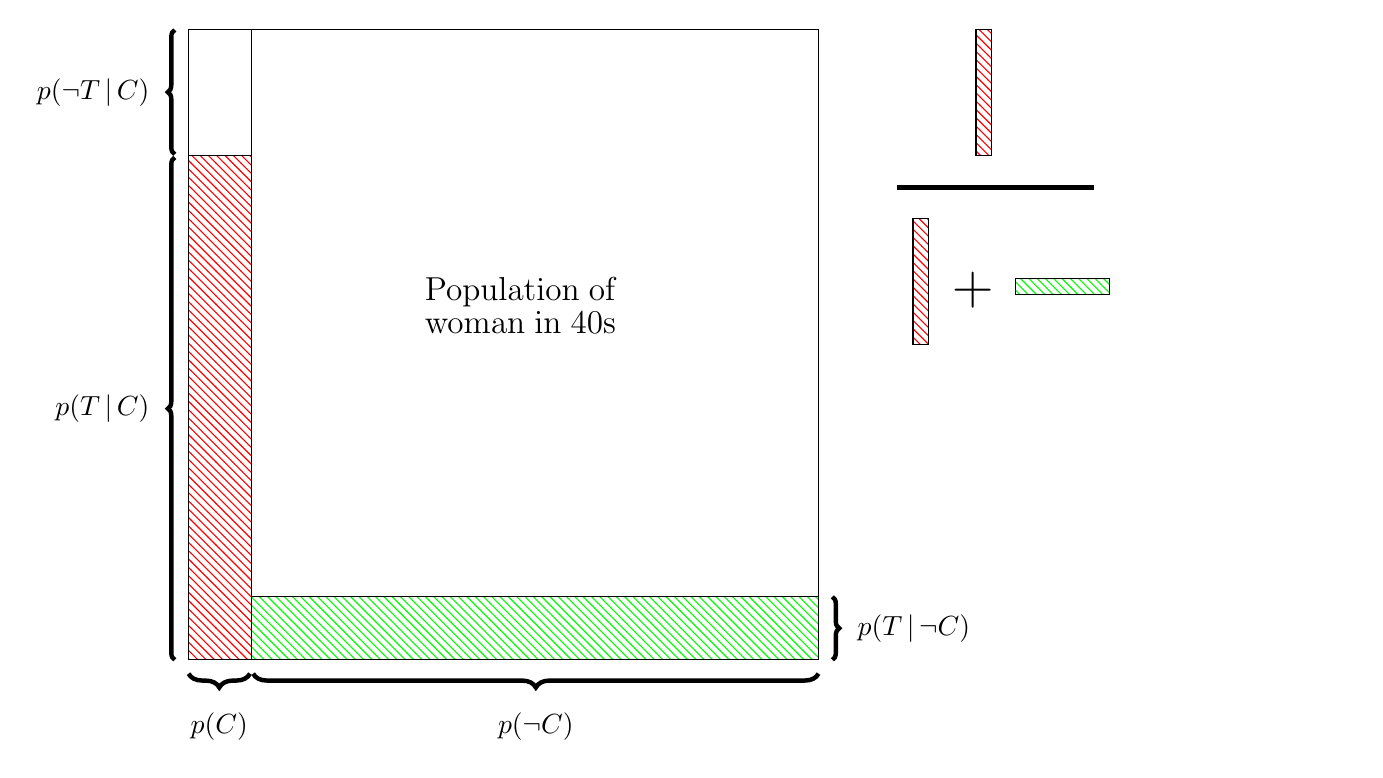
\begin{tikzpicture}

    \pgfmathsetmacro{\width}{8}
    \pgfmathsetmacro{\height}{8}
    \pgfmathsetmacro{\scl}{.25}
    
    \filldraw[black, fill=white] (0, 0) rectangle (\width, \height);
    \filldraw[black, fill=white] (0, 0) rectangle (.1*\width, \height);
    \draw[pattern=north west lines, pattern color=red] (0, 0) rectangle (.1*\width, .8*\height);
    \draw[pattern=north west lines, pattern color=green] (.1*\width, 0) rectangle (\width, .1*\height);

    \node[text width=3cm] at (.5*\width+.5, .5*\height+.5) {\large Population of woman in 40s};
    
    \draw[decorate, decoration = {brace, mirror, amplitude=5pt}, yshift=-5pt, ultra thick] (.1*\width+.02,0) --node[below=10pt]{$p(\neg C)$} (\width,0);

    \draw[decorate, decoration = {brace, mirror, amplitude=5pt}, yshift=-5pt, ultra thick] (0,0) --node[below=10pt]{$p(C)$} (.1*\width-0.02,0);

    \draw[decorate, decoration = {brace, mirror}, xshift=5pt, ultra thick] (\width,0) --node[right=5pt]{$p(T\,|\, \neg C)$} (\width,.1*\height);

    \draw[decorate, decoration = {brace}, xshift=-5pt, ultra thick] (0,0) --node[left=5pt]{$p(T\,|\, C)$} (0,.8*\height-0.02);
    \draw[decorate, decoration = {brace}, xshift=-5pt, ultra thick] (0,.8*\height+0.02) --node[left=5pt]{$p(\neg T\,|\, C)$} (0,\height);

    \draw[pattern=north west lines, pattern color=red] 
        (\width+2, .8*\height) 
        rectangle 
        (.1*\width*\scl + \width+2, .8*\height*\scl + .8*\height);
        
    \draw[black, -, ultra thick](\width+1, .75*\height) -- (\width+3.5, .75*\height);

    \draw[pattern=north west lines, pattern color=red] 
        (\width+1.2, .5*\height) 
        rectangle 
        (.1*\width*\scl + \width+1.2, .8*\height*\scl + .5*\height);

    \node[text width=5cm] at (\width+4.2, .5*\height+0.7) {\huge +};

    \draw[pattern=north west lines, pattern color=green] 
        (.1*\width + \width+1.7, .58*\height) 
        rectangle 
        (\width*\scl + \width+1.7, .1*\height*\scl + .58*\height);
    
\end{tikzpicture}
\caption{Bayes' rule visualisation where the probability $p(C \,|\, T)$ can be viewed as the proportion of a rectangle. In this case, the rectangle denotes the total population of woman including those that took the test and those who have cancer.}
\label{fig:bayes_vis}
\end{figure}

\newpage
\section{Bayesian Networks}

The \textbf{benefits of structure} are present in situations where feeding a mass of undigested data ought to result in good predictions about the data. Such naive approaches are limited by the fact that large quantities of \textit{variables} have even larger possible ways of interacting with one another, so that without some sensible \textit{assumptions}, we are unlikely to make a useful model. Furthermore, structure is important for computational \textit{tractability}. Given a distribution on $N$ binary variables $p(x_1,\dots,x_N)$, computing a marginal for $p(x_1)$ requires summing over the $2^{N-1}$ possible states of the other variables. 

To introduce structure, we can specify which variables are \textbf{independent} of other variables, which leads to a structured factorisation of the joint probability distribution. Consider
$$
    p(x_1, \dots, x_N) = \prod_{i = 1}^{N} \phi(x_i, x_{1:i})
$$
which becomes \textit{trivial} once we make \textbf{independence assumptions}. 

\textbf{Belief networks}, or \textbf{Bayesian networks}, are a convenient framework for representing independence assumptions. First, consider the following theorem regarding the type of graph in Bayesian networks.  
\\
\begin{theorem}
    \textbf{Directed Acyclic Graph (DAG).} A DAG is a graph $G$ with \textit{directed edges} (arrows on each link) between the nodes such that by following a path of nodes from one node to another along the direction of each edge, no path will \textit{revisit} a node. In a DAG, the ancestors of $B$ are those nodes which have a directed path ending in $B$. Conversely, the descendants of $A$ are those nodes which have a directed path starting at $A$.
\end{theorem}

\noindent Considering figure~\ref{fig:DAG_example}, the \textit{parents} of $x_4$ are $\text{pa}(x_4) = \{ x_1, x_2, x_3\}$. The \textit{children} of $x_4$ are $\text{ch}(x_4) = \{x_5, x_6\}$. The \textit{family} of a node is itself and its parents. The \textit{Markov blanket} of a node is its parents, children, and the parents of its children. In this case, the Markov blanket of $x_4$ is $\{ x_1, x_2, x_3, x_5, x_6, x_7\}$.

\begin{figure}[H]
    \begin{center}
        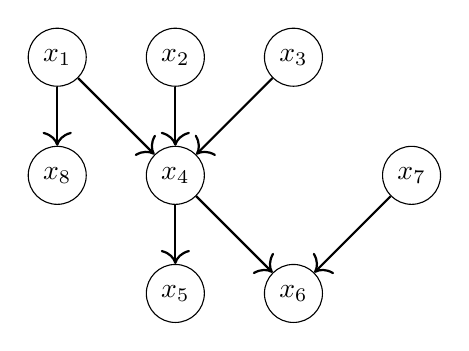
\begin{tikzpicture}
            \node[circle, draw] at (0, 4)   (x1) {$x_1$};
            \node[circle, draw] at (1.5, 4)   (x2) {$x_2$};
            \node[circle, draw] at (3, 4)   (x3) {$x_3$};
            \node[circle, draw] at (0, 2.5)   (x8) {$x_8$};
            \node[circle, draw] at (1.5, 2.5)   (x4) {$x_4$};
            \node[circle, draw] at (4.5, 2.5)   (x7) {$x_7$};
            \node[circle, draw] at (1.5, 1)   (x5) {$x_5$};
            \node[circle, draw] at (3, 1)   (x6) {$x_6$};

            \draw [-{To[scale=1.5]}, thick] (x1) -- (x8);
            \draw [-{To[scale=1.5]}, thick] (x1) -- (x4);
            \draw [-{To[scale=1.5]}, thick] (x2) -- (x4);
            \draw [-{To[scale=1.5]}, thick] (x3) -- (x4);
            \draw [-{To[scale=1.5]}, thick] (x4) -- (x5);
            \draw [-{To[scale=1.5]}, thick] (x4) -- (x6);
            \draw [-{To[scale=1.5]}, thick] (x7) -- (x6);
        \end{tikzpicture}
    \end{center}
    \caption{Example of a Directed Acyclic Graph (DAG).}
    \label{fig:DAG_example}
\end{figure}
% \leavevmode\newline 


% \\\\\\
\subsection{Motivation of Bayesian Networks}
To motivate the use-case of Bayesian networks, consider a joint probability of $4$ binary random variables ($A, B, C, D$), that have the states $\{0, 1\}$. To compute this probability, naively we would assume the need of specifying $2^4 = 16$ values. However, this is actually $2^4 - 1 = 15$, as the following shows. 
\begin{align*}
    p(A, B, C, D) &= p(A \,|\, B, C, D)p(B, C, D)\\
    &= p(A \,|\, B, C, D)p(B \,|\, C, D)p(C, D)\\
    &= p(A \,|\, B, C, D)p(B \,|\, C, D)p(C\,|\, D) p(D)
\end{align*}
Due to normalisation, we only need to know $p(A = 1\,|\, B, C, D)$, because $p(A = 0\,|\, B, C, D) = 1 - p(A = 1\,|\, B, C, D)$. This first term consists of $2^3 = 8$ states. The second conditional term, $p(B \,|\, C, D)$, consists of $2^2 = 4$ states, and $p(C\,|\,D) = 2$ states, $p(D) = 1$ state. Thus, $8+4+2+1 = 15 = 2^4 - 1$. As the amount of random variables grows, the amount of states grows exponentially. This is impractical, and thus, promotes simplification.

\subsubsection{Conditional independence assumption}
To simplify the computationally demanding joint probability problem, we can make assumptions about the relationship of the variables. 

As an example, consider the following. One morning Adam's car does not start. He wants to know whether the car was sabotaged by stone martens or if there is a defect in the car. His neighbour, Bob, also cannot drive to work this morning because of his broken car. We can model this situation as:
\begin{table}[H]
    \centering
    \begin{tabular}{ll}
        $A \in \{0, 1\}$ & $A = 1$ means that Adam's car is broken, and 0 otherwise. \\
        $B \in \{0, 1\}$ & $B = 1$ means that Bob's car is broken, and 0 otherwise. \\
        $C \in \{0, 1\}$ & $C = 1$ means that Adam's car was sabotaged by stone martens, and 0 otherwise. \\
        $D \in \{0, 1\}$ & $D = 1$ means that the car has a naturally occurring defect, and 0 otherwise. 
    \end{tabular}    
\end{table}

\noindent We can make assumptions based on \textbf{constraints} in the system. We can assume that Adam's car being broken is only directly dependent on variables $C$ and $D$. So, instead of computing the conditional probability the usual way, we can make a \textit{conditional independence assumption}
$$
    p(A\,|\, B, C, D) = p(A\,|\, C, D)
$$
Likewise, $p(B \,|\, A, C, D) = p(B \,|\, D)$, and $p(C \,|\, A, B, D) = p(C)$, and $p(D \,|\, A, B, C) = p(D)$. The following graph describes these relationships as a Bayesian network.

\begin{figure}[H]
    \centering
    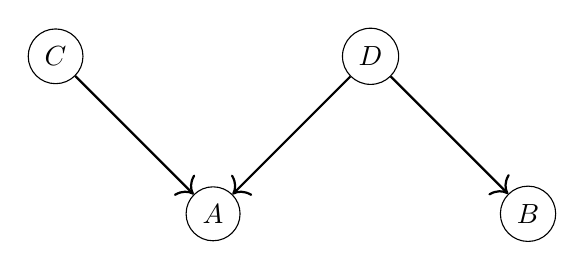
\begin{tikzpicture}
        \node[circle, draw] at (0, 2)   (C) {$C$};
        \node[circle, draw] at (2, 0)   (A) {$A$};
        \node[circle, draw] at (4, 2)   (D) {$D$};
        \node[circle, draw] at (6, 0)   (B) {$B$};

        \draw [-{To[scale=1.5]}, thick] (C) -- (A);
        \draw [-{To[scale=1.5]}, thick] (D) -- (A);
        \draw [-{To[scale=1.5]}, thick] (D) -- (B);
    \end{tikzpicture}
    \caption{Example Bayesian network}
    \label{fig:my_label}
\end{figure}

\noindent Compared to the naive approach of specifying the amount of values of a joint probability distribution, which is $2^4 - 1 = 15$ values for the states, now, the amount is reduced to only 8 values. We can now specify the probabilities of these variables. 

\subsubsection{Inference}

\noindent Let the prior probabilities of $C$ and $D$ be 
\begin{itemize}
    \item $p(C=1) = 0.05$
    \item $p(D=1) = 0.1$ .  
\end{itemize}
The remaining probabilities are
\begin{itemize}
    \item $p(B=1 \,|\, D=1) = 1$.
    \item $p(B=1 \,|\, D=0) = 0.4$, for when the car was possibly broken by someone.
    \item $p(A=1 \,|\, C=1, D=0) = 0.95$, because sometimes the stone martens are unsuccessful.
    \item $p(A=1 \,|\, C=1, D=1) = 1$,  
    \item $p(A=1 \,|\, C=0, D=1) = 1$.
    \item $p(A=1 \,|\, C=0, D=0) = 0.2$, for when there was another unknown cause for Adam's car being broken.
\end{itemize}  

\noindent To infer what the probability is that stone martens sabotaged Adam's car, given that Adam's car is broken, $p(C=1 \,|\, A=1)$, we can do the following. 

\begin{align*}
    &p(C=1 \,|\, A=1) = \frac{p(C=1, A=1)}{p(A=1)} = \frac{\sum_{B, D} p(A=1, B, C=1, D)}{\sum_{B, C, D} p(A=1, B, C, D)} \\[1em]
    &= \frac{\sum_{B, D} p(A=1 \,|\, C=1, D)p(B \,|\, D)p(D)p(C=1)}{\sum_{B, C, D} p(A=1 \,|\, C, D) p(B \,|\, D) p(C) p(D)} \\[1em]
    &= \frac{p(C=1) \sum_{B, D} p(A=1 \,|\, C=1, D)p(B \,|\, D)p(D)}{\sum_{B, C, D} p(A=1 \,|\, C, D) p(B \,|\, D) p(C) p(D)} \\[1em]
    &= \dfrac{0.05 \cdot (0.95 \cdot 0.6 \cdot 0.9 + 1 \cdot 0 \cdot 0.1 + 0.95 \cdot 0.4 \cdot 0.9 + 1 \cdot 1 \cdot 0.1)}{\splitdfrac{0.2 \cdot 0 \cdot 0.95 \cdot 0.9 + 1 \cdot 0 \cdot 0.95 \cdot 0.1 + 0.2 \cdot 0.4 \cdot 0.95 \cdot 0.9 + 1 \cdot 1 \cdot 0.95 \cdot 0.1 }{ + 0.95 \cdot 0 \cdot 0.05 \cdot 0.9 + 1 \cdot 0 \cdot 0.05 \cdot 0.1 + 0.95 \cdot 0.4 \cdot 0.05 \cdot 0.9 + 1 \cdot 1 \cdot 0.05 \cdot 0.1}} \\[1em]
    &= \frac{0.05 \cdot (0.95 \cdot 0.6 \cdot 0.9 + 0.95 \cdot 0.4 \cdot 0.9 + 1 \cdot 1 \cdot 0.1)}{0.2 \cdot 0.4 \cdot 0.95 \cdot 0.9 + 1 \cdot 1 \cdot 0.95 \cdot 0.1 + 0.95 \cdot 0.4 \cdot 0.05 \cdot 0.9 + 1 \cdot 1 \cdot 0.05 \cdot 0.1} \\[1em]
    &= \frac{0.05 \cdot 0.955}{0.1855} = 0.2574
\end{align*}

\noindent The above result tells us that the \textbf{posterior belief} that Adam's car was sabotaged increases above the \textbf{prior belief}, which was $0.05$, due to the \textbf{evidence} that Adam's car is broken.

\textbf{Remark}: due to the commutativity of the joint probability, i.e., $p(A, B) = p(B, A)$, it is also arbitrary to chose how to define the order of the conditional joint probability. We could define $p(X, Y, Z)$ equally valid as
\begin{align*}
    &p(Z \,|\, X, Y) p(Y \,|\, X) p(X) \\
    &p(X \,|\, Y, Z) p(Y \,|\, Z) p(Z) \\
    &p(X \,|\, Y, Z) p(Z \,|\, Y) p(Y) \\
    &p(Y \,|\, X, Z) p(Z \,|\, X) p(X) \\
    &p(Y \,|\, X, Z) p(X \,|\, Z) p(Z) \\
    &p(Z \,|\, X, Y) p(X \,|\, Y) p(Y)
\end{align*}
Usually, the variables that have no conditional dependence are the \textbf{root causes} of the Bayesian network.

\subsection{Definition of Bayesian Networks}
\begin{theorem}
    \textbf{Bayesian Network.} A Bayesian network or belief network is a distribution of the form
    $$
        p(x_1, \dots, x_N) = \prod_{i=1}^N p(x_i \,|\, \text{pa}(x_i))
    $$
    where pa($x_i$) represents the \textit{parental} variables of variable $x_i$. A BN corresponds to a Directed Acyclic Graph~(DAG), with the $i$th node in the graph corresponding to the factor $p(x_i\,|\,\text{pa}(x_i))$.
\end{theorem}


\subsubsection{Colliders}
\begin{theorem}
    \textbf{Collider.} Given a path $\mathcal{P}$, a collider is a node $C$ on $\mathcal{P}$ with neighbours $A$ and $B$ on $\mathcal{P}$, such that $A \rightarrow C \leftarrow B$.
    \begin{center}
        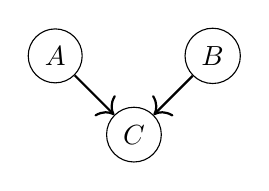
\begin{tikzpicture}
            \node[circle, draw] at (0, 1)   (a) {$A$};
            \node[circle, draw] at (1, 0)   (c) {$C$};
            \node[circle, draw] at (2, 1)   (b) {$B$};
            
            \draw [-{To[scale=1.5]}, thick] (a) -- (c);
            \draw [-{To[scale=1.5]}, thick] (b) -- (c);
        \end{tikzpicture}
    \end{center}
\end{theorem}

\noindent As an example of a collider, consider the following. Let $Z$ represent whether or not a baseball field is wet, $X$ represent if it is raining, and $Y$ represent if the sprinkler system is on. The BN is of the form: $X \rightarrow Z \leftarrow Y$. If we are told that the sprinkler system is on ($Y=1$), it does not change our belief regarding whether or not it is raining ($X \in \{1, 0\}$). 

However, if we are told that the baseball field is wet ($Z=1$), and then told that it is not raining ($X=0$), then we will \textbf{increase} our belief that the sprinkler system is on. 

Therefore, as long as we do not know the value of $Z$, then $X$ and $Y$ will be \textit{d-separated}. However, if we have information about $Z$, then the path is no longer blocked, and thus $X$ and $Y$ may influence each other. 
\\
\\
\noindent More formally, given the network $A \rightarrow C \leftarrow B$, we define the full joint probability as 
$$
    p(A, B, C) = p(C \,|\, A, B) p(A) p(B)
$$
in which $A$ and $B$ are both \textit{causes} that determine the \textit{effect} $C$.

\begin{center}
    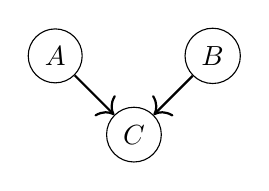
\begin{tikzpicture}
        \node[circle, draw] at (0, 1)   (a) {$A$};
        \node[circle, draw] at (1, 0)   (c) {$C$};
        \node[circle, draw] at (2, 1)   (b) {$B$};
        
        \draw [-{To[scale=1.5]}, thick] (a) -- (c);
        \draw [-{To[scale=1.5]}, thick] (b) -- (c);
    \end{tikzpicture}
\end{center}

\noindent \textbf{Marginalising} over $C$ makes $A$ and $B$ independent. $A$ and $B$ are unconditionally independent, $p(A, B) = p(A)p(B)$. In the absence of any information about the effect $C$, we retain this belief. This result shows due to normalisation of $\sum_C p(C \,|\, A, B) = 1$, which disappears in the equation leaving only $p(A)p(B)$. See figure~\ref{fig:margC}.
\begin{align*}
    p(A, B) &= \sum_C p(A, B, C)\\ 
    &= \sum_C p(C \,|\, A, B)p(A)p(B)\\ 
    &= p(A)p(B) \sum_C p(C \,|\, A, B)\\ 
    &= p(A)p(B) \cdot 1 = p(A)p(B)
\end{align*}
\begin{figure}[H]
    \centering
    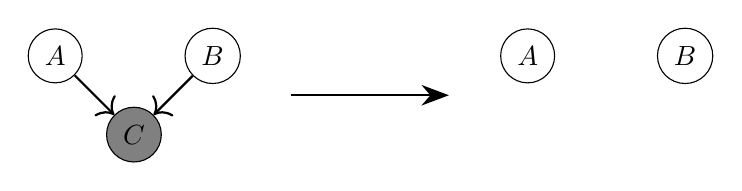
\begin{tikzpicture}
        \node[circle, draw] at (0, 1)   (a) {$A$};
        \node[circle, draw, fill=gray] at (1, 0)   (c) {$C$};
        \node[circle, draw] at (2, 1)   (b) {$B$};
        \draw [-{To[scale=1.5]}, thick] (a) -- (c);
        \draw [-{To[scale=1.5]}, thick] (b) -- (c);

        \node[circle, draw] at (6, 1)   (a_n) {$A$};
        \node[circle, draw] at (8, 1)   (b_n) {$B$};
        % \draw [thick] (a_n) -- (b_n);

        \draw [-{Stealth[scale=1.5]}, thick] (3, .5) -- (5, .5);
    \end{tikzpicture}
    \caption{Marginalising over $C$ leads to unconditional independence between $A$ and $B$.}
    \label{fig:margC}
\end{figure}

\noindent \textbf{Conditioning} on $C$ makes $A$ and $B$ (graphically) dependent. In general, $p(A, B \,|\, C) \neq p(A\,|\,C)p(B\,|\,C)$. Knowing the effect of $C$ changes the belief of the causes $A$ and $B$, as depicted in figure~\ref{fig:condC}.

\begin{figure}[H]
    \centering
    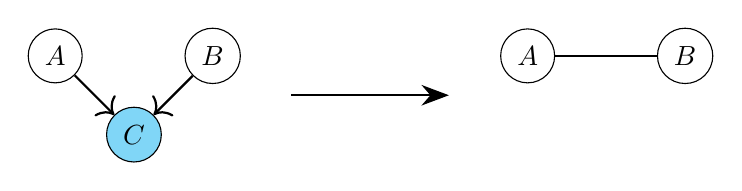
\begin{tikzpicture}
        \node[circle, draw] at (0, 1)   (a) {$A$};
        \node[circle, draw, fill=cyan!50] at (1, 0)   (c) {$C$};
        \node[circle, draw] at (2, 1)   (b) {$B$};
        \draw [-{To[scale=1.5]}, thick] (a) -- (c);
        \draw [-{To[scale=1.5]}, thick] (b) -- (c);

        \node[circle, draw] at (6, 1)   (a_n) {$A$};
        \node[circle, draw] at (8, 1)   (b_n) {$B$};
        \draw [thick] (a_n) -- (b_n);

        \draw [-{Stealth[scale=1.5]}, thick] (3, .5) -- (5, .5);
    \end{tikzpicture}
    \caption{Conditioning on $C$ leads to dependence between $A$ and $B$.}
    \label{fig:condC}
\end{figure}

\noindent This same result holds when the directed path is extended beyond the collider $C$ by another node $D$. Again, $p(A, B \,|\, D) \neq p(A\,|\,D)p(B\,|\,D)$, as can be seen in figure~\ref{fig:condD}.

\begin{figure}[H]
    \centering
    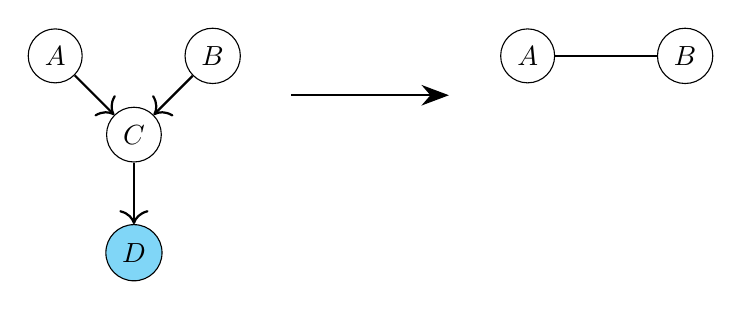
\begin{tikzpicture}
        \node[circle, draw] at (0, 1)   (a) {$A$};
        \node[circle, draw] at (1, 0)   (c) {$C$};
        \node[circle, draw] at (2, 1)   (b) {$B$};
        \node[circle, draw, fill=cyan!50] at (1, -1.5)   (d) {$D$};
        \draw [-{To[scale=1.5]}, thick] (a) -- (c);
        \draw [-{To[scale=1.5]}, thick] (b) -- (c);
        \draw [-{To[scale=1.5]}, thick] (c) -- (d);

        \node[circle, draw] at (6, 1)   (a_n) {$A$};
        \node[circle, draw] at (8, 1)   (b_n) {$B$};
        \draw [thick] (a_n) -- (b_n);

        \draw [-{Stealth[scale=1.5]}, thick] (3, .5) -- (5, .5);
    \end{tikzpicture}
    \caption{Conditioning on $D$ leads to dependence between $A$ and $B$.}
    \label{fig:condD}
\end{figure}

\subsection{d-connection and d-separation}

\subsubsection{Intuition}

\textit{d-separation} is a criterion for deciding, from a given DAG, whether a set of variables $X$ is independent of another set $Y$, given a third set $Z$. The idea is to associate \textbf{dependence} with \textbf{connectedness} (i.e., the existence of a connecting path) and \textbf{independence} with \textbf{unconnected-ness} or \textbf{separation}. We can define \textbf{active} and \textbf{inactive} paths between nodes in the Bayesian network. A path is active if every node on the path is active. A node is active if it carries \textbf{information} (\textbf{dependence}).  
\begin{itemize}
    \item[] Nodes $x$ and $y$ are \textbf{d-connected} if there is any \textit{active} path between them.
    \item[] Nodes $x$ and $y$ are \textbf{d-separated} if there is no path between them that is \textit{active}.
\end{itemize}
\noindent First, we consider the possible variants of active and inactive paths provided that the conditioning set $Z$ is empty. 
\begin{align}
    & A \rightarrow C \rightarrow B \\
    & A \leftarrow C \leftarrow B \\
    & A \leftarrow C \rightarrow B \\
    & A \rightarrow C \leftarrow B
\end{align}

\noindent In the first case, (1), the path is directed from $A$ to $B$ through $C$, in the second case~(2), the path is directed from $B$ to $A$ through $C$, and the third (3), there is a pair of directed paths from $C$ to $A$, and from $C$ to $B$. In terms of \textbf{causality}, (1) $A$ is an indirect cause of $B$, (2) $B$ is an indirect cause of $A$, and in the third case~(3), $C$ is the \textit{common cause} of both $A$ and $B$. Relative to an empty conditioning set $Z$, all three cases (1), (2), (3), are \textit{active}. 

Notice that the fourth case is a collider, and is the only one that is \textit{inactive}. Intuitively, this can be explained by $A$ and $B$ having a \textit{common effect} in $C$, but no causal relation between them. 
\\
\\
\noindent If we consider the same paths (1), (2), (3), (4), above, but now with a non-empty conditioning set $Z = \{C\}$, then the status with respect to active or inactive nodes flip-flops i.e., active becomes inactive, and vice versa. 

In the first and second case, (1), (2), $C$ now blocks the path between $A$ and $B$, i.e., the information (dependence) cannot flow between them because the conditional $C$ is known. Likewise in the third case, (3), due to a known $C$ that causes $A$ and $B$ to not be dependent on each other's values. The fourth case, (4), now is active due to the common effect $C$ being known, which associates the values of $A$ and $B$. If $C$ is known, and thereafter, $A$ is known, that changes the belief of $B$. 

Consider an example in which there are two independent \textit{causes} of a car refusing to start $C = \{0, 1\}$. Having no gas $G = \{0, 1\}$ and having a dead battery $B = \{0, 1\}$.
$$
    B \rightarrow C \leftarrow G
$$
Knowing that the battery is charged ($B = 0$) provides no additional information about whether there is gas, but knowing that the battery is charged ($B = 0$) \textit{after} finding out that the car will not start ($C = 1$) leads to an increase in the belief that the gas tank must be empty ($G = 1$). So \textit{independent causes} are made \textit{dependent} by conditioning on a \textit{common effect}, which in the directed graph representing the causal structure is the same as \textbf{conditioning on a collider}. 

Furthermore, not only does conditioning on a collider activate the path but the path is also activated when conditioning on the \textbf{descendants} of a collider.  

\subsubsection{Formal definition}

\begin{theorem}
    \textbf{d-connected and d-separated}. If $G$ is a directed graph in which $X$, $Y$ and $Z$ are disjoint sets of nodes, then $X$ and $Y$ are \textit{d-connected} by $Z$ in $G$ if and only if there exists an \textbf{undirected path} $U$ between some node in $X$ and some node in $Y$ such that for every collider $C$ on $U$, either $C$ or a descendent of $C$ is in $Z$, and no non-collider on $U$ is in $Z$.
    \\\\
    $X$ and $Y$ are \textit{d-separated} by $Z$ in $G$ if and only if they are not d-connected by $Z$ in $G$.
\end{theorem}

\subsubsection{Examples of determining conditional independence}

\noindent As an example, consider the DAG in figure~\ref{fig:ex_DAG}, in which we want to know whether nodes $A$ and $B$ are unconditionally independent, i.e., $A \indep B \,|\, \emptyset$. 

\begin{figure}[H]
    \centering
    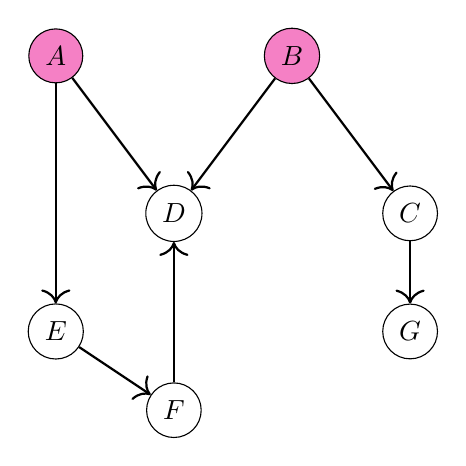
\begin{tikzpicture}
        \node[circle, draw, fill=magenta!50] at (0, 4)   (A) {$A$};
        \node[circle, draw, fill=magenta!50] at (3, 4)   (B) {$B$};
        \node[circle, draw] at (4.5, 2)   (C) {$C$};
        \node[circle, draw] at (1.5, 2)   (D) {$D$};
        \node[circle, draw] at (0, .5)   (E) {$E$};
        \node[circle, draw] at (1.5, -.5)   (F) {$F$};
        \node[circle, draw] at (4.5, .5)   (G) {$G$};
        \draw [-{To[scale=1.5]}, thick] (A) -- (D);
        \draw [-{To[scale=1.5]}, thick] (B) -- (D);
        \draw [-{To[scale=1.5]}, thick] (A) -- (E);
        \draw [-{To[scale=1.5]}, thick] (E) -- (F);
        \draw [-{To[scale=1.5]}, thick] (F) -- (D);
        \draw [-{To[scale=1.5]}, thick] (B) -- (C);
        \draw [-{To[scale=1.5]}, thick] (C) -- (G);
    \end{tikzpicture}
    \caption{Example Bayesian network on which we are interested in determining the independence between $A$ and $B$.}
    \label{fig:ex_DAG}
\end{figure}

\noindent To determine whether the conditioning statement, $A \indep B \,|\, \emptyset$, is true, we need to determine if the paths from $A$ to $B$ are active or inactive. There are 2 paths: 
\begin{align}
    A - D - B \\
    A - E - F - D - B
\end{align}

\begin{center}
    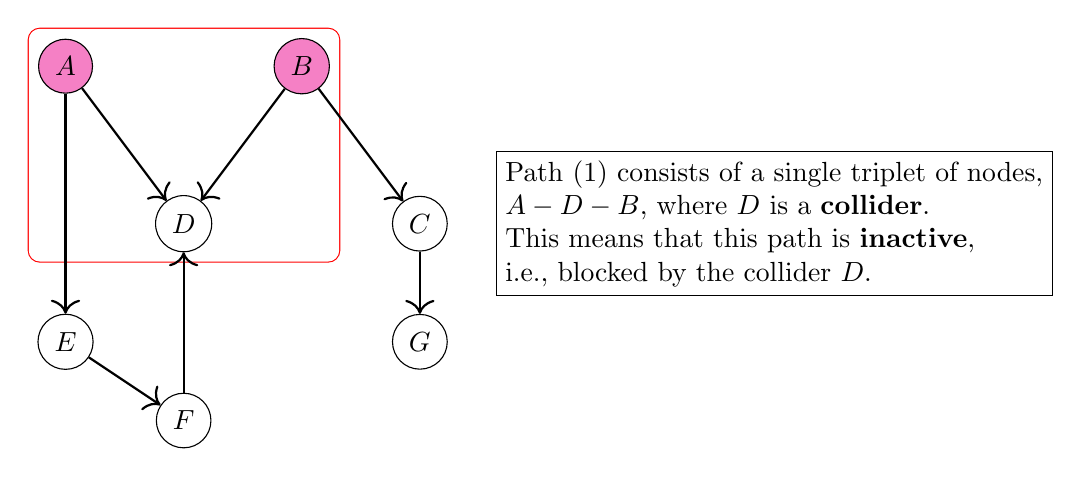
\begin{tikzpicture}
        \node[circle, draw, fill=magenta!50] at (0, 4)   (A) {$A$};
        \node[circle, draw, fill=magenta!50] at (3, 4)   (B) {$B$};
        \node[circle, draw] at (4.5, 2)   (C) {$C$};
        \node[circle, draw] at (1.5, 2)   (D) {$D$};
        \node[circle, draw] at (0, .5)   (E) {$E$};
        \node[circle, draw] at (1.5, -.5)   (F) {$F$};
        \node[circle, draw] at (4.5, .5)   (G) {$G$};
        \draw [-{To[scale=1.5]}, thick] (A) -- (D);
        \draw [-{To[scale=1.5]}, thick] (B) -- (D);
        \draw [-{To[scale=1.5]}, thick] (A) -- (E);
        \draw [-{To[scale=1.5]}, thick] (E) -- (F);
        \draw [-{To[scale=1.5]}, thick] (F) -- (D);
        \draw [-{To[scale=1.5]}, thick] (B) -- (C);
        \draw [-{To[scale=1.5]}, thick] (C) -- (G);

        \node[draw,align=left] at (9,2) {Path (1) consists of a single triplet of nodes, \\$A - D - B$, where $D$ is a \textbf{collider}.\\ This means that this path is \textbf{inactive}, \\i.e., blocked by the collider $D$.};
        
        \pgfdeclarelayer{bg}
        \pgfsetlayers{bg,main}
        \begin{pgfonlayer}{bg}
             \node (box) [draw=red,line width=.8pt,rounded corners,fit = (A) (B) (D)] {};
             
             \node (box) [fill=white,rounded corners,fit = (A) (B) (D)] {};
        \end{pgfonlayer}
    \end{tikzpicture}
\end{center}

\noindent Recall that two nodes are \textbf{d-connected} if there is any active path between them. Therefore, we need to determine whether path (2) is active or inactive.  

\begin{center}
    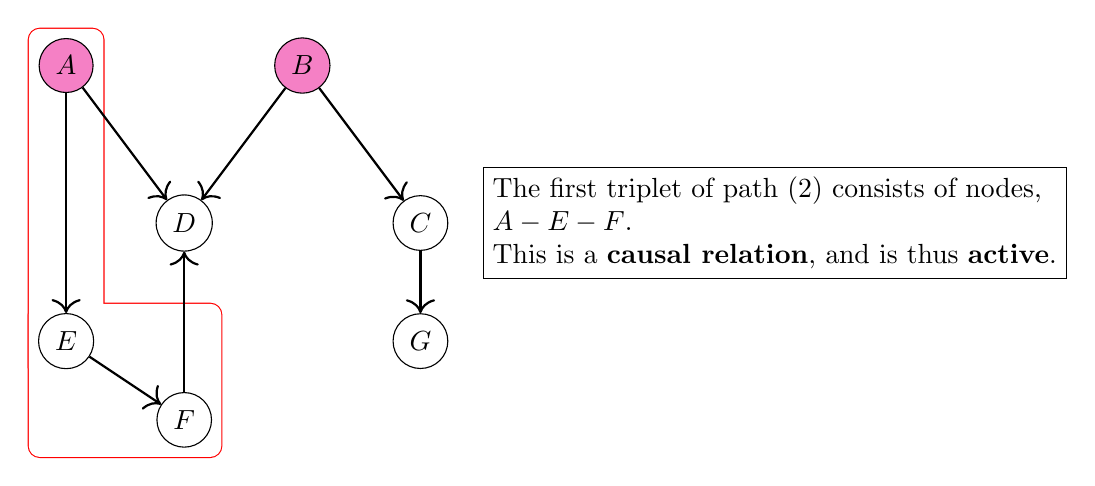
\begin{tikzpicture}
        \node[circle, draw, fill=magenta!50] at (0, 4)   (A) {$A$};
        \node[circle, draw, fill=magenta!50] at (3, 4)   (B) {$B$};
        \node[circle, draw] at (4.5, 2)   (C) {$C$};
        \node[circle, draw] at (1.5, 2)   (D) {$D$};
        \node[circle, draw] at (0, .5)   (E) {$E$};
        \node[circle, draw] at (1.5, -.5)   (F) {$F$};
        \node[circle, draw] at (4.5, .5)   (G) {$G$};
        \draw [-{To[scale=1.5]}, thick] (A) -- (D);
        \draw [-{To[scale=1.5]}, thick] (B) -- (D);
        \draw [-{To[scale=1.5]}, thick] (A) -- (E);
        \draw [-{To[scale=1.5]}, thick] (E) -- (F);
        \draw [-{To[scale=1.5]}, thick] (F) -- (D);
        \draw [-{To[scale=1.5]}, thick] (B) -- (C);
        \draw [-{To[scale=1.5]}, thick] (C) -- (G);

        \node[draw,align=left] at (9,2) {The first triplet of path (2) consists of nodes, \\$A - E - F$.\\ This is a \textbf{causal relation}, and is thus \textbf{active}.};
        
        \pgfdeclarelayer{bg}
        \pgfsetlayers{bg,main}
        \begin{pgfonlayer}{bg}
             \node (box) [draw=red,line width=.8pt,rounded corners,fit = (A) (E)] {};
             \node (box) [draw=red,line width=.8pt,rounded corners,fit = (E) (F)] {};
             
             \node (box) [fill=white,rounded corners,fit = (A) (E)] {};
            \node (box) [fill=white,rounded corners,fit = (E) (F)] {};
        \end{pgfonlayer}
    \end{tikzpicture}
\end{center}

\begin{center}
    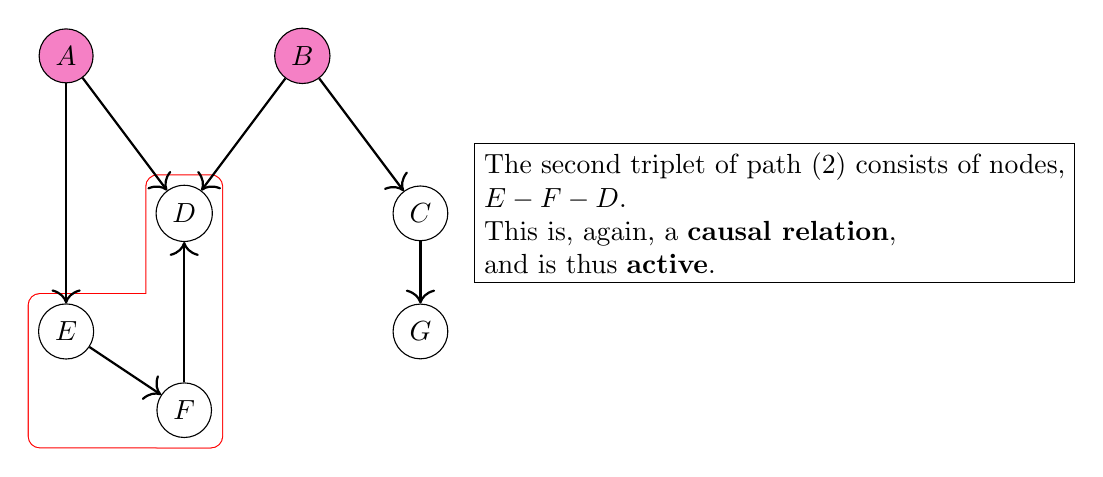
\begin{tikzpicture}
        \node[circle, draw, fill=magenta!50] at (0, 4)   (A) {$A$};
        \node[circle, draw, fill=magenta!50] at (3, 4)   (B) {$B$};
        \node[circle, draw] at (4.5, 2)   (C) {$C$};
        \node[circle, draw] at (1.5, 2)   (D) {$D$};
        \node[circle, draw] at (0, .5)   (E) {$E$};
        \node[circle, draw] at (1.5, -.5)   (F) {$F$};
        \node[circle, draw] at (4.5, .5)   (G) {$G$};
        \draw [-{To[scale=1.5]}, thick] (A) -- (D);
        \draw [-{To[scale=1.5]}, thick] (B) -- (D);
        \draw [-{To[scale=1.5]}, thick] (A) -- (E);
        \draw [-{To[scale=1.5]}, thick] (E) -- (F);
        \draw [-{To[scale=1.5]}, thick] (F) -- (D);
        \draw [-{To[scale=1.5]}, thick] (B) -- (C);
        \draw [-{To[scale=1.5]}, thick] (C) -- (G);

        \node[draw,align=left] at (9,2) {The second triplet of path (2) consists of nodes, \\$E - F - D$.\\ This is, again, a \textbf{causal relation}, \\ and is thus \textbf{active}.};
        
        \pgfdeclarelayer{bg}
        \pgfsetlayers{bg,main}
        \begin{pgfonlayer}{bg}
             \node (box) [draw=red,line width=.8pt,rounded corners,fit = (E) (F)] {};
             \node (box) [draw=red,line width=.8pt,rounded corners,fit = (F) (D)] {};
             
             \node (box) [fill=white,rounded corners,fit = (E) (F)] {};
            \node (box) [fill=white,rounded corners,fit = (F) (D)] {};
        \end{pgfonlayer}
    \end{tikzpicture}
\end{center}

\begin{center}
    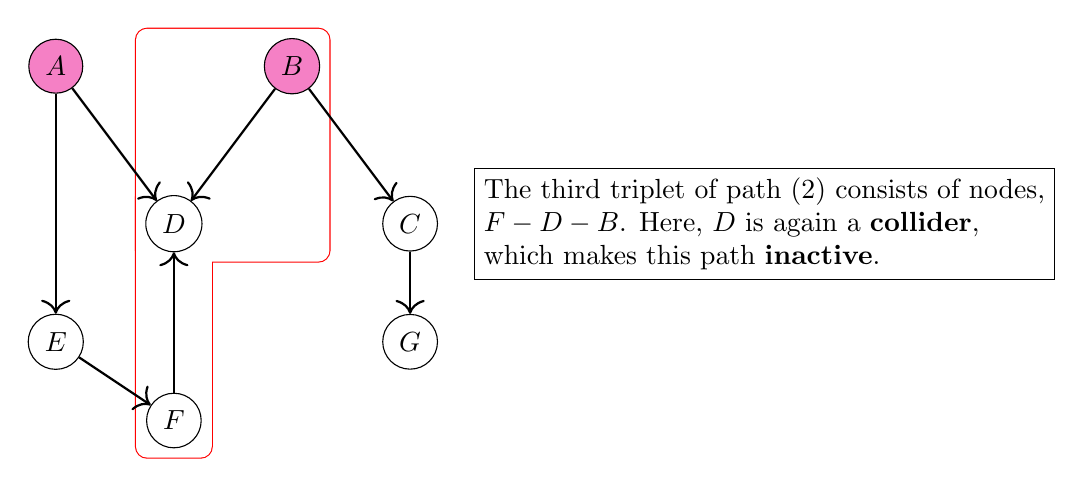
\begin{tikzpicture}
        \node[circle, draw, fill=magenta!50] at (0, 4)   (A) {$A$};
        \node[circle, draw, fill=magenta!50] at (3, 4)   (B) {$B$};
        \node[circle, draw] at (4.5, 2)   (C) {$C$};
        \node[circle, draw] at (1.5, 2)   (D) {$D$};
        \node[circle, draw] at (0, .5)   (E) {$E$};
        \node[circle, draw] at (1.5, -.5)   (F) {$F$};
        \node[circle, draw] at (4.5, .5)   (G) {$G$};
        \draw [-{To[scale=1.5]}, thick] (A) -- (D);
        \draw [-{To[scale=1.5]}, thick] (B) -- (D);
        \draw [-{To[scale=1.5]}, thick] (A) -- (E);
        \draw [-{To[scale=1.5]}, thick] (E) -- (F);
        \draw [-{To[scale=1.5]}, thick] (F) -- (D);
        \draw [-{To[scale=1.5]}, thick] (B) -- (C);
        \draw [-{To[scale=1.5]}, thick] (C) -- (G);

        \node[draw,align=left] at (9,2) {The third triplet of path (2) consists of nodes, \\$F - D - B$. Here, $D$ is again a \textbf{collider}, \\ which makes this path \textbf{inactive}.};
        
        \pgfdeclarelayer{bg}
        \pgfsetlayers{bg,main}
        \begin{pgfonlayer}{bg}
             \node (box) [draw=red,line width=.8pt,rounded corners,fit = (F) (D)] {};
             \node (box) [draw=red,line width=.8pt,rounded corners,fit = (D) (B)] {};
             
             \node (box) [fill=white,rounded corners,fit = (F) (D)] {};
            \node (box) [fill=white,rounded corners,fit = (D) (B)] {};
        \end{pgfonlayer}
    \end{tikzpicture}
\end{center}

\noindent We have concluded that both paths, (1), (2), are \textbf{inactive}, and thus blocked by the collider $D$. In other words, $A$ and $B$ are \textbf{d-separated}. This means that $A \indep B \,|\, \emptyset = true$, i.e., $A$ and $B$ are (graphically) unconditionally independent. 
\\\\
Suppose the conditioning statement was $A \indep B \,|\, D$, then the result would be different.

\begin{center}
    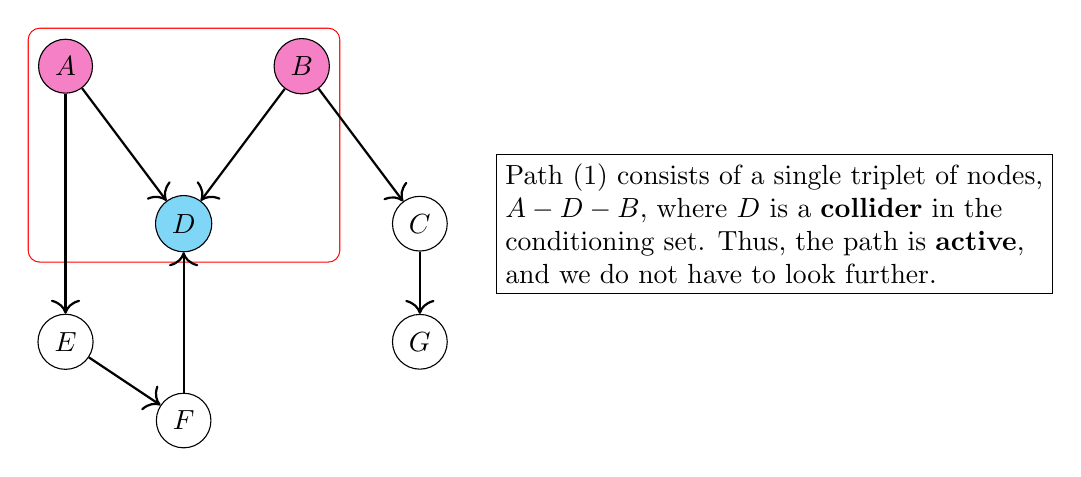
\begin{tikzpicture}
        \node[circle, draw, fill=magenta!50] at (0, 4)   (A) {$A$};
        \node[circle, draw, fill=magenta!50] at (3, 4)   (B) {$B$};
        \node[circle, draw] at (4.5, 2)   (C) {$C$};
        \node[circle, draw, fill=cyan!50] at (1.5, 2)   (D) {$D$};
        \node[circle, draw] at (0, .5)   (E) {$E$};
        \node[circle, draw] at (1.5, -.5)   (F) {$F$};
        \node[circle, draw] at (4.5, .5)   (G) {$G$};
        \draw [-{To[scale=1.5]}, thick] (A) -- (D);
        \draw [-{To[scale=1.5]}, thick] (B) -- (D);
        \draw [-{To[scale=1.5]}, thick] (A) -- (E);
        \draw [-{To[scale=1.5]}, thick] (E) -- (F);
        \draw [-{To[scale=1.5]}, thick] (F) -- (D);
        \draw [-{To[scale=1.5]}, thick] (B) -- (C);
        \draw [-{To[scale=1.5]}, thick] (C) -- (G);

        \node[draw,align=left] at (9,2) {Path (1) consists of a single triplet of nodes, \\$A - D - B$, where $D$ is a \textbf{collider} in the \\conditioning set. Thus, the path is \textbf{active},\\ and we do not have to look further.};
        
        \pgfdeclarelayer{bg}
        \pgfsetlayers{bg,main}
        \begin{pgfonlayer}{bg}
             \node (box) [draw=red,line width=.8pt,rounded corners,fit = (A) (B) (D)] {};
             
             \node (box) [fill=white,rounded corners,fit = (A) (B) (D)] {};
        \end{pgfonlayer}
    \end{tikzpicture}
\end{center}

\noindent In this case, we condition on $D$ by which the first path $A-D-B$ is \textbf{active} resulting in the conclusion that $A \indep B \,|\, D = false$. In other words, $A$ and $B$ are \textbf{d-connected}. 

\subsection{Markov Blanket}

The \textbf{Markov blanket} of a variable $X$ carries all information about $X$. That is, 
$$
    MB(X) = \text{pa}(X) \cup \text{ch}(X) \cup \bigcup \{\text{pa}(Y) \giv y \in \text{ch}(X), X \neq Y\}.
$$
\noindent Then, for any other variable $Z$ that is not in the Markov blanket of $X$, i.e., $Z \in \mathcal{X} \text{\textbackslash} \{X \cup MB(X)\}$, implies that $X \indep Z \giv MB(X)$. Consider figure~\ref{fig:ex_DAG}, in which the Markov blanket of $E$ is $MB(E) = \{A, F\}$. Thus, conditioning on the Markov blanket, will make $E$ independent of all other variables not in its Markov blanket.

\subsection{Markov Equivalence}

\begin{theorem}
    \textbf{Markov Equivalence.} Two graphs are Markov equivalent if they both represent the same set of conditional independence statements. This definition holds for both directed and undirected graphs. 
\end{theorem}

\noindent Suppose we construct a Bayesian network of the form $A \rightarrow C \leftarrow B$, from which the set of conditional independence statements consists of a single element, $A \indep B \,|\, \emptyset$. 

Now consider the Bayesian network $A \rightarrow C \leftarrow B \leftarrow A$. Are the first and second networks Markov equivalent? The answer is no, because the set of conditional independence statements for this second network is empty, as $A \indep B \,|\, \emptyset = false$.

\subsubsection{Determining Markov equivalence}

The procedure to determine Markov equivalence between two graphs is as follows. Start by identifying the so-called \textbf{immortalities}. An immortality is a configuration of 3 nodes, $A, B, C$, such that $C$ is a child of $A$ and $B$, i.e., a collider structure, with $A$ and $B$ not directly connected. Next, define the \textbf{skeleton} of the graph by removing the direction of the arrows. 

Finally, two DAGs represent the same set of independence assumptions, i.e., Markov equivalence, if and only if they have the same skeleton and the same set of immortalities. 

\subsubsection{Example: determining Markov equivalence}

Consider the DAG in figure~\ref{fig:mk}a, how many Markov equivalent graphs can be constructed from this graph? To answer this question, we first need to identify the immortalities. The triplet $A \rightarrow C \leftarrow B$ is an immortality, as well as the triplet $C \rightarrow D \leftarrow F$. Therefore, we mark all edges except for the immortalities, as seen in figure~\ref{fig:mk}b. Now we need to count the amount of ways that we can reverse the dotted-arrows without creating new immortalities. Reversing the arrow $C \rightarrow E$ would result in a new immortality, i.e., $A \rightarrow C \leftarrow E$. Therefore, we cannot change this arrow. Reversing the arrow $G \rightarrow F$ would not result in a new immortality. Therefore, we can change this arrow and still obtain a Markov equivalent graph with respect to figure~\ref{fig:mk}a. The amount of Markov equivalent graphs is thus equal to 1.

\begin{figure}[H]
    \centering
    \begin{tabular}{@{}cc@{}}
        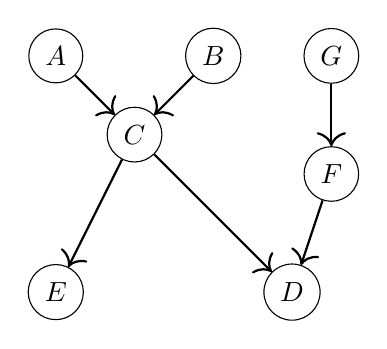
\begin{tikzpicture}
            \node[circle, draw] at (0, 3)   (a) {$A$};
            \node[circle, draw] at (1, 2)   (c) {$C$};
            \node[circle, draw] at (2, 3)   (b) {$B$};
            \node[circle, draw] at (3, 0)   (d) {$D$};
            \node[circle, draw] at (0, 0)   (e) {$E$};
            \node[circle, draw] at (3.5, 1.5)   (f) {$F$};
            \node[circle, draw] at (3.5, 3)   (g) {$G$};
            
            \draw [-{To[scale=1.5]}, thick] (a) -- (c);
            \draw [-{To[scale=1.5]}, thick] (b) -- (c);
            \draw [-{To[scale=1.5]}, thick] (c) -- (e);
            \draw [-{To[scale=1.5]}, thick] (c) -- (d);
            \draw [-{To[scale=1.5]}, thick] (f) -- (d);
            \draw [-{To[scale=1.5]}, thick] (g) -- (f);
        \end{tikzpicture} 
        &
        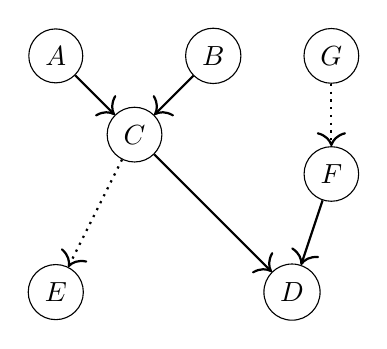
\begin{tikzpicture}
            \node[circle, draw] at (0, 3)   (a) {$A$};
            \node[circle, draw] at (1, 2)   (c) {$C$};
            \node[circle, draw] at (2, 3)   (b) {$B$};
            \node[circle, draw] at (3, 0)   (d) {$D$};
            \node[circle, draw] at (0, 0)   (e) {$E$};
            \node[circle, draw] at (3.5, 1.5)   (f) {$F$};
            \node[circle, draw] at (3.5, 3)   (g) {$G$};
            
            \draw [-{To[scale=1.5]}, thick] (a) -- (c);
            \draw [-{To[scale=1.5]}, thick] (b) -- (c);
            \draw [-{To[scale=1.5]}, thick, dotted] (c) -- (e);
            \draw [-{To[scale=1.5]}, thick] (c) -- (d);
            \draw [-{To[scale=1.5]}, thick] (f) -- (d);
            \draw [-{To[scale=1.5]}, thick, dotted] (g) -- (f);
        \end{tikzpicture}\\
        (a) & (b)\\
    \end{tabular}
    \caption{(a) represents a typical DAG construction. (b) denotes the representation of (a) where the edges that are not in an immortality, are dotted. }
    \label{fig:mk}
\end{figure}

\newpage
\section{Probabilistic Graphical Models}

Bayesian networks fall under the more general umbrella of \textbf{Graphical Models} (GMs), in which independence/dependence relationships are depicted. Each class of GM is a particular union of graph and probability constructs and details the form of independence assumptions presented. 

\noindent The main process for using probabilistic graphical models can be formulated in two parts. 
\begin{enumerate}
    \item \textbf{Modeling}: After identifying all potentially relevant variables in the problem environment, our task is to describe how these variables can interact. This is achieved using structural assumptions about the form of the joint probability distribution of all variables, in which independence assumptions are made. Each class of graphical model corresponds to a factorisation property of the joint probability distribution. 
    \item \textbf{Inference}: Once the basic assumptions regarding how the variables interact with each other is formed, all questions of interest are answered by performing inference on the distribution. The use of accurate inference algorithms with a particular GM is key here, as some algorithms are not a computationally trivial step to perform. 
\end{enumerate}

\subsection{Markov Networks}

In Bayesian networks, we rely on the joint probability distribution being a factorisation in which the factors are each a distribution in itself. \textbf{Markov Networks}~(MNs) define this factorisation in terms \textbf{potential functions} on maximal cliques in an undirected graph.
\\
\begin{theorem}
    \textbf{Clique}. Given an undirected graph, a clique is a fully connected subset of nodes. All members of the clique are \textbf{neighbours}. For a \textit{maximal clique}, there is no larger clique that contains the clique. 
\end{theorem}

\noindent For example, consider the graph in figure~\ref{fig:clique}. While the subset of nodes $\{A, B, C\}$ are fully connected and neighbours of each other, this subset is a non-maximal clique, as there is a clique that is larger than this clique, i.e., $\{A, B, C, D\}$. A non-maximal clique is often called a \textbf{cliquo}. The graph has two maximal cliques in total, $C_1 = \{A, B, C, D\}$ and $C_2 = \{B, C, E\}$. 

\begin{figure}[H]
    \centering
    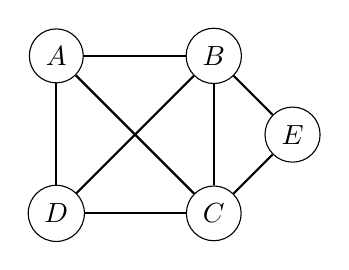
\begin{tikzpicture}
        \node[circle, draw] at (0, 2)   (a) {$A$};
        \node[circle, draw] at (2, 2)   (b) {$B$};
        \node[circle, draw] at (0, 0)   (d) {$D$};
        \node[circle, draw] at (2, 0)   (c) {$C$};
        \node[circle, draw] at (3, 1)   (e) {$E$};
        
        \draw [thick] (a) -- (b);\draw [thick] (a) -- (c);\draw [thick] (a) -- (d);
        \draw [thick] (b) -- (d);\draw [thick] (b) -- (c);\draw [thick] (b) -- (e);
        \draw [thick] (c) -- (e);\draw [thick] (c) -- (d);
    \end{tikzpicture}
    \caption{Example of an undirected graph, in which there are two maximal cliques, i.e., $C_1 = \{A, B, C, D\}$ and $C_2 = \{B, C, E\}$.}
    \label{fig:clique}
\end{figure}

\begin{theorem}
    \textbf{Potential}. A potential $\phi(x)$ is a non-negative function of the variable $x$, i.e., $\phi(x) \geq 0$. A joint potential $\phi(x_1, \dots, x_N)$ is a non-negative function of the set of variables. A distribution is a special case of a potential satisfying normalisation, i.e., $\sum_x \phi(x) = 1$. This holds similarly for continuous variables with summation replaced by integration. 
\end{theorem}

\begin{theorem}
    \textbf{Markov Network.} For a set of variables $\mathcal{X} = \{x_1, \dots, x_N\}$, a Markov network is defined as a product of potentials on subsets of the variables $\mathcal{X}_c \subseteq \mathcal{X}$:
    $$
        p(x_1, \dots, x_N) = \frac{1}{Z} \prod_{c=1}^C \phi_c (\mathcal{X}_c) .
    $$
    The constant $Z$ ensures that the distribution is normalised. Graphically, this is represented by an undirected graph $G$ with $\mathcal{X}_c, c = 1, \dots, C$ being the maximal cliques of $G$. If the clique potentials are strictly positive, this is called a \textit{Gibbs distribution}. 
\end{theorem}

\noindent As an example, consider a simple undirected graph of the form $A - C - B$, which has two maximal cliques, i.e., $\{A, C\}$ and $\{B, C\}$. On these sets of variables, we can define a \textit{potential function}, which maps the states of these sets of variables to some positive 'weight'. This weight may or may not be a probability. Suppose the potentials are as follows.
\begin{align*}
    &\phi_{AC}(A, C) &= 1           \qquad\qquad\qquad &&&\phi_{BC}(B, C) &= 1 \\
    &\phi_{AC}(\neg A, C) &= 0      \qquad\qquad\qquad &&&\phi_{BC}(\neg B, C) &= 1 \\
    &\phi_{AC}(A, \neg C) &= 2      \qquad\qquad\qquad &&&\phi_{BC}(B, \neg C) &= 2 \\
    &\phi_{AC}(\neg A, \neg C) &= 1 \qquad\qquad\qquad &&&\phi_{BC}(\neg B, \neg C) &= 1
\end{align*}
\noindent The joint probability is then defined as:
$$
    p(A, B, C) = \frac{1}{Z} \phi_{AC}(A, C)\phi_{BC}(B, C)
$$
where $Z$ is the normalisation constant. The full distribution is then as follows.
\begin{table}[H]
    \centering
    \begin{tabular}{|ccc|c|}
        \hline
        $A$ & $B$ & $C$ & $ \phi_{AC}(A, C)\phi_{BC}(B, C)$ \\ \hline
        0 & 0 & 0 & 1 \\
        0 & 0 & 1 & 0 \\
        0 & 1 & 0 & 2 \\
        0 & 1 & 1 & 0 \\
        1 & 0 & 0 & 2 \\
        1 & 0 & 1 & 1 \\
        1 & 1 & 0 & 4 \\
        1 & 1 & 1 & 1 \\\hline
    \end{tabular}
\end{table}

\noindent From this table, we can compute the normalisation constant $Z$:
$$
    Z = \sum_{A, B, C} \phi_{AC}(A, C)\phi_{BC}(B, C) = 1+0+2+0+2+1+4+1 = 11
$$
\noindent Inference is now trivial. For instance, $p(\neg A, B, \neg C) = \frac{2}{11}$ or $p(\neg A, B, C) = \frac{0}{11} = 0$.

\subsubsection{Pairwise Markov networks}

In the special case that the graph contains cliques of only size 2, the distribution is called a \textbf{pairwise Markov network}, with potentials defined on each link between variables. Whilst an MN is formally defined on maximal cliques, in practice, authors often use the term to refer to non-maximal cliques. 

\begin{wrapfigure}{o}{0.2\textwidth}
    \vspace{-20pt}
    \begin{center}
        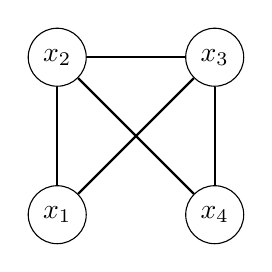
\begin{tikzpicture}
            \node[circle, draw] at (0, 0)   (x1) {$x_1$};
            \node[circle, draw] at (0, 2)   (x2) {$x_2$};
            \node[circle, draw] at (2, 2)   (x3) {$x_3$};
            \node[circle, draw] at (2, 0)   (x4) {$x_4$};

            \draw [thick] (x1) -- (x2);\draw [thick] (x1) -- (x3);
            \draw [thick] (x2) -- (x4);\draw [thick] (x2) -- (x3);
            \draw [thick] (x3) -- (x4);
        \end{tikzpicture}
    \end{center}
\end{wrapfigure}

Consider for example the graph on the right that has two maximal cliques, $\{x_1, x_2, x_3\}$ and $\{x_2, x_3, x_4\}$. The graph describes the distribution $p(x_1, x_2, x_3, x_4) = \frac{1}{Z} \phi(x_1, x_2, x_3)\phi(x_2, x_3, x_4)$. However, in a pairwise Markov network, the potentials are assumed to be over pairs of two cliques. This results in the non-maximal cliques, $\{x_1, x_2\}, \{x_1, x_3\}, \{x_2, x_4\}, \{x_2, x_3\}, \{x_3, x_4\}$. The distribution then becomes 
$$
    p(x_1, x_2, x_3, x_4) = \frac{1}{Z} \phi(x_1, x_2)\phi(x_1, x_3)\phi(x_2, x_4)\phi(x_2, x_3)\phi(x_3, x_4) .
$$

\subsubsection{Markov properties}

The separation criterion, sometimes called \textbf{U-separation}, for Markov networks is simpler than for Bayesian networks, due to the fact that there are no colliders. Informally, a path between nodes $A$ and $B$ is blocked if and only if there is an observed node $C$ on the path. 
\\
\begin{theorem}
    \textbf{Global Markov property and U-separation}. 
    \\
    A subset $\mathcal{S}$ separates a subset $\mathcal{A}$ from a subset $\mathcal{B}$ if every path from any member of $\mathcal{A}$ to any member of $\mathcal{B}$ passes through $\mathcal{S}$. If there is no path from a member of $\mathcal{A}$ to a member of $\mathcal{B}$, then $\mathcal{A}$ is separated from $\mathcal{B}$. 
    \\\\
    The \textbf{global Markov property} states that for disjoint sets of variables, $(\mathcal{A}, \mathcal{B}, \mathcal{S})$, where $\mathcal{S}$ separates $\mathcal{A}$ from $\mathcal{B}$ in $G$, then $\mathcal{A} \indep \mathcal{B} \,|\, \mathcal{S}$.
\end{theorem}

\noindent To determine whether the conditional independence statement $\mathcal{A} \indep \mathcal{B} \,|\, \mathcal{S}$ is true, we simply remove all links that neighbour the set of variables $\mathcal{S}$. If there is no path from any member of $\mathcal{A}$ to any member of $\mathcal{B}$, then $\mathcal{A} \indep \mathcal{B} \,|\, \mathcal{S}$ is true. 

As an example, consider the left Markov network of figure~\ref{fig:MN}, in which we can graphically observe that $x_1$ is independent of $x_7$ conditioned on $x_4$, i.e., $x_1 \indep x_7 \,|\, x_4$. The reason for this observation is trivial if we remove all edges attached to $x_4$, then there is no path from $x_1$ to $x_7$, as can be seen in the right graph.  

\begin{figure}[H]
    \centering
    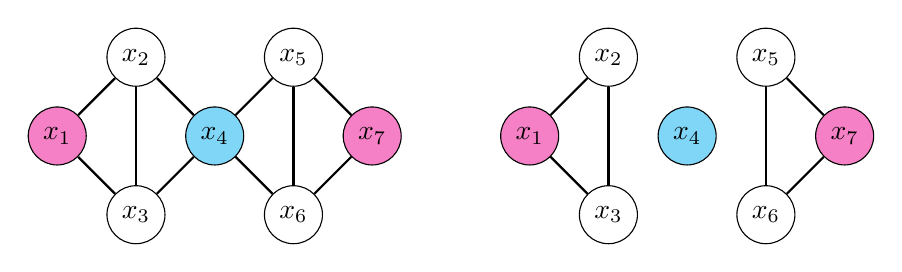
\begin{tikzpicture}
        \node[circle, draw, fill=magenta!50] at (0, 1)   (x1) {$x_1$};
        \node[circle, draw] at (1, 2)   (x2) {$x_2$};
        \node[circle, draw] at (1, 0)   (x3) {$x_3$};
        \node[circle, draw, fill=cyan!50] at (2, 1)   (x4) {$x_4$};
        \node[circle, draw] at (3, 2)   (x5) {$x_5$};
        \node[circle, draw] at (3, 0)   (x6) {$x_6$};
        \node[circle, draw, fill=magenta!50] at (4, 1)   (x7) {$x_7$};

        \draw [thick] (x1) -- (x2);\draw [thick] (x1) -- (x3);
        \draw [thick] (x2) -- (x3);\draw [thick] (x2) -- (x4);
        \draw [thick] (x3) -- (x4);
        \draw [thick] (x4) -- (x5);\draw [thick] (x4) -- (x6);
        \draw [thick] (x5) -- (x6);\draw [thick] (x5) -- (x7);
        \draw [thick] (x6) -- (x7);

        \node[circle, draw, fill=magenta!50] at (6, 1)   (x1_) {$x_1$};
        \node[circle, draw] at (7, 2)   (x2_) {$x_2$};
        \node[circle, draw] at (7, 0)   (x3_) {$x_3$};
        \node[circle, draw, fill=cyan!50] at (8, 1)   (x4_) {$x_4$};
        \node[circle, draw] at (9, 2)   (x5_) {$x_5$};
        \node[circle, draw] at (9, 0)   (x6_) {$x_6$};
        \node[circle, draw, fill=magenta!50] at (10, 1)   (x7_) {$x_7$};

        \draw [thick] (x1_) -- (x2_);
        \draw [thick] (x1_) -- (x3_);
        \draw [thick] (x2_) -- (x3_);
        \draw [thick] (x5_) -- (x6_);
        \draw [thick] (x5_) -- (x7_);
        \draw [thick] (x6_) -- (x7_);
    \end{tikzpicture}
    \caption{Markov network in which $x_1 \indep x_7 \giv x_4$ is depicted. The right Markov network shows the structure conditioned on $x_4$.}
    \label{fig:MN}
\end{figure}

\noindent We can also determine the conditional independence statement $x_1 \indep x_7 \,|\, x_4$ mathematically. There are 4 cliques, and thus, there are 4 potential functions,\\ $\phi(x_1, x_2, x_3), \phi(x_2, x_3, x_4), \phi(x_4, x_5, x_6), \phi(x_5, x_6, x_7)$.  
\begin{align*}
    p(x_1, x_7 \,|\, x_4) &\propto \sum_{x_2, x_3, x_5, x_6} p(x_1, x_2, x_3, x_4, x_5, x_6, x_7) \\
    &= \sum_{x_2, x_3, x_5, x_6} \phi(x_1, x_2, x_3)\phi(x_2, x_3, x_4)\phi(x_4, x_5, x_6)\phi(x_5, x_6, x_7) \\ 
    &= \left( \sum_{x_2, x_3} \phi(x_1, x_2, x_3)\phi(x_2, x_3, x_4) \right) \left( \sum_{x_5, x_6} \phi(x_4, x_5, x_6)\phi(x_5, x_6, x_7) \right) \\ 
    &= p(x_1 \,|\, x_4) p(x_7 \,|\, x_4)
\end{align*}

\subsection{Chain Graphs}

Chain graphs (CGs) contain both directed and undirected links between nodes. CGs contain chain components, which identify the region of undirected nodes. Bayesian networks are chain graphs in which the chain components are singletons. In other words, each connected component consists of a single node. Markov networks, on the other hand, are chain graphs in which there is a single chain component that covers every node in the graph. 
\\
\begin{theorem}
    \textbf{Chain Component}. To obtain the chain components of graph $G$, follow the following steps:
    \begin{enumerate}
        \item Construct a new graph $G'$ with \textbf{directed} edges removed from $G$. 
        \item Identify each chain component as the connected components in $G'$.
    \end{enumerate}
\end{theorem}

\begin{figure}[H]
    \centering
    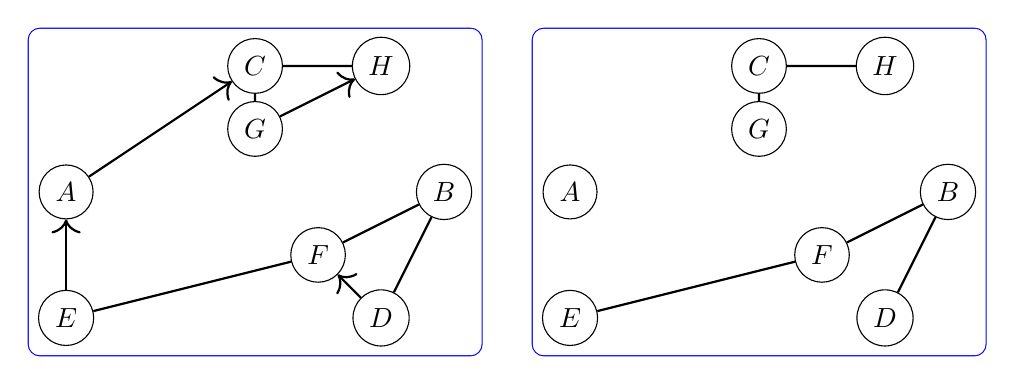
\begin{tikzpicture}[scale=.8]
        \node[circle, draw] at (0, 2)   (a) {$A$};
        \node[circle, draw] at (6, 2)   (b) {$B$};
        \node[circle, draw] at (3, 4)   (c) {$C$};
        \node[circle, draw] at (5, 0)   (d) {$D$};
        \node[circle, draw] at (0, 0)   (e) {$E$};
        \node[circle, draw] at (4, 1)   (f) {$F$};
        \node[circle, draw] at (3, 3)   (g) {$G$};
        \node[circle, draw] at (5, 4)   (h) {$H$};

        \draw [thick] (f) -- (b);
        \draw [thick] (b) -- (d);
        \draw [thick] (f) -- (e);
        \draw [thick] (c) -- (g);
        \draw [thick] (c) -- (h);
        \draw [-{To[scale=1.5]}, thick] (d) -- (f);
        \draw [-{To[scale=1.5]}, thick] (e) -- (a);
        \draw [-{To[scale=1.5]}, thick] (a) -- (c);
        \draw [-{To[scale=1.5]}, thick] (g) -- (h);

        \node[circle, draw] at (8, 2)   (a_) {$A$};
        \node[circle, draw] at (14, 2)   (b_) {$B$};
        \node[circle, draw] at (11, 4)   (c_) {$C$};
        \node[circle, draw] at (13, 0)   (d_) {$D$};
        \node[circle, draw] at (8, 0)   (e_) {$E$};
        \node[circle, draw] at (12, 1)   (f_) {$F$};
        \node[circle, draw] at (11, 3)   (g_) {$G$};
        \node[circle, draw] at (13, 4)   (h_) {$H$};

        \draw [thick] (f_) -- (b_);
        \draw [thick] (b_) -- (d_);
        \draw [thick] (f_) -- (e_);
        \draw [thick] (c_) -- (g_);
        \draw [thick] (c_) -- (h_);

        \pgfdeclarelayer{bg}
        \pgfsetlayers{bg,main}
        \begin{pgfonlayer}{bg}
             \node (box) [draw=blue,line width=.8pt,rounded corners,fit = (e) (c) (b)] {};
             \node (box) [fill=white,rounded corners,fit = (e) (c) (b)] {};
             \node (box) [draw=blue,line width=.8pt,rounded corners,fit = (e_) (c_) (b_)] {};
             \node (box) [fill=white,rounded corners,fit = (e_) (c_) (b_)] {};
        \end{pgfonlayer}
    \end{tikzpicture}
    \caption{Example of the identification of the chain components in a chain graph. After removing the directed edges from the left graph, we are left with the connected components in the right graph. The identified chain components are thus $\{A\}, \{ C, G, H\}, \{ E, F, B, D\}$.}
    \label{fig:CG_example}
\end{figure}

\begin{theorem}
    \textbf{Chain graph distribution.} The distribution associated with a chain graph $G$ is found by first identifying the chain components $\tau$. Then
    $$
        p(x) = \prod_{\tau} p(\mathcal{X}_\tau \,|\, \text{pa}(\mathcal{X}_\tau))
    $$
    where $p(\mathcal{X}_\tau \,|\, \text{pa}(\mathcal{X}_\tau))$ is proportional to
    $$
        p(\mathcal{X}_\tau \,|\, \text{pa}(\mathcal{X}_\tau)) \propto \prod_{c \in C_\tau} \phi(\mathcal{X}_{C_\tau})
    $$
    where $C_\tau$ denotes the union of the cliques in component $\tau$ together with the moralised parental components of $\tau$, with $\phi$ being the associated functions defined on each clique. The proportionality factor is determined implicitly by the constraint that the distribution sums to 1.  
\end{theorem}

\noindent Compared to Bayesian networks or Markov networks, Chain graphs are more expressive of conditional independence statements. As an example consider the following chain graph in figure~\ref{fig:CG}, in which we can express the conditional independence statements $a \indep b \,\,|\,\, \emptyset$ and $d \indep e \,\,|\,\, \{c, f\}$, whereas a directed graph could not express both these statements.

\begin{figure}[H]
    \centering
    \begin{tabular}{@{}ccc@{}}
        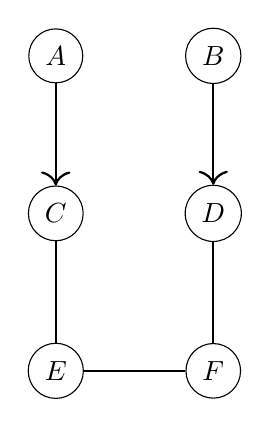
\begin{tikzpicture}
            \node[circle, draw] at (0, 4)   (a) {$A$};
            \node[circle, draw] at (2, 4)   (b) {$B$};
            \node[circle, draw] at (0, 2)   (c) {$C$};
            \node[circle, draw] at (2, 2)   (d) {$D$};
            \node[circle, draw] at (0, 0)   (e) {$E$};
            \node[circle, draw] at (2, 0)   (f) {$F$};
    
            \draw [thick] (c) -- (e);
            \draw [thick] (e) -- (f);
            \draw [thick] (f) -- (d);
            \draw [-{To[scale=1.5]}, thick] (a) -- (c);
            \draw [-{To[scale=1.5]}, thick] (b) -- (d);
        \end{tikzpicture}
        &
        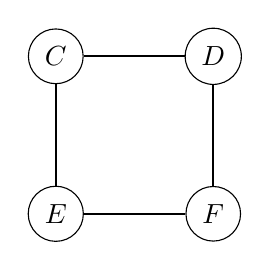
\begin{tikzpicture}
            \node[circle, draw] at (0, 2)   (c) {$C$};
            \node[circle, draw] at (2, 2)   (d) {$D$};
            \node[circle, draw] at (0, 0)   (e) {$E$};
            \node[circle, draw] at (2, 0)   (f) {$F$};
    
            \draw [thick] (c) -- (e);
            \draw [thick] (e) -- (f);
            \draw [thick] (f) -- (d);
            \draw [thick] (c) -- (d);
        \end{tikzpicture}
        &
        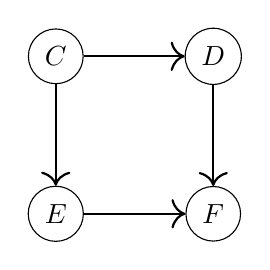
\begin{tikzpicture}
            \node[circle, draw] at (0, 2)   (c) {$C$};
            \node[circle, draw] at (2, 2)   (d) {$D$};
            \node[circle, draw] at (0, 0)   (e) {$E$};
            \node[circle, draw] at (2, 0)   (f) {$F$};
    
            \draw [-{To[scale=1.5]}, thick] (c) -- (e);
            \draw [-{To[scale=1.5]}, thick] (c) -- (d);
            \draw [-{To[scale=1.5]}, thick] (d) -- (f);
            \draw [-{To[scale=1.5]}, thick] (e) -- (f);
        \end{tikzpicture} \\ 
        (a) & (b) & (c)
    \end{tabular}
    \caption{The chain graph (a) is able to express the conditional independence statements $a \indep b \,\,|\,\, \emptyset$ and $d \indep e \,\,|\,\, \{c, f\}$, which are not possible to both express in a Bayesian network or a Markov network. (b) denotes the marginal distribution $p(c, d, e, f)$, which is a 4-cycle. Any DAG on a 4-cycle must contain a collider, as in (c), which expresses a different set of conditional independence statements than (b).}
    \label{fig:CG}
\end{figure}

\subsubsection{c-separation}

\begin{theorem}
    \textbf{c-separation.} We say that a set of variables $X$ is c-separated from a set of variables $Y$ by a set of variables $Z$, and write $X \indep Y \,|\, Z$ if and only if every \textbf{path} between $X$ and $Y$ is \textbf{intercepted} by $Z$. 
    \\
    \\
    Because we are dealing with directed and undirected edges, it is not sufficient to only consider \textit{trails}. In other words, it is not sufficient to only consider walks in which all edges are \textit{distinct}. 
\end{theorem}

\noindent To define the term \textbf{intercepted}, we first need to introduce the concept of \textbf{section}, which is the maximal undirected subpath $c_i - \dots - c_j$ of a path. In the following chain graph example, a possible path is $a \rightarrow c - d - c - d \leftarrow b$, which contains 3 distinct sections, i.e., $a, c - d - c - d$, $b$.

\begin{center}
    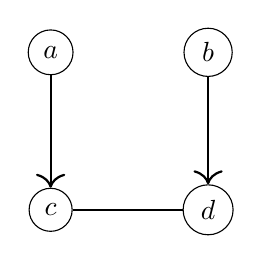
\begin{tikzpicture}
        \node[circle, draw] at (0, 2)   (a) {$a$};
        \node[circle, draw] at (2, 2)   (b) {$b$};
        \node[circle, draw] at (0, 0)   (c) {$c$};
        \node[circle, draw] at (2, 0)   (d) {$d$};

        \draw [thick] (c) -- (d);
        \draw [-{To[scale=1.5]}, thick] (a) -- (c);
        \draw [-{To[scale=1.5]}, thick] (b) -- (d);
    \end{tikzpicture}
\end{center}

\begin{theorem}
    \textbf{Collider section.} A section $c_i - \dots - c_j$ is a \textbf{collider section} if the path contains $c_{i-1} \rightarrow c_i - \dots - c_j \leftarrow c_{j+1}$. 
    
    \begin{center}
        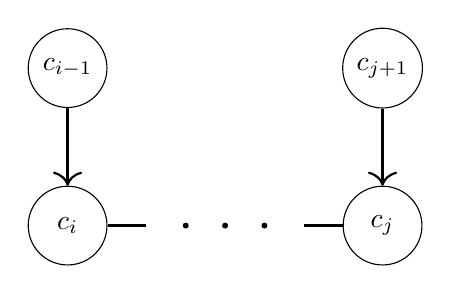
\begin{tikzpicture}
            \node[circle, draw, minimum size=1cm] at (0, 2)   (c_i1) {$c_{i-1}$};
            \node[circle, draw, minimum size=1cm] at (0, 0)   (c_i) {$c_i$};
            \node[circle, draw, minimum size=1cm] at (4, 0)   (c_j) {$c_j$};
            \node[circle, draw, minimum size=1cm] at (4, 2)   (c_j1) {$c_{j+1}$};
    
            \draw [thick] (c_i) -- (1, 0);
            \draw [thick] (c_j) -- (3, 0);
            \draw[black,fill=black] (1.5,0) circle (.2ex);
            \draw[black,fill=black] (2,0) circle (.2ex);
            \draw[black,fill=black] (2.5,0) circle (.2ex);
            
            \draw [-{To[scale=1.5]}, thick] (c_i1) -- (c_i);
            \draw [-{To[scale=1.5]}, thick] (c_j1) -- (c_j);
        \end{tikzpicture}
    \end{center}
\end{theorem}


\noindent Thus, in the example, $c - d - c - d$ is a collider section. A path is \textbf{not intercepted} by $Z$, i.e., is \textbf{superactive}, if 
\begin{itemize}
    \item[-] every collider section contains a node of $Z$; \textit{and}
    \item[-] every other section is outside $Z$.
\end{itemize}

\noindent Alternatively, we can define when a path is intercepted by $Z$, i.e., is blocked, if
\begin{itemize}
    \item[-] there is a collider section and there is no element in the collider section that is also in $Z$; \textit{or}
    \item[-] there is a section that is not a collider section and contains an element that is also in $Z$.
\end{itemize}

\noindent Analogously to d-separation, we can also construct the 4 possibilities given a triplet of sections, $A, B, C$ as follows. In the case that the conditioning set is empty, i.e., $A \indep B \,|\, C$, where $C = \emptyset$:
\begin{align*}
    & A \rightarrow c_i - \dots - c_j \rightarrow B \implies \text{Active}\\
    & A \leftarrow c_i - \dots - c_j \leftarrow B \implies \text{Active} \\
    & A \leftarrow c_i - \dots - c_j \rightarrow B \implies \text{Active}\\
    & A \rightarrow c_i - \dots - c_j \leftarrow B\implies \text{Inactive}
\end{align*}
\noindent And in the case where the conditioning set is non-empty, i.e., $A \indep B \,|\, C$, where $C = c_k$, $i \leq k \leq j$:
\begin{align*}
    & A \rightarrow c_i - \dots - c_j \rightarrow B \implies \text{Inactive}\\
    & A \leftarrow c_i - \dots - c_j \leftarrow B \implies \text{Inactive} \\
    & A \leftarrow c_i - \dots - c_j \rightarrow B \implies \text{Inactive}\\
    & A \rightarrow c_i - \dots - c_j \leftarrow B\implies \text{Active}
\end{align*}

\noindent To test the c-separation criterion on a given conditional independence statement, the following algorithm can be applied. Given a conditional independence statement $A \indep B \,|\, C$, first, construct the \textbf{upwardly closed subgraph} of the nodes $A \cup B \cup C$. The upwardly closed subgraph of a set of nodes $Z$ are the nodes in $Z$, the boundaries of $Z$, and the boundaries of the nodes in the boundaries of $Z$. This definition holds recursively. The boundary of a node $X$ is the union of the parents of $X$ and the neighbours of $X$, i.e., $\text{bdr}(X) = \text{pa}(X) \cup \text{ngb}(X)$. As an example consider the following chain graph in figure~\ref{fig:csep}. 

\begin{figure}[H]
    \centering
    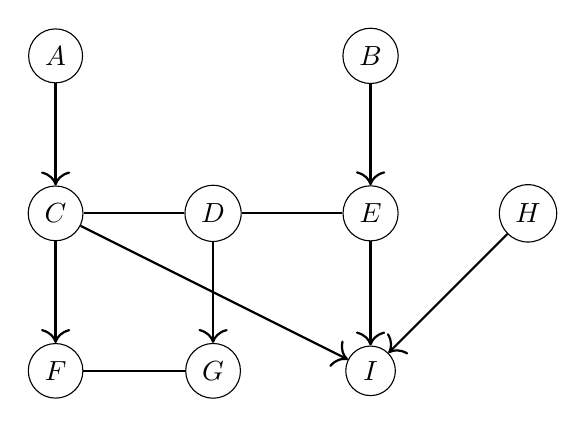
\begin{tikzpicture}
        \node[circle, draw] at (0, 4)   (a) {$A$};
        \node[circle, draw] at (4, 4)   (b) {$B$};
        \node[circle, draw] at (0, 2)   (c) {$C$};
        \node[circle, draw] at (2, 2)   (d) {$D$};
        \node[circle, draw] at (4, 2)   (e) {$E$};
        \node[circle, draw] at (0, 0)   (f) {$F$};
        \node[circle, draw] at (2, 0)   (g) {$G$};
        \node[circle, draw] at (6, 2)   (h) {$H$};
        \node[circle, draw] at (4, 0)   (i) {$I$};

        \draw [thick] (c) -- (d) -- (e);
        \draw [thick] (f) -- (g);
        \draw [-{To[scale=1.5]}, thick] (a) -- (c);
        \draw [-{To[scale=1.5]}, thick] (c) -- (f);
        \draw [-{To[scale=1.5]}, thick] (d) -- (g);
        \draw [-{To[scale=1.5]}, thick] (c) -- (i);
        \draw [-{To[scale=1.5]}, thick] (e) -- (i);
        \draw [-{To[scale=1.5]}, thick] (h) -- (i);
        \draw [-{To[scale=1.5]}, thick] (b) -- (e);
    \end{tikzpicture}
    \caption{Example chain graph to find the upwardly closed subgraph.}
    \label{fig:csep}
\end{figure}

\noindent To find the upwardly closed subgraph of the set $\{F\}$, first include $F$, then its neighbours, i.e., $G$, then its parents, i.e., $C$. Next, start again with the included nodes $G$ and $C$, and repeat. Figure~\ref{fig:csep_2} illustrates these steps.

\begin{figure}[H]
    \centering
    \begin{tabular}{@{}cc@{}}
        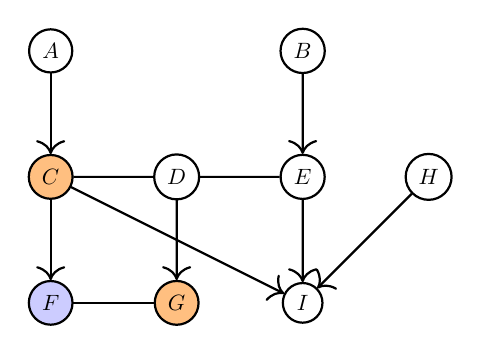
\begin{tikzpicture}[thick,scale=0.8, every node/.style={scale=0.8}]
            \node[circle, draw] at (0, 4)   (a) {$A$};
            \node[circle, draw] at (4, 4)   (b) {$B$};
            \node[circle, draw, fill=orange!50] at (0, 2)   (c) {$C$};
            \node[circle, draw] at (2, 2)   (d) {$D$};
            \node[circle, draw] at (4, 2)   (e) {$E$};
            \node[circle, draw, fill=blue!20] at (0, 0)   (f) {$F$};
            \node[circle, draw, fill=orange!50] at (2, 0)   (g) {$G$};
            \node[circle, draw] at (6, 2)   (h) {$H$};
            \node[circle, draw] at (4, 0)   (i) {$I$};
    
            \draw [thick] (c) -- (d) -- (e);
            \draw [thick] (f) -- (g);
            \draw [-{To[scale=1.5]}, thick] (a) -- (c);
            \draw [-{To[scale=1.5]}, thick] (c) -- (f);
            \draw [-{To[scale=1.5]}, thick] (d) -- (g);
            \draw [-{To[scale=1.5]}, thick] (c) -- (i);
            \draw [-{To[scale=1.5]}, thick] (e) -- (i);
            \draw [-{To[scale=1.5]}, thick] (h) -- (i);
            \draw [-{To[scale=1.5]}, thick] (b) -- (e);
        \end{tikzpicture}
        &
        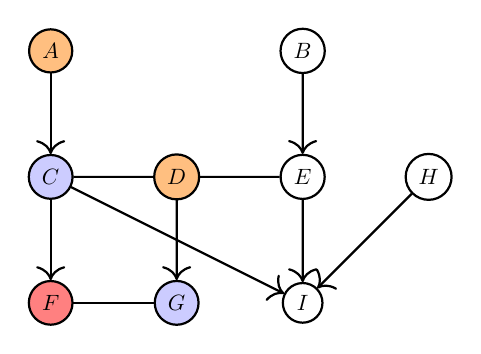
\begin{tikzpicture}[thick,scale=0.8, every node/.style={scale=0.8}]
            \node[circle, draw, fill=orange!50] at (0, 4)   (a) {$A$};
            \node[circle, draw] at (4, 4)   (b) {$B$};
            \node[circle, draw, fill=blue!20] at (0, 2)   (c) {$C$};
            \node[circle, draw, fill=orange!50] at (2, 2)   (d) {$D$};
            \node[circle, draw] at (4, 2)   (e) {$E$};
            \node[circle, draw, fill=red!50] at (0, 0)   (f) {$F$};
            \node[circle, draw, fill=blue!20] at (2, 0)   (g) {$G$};
            \node[circle, draw] at (6, 2)   (h) {$H$};
            \node[circle, draw] at (4, 0)   (i) {$I$};
    
            \draw [thick] (c) -- (d) -- (e);
            \draw [thick] (f) -- (g);
            \draw [-{To[scale=1.5]}, thick] (a) -- (c);
            \draw [-{To[scale=1.5]}, thick] (c) -- (f);
            \draw [-{To[scale=1.5]}, thick] (d) -- (g);
            \draw [-{To[scale=1.5]}, thick] (c) -- (i);
            \draw [-{To[scale=1.5]}, thick] (e) -- (i);
            \draw [-{To[scale=1.5]}, thick] (h) -- (i);
            \draw [-{To[scale=1.5]}, thick] (b) -- (e);
        \end{tikzpicture}\\
        (a) & (b) \\
        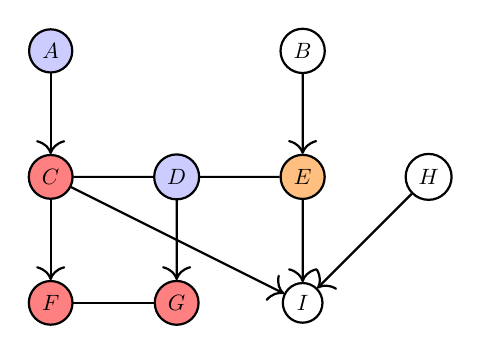
\begin{tikzpicture}[thick,scale=0.8, every node/.style={scale=0.8}]
            \node[circle, draw, fill=blue!20] at (0, 4)   (a) {$A$};
            \node[circle, draw] at (4, 4)   (b) {$B$};
            \node[circle, draw, fill=red!50] at (0, 2)   (c) {$C$};
            \node[circle, draw, fill=blue!20] at (2, 2)   (d) {$D$};
            \node[circle, draw, fill=orange!50] at (4, 2)   (e) {$E$};
            \node[circle, draw, fill=red!50] at (0, 0)   (f) {$F$};
            \node[circle, draw, fill=red!50] at (2, 0)   (g) {$G$};
            \node[circle, draw] at (6, 2)   (h) {$H$};
            \node[circle, draw] at (4, 0)   (i) {$I$};
    
            \draw [thick] (c) -- (d) -- (e);
            \draw [thick] (f) -- (g);
            \draw [-{To[scale=1.5]}, thick] (a) -- (c);
            \draw [-{To[scale=1.5]}, thick] (c) -- (f);
            \draw [-{To[scale=1.5]}, thick] (d) -- (g);
            \draw [-{To[scale=1.5]}, thick] (c) -- (i);
            \draw [-{To[scale=1.5]}, thick] (e) -- (i);
            \draw [-{To[scale=1.5]}, thick] (h) -- (i);
            \draw [-{To[scale=1.5]}, thick] (b) -- (e);
        \end{tikzpicture}
        &
        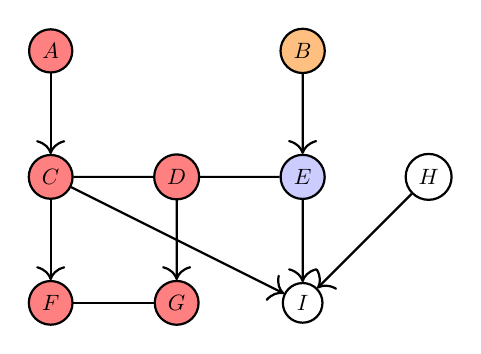
\begin{tikzpicture}[thick,scale=0.8, every node/.style={scale=0.8}]
            \node[circle, draw, fill=red!50] at (0, 4)   (a) {$A$};
            \node[circle, draw, fill=orange!50] at (4, 4)   (b) {$B$};
            \node[circle, draw, fill=red!50] at (0, 2)   (c) {$C$};
            \node[circle, draw, fill=red!50] at (2, 2)   (d) {$D$};
            \node[circle, draw, fill=blue!20] at (4, 2)   (e) {$E$};
            \node[circle, draw, fill=red!50] at (0, 0)   (f) {$F$};
            \node[circle, draw, fill=red!50] at (2, 0)   (g) {$G$};
            \node[circle, draw] at (6, 2)   (h) {$H$};
            \node[circle, draw] at (4, 0)   (i) {$I$};
    
            \draw [thick] (c) -- (d) -- (e);
            \draw [thick] (f) -- (g);
            \draw [-{To[scale=1.5]}, thick] (a) -- (c);
            \draw [-{To[scale=1.5]}, thick] (c) -- (f);
            \draw [-{To[scale=1.5]}, thick] (d) -- (g);
            \draw [-{To[scale=1.5]}, thick] (c) -- (i);
            \draw [-{To[scale=1.5]}, thick] (e) -- (i);
            \draw [-{To[scale=1.5]}, thick] (h) -- (i);
            \draw [-{To[scale=1.5]}, thick] (b) -- (e);
        \end{tikzpicture} \\ 
        (c) & (d)
    \end{tabular}
    \caption{(a) start with $F$ and include its neighbours and parents, i.e., $C$ and $G$. (b) start with $C$ and $G$, and include their neighbours and parents, i.e., $A$ and $D$. (c) start with $A$ and $D$, and include their neighbours and parents, i.e., $E$. (d) start with $E$ and include its neighbours and parents, i.e., $B$. The upwardly closed subgraph consists of nodes $\{A, C, F, G, D, E, B\}$. }
    \label{fig:csep_2}
\end{figure}

\noindent Having found the upwardly closed subgraph of the union $A \cup B \cup C$, the next step is to moralise the subgraph. The \textbf{moralised} counterpart of a (partially) directed acyclic graph is formed by adding undirected edges between all pairs of non-adjacent nodes that have a common child, and removing the direction of the edges from the subgraph. After moralisation of the subgraph, the subgraph is now an undirected graph, which is trivial to infer conditional independence on.  

As an example. Suppose we take the graph from figure~\ref{fig:csep} and want to know whether node $C$ is c-separated from node $E$ given $D, A$, i.e., $C \indep E \,|\, D, A$. Figure~\ref{fig:csep_ex} illustrates the steps.

\begin{figure}[H]
    \centering
    \begin{tabular}{@{}ccccc@{}}
        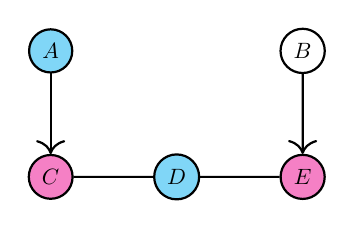
\begin{tikzpicture}[thick,scale=0.8, every node/.style={scale=0.8}]
            \node[circle, draw, fill=cyan!50] at (0, 4)   (a) {$A$};
            \node[circle, draw] at (4, 4)   (b) {$B$};
            \node[circle, draw, fill=magenta!50] at (0, 2)   (c) {$C$};
            \node[circle, draw, fill=cyan!50] at (2, 2)   (d) {$D$};
            \node[circle, draw, fill=magenta!50] at (4, 2)   (e) {$E$};
    
            \draw [thick] (c) -- (d) -- (e);
            \draw [-{To[scale=1.5]}, thick] (a) -- (c);
            \draw [-{To[scale=1.5]}, thick] (b) -- (e);
        \end{tikzpicture}
        &
        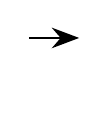
\begin{tikzpicture}[thick,scale=0.8, every node/.style={scale=0.8}]
            \draw [thick] (0, 0) -- (0, 0);
            \draw [-{Stealth[scale=1.5]}, thick] (0, 1) -- (.8, 1);
        \end{tikzpicture}
        &
        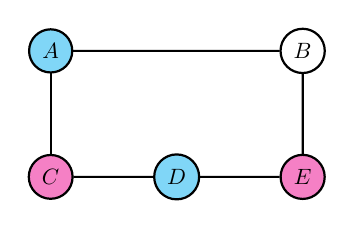
\begin{tikzpicture}[thick,scale=0.8, every node/.style={scale=0.8}]
            \node[circle, draw, fill=cyan!50] at (0, 4)   (a) {$A$};
            \node[circle, draw] at (4, 4)   (b) {$B$};
            \node[circle, draw, fill=magenta!50] at (0, 2)   (c) {$C$};
            \node[circle, draw, fill=cyan!50] at (2, 2)   (d) {$D$};
            \node[circle, draw, fill=magenta!50] at (4, 2)   (e) {$E$};
    
            \draw [thick] (c) -- (d) -- (e);
            \draw [thick] (a) -- (b);
            \draw [thick] (a) -- (c);
            \draw [thick] (b) -- (e);
        \end{tikzpicture}
        &
        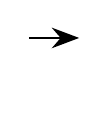
\begin{tikzpicture}[thick,scale=0.8, every node/.style={scale=0.8}]
            \draw [thick] (0, 0) -- (0, 0);
            \draw [-{Stealth[scale=1.5]}, thick] (0, 1) -- (.8, 1);
        \end{tikzpicture}
        &
        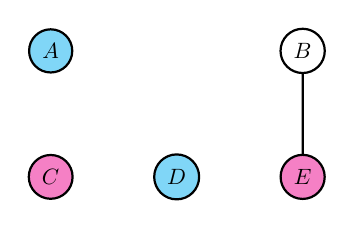
\begin{tikzpicture}[thick,scale=0.8, every node/.style={scale=0.8}]
            \node[circle, draw, fill=cyan!50] at (0, 4)   (a) {$A$};
            \node[circle, draw] at (4, 4)   (b) {$B$};
            \node[circle, draw, fill=magenta!50] at (0, 2)   (c) {$C$};
            \node[circle, draw, fill=cyan!50] at (2, 2)   (d) {$D$};
            \node[circle, draw, fill=magenta!50] at (4, 2)   (e) {$E$};
    
            \draw [thick] (b) -- (e);
        \end{tikzpicture}\\
        (a) & & (b) & & (c)\\
    \end{tabular}
    \caption{(a) denotes the upwardly closed subgraph of $C \cup E \cup \{D, A\}$. (b) denotes the moralised counterpart of (a), in which nodes $A$ and $B$ are connected because they have a common child in section $C - D - E$. (c) illustrates the effect of conditioning on $D, A$, by which there is no path from $C$ to $E$, i.e., $C$ is c-separated from $E$ given $D, A$. }
    \label{fig:csep_ex}
\end{figure}

\noindent As another example, consider the conditional independence statement $C \indep E \,|\, D, A, I$. Figure~\ref{fig:csep_ex2} illustrates the steps using c-separation.

\begin{figure}[H]
    \centering
    \begin{tabular}{@{}cc@{}}
        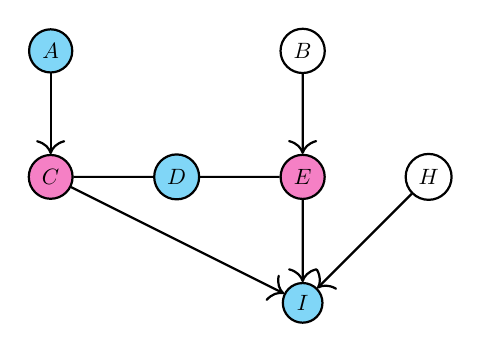
\begin{tikzpicture}[thick,scale=0.8, every node/.style={scale=0.8}]
            \node[circle, draw, fill=cyan!50] at (0, 4)   (a) {$A$};
            \node[circle, draw] at (4, 4)   (b) {$B$};
            \node[circle, draw, fill=magenta!50] at (0, 2)   (c) {$C$};
            \node[circle, draw, fill=cyan!50] at (2, 2)   (d) {$D$};
            \node[circle, draw, fill=magenta!50] at (4, 2)   (e) {$E$};
            \node[circle, draw] at (6, 2)   (h) {$H$};
            \node[circle, draw, fill=cyan!50] at (4, 0)   (i) {$I$};
    
            \draw [thick] (c) -- (d) -- (e);
            \draw [-{To[scale=1.5]}, thick] (a) -- (c);
            \draw [-{To[scale=1.5]}, thick] (c) -- (i);
            \draw [-{To[scale=1.5]}, thick] (e) -- (i);
            \draw [-{To[scale=1.5]}, thick] (h) -- (i);
            \draw [-{To[scale=1.5]}, thick] (b) -- (e);
        \end{tikzpicture}
        & \qquad\qquad
        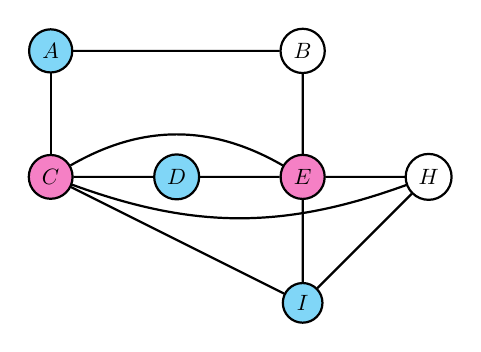
\begin{tikzpicture}[thick,scale=0.8, every node/.style={scale=0.8}]
            \node[circle, draw, fill=cyan!50] at (0, 4)   (a) {$A$};
            \node[circle, draw] at (4, 4)   (b) {$B$};
            \node[circle, draw, fill=magenta!50] at (0, 2)   (c) {$C$};
            \node[circle, draw, fill=cyan!50] at (2, 2)   (d) {$D$};
            \node[circle, draw, fill=magenta!50] at (4, 2)   (e) {$E$};
            \node[circle, draw] at (6, 2)   (h) {$H$};
            \node[circle, draw, fill=cyan!50] at (4, 0)   (i) {$I$};
    
            \draw [thick] (c) -- (d) -- (e);
            \draw [thick] (a) -- (b);
            \draw [thick] (a) -- (c);
            \draw [thick] (c) -- (i);
            \draw [thick] (e) -- (i);
            \draw [thick] (e) -- (h);
            \draw [thick] (h) -- (i);
            \draw [thick] (b) -- (e);
            \path[-] (c)  edge   [bend left=30]   node {} (e);
            \path[-] (c)  edge   [bend right=20]   node {} (h);
            % \draw [thick, bend right=20] (c) -- (e); \draw [thick, bend left=20] (c) -- (h);
        \end{tikzpicture}\\
        (a) &\qquad\qquad (b) \\ \\
        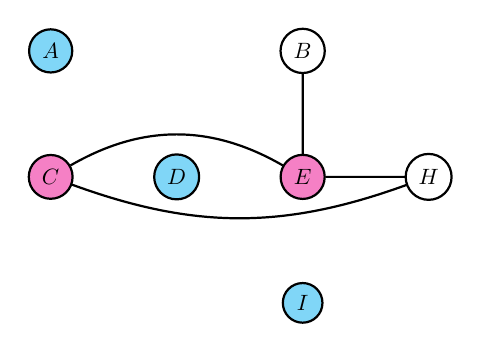
\begin{tikzpicture}[thick,scale=0.8, every node/.style={scale=0.8}]
            \node[circle, draw, fill=cyan!50] at (0, 4)   (a) {$A$};
            \node[circle, draw] at (4, 4)   (b) {$B$};
            \node[circle, draw, fill=magenta!50] at (0, 2)   (c) {$C$};
            \node[circle, draw, fill=cyan!50] at (2, 2)   (d) {$D$};
            \node[circle, draw, fill=magenta!50] at (4, 2)   (e) {$E$};
            \node[circle, draw] at (6, 2)   (h) {$H$};
            \node[circle, draw, fill=cyan!50] at (4, 0)   (i) {$I$};
            
            \draw [thick] (b) -- (e);
            \draw [thick] (h) -- (e);
            \path[-] (c)  edge   [bend left=30]   node {} (e);
            \path[-] (c)  edge   [bend right=20]   node {} (h);
        \end{tikzpicture}\\
        (c) & \\
    \end{tabular}
    \caption{(a) denotes the upwardly closed subgraph of $C \cup E \cup \{D, A, I\}$. (b) denotes the moralised counterpart of (a), in which nodes $A$ and $B$ are connected because they have a common child in section $C - D - E$, and $C, E, H$ are connected, because they have a common child in $I$. (c) illustrates the effect of conditioning on $D, A, I$, by which there is a path from $C$ to $E$, i.e., $C$ is not c-separated from $E$ given $D, A$.}
    \label{fig:csep_ex2}
\end{figure}

\subsection{Factor Graphs}

Factor graphs (FGs) are mainly used as part of inference algorithms. Zhang~\cite{Zhang2015DeepDiveAD} describes factor graphs as having two types of nodes. 
\begin{itemize}
    \item \textbf{Variables}, which can be either \textit{evidence variables} when their true value is known, or \textit{query variables} when their value should be predicted. 
    \item \textbf{Factors}, which define the relationship between variables in the graph. Each factor can be connected to many variables and comes with a \textbf{factor function} to define the relationship between these variables. 
\end{itemize}
\noindent We are typically not concerned with independencies in factor graphs. Any factorised distribution can be represented as a factor graph, which makes it an ideal representation for inference engines. They are typically not studied as a representation of independencies.
\\
\begin{theorem}
    \textbf{Factor graph.} Given a function 
    $$
        f(x_1, \dots, x_n) = \prod_i \psi_i(\mathcal{X}_i),
    $$
    the factor graph has a node (represented by a square) for each factor $\psi_i$, and a variables node (represented by a circle) for each variable $x_j$. for each $x_j \in \mathcal{X}_i$ an undirected link is made between factor $\psi_i$ and variable $x_j$. 
    \\\\
    When used to represent a distribution
    $$
        p(x_1, \dots, x_n) = \frac{1}{Z} \prod_i \psi_i(\mathcal{X}_i)
    $$
    a normalisation constant $Z = \sum_\mathcal{X} \prod_i \psi_i(\mathcal{X}_i)$ is assumed. 
    \\\\
    For a factor $\psi_i(\mathcal{X}_i)$, which is a conditional distribution of the form $p(x_i \,|\, \text{pa}(x_i))$, we may use directed links from the parents to the factor node, and directed links from the factor node to the child $x_i$. This has the same structure as an undirected FG, but preserves the information that the factors are distributions. 
\end{theorem}

\noindent Factor graphs are useful due to their ability to preserve more information than Markov networks, Bayesian networks, or chain graphs. BNs, MN, and CGs do not quantify the relationship between a pair of nodes, whereas factor graphs do by a variable 'weight' of the relationship. Consider the following FGs in figure~\ref{fig:FG}, which illustrate the various forms of FGs. 

\begin{figure}[H]
    \centering
    \begin{tabular}{@{}ccc@{}}
        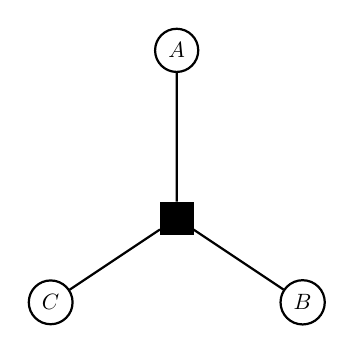
\begin{tikzpicture}[thick,scale=0.8, every node/.style={scale=0.8}]
            \node[circle, draw] at (2, 4)   (a) {$A$};
            \node[circle, draw] at (4, 0)   (b) {$B$};
            \node[circle, draw] at (0, 0)   (c) {$C$};
            \node[rectangle, draw, fill=black, minimum size=.5cm] at (2, 1.333)   (r) {};

            \draw [thick] (r) -- (a);
            \draw [thick] (r) -- (b);
            \draw [thick] (r) -- (c);
            
        \end{tikzpicture}
        &
        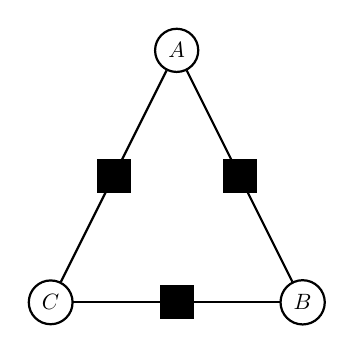
\begin{tikzpicture}[thick,scale=0.8, every node/.style={scale=0.8}]
            \node[circle, draw] at (2, 4)   (a) {$A$};
            \node[circle, draw] at (4, 0)   (b) {$B$};
            \node[circle, draw] at (0, 0)   (c) {$C$};
            \node[rectangle, draw, fill=black, minimum size=.5cm] at (3, 2)   (r1) {};
            \node[rectangle, draw, fill=black, minimum size=.5cm] at (1, 2)   (r2) {};
            \node[rectangle, draw, fill=black, minimum size=.5cm] at (2, 0)   (r3) {};

            \draw [thick] (a) -- (b);
            \draw [thick] (a) -- (c);
            \draw [thick] (b) -- (c);
        \end{tikzpicture}
        &
        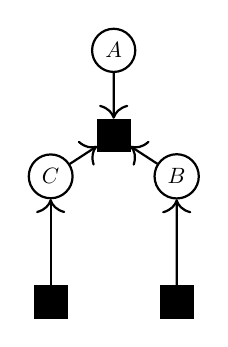
\begin{tikzpicture}[thick,scale=0.8, every node/.style={scale=0.8}]
            \node[circle, draw] at (1, 2)   (a) {$A$};
            \node[circle, draw] at (2, 0)   (b) {$B$};
            \node[circle, draw] at (0, 0)   (c) {$C$};
            \node[rectangle, draw, fill=black, minimum size=.5cm] at (1, .65)   (r) {};
            \node[rectangle, draw, fill=black, minimum size=.5cm] at (0, -2)   (rl) {};
            \node[rectangle, draw, fill=black, minimum size=.5cm] at (2, -2)   (rr) {};

            \draw [-{To[scale=1.5]}, thick] (a) -- (r);
            \draw [-{To[scale=1.5]}, thick] (b) -- (r);
            \draw [-{To[scale=1.5]}, thick] (c) -- (r);
            \draw [-{To[scale=1.5]}, thick] (rl) -- (c);
            \draw [-{To[scale=1.5]}, thick] (rr) -- (b);
        \end{tikzpicture}\\
        (a) & (b) & (c)\\
    \end{tabular}
    \caption{(a) illustrates an unfactored clique potential $\phi(a, b, c)$. (b) represents an unfactored clique potential with maximal cliques of 2, $\phi(a, b)\phi(b, c)\phi(a, c)$. (c) denotes a directed factor graph representation in which more information about the independence is preserved. A directed factor represents the term $p(\text{children} \,|\, \text{parents}$). }
    \label{fig:FG}
\end{figure}

\subsection{Expressiveness of probabilistic graphical models}

Directed distributions, such as BNs and CGs, can be represented as undirected distributions, such as MNs, by associating each normalised factor of the joint distribution with a potential function. The distribution $p(a \giv b)p(b \giv c)p(c)$ can be factored as $\phi(a, b)\phi(b, c)$, where $\phi(a, b) = p(a \giv b)$ and $\phi(b, c) = p(b \giv c)p(c)$, with $Z = 1$. Thus, every Bayesian network can be represented as some Markov network by identifying the factors in the distribution. 

However, consider the distribution $p(c \giv a, b) p(a) p(b)$, for which its Markov equivalent network contains additional links, which corresponds to the moralised directed graph. Therefore, information regarding independence will be lost when converting a directed graph into an undirected graph. In the aforementioned example, the Markov network of $p(c \giv a, b) p(a) p(b)$ is a single clique $\phi(a, b, c)$ from which it is not possible anymore to infer $a \indep b$. 

The graphical representation of a model may describe some list of conditional independence statements $\mathcal{L}_G$, whereas the probability distribution of a model also may describe some list of conditional independence statements $\mathcal{L}_P$. The relation between these sets, $\mathcal{L}_G, \mathcal{L}_P$, provides answers as to how consistent the dependence and independence statements in the graphical model are compared to the probability distribution. 
\\
\begin{theorem}
    \textbf{I-map, D-map, and P-map.} A graph is an \textit{independence map} (\textbf{I-map}) of a given distribution $P$ if every conditional independence statement that one can derive from the graph $G$ is true in the distribution $P$. That is
    $$
        \mathcal{X} \indep \mathcal{Y} \giv \mathcal{Z}_G \implies \mathcal{X} \indep \mathcal{Y} \giv \mathcal{Z}_P
    $$
    for all disjoint sets $\mathcal{X}, \mathcal{Y}, \mathcal{Z}$.
    \\
    A graph is a \textit{dependence map} (\textbf{D-map}) of a given distribution $P$ if every conditional independence statement that one can derive from $P$ is true in the graph $G$. That is
    $$
        \mathcal{X} \indep \mathcal{Y} \giv \mathcal{Z}_G \Longleftarrow \mathcal{X} \indep \mathcal{Y} \giv \mathcal{Z}_P
    $$
    for all disjoint sets $\mathcal{X}, \mathcal{Y}, \mathcal{Z}$. This is by contraposition equivalent to 
    $$
        \mathcal{X} \dep \mathcal{Y} \giv \mathcal{Z}_P \implies \mathcal{X} \dep \mathcal{Y} \giv \mathcal{Z}_G .
    $$
    \\
    A graph $G$ which is both I-map and D-map for $P$ is a \textit{perfect map} (\textbf{P-map}) and 
    $$
        \mathcal{X} \indep \mathcal{Y} \giv \mathcal{Z}_G \iff \mathcal{X} \indep \mathcal{Y} \giv \mathcal{Z}_P
    $$
    for all disjoint sets $\mathcal{X}, \mathcal{Y}, \mathcal{Z}$.
\end{theorem}

\noindent In other words, the relation between the list of conditional independence statements in $G$ and in $P$, denoted as $\mathcal{L}_G$ and $\mathcal{L}_P$, respectively, is the following:
\begin{align*}
    &\mathcal{L}_P \subseteq \mathcal{L}_G \qquad &&\mathcal{L}_P \text{ is a subset of } \mathcal{L}_G \qquad &\text{D-map}\\
    &\mathcal{L}_G \subseteq \mathcal{L}_P \qquad &&\mathcal{L}_G \text{ is a subset of } \mathcal{L}_P \qquad &\text{I-map}\\
    &\mathcal{L}_P = \mathcal{L}_G \qquad &&\mathcal{L}_P \text{ is equal to } \mathcal{L}_G \qquad &\text{P-map}
\end{align*}

\noindent As an example, consider the following distribution
$$
    p(x, y, z) = p(z \giv x, y)p(x)p(y)
$$
Which has a perfect map (P-map) $x \rightarrow z \leftarrow y$, as the list of conditional independence statements in both the distribution and the graph are equal, i.e., $\mathcal{L}_P = \mathcal{L}_G$. However, if we consider the undirected graph of the distribution, then $x, y, z$ are fully connected which makes $\mathcal{L}_G$ empty. There is no D-map in the undirected example because $\mathcal{L}_P$ is not a subset of $\mathcal{L}_G$. 

Given a factorisation of a distribution, for which we can trivially construct an I-map by following the dependencies of the conditional probability factors, it is possible to construct an I-map that is minimal. To do so, we need to determine if the various values of the conditional variables are equal to each other. For example, given the binary distribution $p(A \giv B, C) p(B \giv C) p(C) p(B)$, we can remove the link $B \rightarrow A$ iff $p(A \giv b, C) = p(A \giv \neg b, C)$ for all values of $A$ and $C$. 

\subsubsection{Example: directed and undirected I-maps}

\noindent As another example, consider the following joint distribution.
$$
    p(x_1, x_2, x_3, x_4, x_5) = p(x_1 \giv x_2, x_5) p(x_2 \giv x_3, x_4, x_5) p(x_3 \giv x_5, x_4) p(x_4) p(x_5)
$$
\noindent First, to construct an \textbf{undirected I-map} given this distribution, we can define the following potentials:
\begin{align*}
    \phi(x_1, x_2, x_5) &= p(x_1 \giv x_2, x_5) \\
    \phi(x_2, x_3, x_4, x_5) &= p(x_2 \giv x_3, x_4, x_5) p(x_3 \giv x_5, x_4) p(x_4) p(x_5)  
\end{align*}
\noindent These potentials represent the maximal cliques and can be represented in an undirected graph, i.e., Markov network, as seen in figure~\ref{fig:imap}a. To construct a \textbf{directed I-map} of the distribution, we can look at the distribution and simply built the Bayesian network by following the dependencies. This results in figure~\ref{fig:imap}b. 

% Finally, to construct the \textbf{minimal directed I-map}, we need to find the redundant edges and eliminate them from the graph. The result is illustrated in figure~\ref{fig:imap}c. The conditional independence statements leading to the elimination of the edges are $x_1 \indep x_5 \giv x_2$, $x_2 \indep x_5 \giv x_3$, and $x_2 \indep x_4 \giv x_3$. The reason why this I-map can be minimized is because $\mathcal{L}_G \subseteq \mathcal{L}_P$, i.e., the conditional independence statements derived from the $G$ are just a subset of the statements in $P$. 

\begin{figure}[H]
    \centering
    \begin{tabular}{@{}cc@{}}
        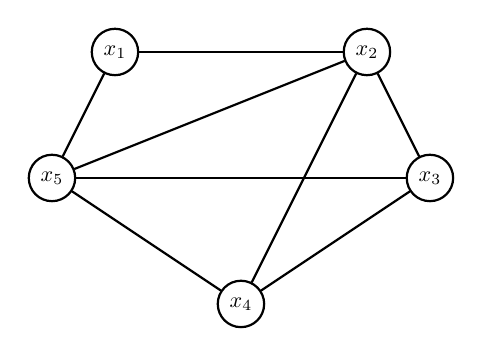
\begin{tikzpicture}[thick,scale=0.8, every node/.style={scale=0.8}]
            \node[circle, draw] at (-2, 4)   (x1) {$x_1$};
            \node[circle, draw] at (2, 4)   (x2) {$x_2$};
            \node[circle, draw] at (3, 2)   (x3) {$x_3$};
            \node[circle, draw] at (0, 0)   (x4) {$x_4$};
            \node[circle, draw] at (-3, 2)   (x5) {$x_5$};
        
            \draw [thick] (x1) -- (x2);
            \draw [thick] (x1) -- (x5);
            \draw [thick] (x2) -- (x5);
            \draw [thick] (x2) -- (x4);
            \draw [thick] (x2) -- (x3);
            \draw [thick] (x3) -- (x5);
            \draw [thick] (x3) -- (x4);
            \draw [thick] (x4) -- (x5);
        \end{tikzpicture}
        &
        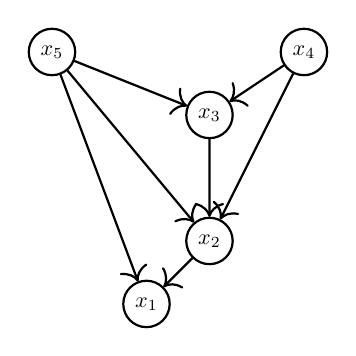
\begin{tikzpicture}[thick,scale=0.8, every node/.style={scale=0.8}]
            \node[circle, draw] at (2, 0)   (x1) {$x_1$};
            \node[circle, draw] at (3, 1)   (x2) {$x_2$};
            \node[circle, draw] at (3, 3)   (x3) {$x_3$};
            \node[circle, draw] at (4.5, 4)   (x4) {$x_4$};
            \node[circle, draw] at (.5, 4)   (x5) {$x_5$};
        
            \draw [-{To[scale=1.5]}, thick] (x5) -- (x3);
            \draw [-{To[scale=1.5]}, thick] (x4) -- (x3);
            \draw [-{To[scale=1.5]}, thick] (x3) -- (x2);
            \draw [-{To[scale=1.5]}, thick] (x5) -- (x2);
            \draw [-{To[scale=1.5]}, thick] (x4) -- (x2);
            \draw [-{To[scale=1.5]}, thick] (x5) -- (x1);
            \draw [-{To[scale=1.5]}, thick] (x2) -- (x1);
        \end{tikzpicture}\\
        (a) & (b)\\
    \end{tabular}
    \caption{(a) denotes the undirected I-map based on the given distribution. (b) denotes the directed I-map by following the dependence in the distribution.}
    \label{fig:imap}
\end{figure}

\subsubsection{Example: construct directed I-map and D-map}

Given the following conditional independence statements
\begin{align*}
    X_1 &\indep X_2 \giv \emptyset \\
    \{ X_1, X_2 \} &\indep X_4 \giv X_3 .
\end{align*}
It is trivial to construct all of the directed D-maps for this set of independence statements. The constructed graphs just need to contain both independence statements. For example, the graph which has no arrows is a valid D-map, as it denotes that every variable is independent of every other variable. Another valid D-map is the DAG in which the independence statements are precisely embedded. Both are seen in figure~\ref{fig:dmap}. Of course, other DAGs are also valid D-maps as long as the given conditional independence statements are part of the DAG, i.e., $\mathcal{L}_P \subseteq \mathcal{L}_G$. 

\begin{figure}[H]
    \centering
    \begin{tabular}{@{}cc@{}}
        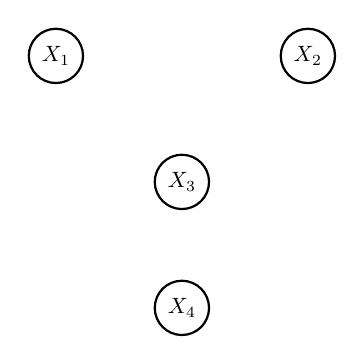
\begin{tikzpicture}[thick,scale=0.8, every node/.style={scale=0.8}]
            \node[circle, draw] at (0, 4)   (x1) {$X_1$};
            \node[circle, draw] at (4, 4)   (x2) {$X_2$};
            \node[circle, draw] at (2, 2)   (x3) {$X_3$};
            \node[circle, draw] at (2, 0)   (x4) {$X_4$};
        \end{tikzpicture}
        &\qquad\qquad\qquad
        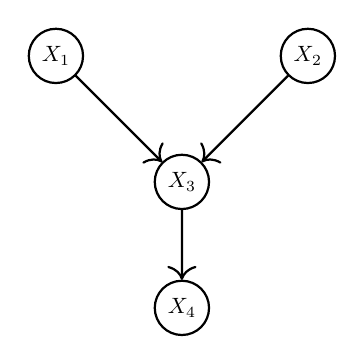
\begin{tikzpicture}[thick,scale=0.8, every node/.style={scale=0.8}]
            \node[circle, draw] at (0, 4)   (x1) {$X_1$};
            \node[circle, draw] at (4, 4)   (x2) {$X_2$};
            \node[circle, draw] at (2, 2)   (x3) {$X_3$};
            \node[circle, draw] at (2, 0)   (x4) {$X_4$};
        
            \draw [-{To[scale=1.5]}, thick] (x1) -- (x3);
            \draw [-{To[scale=1.5]}, thick] (x2) -- (x3);
            \draw [-{To[scale=1.5]}, thick] (x3) -- (x4);
        \end{tikzpicture}\\
        (a) &\qquad\qquad\qquad (b)\\
    \end{tabular}
    \caption{(a) denotes the directed D-map in which all variables are independent of each other, i.e., $G = (V, \emptyset)$. (b) denotes the directed D-map by reconstructing the independences of the given distribution.}
    \label{fig:dmap}
\end{figure}

\noindent To construct I-maps for the conditional independence statements, the most simple I-map is the DAG which contains no independences, i.e., $\mathcal{L}_G = \emptyset$, because the empty set is always a subset of another set ($\mathcal{L}_P$). Then, we can minimize the I-map by removing edges such that the independence statements of the graph are still a subset of the given independence statements. Four possible I-maps are depicted in figure~\ref{fig:imap2}.

\begin{figure}[H]
    \centering
    \begin{tabular}{@{}cc@{}}
        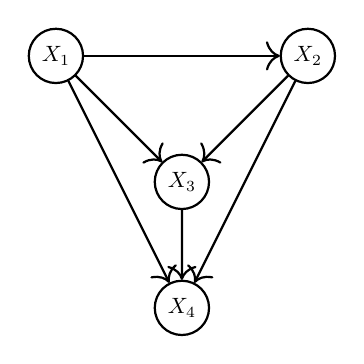
\begin{tikzpicture}[thick,scale=0.8, every node/.style={scale=0.8}]
            \node[circle, draw] at (0, 4)   (x1) {$X_1$};
            \node[circle, draw] at (4, 4)   (x2) {$X_2$};
            \node[circle, draw] at (2, 2)   (x3) {$X_3$};
            \node[circle, draw] at (2, 0)   (x4) {$X_4$};
            
            \draw [-{To[scale=1.5]}, thick] (x1) -- (x3);
            \draw [-{To[scale=1.5]}, thick] (x2) -- (x3);
            \draw [-{To[scale=1.5]}, thick] (x3) -- (x4);
            \draw [-{To[scale=1.5]}, thick] (x1) -- (x2);
            \draw [-{To[scale=1.5]}, thick] (x1) -- (x4);
            \draw [-{To[scale=1.5]}, thick] (x2) -- (x4);
        \end{tikzpicture}
        &\qquad\qquad\qquad
        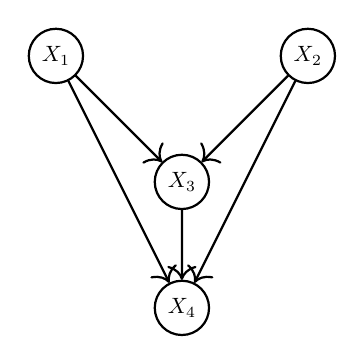
\begin{tikzpicture}[thick,scale=0.8, every node/.style={scale=0.8}]
            \node[circle, draw] at (0, 4)   (x1) {$X_1$};
            \node[circle, draw] at (4, 4)   (x2) {$X_2$};
            \node[circle, draw] at (2, 2)   (x3) {$X_3$};
            \node[circle, draw] at (2, 0)   (x4) {$X_4$};
            
            \draw [-{To[scale=1.5]}, thick] (x1) -- (x3);
            \draw [-{To[scale=1.5]}, thick] (x2) -- (x3);
            \draw [-{To[scale=1.5]}, thick] (x3) -- (x4);
            \draw [-{To[scale=1.5]}, thick] (x1) -- (x4);
            \draw [-{To[scale=1.5]}, thick] (x2) -- (x4);
        \end{tikzpicture}\\
        (a) &\qquad\qquad\qquad (b)\\
        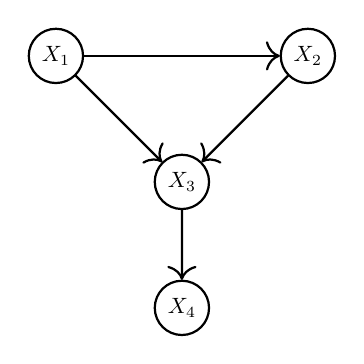
\begin{tikzpicture}[thick,scale=0.8, every node/.style={scale=0.8}]
            \node[circle, draw] at (0, 4)   (x1) {$X_1$};
            \node[circle, draw] at (4, 4)   (x2) {$X_2$};
            \node[circle, draw] at (2, 2)   (x3) {$X_3$};
            \node[circle, draw] at (2, 0)   (x4) {$X_4$};
            
            \draw [-{To[scale=1.5]}, thick] (x1) -- (x3);
            \draw [-{To[scale=1.5]}, thick] (x2) -- (x3);
            \draw [-{To[scale=1.5]}, thick] (x3) -- (x4);
            \draw [-{To[scale=1.5]}, thick] (x1) -- (x2);
        \end{tikzpicture}
        &\qquad\qquad\qquad
        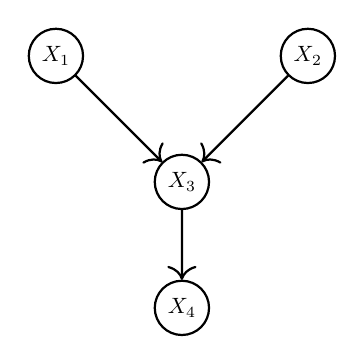
\begin{tikzpicture}[thick,scale=0.8, every node/.style={scale=0.8}]
            \node[circle, draw] at (0, 4)   (x1) {$X_1$};
            \node[circle, draw] at (4, 4)   (x2) {$X_2$};
            \node[circle, draw] at (2, 2)   (x3) {$X_3$};
            \node[circle, draw] at (2, 0)   (x4) {$X_4$};
            
            \draw [-{To[scale=1.5]}, thick] (x1) -- (x3);
            \draw [-{To[scale=1.5]}, thick] (x2) -- (x3);
            \draw [-{To[scale=1.5]}, thick] (x3) -- (x4);
        \end{tikzpicture}\\
        (c) &\qquad\qquad\qquad (d)\\
    \end{tabular}
    \caption{(a) denotes the directed I-map where $\mathcal{L}_G = \emptyset$. (b) denotes the directed I-map where $\mathcal{L}_G = \{X_1 \indep X_2 \giv \emptyset\}$. (c) denotes the directed I-map where $\mathcal{L}_G = \{\{ X_1, X_2 \} \indep X_4 \giv X_3\}$. Finally (d), denotes the directed I-map where $\mathcal{L}_G$ contains both of the conditional independence statements of $\mathcal{L}_P$. Therefore, (d) is also a P-map, because $\mathcal{L}_G \subseteq \mathcal{L}_P$ and $\mathcal{L}_P \subseteq \mathcal{L}_G$, thus $\mathcal{L}_P = \mathcal{L}_G$. }
    \label{fig:imap2}
\end{figure}

\newpage
\section{Causality}

The concept of \textbf{causality} is often misinterpreted due to statistical associations in the data that lead to the belief that the data has causal properties. The phrase "\textit{correlation does not imply causation}" is widely used to point out that it is not possible to deduce a cause-effect relationship from an association. Nevertheless, causality is often used in place of association. For example, when two events happen one after another in a temporal way, it is often assumed that the first event caused the second event.

More specifically, for a distribution $p(a, b)$, we could write it as either $p(a \giv b)p(b)$ or $p(b \giv a)p(a)$. In the former, we might think that $b$ caused $a$, and in the latter, we might think that $a$ caused $b$. This is not very meaningful, as they both represent the same distribution. Bayesian networks, formally, only make independence statements, not causal statements. Nonetheless, in constructing BNs, it can be helpful to think about dependencies in terms of causation since our intuitive understanding is usually framed in how one variable \textbf{influences} another.   

\subsection{Simpson's paradox}

Simpson's paradox is a phenomenon in which a trend appears in several groups of data but disappears or reverses when the groups are aggregated. 

Sprenger and Weinberger~\cite{paradox-simpson} provide an example of the paradox. Consider a medical trial in which two groups, men and women, are tested on the effect of some treatment $T$. The treatment can either result in a success or a failure denoted by the random variable $S = \{0, 1\}$. Table~\ref{tab:treat} summarizes the effect on the overall population ($N=52$), and separately for men and women. 

\begin{table}[H]
    \centering
    \caption{Simpson's paradox in which the association at the population level (positive, negative, independent) changes at the level of subpopulations.}\label{tab:treat}
    \vspace{5mm}
    \makebox[\linewidth]{
        \begin{tabular}{c|ccc|ccc|ccc}
            \toprule
                \multicolumn{1}{c}{} & \multicolumn{3}{c}{\textbf{Full population, $N=52$}} & \multicolumn{3}{c}{\textbf{Men ($M$), $N=20$}} & \multicolumn{3}{c}{\textbf{Women ($\neg M$), $N=32$}} \\ \hline
            % \cmidrule(rl){2-4} \cmidrule(rl){6-8} \cmidrule(rl){10-12} 
                & \emph{Success} & \emph{Failure} & \emph{Success} & \emph{Success} & \emph{Failure} & \emph{Success} & \emph{Success} & \emph{Failure} & \emph{Success}\\
                & ($S$) & ($\neg S$) & \emph{Rate} & & & \emph{Rate} & & & \emph{Rate} \\
            \midrule
                \textbf{Treatment} & 20 & 20 & 50\% & 8 & 5 & $\approx 61\%$ & 12 & 15 & $\approx 44\%$ \\
                ($T$) &&&&&&&&\\
                \textbf{Control} & 6 & 6 & 50\% & 4 & 3 & $\approx 57\%$ & 2 & 3 & $\approx 40\%$ \\
                ($\neg T$) &&&&&&&&\\
            \bottomrule
        \end{tabular}
    }
\end{table}

\noindent We see from the table that the treatment yields ineffective results at the population level, success rate being 50\% for both treatment and control, however it leads to higher success rates than control for the group of men and the group of women. 

In the form of conditional probabilities, we see that
$$
    p(S \giv T) = p(S \giv \neg T)
$$
while at the same time the inequalities also hold
\begin{align*}
    p(S \giv T, M) &> p(S \giv \neg T, M) \\
    p(S \giv T, \neg M) &> p(S \giv \neg T, \neg M)
\end{align*}
\noindent Assuming that we know the gender of the patient, then from the results in table~\ref{tab:treat}, we would use the treatment, as it has a higher success rate for both the female sample as well as the male sample. However, assuming that we do \textit{not} know the gender, the results imply that there is no effect by using the treatment, although we know that the patient is either male or female. 

To explain the paradox, consider the success rates for both men and women. We see a positive association between treated men and treated women compared to their untreated counterparts. More specifically, 61\% vs 57\% for the men group and 44\% vs 40\% for the women group. There are two key observations here to understand why the positive association vanishes in the aggregate. (1) first, notice how the success rate is still higher for \textit{untreated men} than for \textit{treated women} (57\% vs 44\%). This suggests that not only the treatment but also the gender is a relevant variable for the success rate. (2) second, the treatment group in total is majority female, i.e., 27 women vs 13 men, whereas the control group is majority male, i.e., 5 women vs 7 men. In summary, there is a lack of population-level correlation between treatment and success results, because men are more likely to recover from the treatment than women, and men are less likely to be in the treatment group.

When computing the conditional probabilities for the success rates given the treatment and subpopulations, i.e., men and women, we see where the 50\% is derived from.
\begin{align*}
    p(S \giv T) &= \sum_M p(S \giv T, M) p(M \giv T) \\
    &= p(S \giv T, M) p(M \giv T) + p(S \giv T, \neg M) p(\neg M \giv T) \\
    &= \frac{8}{13} \times \frac{13}{40} + \frac{12}{27} \times \frac{27}{40} \\ 
    &= \frac{8}{40} + \frac{12}{40} = \frac{20}{40} = 0.5\\[2em]
    p(S \giv \neg T) &= \sum_M p(S \giv \neg T, M) p(M \giv \neg T) \\
    &= p(S \giv \neg T, M) p(M \giv \neg T) + p(S \giv \neg T, \neg M) p(\neg M \giv \neg T) \\
    &= \frac{4}{7} \times \frac{7}{12} + \frac{2}{5} \times \frac{5}{12}\\
    &= \frac{4}{12} + \frac{2}{12} = \frac{6}{12} = 0.5
\end{align*}

\noindent To motivate the concept of causality using Simpson's paradox, recall that the success rate for untreated men is higher than the success rate of treated women, i.e., $p(S \giv \neg T, M) > p(S \giv T, \neg M)$. The implication here is that we assumed that treatment is the cause of success, as denoted in the simple DAG in figure~\ref{fig:simp}a. However, clearly gender plays a role in this association. We see that men are less likely to be in the treatment group, which means that gender has an effect on the treatment variable. We also see that men are more likely to recover, which means that gender has an effect on the success rate. Therefore, there is a \textit{common cause} gender that influences both treatment and success, as denoted in figure~\ref{fig:simp}b. 

\begin{figure}[H]
    \centering
    \begin{tabular}{@{}cc@{}}
        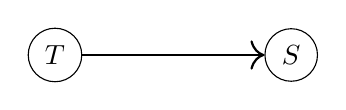
\begin{tikzpicture}
            \node[circle, draw] at (0, 0)   (T) {$T$};
            \node[circle, draw] at (3, 0)   (S) {$S$};
            \draw [-{To[scale=1.5]}, thick] (T) -- (S);
        \end{tikzpicture}
        &
        \begin{tikzpicture}
            \node[circle, draw] at (0, 0)   (T) {$T$};
            \node[circle, draw] at (3, 0)   (S) {$S$};
            \node[circle, draw, fill=purple!20] at (0, 2)   (G) {$M$};
            \draw [-{To[scale=1.5]}, thick] (T) -- (S);
            \draw [-{To[scale=1.5]}, thick, dashed] (G) -- (T);
            \draw [-{To[scale=1.5]}, thick, dashed] (G) -- (S);
        \end{tikzpicture}\\
        (a) & (b)\\
    \end{tabular}
    \caption{(a) the relationship between treatment $T$ and success $S$ prior to knowing that the common cause gender $M$ might affect both treatment and success. (b) now with the inclusion of gender as the common cause of treatment and success.}
    \label{fig:simp}
\end{figure}

\subsection{Causal Bayesian Networks}

As shown in Simpson's paradox, it is impossible to define causality in terms of probabilities alone. Instead, causality can be modeled by conveying additional information beyond independence information. \textbf{Causal Bayesian networks} are Bayesian networks where the edges between the nodes convey information beyond the independence structure of normal Bayesian networks. 

In figure~\ref{fig:simp}b, we see a model for the treatment-success problem in which we identified gender to be a common cause for both the treatment and success. The joint distribution for this model looks like 
$$
    p(S, T, M) = p(S \giv T, M) p(T \giv M) p(M) .
$$
In causal interpretation, if we \textit{intervene} and use the treatment, then the term $p(T \giv M)$ should have no role in the experiment. We 'forcefully' intervene and set $T$ to be true. We use the idea of an \textbf{atomic intervention}, in which a single variable is set in a particular state. 

To intervene in causal inference, Judea Pearl constructed the \textbf{do-calculus}, which contrasts an observational ('see') inference $p(x \giv y)$ with a causal ('make' or 'do') inference $p(x \giv \text{do}(y))$. The do-operator is defined as follows.
\\
\begin{theorem}
    \textbf{Pearl's do-operator.} Inferring the effect of setting variables $X_{c_1}, \dots, X_{c_k}, c_k \in C$, in states $x_{c_1}, \dots, x_{c_k}$, is equivalent to standard evidential inference in the \textit{post intervention distribution}:
    \begin{align*}
        p(X \giv \text{do}(X_{c_1} = x_{c_1}), \dots, \text{do}(X_{c_k} = x_{c_k})) &= \frac{p(X_1, \dots, X_n \giv x_{c_1}, \dots, x_{c_k})}{\prod_{i=1}^K p(X_{c_i} \giv \text{pa}(X_{c_i}))} \\[1em]
        &= \prod_{j \notin C} p(X_j \giv \text{pa}(X_j))
    \end{align*}
    where any parental states $\text{pa}(X_j)$ of $X_j$ are set in their evidential states. An alternative notation to the do-operator is $p(X \giv \giv x_{x_1}, \dots, x_{x_k})$. 
\end{theorem}

\noindent The definition implies that for those variables for which we intervene and set in a particular state, the corresponding terms $p(X_j \giv \text{pa}(X_j))$ are removed from the original Bayesian network. 

Considering the treatment-success example, we intervene and set treatment to true, for which we can compute the probability of success given that we forced treatment, i.e., 
\begin{align*}
    p(S \giv \text{do}(T)) &= \sum_M p(S \giv T, M) p(M) \\
    &= \frac{8}{13} \times \frac{20}{52} + \frac{12}{27} \times \frac{32}{52} \approx 0.5102\\
    p(S \giv \text{do}(\neg T)) &= \sum_M p(S \giv \neg T, M) p(M) \\
    &= \frac{4}{7} \times \frac{20}{52} + \frac{2}{5} \times \frac{32}{52} \approx 0.4659
\end{align*}
\noindent Using the do-operator, we see that the treatment is effective at the population-level ($51.02\%$ vs $46.59\%$), whereas before the treatment was ineffective (50\% vs 50\%). In general, if the treatment is effective in every subpopulation, it should also be effective in the total population.
\\\\
\noindent For a Bayesian network to have a \textbf{causal interpretation}, the ancestral order of the random variables must correspond to the temporal order. In other words, the variables which have no parents must be the first in the temporal ordering. 

\subsection{Structural Causal Models}

To deal rigorously with questions of causality, we need a formal specification to describe assumptions pertaining to the causal story behind the dataset. The concept of the \textbf{structural causal model} (SCM) intends to describe the relevant features of the world and how they interact with each other. Such a model describes how nature assigns values to variables of interest. 
\\
\begin{theorem}
    \textbf{Structural Causal Models.} A structural causal model consists of two sets $U$ and $V$, and a set of functions $f$ that assigns each variable in $V$ a value based on the values of the other variables in the model. 
    \\\\
    A variable $X$ is a \textit{direct cause} of a variable $Y$ if $X$ appears in the function that assigns $Y$'s value, i.e., $f_Y(X)$. 
    \\\\
    \noindent The variables in $U$ are called \textit{exogenous variables} (or noise variables, or disturbance variables), and cannot be descendants of any other variables, i.e., they are the root nodes in the graph. The variables in $V$ are called \textit{endogenous variables}, which means that they are descendants of at least one exogenous variable.   
\end{theorem}

\noindent Every SCM is associated with a graphical causal model, sometimes called an \textbf{augmented functional graph}. Analytically, SCMs may be represented by a DAG. For instance, the DAG consisting of $X \rightarrow Y$, in a causal context, has the meaning of variable $X$ being exogenous (root) and the cause of variable $Y$. In other words, the function that assigns $Y$'s value depends on the value of variable $X$. 

As an example, consider the following setup. The sex of a person is a cause for the person's height, and the height is a cause for the performance in playing basketball. 
\begin{align*}
    V = &\{\text{Height, Sex, Performance}\}, \qquad U = \{U_1, U_2, U_3\}, \qquad F = \{f_1, f_2\}\\
    &\text{Sex} = U_1\\
    &\text{Height} = f_1(\text{Sex}, U_2)\\
    &\text{Performance} = f_2(\text{Height}, \text{Sex}, U_3)
\end{align*}

\noindent Here, the exogenous variables in $U$ represent unmeasured or unknown factors that affect the variables in $V$. These factors are sometimes called \textbf{error terms} or \textbf{omitted factors}. Figure~\ref{fig:scm} denotes the graphical model corresponding to this SCM. 

\begin{figure}[H]
    \centering
    \begin{tikzpicture}
        \node[circle, draw] at (2, 4)   (u1) {$U_1$};
        \node[circle, draw] at (5, 2)   (u2) {$U_2$};
        \node[circle, draw] at (.5, 1)   (u3) {$U_3$};
        \node[circle, draw] at (2, 2)   (s) {$S$};
        \node[circle, draw] at (3.5, 1)   (h) {$H$};
        \node[circle, draw] at (2, 0)   (p) {$P$};
        
        \draw [-{To[scale=1.5]}, thick] (u1) -- (s);
        \draw [-{To[scale=1.5]}, thick] (s) -- (p);
        \draw [-{To[scale=1.5]}, thick] (s) -- (h);
        \draw [-{To[scale=1.5]}, thick] (u2) -- (h);
        \draw [-{To[scale=1.5]}, thick] (h) -- (p);
        \draw [-{To[scale=1.5]}, thick] (u3) -- (p);
    \end{tikzpicture}
    \caption{A directed acyclic graph corresponding to the causal sex-height-performance SCM example.}
    \label{fig:scm}
\end{figure}

\noindent SCMs have the advantage of being more generic compared to causal Bayesian networks, i.e., every causal Bayesian network can be represented by an SCM, but not the other way around. For example, SCMs may be cyclic, i.e., the function on two variables depend on each other, which implies that the graph is also cyclic. Cyclic graphs significantly increase complexity in terms of joint probability distributions. 

\subsection{Intervention}

The ultimate aim of statistics is to predict the \textbf{effects of interventions}. During the collection of data on wildfires, we are looking for something we can intervene upon in order to decrease wildfire frequency. A mere association between two variables does not necessarily or even usually imply that one of those variables causes the other. For instance, an increase in ice cream sales is correlated with an increase in violent crimes, not because ice cream causes crime, but because both ice cream sales and violent crime are more common in hot weather. Hot weather is a common cause that might be unknown when looking at purely observational data. 

For this reason, the \textbf{randomized controlled experiment} is considered a golden standard in statistics. In such experiments, all factors that may influence the outcome are either \textit{static} or \textit{vary at random}, except for one. That is, the factor that we \textit{control} for, so that any changes in the outcome variable must be due to the control variable. Unfortunately, many experiments are neither random nor able to be properly controlled. We cannot control the weather, so we cannot randomize the prominent variables that affect wildfires. 

In cases where randomized controlled experiments are not practical, researchers instead perform \textbf{observational studies}, in which they merely record data, rather than controlling for certain variables. The problem of observational data is that it is difficult to untangle the \textbf{causal} from the \textbf{correlative}. 

As we saw in the Simpson's paradox example, a common cause for both the treatment and the success rate is the gender of the participant. If we intervene on the gender variable, it would lead to the causal effect of the treatment on the success rate. 

The difference between \textbf{intervening} on a variable and \textbf{conditioning} on that variable is that an intervention \textbf{changes} the underlying system, whereas conditioning merely narrows the space of cases. When we intervene on a variable in a model, we fix its value, by which the system is changed, and the values of other variables often change as well. When we condition on a variable, we change nothing. However, what does change in a conditioning is the perception of the world, not the world itself. 

\begin{figure}[H]
    \centering
    \begin{tabular}{@{}ccc@{}}
        \begin{tikzpicture}
            \node[circle, draw, minimum size=.8cm] at (0, 0)   (I) {$I$};
            \node[circle, draw, minimum size=.8cm] at (4, 0)   (V) {$V$};
            \node[circle, draw, minimum size=.8cm] at (2, 2)   (W) {$W$};
            \node[circle, draw, minimum size=.8cm] at (0, 2)   (UI) {$U_I$};
            \node[circle, draw, minimum size=.8cm] at (4, 2)   (UV) {$U_V$};
            \node[circle, draw, minimum size=.8cm] at (2, 4)   (UW) {$U_W$};
            
            \draw [-{To[scale=1.5]}, thick] (UI) -- (I);
            \draw [-{To[scale=1.5]}, thick] (UV) -- (V);
            \draw [-{To[scale=1.5]}, thick] (UW) -- (W);
            \draw [-{To[scale=1.5]}, thick] (W) -- (I);
            \draw [-{To[scale=1.5]}, thick] (W) -- (V);
        \end{tikzpicture}
        & \qquad\qquad\qquad &
        \begin{tikzpicture}
            \node[circle, draw, minimum size=.8cm] at (0, 0)   (I) {$I$};
            \node[circle, draw, minimum size=.8cm] at (4, 0)   (V) {$V$};
            \node[circle, draw, minimum size=.8cm] at (2, 2)   (W) {$W$};
            \node[circle, draw, minimum size=.8cm] at (4, 2)   (UV) {$U_V$};
            \node[circle, draw, minimum size=.8cm] at (2, 4)   (UW) {$U_W$};
            
            \draw [-{To[scale=1.5]}, thick] (UV) -- (V);
            \draw [-{To[scale=1.5]}, thick] (UW) -- (W);
            \draw [-{To[scale=1.5]}, thick] (W) -- (V);
        \end{tikzpicture}\\
        (a) & & (b)\\
    \end{tabular}
    \caption{(a) graphical causal model of the temperature $W$ as the common cause for increased ice cream sales $I$ and increased violent crimes $V$. (b) the causal graph of (a), in which we intervene on $I$ by setting its value, and changing the structure of the model.}
    \label{fig:inter}
\end{figure}

\noindent Figure~\ref{fig:inter}a illustrates the graphical model corresponding to the ice cream example. We see that $W$ is the common cause for both $I$ and $V$. The $U_i$ variables are the exogenous variables that add a noise factor to the distribution. Notice that by intervening on the increase of ice cream sales $I$, denoted in figure~\ref{fig:inter}b, we surgically remove all edges directed into the variable. As a result, violent crimes are uncorrelated with ice cream sales, since we fixed the value of ice cream sales by which the association with temperature vanishes. 

In terms of probability terminology, $p(Y=y \giv X=x)$ represents the population distribution of $Y$ among individuals whose $X$ value is $x$, i.e., filtering a table of data based on the value of $X$. On the other hand, $p(Y=y \giv \text{do}(X=x))$ represents the population distribution of $Y$ if \textit{everyone in the population} had their $X$ value fixed at $x$. 

It is worth noting that we make the assumption that the \textbf{intervention has no side-effects}. That is, assigning the value $x$ for the variable $X$ for an individual does not alter subsequent variables in a direct way. For example, being given a certain drug at random might have a different effect on recovery than being forced to take a drug against one's religious objections. In the presence of side-effects, they need to be explicitly specified in the model.

\subsection{The Adjustment Formula}

In the aforementioned treatment-success example, we used the do-operator to intervene and set the treatment variable $T$, and subsequently observed the distribution of the success rate $S$. To find out how effective the treatment is in the population, we imagine a  hypothetical intervention by which we administer the treatment uniformly to the entire population $p(S \giv \text{do}(T))$, and compare the success rate to what would happen if we prevent everyone from getting the treatment $p(S \giv \text{do}(\neg T))$. This is known as the \textbf{causal effect difference} or \textbf{average causal effect}~(ACE). Thus, we can estimate the ACE with 
\begin{align*}
    ACE &= p(S \giv \text{do}(T)) - p(S \giv \text{do}(\neg T)) \\[1em]
    &= \sum_M p(S \giv T, M) p(M) - \sum_M p(S \giv \neg T, M) p(M) \\[1em]
    &= 0.5102 - 0.4659 \approx 0.0443 .
\end{align*}

\noindent A more informal interpretation of $ACE$ is that it is simply the difference in the fraction of the population that would recover successfully if everyone was given the treatment compared to when no one was given the treatment. 
\\
\begin{theorem}
    \textbf{Adjustment formula.} Given a causal graphical model with variables $X$ and $Z$ being the causes of variable $Y$, and additionally $Z$ being the cause of $X$. The joint probability distribution is then 
    $$
        p(Y \giv X, Z)p(X \giv Z)p(Z) .
    $$
    \begin{center}
        \begin{tikzpicture}
            \node[circle, draw, minimum size=.8cm] at (0, 0)   (X) {$X$};
            \node[circle, draw, minimum size=.8cm] at (2, 0)   (Y) {$Y$};
            \node[circle, draw, minimum size=.8cm] at (1, 1.5)   (Z) {$Z$};
            
            \draw [-{To[scale=1.5]}, thick] (Z) -- (Y);
            \draw [-{To[scale=1.5]}, thick] (Z) -- (X);
            \draw [-{To[scale=1.5]}, thick] (X) -- (Y);
        \end{tikzpicture}
    \end{center}
    Intervening on $X$ removes the causal relation between $X$ and $Z$. The equation for the \textbf{adjustment formula} is then
    $$
        p(Y = y \giv \text{do}(X = x)) = \sum_z p(Y=y \giv X=x, Z=z)p(Z=z)
    $$
    and computes the association between $X$ and $Y$ for each value $z$ of $Z$, then averages over those values. This procedure is referred to as "adjusting for $Z$" or "controlling for $Z$". The more general formula is
    $$
        p(Y = y \giv \text{do}(X = x)) = \sum_z p(Y=y \giv X=x, \text{pa}(X)=z)p(\text{pa}(X)=z)
    $$
    where we sum over each $z$, that is, each value of pa($X$). 
\end{theorem}

\noindent Graphically, the structural causal model~(SCM) corresponding to the treatment-success model is seen in figure~\ref{fig:adj}a. The effect of intervention on the structure of the model is seen in figure~\ref{fig:adj}b. Note that in a \textbf{randomized controlled experiment}, no adjustment is needed, since in such a setting the data are generated by a model which already possesses the structure of figure~\ref{fig:adj}b. 

\begin{figure}[H]
    \centering
    \begin{tabular}{@{}ccc@{}}
        \begin{tikzpicture}
            \node[circle, draw, minimum size=.8cm] at (0, 0)   (T) {$T$};
            \node[circle, draw, minimum size=.8cm] at (4, 0)   (S) {$S$};
            \node[circle, draw, minimum size=.8cm] at (2, 2)   (M) {$M$};
            \node[circle, draw, minimum size=.8cm] at (0, 2)   (UT) {$U_T$};
            \node[circle, draw, minimum size=.8cm] at (4, 2)   (US) {$U_S$};
            \node[circle, draw, minimum size=.8cm] at (2, 4)   (UM) {$U_M$};
            
            \draw [-{To[scale=1.5]}, thick] (UT) -- (T);
            \draw [-{To[scale=1.5]}, thick] (US) -- (S);
            \draw [-{To[scale=1.5]}, thick] (UM) -- (M);
            \draw [-{To[scale=1.5]}, thick] (M) -- (T);
            \draw [-{To[scale=1.5]}, thick] (M) -- (S);
            \draw [-{To[scale=1.5]}, thick] (T) -- (S);
        \end{tikzpicture}
        & \qquad\qquad\qquad &
        \begin{tikzpicture}
            \node[circle, draw, minimum size=.8cm] at (0, 0)   (T) {$T$};
            \node[circle, draw, minimum size=.8cm] at (4, 0)   (S) {$S$};
            \node[circle, draw, minimum size=.8cm] at (2, 2)   (M) {$M$};
            \node[circle, draw, minimum size=.8cm] at (4, 2)   (US) {$U_S$};
            \node[circle, draw, minimum size=.8cm] at (2, 4)   (UM) {$U_M$};
            
            \draw [-{To[scale=1.5]}, thick] (US) -- (S);
            \draw [-{To[scale=1.5]}, thick] (UM) -- (M);
            \draw [-{To[scale=1.5]}, thick] (M) -- (S);
            \draw [-{To[scale=1.5]}, thick] (T) -- (S);
        \end{tikzpicture}\\
        (a) & & (b)\\
    \end{tabular}
    \caption{(a) SCM of treatment-success example. (b) SCM of treatment-success example, in which we intervened on $T$. }
    \label{fig:adj}
\end{figure}

\subsection{The Backdoor Criterion}

In trying to determine the effect of a variable $X$ on another $Y$, we should adjust for the parents of $X$. But what if the variable $X$ has \textit{unmeasured parents}, that may be inaccessible for measurement? In those cases, we need to find an alternative set of variables to adjust for. 

The central question becomes: Under what conditions does a causal story permit us to compute the causal effect of one variable on another, from data obtained by passive observations, with no interventions? Because we represent \textit{causal stories} with graphs, the question becomes a graph-theoretical problem: Under what conditions is the structure of the causal graph \textit{sufficient} for computing a causal effect from a given dataset? 

One of the most important tools to determine whether we can compute a causal effect is a simple test called the \textbf{backdoor criterion}. The backdoor criterion allows us to determine, for any two variables $X$ and $Y$ in a causal model represented by a DAG, which set of variables $Z$ in that model should be conditioned on when searching for the causal relationship between $X$ and $Y$. 
\\
\begin{theorem}
    \textbf{Backdoor Criterion.} Given an ordered pair of variables ($X, Y$) in a directed acyclic graph $G$, a set of variables $Z$ satisfies the backdoor criterion relative to $(X, Y)$
    \begin{enumerate}
        \item if $X, Y \not \in Z$; and
        \item if no node in $Z$ is a descendant of $X$; and
        \item if $Z$ blocks every path between $X$ and $Y$ that contains an arrow into $X$. 
    \end{enumerate}
\end{theorem}

\noindent If a set of variables $Z$ satisfies the backdoor criterion for $X$ and $Y$, then the causal effect of $X$ on $Y$ is given by the formula
$$
    p(Y = y \giv \text{do}(X=x)) = \sum_z p(Y=y \giv X=x, Z=z)p(Z=z)
$$
just like when we adjust for the parents of $X$, pa($X$). Note that pa($X$) always satisfies the backdoor criterion. For the backdoor criterion, we like to condition on a set of nodes $Z$ such that 
\begin{enumerate}
    \item All \textit{spurious paths} from $X$ to $Y$ are blocked. Spurious relationships refers to two variables that appear to be causal, but in reality are not causal, due to a common cause (confounder). 
    \item All directed paths from $X$ to $Y$ are unblocked. 
    \item No new spurious paths are created. 
\end{enumerate}

\noindent When trying to find the \textbf{causal effect} of $X$ on $Y$, we want the nodes we condition on to block any ``backdoor'' path, in which one end has an arrow into $X$. Such paths may make $X$ and $Y$ dependent, even though they are not transmitting any causal influence from $X$. If we do not block them, they will confound the effect that $X$ has on $Y$. The first condition~(1) is hereby met. Furthermore, we do not want to condition on any descendants of $X$, because these nodes would be affected by an intervention on $X$, and might themselves affect $Y$, i.e., conditioning on them would block these pathways. The second condition~(2) is also met. Finally, we should refrain from conditioning on any collider that would unblock a new path between $X$ and $Y$. The third condition~(3) is therefore also met. 

As an example, consider the following causal graph shown in figure~\ref{fig:causal}, in which we are trying to measure the effect of a new drug ($X$) on recovery ($Y$). We also measure some weight ($W$), which has an effect on recovery. Furthermore, we know that socioeconomic status ($Z$) affects both weight and the choice to receive treatment. In this study, however, we did not record the socioeconomic status. 

\begin{figure}[H]
    \centering
    
    \begin{tikzpicture}
        \node[circle, draw] at (0, 0)   (X) {$X$};
        \node[circle, draw] at (3, 0)   (Y) {$Y$};
        \node[circle, draw] at (3, 2)   (W) {$W$};
        \node[circle, draw] at (0, 2.3)   (Z) {$Z$};
        \draw [-{To[scale=1.5]}, thick] (X) -- (Y);
        \draw [-{To[scale=1.5]}, thick] (W) -- (Y);
        \draw [-{To[scale=1.5]}, thick, dashed] (Z) -- (X);
        \draw [-{To[scale=1.5]}, thick, dashed] (Z) -- (W);
    \end{tikzpicture}
    \caption{Causal graph in which $Z$ is unobserved, but is a causal factor of both $X$ and $W$. }
    \label{fig:causal}
\end{figure}

\noindent Since $Z$ is not observed (as indicated by the dashed line), we search for an \textit{observed variable} that meets the backdoor criterion from $X$ to $Y$. We see that $W$ also meets the backdoor criterion, because $W$ blocks the path $X \leftarrow Z \rightarrow W \rightarrow Y$. Therefore, adjusting for $W$ will give us the causal effect of $X$ on $Y$. Using the adjustment formula, we find
$$
    p(Y=y \giv \text{do}(X=x)) = \sum_w p(Y=y \giv X=x, W=x)p(W=w)
$$
\noindent As long as $W$ is observed, we can estimate this sum from the observational data. 

\subsubsection{Example: Compliance to backdoor criterion}

Consider the causal graph in figure~\ref{fig:bdex}. Which sets of variables fit the backdoor criterion given that we want to know the causal effect of a pair of variables. 

\begin{figure}[H]
    \centering
    
    \begin{tikzpicture}
        \node[circle, draw] at (0, 3)   (A) {$A$};
        \node[circle, draw] at (1, 2)   (B) {$B$};
        \node[circle, draw] at (2, 3)   (C) {$C$};
        \node[circle, draw] at (3, 2)   (D) {$D$};
        \node[circle, draw] at (2, 1)   (E) {$E$};
        \node[circle, draw] at (2, -.3)   (F) {$F$};
        
        \draw [-{To[scale=1.5]}, thick] (A) -- (B);
        \draw [-{To[scale=1.5]}, thick] (C) -- (B);
        \draw [-{To[scale=1.5]}, thick] (B) -- (E);
        \draw [-{To[scale=1.5]}, thick] (C) -- (D);
        \draw [-{To[scale=1.5]}, thick] (D) -- (E);
        \draw [-{To[scale=1.5]}, thick] (E) -- (F);
    \end{tikzpicture}
    \caption{Example causal DAG.}
    \label{fig:bdex}
\end{figure}

\noindent Which set of variables satisfy the backdoor criterion given we want to measure the
\begin{itemize}
    \item \textbf{Causal effect of $B$ on $E$?} There are 2 nodes that have an arrow into $B$, i.e., $A$ and $C$. Only $C$ lies on a path between $B$ and $E$. Therefore, conditioning on any combination of variables between $B$ and $E$ meets the backdoor criterion. 
    $$
        \{ \{C\}, \{D\}, \{C, D\}, \{A, C\}, \{A, D\}, \{A, C, D\}\}
    $$
    \item \textbf{Causal effect of $B$ on $F$?} The same two nodes as in the previous question have an arrow into $B$. Thus, the variables on the path containing $C$ satisfy the backdoor criterion. These are the exact same as the previous question. 
    $$
        \{ \{C\}, \{D\}, \{C, D\}, \{A, C\}, \{A, D\}, \{A, C, D\}\}
    $$
    \item \textbf{Causal effect of $A$ on $F$?} In this case, notice that there are no arrows which lead into $A$. This means that we can condition on the empty set, as well as all variables, and their combinations, which do not lie on the directed paths between $A$ and $F$. 
    $$
        \{ \emptyset, \{C\}, \{D\}, \{C, D\}\}
    $$
\end{itemize}

\subsubsection{Example: adjusting for collider}

Adjusting for colliders should be refrained from, as colliders, when conditioned upon, may unblock a path. However, in some instances, it is unavoidable to avoid conditioning on colliders, as can be seen in figure~\ref{fig:bdex2}. 

\begin{figure}[H]
    \centering
    
    \begin{tikzpicture}
        \node[circle, draw] at (0, 0)   (X) {$X$};
        \node[circle, draw] at (2, 0)   (Y) {$Y$};
        \node[circle, draw] at (-2, 3)   (E) {$E$};
        \node[circle, draw] at (1, 2)   (Z) {$Z$};
        \node[circle, draw] at (4, 3)   (A) {$A$};
        
        \draw [-{To[scale=1.5]}, thick] (X) -- (Y);
        \draw [-{To[scale=1.5]}, thick] (E) -- (X);
        \draw [-{To[scale=1.5]}, thick] (Z) -- (X);
        \draw [-{To[scale=1.5]}, thick] (Z) -- (Y);
        \draw [-{To[scale=1.5]}, thick] (E) -- (Z);
        \draw [-{To[scale=1.5]}, thick] (A) -- (Z);
        \draw [-{To[scale=1.5]}, thick] (A) -- (Y);
    \end{tikzpicture}
    \caption{Example causal DAG, in which there is an unavoidable collider when deriving the nodes that satisfy the backdoor criterion.}
    \label{fig:bdex2}
\end{figure}

\noindent Here, there are 4 backdoor paths from $X$ to $Y$, which all traverse $Z$ at some point. $Z$ is a collider in $E \rightarrow Z \leftarrow A$. The possible paths are:
\begin{itemize}
    \item[] $X \leftarrow E \rightarrow Z \rightarrow Y$
    \item[] $X \leftarrow E \rightarrow Z \leftarrow A \rightarrow Y$
    \item[] $X \leftarrow Z \rightarrow Y$
    \item[] $X \leftarrow Z \leftarrow A \rightarrow Y$
\end{itemize}
\noindent Naively conditioning on $Z$ will unblock (activate) the path $X \leftarrow E \rightarrow Z \leftarrow A \rightarrow Y$, because of the collider which violates the backdoor criterion. Therefore, to block all backdoor paths, we need to condition on one of the following sets of variables: $\{E, Z\}, \{Z, A\}, \{E, Z, A\}$. 

\subsection{Counterfactuals}

Counterfactuals allow us to answer questions about what would have happened had we done something differently. This type of reasoning revolves around retrospective reasoning. Counterfactual reasoning uses both the semantics of associational reasoning and interventional reasoning. 

\noindent To resolve a counterfactual query, we need to incorporate two aspects:
\begin{enumerate}
    \item An observational aspect; and
    \item An evaluation of a variable after an intervention.
\end{enumerate}
\noindent As an example, suppose there exists an effective treatment for an eye disease. The treatment works for 99\% of all patients, and the patients are cured ($B=0$). If untreated, these patients turn blind within a day ($B=1$). For the remaining 1\%, the treatment has the opposite effect, as they turn blind within a day ($B=1$). If they were untreated, they would have regained normal vision ($B=0$). In other words
\begin{align*}
    p(B=0 \giv T=1) = 0.99 \qquad p(B=0 \giv T=0) = 0.01
\end{align*}
\noindent Furthermore, suppose which category a patient belongs to is controlled by a rare condition ($R$) that is unknown to the doctor. The doctor's decision to administer the treatment is thus independent of this condition, i.e., $R \indep T$. The causal graph from this problem is trivial, $T \rightarrow B$. Note that we do not include $R$, because it is an unobserved variable. 

Now suppose we observe a patient that came to the hospital with poor eyesight, received the treatment, and went blind, i.e., $P(B=1 \giv T=1)$. A relevant counterfactual question is
\begin{center}
    \textit{What would have happened if the doctor had not administered the treatment?}
\end{center}
\noindent Here, the observational aspect is that the patient went blind after receiving the treatment. We want to evaluate the probability of going blind ($B$) after intervening and \textbf{not} giving the treatment to the patient (do$(T=0)$). This seems impossible due to conditioning on $B$ and $T$, and at the same time, we are interested in the relationship between $B$ and $T$. 

\subsubsection{Twin network}

In a causal Bayesian network, we can construct a \textbf{twin network} to answer counterfactual questions. The idea is to consider 2 versions of the random variables. In the actual world where we made the prior observation, we have $B$ and $T$. In the \textit{counterfactual world}, we have their mirror counterparts $B^*$ and $T^*$. 

Prior to constructing the twin network, we need to turn the causal graph into an SCM by introducing noise variables. The unobserved rare condition $R$ might be modelled as a noise variable. Additionally, the decision of whether to administer the treatment or not might be influenced by some noise $N_T$, e.g., the majority of the doctor's patients turned blind yesterday, thus causing him to be more careful. The following equations denote the causal dependencies of the SCM, and figure~\ref{fig:cfex} illustrates the causal graph.
\begin{align*}
    T &= f_T(N_T)\\
    B &= f_B(T, R)
\end{align*}

\begin{figure}[H]
    \centering
    
    \begin{tikzpicture}
        \node[circle, draw] at (0, 0)   (T) {$T$};
        \node[circle, draw] at (2, 0)   (B) {$B$};
        \node[circle, draw] at (0, 2)   (NT) {$N_T$};
        \node[circle, draw] at (2, 2)   (R) {$R$};
        
        \draw [-{To[scale=1.5]}, thick] (T) -- (B);
        \draw [-{To[scale=1.5]}, thick] (NT) -- (T);
        \draw [-{To[scale=1.5]}, thick] (R) -- (B);
    \end{tikzpicture}
    \caption{Causal graph for example counterfactual problem.}
    \label{fig:cfex}
\end{figure}

\noindent Furthermore, we know the following probabilities:
\begin{align*}
    &p(B=0 \giv T=0, R=0) = 0\\
    &p(B=0 \giv T=1, R=0) = 1\\
    &p(B=0 \giv T=0, R=1) = 1\\
    &p(B=0 \giv T=1, R=1) = 0\\
    &p(R=1) = 0.01
\end{align*}
\noindent The distributions of $p(N_T)$ and $p(T \giv N_T)$ are not relevant for this analysis. 

After transforming the causal graph into a proper SCM, we can extend this model with copies of the variables. The link between the actual world and the counterfactual world is made through the noise variables, as we assume that these variables have a distribution that stays the same in both worlds. Figure~\ref{fig:cfex2} illustrates the twin network. A logical assumption would be $p(B^* \giv T^*, R) = p(B \giv T, R)$, as the actual world and the counterfactual world should share the same distributions. 

\begin{figure}[H]
    \centering
    
    \begin{tikzpicture}
        \node[circle, draw] at (0, 2)   (T) {$T$};
        \node[circle, draw] at (2, 0)   (B) {$B$};
        \node[circle, draw] at (8, 2)   (T2) {$T^*$};
        \node[circle, draw] at (6, 0)   (B2) {$B^*$};
        \node[circle, draw] at (4, 4)   (NT) {$N_T$};
        \node[circle, draw] at (4, 2)   (R) {$R$};
        
        \draw [-{To[scale=1.5]}, thick] (T) -- (B);
        \draw [-{To[scale=1.5]}, thick] (T2) -- (B2);
        \draw [-{To[scale=1.5]}, thick] (NT) -- (T);
        \draw [-{To[scale=1.5]}, thick] (R) -- (B);
        \draw [-{To[scale=1.5]}, thick] (NT) -- (T2);
        \draw [-{To[scale=1.5]}, thick] (R) -- (B2);
    \end{tikzpicture}
    \caption{Twin network for the counterfactual problem.}
    \label{fig:cfex2}
\end{figure}

\noindent Given the twin network, we can formulate the counterfactual question in the quantity:
$$
    p(B^* \giv T=1, B=1, \text{do}(T^*=0))
$$
\noindent In other words, what is the probability of not going blind if the treatment were not administered, given that you actually went blind while actually receiving the treatment? The computation is thus:
\begin{align*}
    p(B^*=0 \giv T=1, B=1, \text{do}(T^*=0)) &= p(B^*=0 \giv T=1, B=1, T^*=0)\\
    &= \frac{\sum_R p(B=0 \giv T=1, R)p(R)p(B^*=1 \giv T^*=0, R)}{\sum_R p(B=0 \giv T=1, R)p(R)}\\[1em]
    &= \frac{0 \times 0.01 \times 0 + 1 \times 0.99 \times 1}{0 \times 0.01 + 1 \times 0.99} = 1
\end{align*}
\noindent Indeed, the patient would have been cured if treatment had not been given. Notice that we adjust on $R$ because it is the only node that satisfies the backdoor criterion. 

\subsection{Causal learning}

\textbf{Causal learning} or \textbf{causal inference} concerns itself with the question on how to identify a causal graph from data. This is in essence a machine learning problem. However, a more theoretical approach can be formulated. We imagine that the probability distribution is given provided some empirical observational study. Furthermore, there should be some way to decide whether independence properties hold in this distribution. The concerns of \textit{small} data, \textit{missing} data, or \textit{biased} data are abstracted from. Is it possible to identify a causal graph $G$ from a given probability distribution $P$. 

Based on empirical observational data, it seems impossible to decide what the cause and effect is. Nevertheless, predictions can be made about cause-effect relationships based on \textbf{assumptions} about the data. 

\subsubsection{Identifying the causal structure}

To identify causal structure, there are three axioms that are typically considered in causal learning algorithms:
\begin{enumerate}
    \item \textbf{Causal Markov Condition}: a causal graph $G$ and a distribution $P$ over variables $V$ satisfy the Causal Markov Condition if for every variable $v \in V$ it holds that $v$ is independent of its non-descendants given its parents in the graph. 
    $$
        v \indep V \text{\textbackslash} (\text{descendants}(v) \cup \text{parents}(v)) \giv \text{parents}(v)
    $$
    \noindent In other words, $P$ is an I-map of the causal graph. In Bayesian networks, this is called the \textit{local Markov property}. 
    \item \textbf{Causal Minimality Condition}: The condition states that the distribution is a minimal I-map with respect to the causal graph. 
    \item \textbf{Faithfulness}: We say that $P$ is \textit{faithful} to $G$ if $G$ is a P-map of $P$. We also say that $P$ is faithful if there exists some causal graph to which it is faithful. 
\end{enumerate}

\noindent There is one more convenient assumption. We say that a set of variables $V$ is \textbf{causally sufficient} if in the \textit{true} causal graph every common cause of any two or more variables in $V$ is in $V$.

\newpage
\section{Inference}
Inference corresponds to operations such as summing over subsets of variables. In general though, distributions have lots of variables for which the task of inference becomes computationally expensive. It is, therefore, useful to understand which graphical structures and algorithms lend themselves for cheap computations. 

\subsection{Variable Elimination}

A key concept in \textbf{efficient inference} is \textit{message passing}, in which information from the graph is summarised by local edge information. To develop this idea, we first consider \textbf{Variable Elimination}~(VE). 

In general, to perform marginal inference, we compute the probability of a given variable after we sum everything out. 
$$
    p(y=1) = \sum_{x_1}\sum_{x_2}\dots\sum_{x_n} p(y=1, x_1, x_2, \dots, x_n)
$$
\noindent It turns out that this computation is expensive for large values of $k$ and $n$, where $k$ indicates possible discrete states and $n$ indicates the amount of variables. Naively calculating such marginals involves summing the probabilities of all $k^{n-1}$ assignments of $x_1, \dots, x_{n-1}$. 

As an example consider the distribution of the Bayesian network, in which the variable states are binary.
$$
    p(a, b, c, d) = p(a \giv b)p(b \giv c)p(c \giv d)p(d)
$$
\noindent To compute the marginal $p(a)$, we can sum over all states of all variables except $a$. 
$$
    p(a=1) = p(a=1, b, c, d) = \sum_{b, c, d} p(a=1, b, c, d) = \sum_{b, c, d} p(a=1 \giv b)p(b \giv c)p(c \giv d)p(d)
$$
\noindent We know that the total amount of variable assignments are $2 \times 2 \times 2 = 8 = 2^{4-1}$, i.e., $k^{n-1}$. This requires 7 additions of two numbers. However, a more efficient approach involves \textit{pushing} the summation of $d$ as far to the right as possible. 
$$
    p(a=1) = \sum_{b, c} p(a=1 \giv b)p(b \giv c) \underbrace{\sum_d p(c \giv d)p(d)}_{\gamma_d(c)}
$$
\noindent Here, $\gamma_d(c)$ is a two state potential. To define the potential, we need 2 additions of two numbers. Similarly, we can distribute the summation over $c$  as far to the right as possible. 
$$
    p(a=1) = \sum_{b} p(a=1 \giv b) \underbrace{\sum_{c} p(b \giv c) \gamma_d(c)}_{\gamma_c(b)}
$$
\noindent In the end, this becomes
$$
    p(a=1) = \sum_{b} p(a=1 \giv b) \gamma_c(b)
$$
\noindent By distributing the summation, we have $2+2+2 = 3 \times 2 = 6$ additions of two numbers, compared to 7 from the naive approach. In general, by applying VE on a chain of length $T+1$, there would be $2T$ computations, as opposed to $2^T - 1$ for the naive approach. 

This procedure is called Variable Elimination, since each time we sum over the states of a variable, we eliminate it from the distribution. VE is trivial and efficient if we are working on a chain since there is a natural way to distribute the summations by working inwards from the edges. 

One can view the elimination of a variable as passing a \textbf{message} (information) to a neighbouring node on the graph. We can calculate a univariate-marginal of any tree (singly connected graph) by starting at a leaf of the tree, eliminating the variable there, and then working inwards, nibbling off each time a leaf of the remaining tree. The result is then a sub-tree of the original tree, with the conditional probability tables modified. 

\subsection{Sum-product algorithm on Factor graphs}

Factor graphs are useful for inference, as both Bayesian networks and Markov networks can be represented as a factor graph. A particular algorithm to compute marginals efficiently is called the \textbf{sum-product algorithm} or \textbf{belief propagation}. 

\subsubsection{Non-branching graphs}

For \textbf{non-branching graphs}, we can simply compute messages from variable-to-variable, as opposed to computing factor-to-variable messages in branching graphs. To illustrate this simplicity, consider the following distribution.
$$
    p(a, b, c, d) = f_1(a, b)f_2(b, c)f_3(c, d)f_4(d)
$$
\noindent Figure~\ref{fig:fg_simple} illustrates the graph of this distribution. 

\begin{figure}[t]
    \centering
    
    \begin{tikzpicture}
        \node[circle, draw] at (0, 0)   (a) {$a$};
        \node[circle, draw] at (2, 0)   (b) {$b$};
        \node[circle, draw] at (4, 0)   (c) {$c$};
        \node[circle, draw] at (6, 0)   (d) {$d$};
        \node[rectangle, draw, fill=black, minimum size=.5cm, label=above:{$f1$}] at (1, 0)   (f1) {};
        \node[rectangle, draw, fill=black, minimum size=.5cm, label=above:{$f2$}] at (3, 0)   (f2) {};
        \node[rectangle, draw, fill=black, minimum size=.5cm, label=above:{$f3$}] at (5, 0)   (f3) {};

        \draw [thick] (a) -- (f1);
        \draw [thick] (f1) -- (b);
        \draw [thick] (b) -- (f2);
        \draw [thick] (f2) -- (c);
        \draw [thick] (c) -- (f3);
        \draw [thick] (f3) -- (d);
    \end{tikzpicture}
    \caption{Non-branching factor graph.}
    \label{fig:fg_simple}
\end{figure}

\noindent To compute the marginal $p(a, b, c)$, we can push the summation of $d$ to the right.
\begin{align*}
    p(a, b, c) &= \sum_d p(a, b, c, d) = \sum_d f_1(a, b)f_2(b, c)f_3(c, d)f_4(d)\\
    &= f_1(a, b)f_2(b, c) \underbrace{\sum_d f_3(c, d)f_4(d)}_{\mu_{d \rightarrow c}(c)}
\end{align*}
\noindent Here, $\mu_{d \rightarrow c}(c)$, defines a message from node $d$ to node $c$ and is a function of variable $c$. This message carries marginal information from the graph beyond $d$, i.e., all values of $d$ are summed over. 

\subsubsection{General tree graphs}
For the general case of the sum-product algorithm, the messages are not simply from variable to variable, but rather from variable to factor and vice versa. The reason being that branching introduces additional complexity. 

Consider the following distribution
$$
    p(a, b, c, d, e) = p(a \giv b) p(b \giv c, d) p(c) p(d) p(e \giv d)
$$
for which we define the following factors and figure~\ref{fig:fg_sum} denotes the factor graph representation.
\begin{align*}
    &f_1(a, b) = p(a \giv b) \qquad&  f_3(c) &= p(c)\\
    &f_2(b, c, d) = p(b \giv c, d) \qquad& f_5(d) &= p(d)\\
    &f_4(d, e) = p(e \giv d) &
\end{align*}

\begin{figure}[ht]
    \centering
    
    \begin{tikzpicture}
        \node[circle, draw] at (0, 0)   (a) {$a$};
        \node[circle, draw] at (2, 0)   (b) {$b$};
        \node[circle, draw] at (4, 1)   (c) {$c$};
        \node[circle, draw] at (4, -1)   (d) {$d$};
        \node[circle, draw] at (6, -1)   (e) {$e$};
        \node[rectangle, draw, fill=black, minimum size=.5cm, label=above:{$f1$}] at (1, 0)   (f1) {};
        \node[rectangle, draw, fill=black, minimum size=.5cm, label=above:{$f2$}] at (3, 0)   (f2) {};
        \node[rectangle, draw, fill=black, minimum size=.5cm, label=above:{$f3$}] at (5, 1)   (f3) {};
        \node[rectangle, draw, fill=black, minimum size=.5cm, label=above:{$f4$}] at (5, -1)   (f4) {};
        \node[rectangle, draw, fill=black, minimum size=.5cm, label=below:{$f5$}] at (4, -2)   (f5) {};

        \draw [thick] (a) -- (f1);
        \draw [thick] (f1) -- (b);
        \draw [thick] (b) -- (f2);
        \draw [thick] (f2) -- (c);
        \draw [thick] (f2) -- (d);
        \draw [thick] (c) -- (f3);
        \draw [thick] (d) -- (f4);
        \draw [thick] (d) -- (f5);
        \draw [thick] (f4) -- (e);
    \end{tikzpicture}
    \caption{General singly connected (tree) factor graph.}
    \label{fig:fg_sum}
\end{figure}

\noindent To compute the marginal $p(a, b)$, we use VE to push variables to the right as usual. 
\begin{align*}
    p(a, b) &= \sum_{c, d, e} f_1(a, b) f_2(b, c, d) f_3(c) f_4(d, e) f_5(d)\\
    &= f_1(a, b) \underbrace{\sum_{c, d} f_2(b, c, d) f_3(c) f_5(d) \sum_e f_4(d, e)}_{\mu_{f_2 \rightarrow b}(b)}
\end{align*}
\noindent Notice now that to compute the marginal for $p(a, b)$, we took the factor $f_1(a, b)$ and multiplied it with the message from $f_2$ to $b$, which \textbf{recursively} encompasses all marginal information beyond $f_2$. Therefore, the message $\mu_{f_2 \rightarrow b}(b)$ can be constructed from the messages arriving from the two branches through $c$ and $d$.
$$
    \mu_{f_2 \rightarrow b}(b) = \sum_{c, d} f_2(b, c, d) \underbrace{f_3(c)}_{\mu_{c \rightarrow f_2}(c)} \underbrace{f_5(d) \sum_e f_4(d, e)}_{\mu_{d \rightarrow f_2}(d)}
$$
\noindent Similarly, we can further deconstruct the messages.
$$
    \mu_{d \rightarrow f_2}(d) = \underbrace{f_5(d)}_{\mu_{f_5 \rightarrow d}(d)} \underbrace{\sum_e f_4(d, e)}_{\mu_{f_4 \rightarrow d}(d)}
$$
\noindent To complete the interpretation, we can identify $\mu_{c \rightarrow f_2}(c) = \mu_{f_3 \rightarrow c}(c)$. Thus, the full recursive derivation becomes:
\begin{align*}
    p(a, b) &= f_1(a, b) \tcbhighmath[colframe=cyan]{\mu_{f_2 \rightarrow b}(b)} \\ 
    &= f_1(a, b) \tcbhighmath[colframe=cyan]{\sum_{c, d} f_2(b, c, d) \tcbhighmath[colframe=gray]{\mu_{c \rightarrow f_2}(c)} \tcbhighmath[colframe=magenta]{\mu_{d \rightarrow f_2}(d)}} \\
    &= f_1(a, b) \tcbhighmath[colframe=cyan]{\sum_{c, d} f_2(b, c, d) \tcbhighmath[colframe=black]{\mu_{f_3 \rightarrow c}(c)} \tcbhighmath[colframe=magenta]{\tcbhighmath[colframe=red]{\mu_{f_5 \rightarrow d}(d)} \tcbhighmath[colframe=orange]{\mu_{f_4 \rightarrow d}(d)}}}\\
    &= f_1(a, b) \sum_{c, d} f_2(b, c, d) f_3(c) f_5(d) \sum_e f_4(d, e)
\end{align*}

\subsubsection{Sum-product definition}

In the sum-product algorithm, messages are updated as a function of incoming messages. Computing these messages based on a \textit{schedule}, i.e., the sequence of message updates, allows for the computation of a new message based on previously computed messages, until all messages from all factors to variables and vice versa have been computed. This entails a form of \textit{dynamic programming}.

Given a distribution defined as a product on subsets of variables, $p(\mathcal{X}) = Z^{-1} \prod_f \phi_f(\mathcal{X}_f)$, provided that the associated factor graph is \textbf{singly connected}, we can carry out summation over the variables efficiently. During \textbf{initialisation}, messages from leaf node factors are initialised to the factor, and messages from leaf variables are set to unity, i.e., set to 1.
\\
\begin{theorem}
    \textbf{Variable-to-factor message} 
    \begin{equation*}
        \begin{aligned}
            \mu_{x \rightarrow f}(x) = \prod_{g \in \{\text{ne}(x)\text{\textbackslash}f\}} \mu_{g \rightarrow x}(x)
        \end{aligned}
        \qquad\qquad
        \vcenter{\hbox{
        \begin{tikzpicture}
            \node[circle, draw] at (0, 0)   (x) {$x$};
            \node[rectangle, draw, fill=black, label=left:{$f_1$}] at (-2, 2)   (f1) {};
            \node[rectangle, draw, fill=black, label=left:{$f_2$}] at (-3, 0)   (f2) {};
            \node[rectangle, draw, fill=black, label=left:{$f_3$}] at (-2, -2)   (f3) {};

            \node[rectangle, draw, fill=black, label=above:{$f$}] at (2, 0)   (f) {};
            
            \draw [thick] (f1) -- (x) node [midway,sloped, above, draw=none] {$\mu_{f_1 \rightarrow x}(x)$};
            \draw [thick] (f2) -- (x) node [midway,sloped, below, draw=none] {$\mu_{f_2 \rightarrow x}(x)$};
            \draw [thick] (f3) -- (x) node [midway,sloped, below, draw=none] {$\mu_{f_3 \rightarrow x}(x)$};
            \draw [thick] (x) -- (f) node [midway,sloped, above, draw=none] {$\mu_{x \rightarrow f}(x)$};
        \end{tikzpicture}
        }}
    \end{equation*}
\end{theorem}

\begin{theorem}
    \textbf{Factor-to-variable message} 
    \begin{equation*}
        \begin{aligned}
            \mu_{f \rightarrow x}(x) = \sum_{\mathcal{X}_f\text{\textbackslash} x} \phi_f(\mathcal{X}_f) \prod_{y \in \{\text{ne}(f)\text{\textbackslash}x\}} \mu_{y \rightarrow f}(y)
        \end{aligned}
        \qquad
        \vcenter{\hbox{
        \begin{tikzpicture}
            \node[rectangle, draw, fill=black, label=above:{$f$}] at (0, 0)   (f) {};
            \node[circle, draw] at (-2, 2)   (y1) {$y_1$};
            \node[circle, draw] at (-3, 0)   (y2) {$y_2$};
            \node[circle, draw] at (-2, -2)  (y3) {$y_3$};

            \node[circle, draw] at (2, 0)   (x) {$x$};
            
            \draw [thick] (y1) -- (f) node [midway,sloped, above, draw=none] {$\mu_{y_1 \rightarrow f}(y_1)$};
            \draw [thick] (y2) -- (f) node [midway,sloped, below, draw=none] {$\mu_{y_2 \rightarrow f}(y_2)$};
            \draw [thick] (y3) -- (f) node [midway,sloped, below, draw=none] {$\mu_{y_3 \rightarrow f}(y_3)$};
            \draw [thick] (f) -- (x) node [midway,sloped, above, draw=none] {$\mu_{f \rightarrow x}(x)$};
        \end{tikzpicture}
        }}
    \end{equation*}
    We write $\sum_{\mathcal{X}_f\text{\textbackslash} x}$ to denote summation over all states in the set of variables $\mathcal{X}_f\text{\textbackslash} x$.
\end{theorem}

\begin{theorem}
    \textbf{Marginal inference using sum-product} 
    \begin{equation*}
        \begin{aligned}
            p(x) \propto \prod_{f \in \text{ne}(x)} \mu_{f \rightarrow x}(x)
        \end{aligned}
        \qquad\qquad
        \vcenter{\hbox{
        \begin{tikzpicture}
            \node[circle, draw] at (0, 0)   (x) {$x$};
            \node[rectangle, draw, fill=black, label=left:{$f_1$}] at (-2, 1)   (f1) {};
            \node[rectangle, draw, fill=black, label=left:{$f_2$}] at (-2, -1)   (f2) {};
            \node[rectangle, draw, fill=black, label=right:{$f_3$}] at (2, 0)   (f3) {};
            
            \draw [thick] (f1) -- (x) node [midway,sloped, above, draw=none] {$\mu_{f_1 \rightarrow x}(x)$};
            \draw [thick] (f2) -- (x) node [midway,sloped, below, draw=none] {$\mu_{f_2 \rightarrow x}(x)$};
            \draw [thick] (f3) -- (x) node [midway,sloped, below, draw=none] {$\mu_{f_3 \rightarrow x}(x)$};
        \end{tikzpicture}
        }}
    \end{equation*}
\end{theorem}

\noindent As a concrete example, consider the following distribution
$$
    p(a, b, c, d, e) = p(e \giv c) p(c \giv a, b) p(d \giv b) p(a) p(b)
$$
which corresponds to the Bayesian network in figure~\ref{fig:sum_prod_ex}a. This distribution consists of the following probabilities:
\begin{align*}
    p(c \giv a, b) &= 0.7 \qquad& p(d \giv b) &= 0.4 \\
    p(c \giv a, \neg b) &= 0.1 \qquad& p(d \giv \neg b) &= 0.5 \\
    p(c \giv \neg a, b) &= 0.2 \qquad& p(e \giv c) &= 0.9 \\
    p(c \giv \neg a, \neg b) &= 0.8 \qquad& p(e \giv \neg c) &= 0.9 \\
    p(a) &= 0.6 \qquad & p(b) &= 0.3\\
\end{align*}

\begin{figure}[t]
    \centering
    \begin{tabular}{@{}ccc@{}}
        \begin{tikzpicture}
            \node[circle, draw, minimum size=.8cm] at (-1, 1)   (a) {$a$};
            \node[circle, draw, minimum size=.8cm] at (1, 1)   (b) {$b$};
            \node[circle, draw, minimum size=.8cm] at (0, 0)   (c) {$c$};
            \node[circle, draw, minimum size=.8cm] at (2, 0)   (d) {$d$};
            \node[circle, draw, minimum size=.8cm] at (0, -1.5)   (e) {$e$};
            
            \draw [-{To[scale=1.5]}, thick] (a) -- (c);
            \draw [-{To[scale=1.5]}, thick] (b) -- (c);
            \draw [-{To[scale=1.5]}, thick] (c) -- (e);
            \draw [-{To[scale=1.5]}, thick] (b) -- (d);
        \end{tikzpicture}
        & \qquad\qquad\qquad &
        \begin{tikzpicture}
            \node[circle, draw, minimum size=.8cm] at (-1, 1)   (a) {$a$};
            \node[circle, draw, minimum size=.8cm] at (1, 1)   (b) {$b$};
            \node[circle, draw, minimum size=.8cm] at (0, -1)   (c) {$c$};
            \node[circle, draw, minimum size=.8cm] at (2, -1)   (d) {$d$};
            \node[circle, draw, minimum size=.8cm] at (1, -2)   (e) {$e$};
            
            \node[rectangle, draw, fill=black, label=left:{$f_1$}] at (0, -2)   (f1) {};
            \node[rectangle, draw, fill=black, label=right:{$f_2$}] at (0, 0)   (f2) {};
            \node[rectangle, draw, fill=black, label=right:{$f_3$}] at (2, 0)   (f3) {};
            \node[rectangle, draw, fill=black, label=right:{$f_4$}] at (-1, 2)   (f4) {};
            \node[rectangle, draw, fill=black, label=right:{$f_5$}] at (1, 2)   (f5) {};
            
            \draw [thick] (a) -- (f4);
            \draw [thick] (b) -- (f5);
            \draw [thick] (c) -- (f1);
            \draw [thick] (c) -- (f2);
            \draw [thick] (e) -- (f1);
            \draw [thick] (a) -- (f2);
            \draw [thick] (b) -- (f2);
            \draw [thick] (b) -- (f3);
            \draw [thick] (d) -- (f3);
        \end{tikzpicture}\\
        (a) & & (b)\\
    \end{tabular}
    \caption{(a) Singly connected Bayesian network graph and, (b) its factor graph representation. }
    \label{fig:sum_prod_ex}
\end{figure}

\noindent If we now assign to each probability a factor, then we can build the corresponding factor graph, as shown in figure~\ref{fig:sum_prod_ex}b. 

Now to find the marginal $p(c)$, we need to multiply the messages $\mu_{f_1 \rightarrow c}(c)$ and $\mu_{f_2 \rightarrow c}(c)$. We can start from the leaves and compute each message as follows. 
\begin{align*}
    \mu_{e \rightarrow f_1}(e) &= 1 \qquad & \mu_{f_1 \rightarrow c}(c) &= \sum_e f_1(e, c) = \sum_e p(e \giv c) = 1 \\
    \mu_{d \rightarrow f_3}(d) &= 1 \qquad & \mu_{f_3 \rightarrow b}(b) &= \sum_d f_3(b, d) = \sum_d p(d \giv b) = 1 \\
    \mu_{f_5 \rightarrow b}(b) &= f_5(b) = p(b) \qquad & \mu_{b \rightarrow f_2}(b) &= \mu_{f_5 \rightarrow b}(b) \mu_{f_3 \rightarrow b}(b) = p(b) \times 1 \\
    \mu_{f_4 \rightarrow a}(a) &= f_4(a) = p(a) \qquad & \mu_{a \rightarrow f_2}(a) &= \mu_{f_4 \rightarrow a}(a) = p(a)\\
    \mu_{f_2 \rightarrow c}(c) &= \sum_{a, b} f_2(a, b, c) \mu_{a \rightarrow f_2}(a) \mu_{b \rightarrow f_2}(b)\\
    &= \sum_{a, b} p(c \giv a, b) p(a) p(b)\\
    &= (0.7 \times 0.6 \times 0.3) + (0.1 \times 0.6 \times 0.7) \\
    &+ (0.2 \times 0.4 \times 0.3) + (0.8 \times 0.4 \times 0.7) = 0.416
\end{align*}

\noindent Thus, after computing the necessary messages, we can compute the marginal $p(c)$. 
$$
    p(c) \propto \mu_{f_1 \rightarrow c}(c) \mu_{f_2 \rightarrow c}(c) = 1 \times 0.416
$$
\noindent To compute the marginal likelyhood, we need to normalize according to 
$$
    Z = \sum_x \prod_{f \in \text{ne}(x)} \mu_{f \rightarrow x}(x).
$$
\noindent However, the potential functions are already probabilities, and thus normalized. Therefore $p(c) \propto 0.416 = p(c)$. 

If we compare the graphs of figure~\ref{fig:sum_prod_ex}a and figure~\ref{fig:sum_prod_ex}b, notice that the message from $f_2$ to $c$ is unity, as there is no arrow going from $e$ to $c$ in the BN, and furthermore, notice that the message from $f_2$ to $c$ conveys the marginal information of all incoming edges into $c$. 

\subsubsection{Dealing with evidence}

To compute a conditioned marginal, for instance $p(c \giv b)$, we can force the value of the conditioned variable in its evidential state. An elegant solution is to modify the factor graph by including an additional factor $f_e(b) = 1$ and $f_e(\neg b) = 0$. Figure~\ref{fig:sum_prod_ex2} denotes the addition of this factor in the graph. 

\begin{figure}[H]
    \centering
    
    \begin{tikzpicture}
        \node[circle, draw, minimum size=.8cm] at (-1, 1)   (a) {$a$};
        \node[circle, draw, minimum size=.8cm] at (1, 1)   (b) {$b$};
        \node[circle, draw, minimum size=.8cm] at (0, -1)   (c) {$c$};
        \node[circle, draw, minimum size=.8cm] at (2, -1)   (d) {$d$};
        \node[circle, draw, minimum size=.8cm] at (1, -2)   (e) {$e$};
        
        \node[rectangle, draw, fill=black, label=left:{$f_1$}] at (0, -2)   (f1) {};
        \node[rectangle, draw, fill=black, label=right:{$f_2$}] at (0, 0)   (f2) {};
        \node[rectangle, draw, fill=black, label=right:{$f_3$}] at (2, 0)   (f3) {};
        \node[rectangle, draw, fill=black, label=right:{$f_4$}] at (-1, 2)   (f4) {};
        \node[rectangle, draw, fill=black, label=right:{$f_5$}] at (1, 2)   (f5) {};
        \node[rectangle, draw, fill=black, label=right:{$f_e$}] at (2, 2)   (fe) {};
        
        \draw [thick] (a) -- (f4);
        \draw [thick] (b) -- (f5);
        \draw [thick] (c) -- (f1);
        \draw [thick] (c) -- (f2);
        \draw [thick] (e) -- (f1);
        \draw [thick] (a) -- (f2);
        \draw [thick] (b) -- (f2);
        \draw [thick] (b) -- (f3);
        \draw [thick] (b) -- (fe);
        \draw [thick] (d) -- (f3);
    \end{tikzpicture}
    \caption{Inclusion of a new factor $f_e(b)$ which denotes the evidence for the conditional marginal $p(c \giv b)$.}
    \label{fig:sum_prod_ex2}
\end{figure}

\noindent Now, starting from $f_e$, we can compute $\mu_{f_e \rightarrow b}(b) = 1$, and $\mu_{f_e \rightarrow b}(\neg b) = 0$. Then: 
\begin{align*}
    \mu_{b \rightarrow f_2}(b) &= \mu_{f_5 \rightarrow b}(b) \mu_{f_e \rightarrow b}(b) \mu_{f_3 \rightarrow b}(b)\\
    &= p(b) \times 1 \times f_e(b) = (0.3, 0)^T
\end{align*}
\noindent So, to compute the message from $f_2$ to $c$, we do

\noindent\begin{minipage}{.5\linewidth}
     \begin{equation*}
        \boxed{
        \begin{aligned}
            \mu_{f_2 \rightarrow c}(c) &= \sum_{a, b} f_2(a, b, c) \mu_{a \rightarrow f_2}(a) \mu_{b \rightarrow f_2}(b)\\
            &= \sum_{a, b} p(c \giv a, b) p(a) \mu_{b \rightarrow f_2}(b)\\
            &= (0.7 \times 0.6 \times 0.3) + (0.1 \times 0.6 \times 0) \\
            &+ (0.2 \times 0.4 \times 0.3) + (0.8 \times 0.4 \times 0)\\ 
            &= 0.15
        \end{aligned}
        }
    \end{equation*}
\end{minipage} \hspace{2mm}
\begin{minipage}{.5\linewidth}
    \begin{equation*}
        \boxed{
        \begin{aligned}
           \mu_{f_2 \rightarrow c}(\neg c) &= \sum_{a, b} f_2(a, b, \neg c) \mu_{a \rightarrow f_2}(a) \mu_{b \rightarrow f_2}(b)\\
            &= \sum_{a, b} p(\neg c \giv a, b) p(a) \mu_{b \rightarrow f_2}(b)\\
            &= (0.3 \times 0.6 \times 0.3) + (0.9 \times 0.6 \times 0) \\
            &+ (0.8 \times 0.4 \times 0.3) + (0.2 \times 0.4 \times 0)\\ 
            &= 0.15
        \end{aligned}
        }
    \end{equation*}
\end{minipage}
\\\\
\noindent In this step, we computed the messages for all states of $c$ as we will need it in the end to normalize the conditioned marginal to be a probability. Therefore, we can now perform marginal inference as usual for $p(c \giv b)$ and $p(\neg c \giv b)$.
\begin{align*}
    p(c \giv b) &\propto \mu_{f_1 \rightarrow c}(c) \mu_{f_2 \rightarrow c}(c) = 1 \times 0.15 = 0.15\\
    p(\neg c \giv b) &\propto \mu_{f_1 \rightarrow c}(\neg c) \mu_{f_2 \rightarrow c}(\neg c) = 1 \times 0.15 = 0.15
\end{align*}
\noindent And so, $p(c \giv b) = 0.15/(0.15+0.15) = 0.5$. 

\subsection{Max-product algorithm}

The sum-product algorithm allows us to compute the marginal probability of a subset of variables in an efficient way. A common interest is to compute the most likely state of a distribution (given evidence), which is \textbf{not} the same as the most likely marginal. For this, we replace the summation operator ($\sum_x$) with the max operator ($\max_x$). The calculation that we want to perform is then:
$$
    \argmax_{x_1, x_2, \dots, x_n} p(x_1, x_2, \dots, x_n)
$$
\noindent which yields the states of the variables such that the probability of the states is maximal. To compute this efficiently for trees, we again exploit any factorisation structure of the distribution, analogous to the sum-product algorithm. That is, we aim to distribute the maximization so that only local computations are required. 

To illustrate this idea, consider an arbitrary function $f$, which is decomposed as non-negative potentials $\phi$. 
$$
    f(x_1, x_2, x_3, x_4) = \phi(x_1, x_2)\phi(x_2, x_3)\phi(x_3, x_4)
$$
\noindent We wish to find the joint state $x_1^*, x_2^*, x_3^*, x_4^*$ which maximizes $f$. Notice in the following how we can push the max operator further down just like we did with the summation operator. 
\begin{align*}
    \max_{\mathcal{X}_f} f(\mathcal{X}) &= \max_{x_1, x_2, x_3, x_4} \phi(x_1, x_2)\phi(x_2, x_3)\phi(x_3, x_4)\\
    &= \max_{x_1, x_2, x_3} \phi(x_1, x_2)\phi(x_2, x_3) \underbrace{ \max_{x_4} \phi(x_3, x_4)}_{\gamma_4(x_3)}\\
    &= \max_{x_1, x_2} \phi(x_1, x_2) \underbrace{ \max_{x_3} \phi(x_2, x_3) \gamma_4(x_3)}_{\gamma_3(x_2)}\\
    &= \max_{x_1} \underbrace{ \max_{x_2} \phi(x_1, x_2) \gamma_3(x_2)}_{\gamma_2(x_1)}\\
    &= \max_{x_1} \gamma_2(x_1)
\end{align*}

\noindent The final equation corresponds to solving a single variable optimisation and determines both the optimal value of the function $f$ and also the optimal state $x_1^* = \argmax_{x_1} \gamma_2(x_1)$. Given $x_1^*$, the optimal $x_2$ is given by $x_2^* = \argmax_{x_2} \phi(x_1^*, x_2) \gamma_3(x_2)$, and similarly $x_3^* = \argmax_{x_3} \phi(x_2^*, x_3) \gamma_4(x_3)$, and finally $x_4^* = \argmax_{x_4} \phi(x_3^*, x_4)$. This procedure is called \textbf{backtracking}. There is no requirement here that the function $f$ corresponds to a probability distribution, though the factors must be non-negative. 

\subsubsection{Max-product definition}

Translating the problem of finding the most likely state in the form similar to the sum-product algorithm, we can define this with a factor graph and messages from the factors to variables and vice versa. Consider the following definitions.
\\
\begin{theorem}
    \textbf{Variable-to-factor message} 
    \begin{equation*}
        \begin{aligned}
            \mu_{x \rightarrow f}(x) = \prod_{g \in \{\text{ne}(x)\text{\textbackslash}f\}} \mu_{g \rightarrow x}(x)
        \end{aligned}
        \qquad\qquad
        \vcenter{\hbox{
        \begin{tikzpicture}
            \node[circle, draw] at (0, 0)   (x) {$x$};
            \node[rectangle, draw, fill=black, label=left:{$f_1$}] at (-2, 2)   (f1) {};
            \node[rectangle, draw, fill=black, label=left:{$f_2$}] at (-3, 0)   (f2) {};
            \node[rectangle, draw, fill=black, label=left:{$f_3$}] at (-2, -2)   (f3) {};

            \node[rectangle, draw, fill=black, label=above:{$f$}] at (2, 0)   (f) {};
            
            \draw [thick] (f1) -- (x) node [midway,sloped, above, draw=none] {$\mu_{f_1 \rightarrow x}(x)$};
            \draw [thick] (f2) -- (x) node [midway,sloped, below, draw=none] {$\mu_{f_2 \rightarrow x}(x)$};
            \draw [thick] (f3) -- (x) node [midway,sloped, below, draw=none] {$\mu_{f_3 \rightarrow x}(x)$};
            \draw [thick] (x) -- (f) node [midway,sloped, above, draw=none] {$\mu_{x \rightarrow f}(x)$};
        \end{tikzpicture}
        }}
    \end{equation*}
\end{theorem}

\begin{theorem}
    \textbf{Factor-to-variable message} 
    \begin{equation*}
        \begin{aligned}
            \mu_{f \rightarrow x}(x) = \max_{\mathcal{X}_f\text{\textbackslash} x} \phi_f(\mathcal{X}_f) \prod_{y \in \{\text{ne}(f)\text{\textbackslash}x\}} \mu_{y \rightarrow f}(y)
        \end{aligned}
        \qquad
        \vcenter{\hbox{
        \begin{tikzpicture}
            \node[rectangle, draw, fill=black, label=above:{$f$}] at (0, 0)   (f) {};
            \node[circle, draw] at (-2, 2)   (y1) {$y_1$};
            \node[circle, draw] at (-3, 0)   (y2) {$y_2$};
            \node[circle, draw] at (-2, -2)  (y3) {$y_3$};

            \node[circle, draw] at (2, 0)   (x) {$x$};
            
            \draw [thick] (y1) -- (f) node [midway,sloped, above, draw=none] {$\mu_{y_1 \rightarrow f}(y_1)$};
            \draw [thick] (y2) -- (f) node [midway,sloped, below, draw=none] {$\mu_{y_2 \rightarrow f}(y_2)$};
            \draw [thick] (y3) -- (f) node [midway,sloped, below, draw=none] {$\mu_{y_3 \rightarrow f}(y_3)$};
            \draw [thick] (f) -- (x) node [midway,sloped, above, draw=none] {$\mu_{f \rightarrow x}(x)$};
        \end{tikzpicture}
        }}
    \end{equation*}
    We write $\sum_{\mathcal{X}_f\text{\textbackslash} x}$ to denote summation over all states in the set of variables $\mathcal{X}_f\text{\textbackslash} x$.
\end{theorem}

\begin{theorem}
    \textbf{Maximal state using max-product} 
    \begin{equation*}
        \begin{aligned}
            x^* = \argmax_x \prod_{f \in \text{ne}(x)} \mu_{f \rightarrow x}(x)
        \end{aligned}
        \qquad\qquad
        \vcenter{\hbox{
        \begin{tikzpicture}
            \node[circle, draw] at (0, 0)   (x) {$x$};
            \node[rectangle, draw, fill=black, label=left:{$f_1$}] at (-2, 1)   (f1) {};
            \node[rectangle, draw, fill=black, label=left:{$f_2$}] at (-2, -1)   (f2) {};
            \node[rectangle, draw, fill=black, label=right:{$f_3$}] at (2, 0)   (f3) {};
            
            \draw [thick] (f1) -- (x) node [midway,sloped, above, draw=none] {$\mu_{f_1 \rightarrow x}(x)$};
            \draw [thick] (f2) -- (x) node [midway,sloped, below, draw=none] {$\mu_{f_2 \rightarrow x}(x)$};
            \draw [thick] (f3) -- (x) node [midway,sloped, below, draw=none] {$\mu_{f_3 \rightarrow x}(x)$};
        \end{tikzpicture}
        }}
    \end{equation*}
\end{theorem}

\subsubsection{Example: compute value in most likely state}
Given the previous example, with Bayesian network of figure~\ref{fig:sum_prod_ex}, we can compute the value of $c$ in the most likely state by using the max-product algorithm. We again have to compute the messages towards $c$, i.e., $\mu_{f_2 \rightarrow c}(c)$ and $\mu_{f_1 \rightarrow c}(c)$. We start with the leaves and compute each message as follows. 
\begin{align*}
    \mu_{e \rightarrow f_1}(e) &= 1 \\ 
    \mu_{f_1 \rightarrow c}(c) &= \max_e f_1(e, c) = \max_e p(e \giv c) = (0.9, 0.9)^T \\
    \mu_{d \rightarrow f_3}(d) &= 1 \\ 
    \mu_{f_3 \rightarrow b}(b) &= \max_d f_3(b, d) = \max_d p(d \giv b) = (0.6, 0.5)^T \\
    \mu_{f_5 \rightarrow b}(b) &= f_5(b) = p(b) = (0.3, 0.7)^T \\
    \mu_{b \rightarrow f_2}(b) &= \mu_{f_5 \rightarrow b}(b) \mu_{f_3 \rightarrow b}(b) = (0.3, 0.7)^T \times (0.6, 0.5)^T = (0.18, 0.35)^T \\
    \mu_{f_4 \rightarrow a}(a) &= f_4(a) = p(a) = (0.6, 0.4)^T \\ 
    \mu_{a \rightarrow f_2}(a) &= f_2(a) = p(a) = (0.6, 0.4)^T \\
    \mu_{f_2 \rightarrow c}(c) &= \max_{a, b} f_2(a, b, c) \mu_{a \rightarrow f_2}(a) \mu_{b \rightarrow f_2}(b)\\
    &= \max_{a, b} p(c \giv a, b) \mu_{a \rightarrow f_2}(a) \mu_{b \rightarrow f_2}(b)\\
    \mu_{f_2 \rightarrow c}(c = true) &= \max(\\
    &\qquad ( 0.7 \times 0.6 \times 0.18), (0.1 \times 0.6 \times 0.35),\\ 
    &\qquad ( 0.2 \times 0.4 \times 0.18), (0.8 \times 0.4 \times 0.35)) \\
    &= \max(0.0756, 0.021, 0.0144, 0.112) = 0.112\\
    \mu_{f_2 \rightarrow c}(c = false) &= \max(\\
    &\qquad ( 0.3 \times 0.6 \times 0.18), (0.9 \times 0.6 \times 0.35),\\ 
    &\qquad ( 0.8 \times 0.4 \times 0.18), (0.2 \times 0.4 \times 0.35)) \\
    &= \max(0.0324, 0.189, 0.0576, 0.028) = 0.189
\end{align*}

\noindent Thus, we can compute the maximal state by using
\begin{align*}
    c^* &= \argmax_c \mu_{f_1 \rightarrow c}(c) \mu_{f_2 \rightarrow c}(c)\\
    &= \max(\mu_{f_1 \rightarrow c}(c) \mu_{f_2 \rightarrow c}(c), \mu_{f_1 \rightarrow c}(\neg c) \mu_{f_2 \rightarrow c}(\neg c)) \\
    &= \max(\underbrace{0.9 \times 0.112}_{c}, \underbrace{0.9 \times 0.189}_{\neg c}) = \max(0.1008, 0.1701)\\
    &= \neg c
\end{align*}
\noindent In summary, the most likely state for $c$ is to assign it the value $false$, i.e., $\neg c$.

\subsection{Junction tree algorithm}

The previous message-passing algorithms were limited to singly connected graphs, i.e., tree graphs. In the multiply connected case, one cannot in general perform inference by passing messages only along existing links in the graph. Therefore, the idea of the \textbf{junction tree algorithm} is to cluster nodes together which ensures that the clusters form a singly connected network, after which message passing algorithms can be employed. 

\subsubsection{Clustering variables}

From the definition of conditional probability, we now that
$$
    p(x \giv y) = \frac{p(x, y)}{p(y)}.
$$
\noindent This allows us to reexpress a given distribution. Consider the chain
$$
    p(a, b, c, d) = p(a \giv b)p(b \giv c) p(c \giv d) p(d).
$$
\noindent By using the definition of conditional probability, we can transform this distribution into the following.
\begin{align*}
    p(a, b, c, d) = \frac{p(a, b)}{p(b)}\frac{p(b, c)}{p(c)}\frac{p(c, d)}{p(d)} p(d) = \frac{p(a, b)p(b, c)p(c, d)}{p(b)p(c)}
\end{align*}
\noindent A useful insight is that the distribution can be written as a \textbf{product of marginals} divided by a \textbf{product of intersections} of the marginal distributions. Taking just the numerator, this cannot be a distribution, because we are overcounting for the variables $b$ and $c$. Notice that overcounting for $b$ occurs from the overlap of the sets $\{a, b\}$ and $\{b, c\}$. To correct for the overlap, we need to divide by the amount of overlap, i.e., the intersections. Hence the form of the distribution. In the junction tree algorithm, we are trying to form a representation of the distribution which contains the marginals explicitly. In order to do so, an appropriate way to parameterise the distribution is in terms of a clique graph.

\subsubsection{Clique graphs}
Clique graphs translate Markov networks into structures convenient for carrying out inference. 
\\
\begin{theorem}
    \textbf{Clique graph}. A clique graph consists of a set of potentials, $\phi_1(\mathcal{X}^1), \dots, \phi_n(\mathcal{X}^n)$, each defined on a set of variables $\mathcal{X}^i$. For neighbouring cliques on the graph, defined on sets of variables $\mathcal{X}^i$ and $\mathcal{X}^j$, the intersection $\mathcal{X}^s = \mathcal{X}^i \cap \mathcal{X}^j$ is called the \textbf{separator} and has a corresponding potential $\phi_s(\mathcal{X}^s)$. Thus a clique graph represents the function
    $$
        \frac{\prod_c \phi_c(\mathcal{X}^c)}{\prod_s \phi_s(\mathcal{X}^s)} .
    $$
    Graphically, clique graphs are represented by circles/ovals for clique potentials and rectangles for separator potentials. 
    \begin{equation*}
        \begin{aligned}
            \text{The graph on the right represents}\\ \frac{\phi_1(\mathcal{X}^1)\phi_2(\mathcal{X}^2)}{\phi_s(\mathcal{X}^1 \cap \mathcal{X}^2)}
        \end{aligned}
        \qquad
        \vcenter{\hbox{
        \begin{tikzpicture}
            \node[circle, draw] at (0, 0)   (xi) {$\mathcal{X}^1$};
            \node[circle, draw] at (4, 0)   (xj) {$\mathcal{X}^2$};
            \node[rectangle, draw] at (2, 0)   (sep) {$\mathcal{X}^1 \cap \mathcal{X}^2$};
            
            \draw [thick] (xi) -- (sep) node {};
            \draw [thick] (xj) -- (sep) node {};
        \end{tikzpicture}
        }}
    \end{equation*}
\end{theorem}

\noindent Clique graphs translate Markov networks into structures convenient for carrying out inference. As an example, consider the following Markov network distribution 
$$
    p(a, b, c, d) = \phi(a, b, c)\phi(b, c, d)
$$
\noindent There are 2 cliques in this distribution. Figure~\ref{fig:clique_graph}a denotes the corresponding Markov network of this distribution. Notice that the two cliques of variables, $\{a, b, c\}$ and $\{b, c, d\}$, are neighbours and that the variables $b$ and $c$ connect the two cliques. $b$ and $c$ are therefore the separators, i.e., $\{a, b, c\} \cap \{b, c, d\} = \{b, c\}$. Figure~\ref{fig:clique_graph}b shows the corresponding clique graph. 

\begin{figure}[t]
    \centering
    \begin{tabular}{@{}ccc@{}}
        \begin{tikzpicture}
            \node[circle, draw, minimum size=.8cm] at (0, 0)   (a) {$a$};
            \node[circle, draw, minimum size=.8cm] at (1, 1)   (b) {$b$};
            \node[circle, draw, minimum size=.8cm] at (1, -1)   (c) {$c$};
            \node[circle, draw, minimum size=.8cm] at (2, 0)   (d) {$d$};
            
            \draw [thick] (a) -- (c);
            \draw [thick] (b) -- (c);
            \draw [thick] (a) -- (c);
            \draw [thick] (d) -- (c);
            \draw [thick] (a) -- (b);
            \draw [thick] (d) -- (b);
        \end{tikzpicture}
        & \qquad\qquad\qquad &
        \begin{tikzpicture}
            \node[circle, draw] at (0, 0)   (xi) {$a, b, c$};
            \node[circle, draw] at (4, 0)   (xj) {$b, c, d$};
            \node[rectangle, draw] at (2, 0)   (sep) {$b, c$};
            
            \draw [thick] (xi) -- (sep) node {};
            \draw [thick] (xj) -- (sep) node {};
        \end{tikzpicture}\\
        (a) & & (b)\\
    \end{tabular}
    \caption{(a) Markov network of distribution $p(a, b, c, d) = \phi(a, b, c)\phi(b, c, d)$, and (b) its clique graph representation.}
    \label{fig:clique_graph}
\end{figure}

\subsubsection{Absorption}

To perform message passing on clique graphs, we need to define a local message propagation approach. For a message to be sent from one clique to another, we first \textbf{project} the message from a clique to a separator potential, and then we \textbf{absorb} the message from the separator potential to the destination clique. In the process, we update the probability tables according to the following formulas. 
\\
\begin{theorem}
    \textbf{Absorption}. let $\mathcal{V}$ and $\mathcal{W}$ be neighbours in a clique graph, let $\mathcal{S}$ be their separator, and let $\phi(\mathcal{V})$, $\phi(\mathcal{W})$, and $\phi(\mathcal{S})$ be their potentials. To absorb from $\mathcal{V}$ to $\mathcal{W}$ through $\mathcal{S}$, we replace the tables of $\phi(\mathcal{S})$, $\phi(\mathcal{W})$ with:
    $$
        \phi^*(\mathcal{S}) = \sum_{\mathcal{V} \text{\textbackslash} \mathcal{S}} \phi(\mathcal{V}), \qquad \phi^*(\mathcal{W}) = \phi(\mathcal{W}) \frac{\phi^*(\mathcal{S})}{\phi^(\mathcal{S})}
    $$
    The clique graph below denotes the updated potentials.
    \begin{center}
        \begin{tikzpicture}
            \node[circle, draw, minimum size=1.5cm] at (0, 0)   (xi) {$\phi(\mathcal{V})$};
            \node[circle, draw, minimum size=1.5cm] at (4, 0)   (xj) {$\phi^*(\mathcal{W})$};
            \node[rectangle, draw] at (2, 0)   (sep) {$\phi^*(\mathcal{S})$};
            
            \draw [thick] (xi) -- (sep) node {};
            \draw [thick] (xj) -- (sep) node {};
        \end{tikzpicture}
    \end{center}
\end{theorem}

\noindent As an example, consider again figure~\ref{fig:clique_graph}, in which we want to update the cliques according to the defined message propagation approach. The message from $\phi(a, b, c)$ to $\phi(b, c, d)$ is
$$
    \phi^*(b, c) = \sum_{a} \phi(a, b, c), \qquad \phi^*(b, c, d) = \phi(b, c, d) \frac{\phi^*(b, c)}{\phi(b, c)}.
$$
\noindent Notice that the updated potential is simply
\begin{align*}
    \phi^*(b, c, d) &= p(b, c, d) \frac{\sum_{a} p(a, b, c)}{p(b, c)}\\[1em]
    &= \frac{p(b, c, d)\sum_{a} p(a, b, c)}{p(b, c)}\\[1em]
    &=  \frac{p(b, c, d) p(b, c)}{p(b, c)} = p(b, c, d).
\end{align*}
\noindent Thus, with this method, we perform message passing to easily compute joint marginals. 
\\
\begin{theorem}
    \textbf{Absorption schedule.} A clique can send messages to a neighbour, provided it has already received messages from all other neighbours.
\end{theorem}

\subsubsection{Junction Trees}

To transform a given distribution into an appropriate structure for inference, we need to go through a few transformations. The goal is to obtain a singly connected clique graph, because then we can perform message passing. 

First, as an example consider the derivation from a cyclic clique graph to a tree clique graph. For a singly connected Markov network, we have
$$
    p(x_1, x_2, x_3, x_4) = \phi(x_1, x_4)\phi(x_2, x_4)\phi(x_3, x_4).
$$
\noindent Figure~\ref{fig:clique_graph_reduction}a denotes the Markov network of this distribution. Notice that the separator of all cliques is $x_4$. Figure~\ref{fig:clique_graph_reduction}b shows the clique graph of this Markov network, where the clique potentials are all set to unity, i.e., set to 1. Interestingly, we can reexpress the Markov network in terms of marginals. First, we denote these relationships. 
\begin{align*}
    p(x_1, x_4) = \sum_{x_2, x_3} p(x_1, x_2, x_3, x_4) = \phi(x_1, x_4) \sum_{x_2} \phi(x_2, x_4) \sum_{x_3} \phi(x_3, x_4) \\ 
    p(x_2, x_4) = \sum_{x_1, x_3} p(x_1, x_2, x_3, x_4) = \phi(x_2, x_4) \sum_{x_1} \phi(x_1, x_4) \sum_{x_3} \phi(x_3, x_4) \\ 
    p(x_3, x_4) = \sum_{x_1, x_2} p(x_1, x_2, x_3, x_4) = \phi(x_3, x_4) \sum_{x_1} \phi(x_1, x_4) \sum_{x_2} \phi(x_2, x_4)
\end{align*}

\noindent If we take the product of these marginals, we obtain the joint distribution of this Markov network. 
\begin{align*}
    p(x_1, x_4)p(x_2, x_4)p(x_3, x_4) &= \phi(x_1, x_4)\phi(x_2, x_4)\phi(x_3, x_4) \underbrace{\left( \sum_{x_1} \phi(x_1, x_4) \sum_{x_2} \phi(x_2, x_4) \sum_{x_3} \phi(x_3, x_4)  \right)^2}_{p(x_4)^2} \\
    p(x_1, x_4)p(x_2, x_4)p(x_3, x_4) &= \phi(x_1, x_4)\phi(x_2, x_4)\phi(x_3, x_4) p(x_4)^2 \\[1em]
    \frac{p(x_1, x_4)p(x_2, x_4)p(x_3, x_4)}{p(x_4)^2} &= \phi(x_1, x_4)\phi(x_2, x_4)\phi(x_3, x_4)
\end{align*}
\noindent Thus, from this equality, we know that $p(x_1, x_2, x_3, x_4)$ can be expressed as
$$
    p(x_1, x_2, x_3, x_4) = \frac{p(x_1, x_4)p(x_2, x_4)p(x_3, x_4)}{p(x_4)^2}
$$
\noindent which is denoted in the clique tree of figure~\ref{fig:clique_graph_reduction}c. This implies that while we can construct a naive clique graph, there are also other constructions of clique graphs that are valid. For the purpose of the junction tree algorithm, we try to find a clique tree, i.e., a clique graph that is singly connected.  

\begin{figure}[t]
    \centering
    \begin{tabular}{@{}ccc@{}}
        \begin{tikzpicture}
            \node[circle, draw, minimum size=.8cm] at (0, 0)   (x3) {$x_3$};
            \node[circle, draw, minimum size=.8cm] at (2, 0)   (x2) {$x_2$};
            \node[circle, draw, minimum size=.8cm] at (1, 1)   (x4) {$x_4$};
            \node[circle, draw, minimum size=.8cm] at (1, 2.5)   (x1) {$x_1$};
            
            \draw [thick] (x3) -- (x4);
            \draw [thick] (x2) -- (x4);
            \draw [thick] (x1) -- (x4);
        \end{tikzpicture}
        &
        \begin{tikzpicture}
            \node[circle, draw] at (0, 0)   (xi) {$x_3, x_4$};
            \node[circle, draw] at (2, 2)   (xj) {$x_1, x_4$};
            \node[circle, draw] at (4, 0)   (xk) {$x_2, x_4$};
            \node[rectangle, draw] at (1, 1)   (sep1) {$x_4$};
            \node[rectangle, draw] at (3, 1)   (sep2) {$x_4$};
            \node[rectangle, draw] at (2, 0)   (sep3) {$x_4$};
            
            \draw [thick] (xi) -- (sep1) node {};
            \draw [thick] (sep1) -- (xj) node {};
            \draw [thick] (xj) -- (sep2) node {};
            \draw [thick] (sep2) -- (xk) node {};
            \draw [thick] (xk) -- (sep3) node {};
            \draw [thick] (sep3) -- (xi) node {};
        \end{tikzpicture}
        &
        \begin{tikzpicture}
            \node[circle, draw] at (0, 0)   (xi) {$x_3, x_4$};
            \node[circle, draw] at (2, 2)   (xj) {$x_1, x_4$};
            \node[circle, draw] at (4, 0)   (xk) {$x_2, x_4$};
            \node[rectangle, draw] at (1, 1)   (sep1) {$x_4$};
            \node[rectangle, draw] at (3, 1)   (sep2) {$x_4$};
            
            \draw [thick] (xi) -- (sep1) node {};
            \draw [thick] (sep1) -- (xj) node {};
            \draw [thick] (xj) -- (sep2) node {};
            \draw [thick] (sep2) -- (xk) node {};
        \end{tikzpicture}\\
        (a) & (b) & (c)\\
    \end{tabular}
    \caption{(a) Singly connected Markov network. (b) Clique graph. (c) Clique tree. }
    \label{fig:clique_graph_reduction}
\end{figure}

To perform absorption on the clique tree of figure~\ref{fig:clique_graph_reduction}c, we first define the distribution in terms of potentials and set the potentials $\phi_1(x_4) = \phi_2(x_4) = 1$.
$$
    \frac{\phi(x_1, x_4)\phi(x_2, x_4)\phi(x_3, x_4)}{\phi_1(x_4)\phi_2(x_4)}
$$
\noindent First, we absorb $(x_3, x_4) \rightsquigarrow (x_1, x_4)$ by applying the absorption formulas:
$$
    \phi_1^*(x_4) = \sum_{x_3} \phi(x_3, x_4), \qquad \phi^*(x_1, x_4) = \phi(x_1, x_4) \frac{\phi_1^*(x_4)}{\phi_1(x_4)} = \phi(x_1, x_4)\phi_1^*(x_4)
$$
\noindent Now, we absorb $(x_1, x_4) \rightsquigarrow (x_2, x_4)$. 
$$
    \phi_2^*(x_4) = \sum_{x_1} \phi^*(x_1, x_4), \qquad \phi^*(x_2, x_4) = \phi(x_2, x_4) \frac{\phi_2^*(x_4)}{\phi_2(x_4)} = \phi(x_2, x_4)\phi_2^*(x_4)
$$
\noindent Up until now, we absorbed $(x_3, x_4) \rightsquigarrow (x_1, x_4) \rightsquigarrow (x_2, x_4)$. We cannot absorb further in terms of message passing. If we examine the value of $\phi^*(x_2, x_4)$, we see the following derivation. 
\begin{align*}
    \phi^*(x_2, x_4) &= \phi(x_2, x_4)\phi_2^*(x_4) = \phi(x_2, x_4) \sum_{x_1} \phi^*(x_1, x_4) \\
    &= \phi(x_2, x_4) \sum_{x_1} \phi(x_1, x_4)\phi_1^*(x_4) \\ 
    &= \phi(x_2, x_4) \sum_{x_1} \phi(x_1, x_4)\sum_{x_3} \phi(x_3, x_4) \\ 
    &= \sum_{x_1, x_3} \phi(x_2, x_4) \phi(x_1, x_4) \phi(x_3, x_4) \\
    &= \sum_{x_1, x_3} p(x_1, x_2, x_3, x_4) \\
    &= p(x_2, x_4)
\end{align*}
\noindent To complete a full round of message passing, we need to  pass messages according to a valid schedule along both directions of each separator. To do so, we have absorb back to the start, i.e., $(x_2, x_4) \rightsquigarrow (x_1, x_4) \rightsquigarrow (x_3, x_4)$. 

First, we absorb $(x_2, x_4) \rightsquigarrow (x_1, x_4)$, as follows.
$$
    \phi_2^{**}(x_4) = \sum_{x_2} \phi^*(x_2, x_4), \qquad \phi^{**}(x_1, x_4) = \phi^*(x_1, x_4) \frac{\phi_2^{**}(x_4)}{\phi_2^*(x_4)}
$$
\noindent Note that $\phi_2^{**}(x_4) = \sum_{x_2} \phi^*(x_2, x_4) = \sum_{x_2} p(x_2, x_4) = p(x_4)$. It is noteworthy that now after absorption through both ways, the separator contains the marginal $p(x_4)$. Similarly, we can show that $\phi^{**}(x_1, x_4) = p(x_1, x_4)$ as follows.
\begin{align*}
    \phi^{**}(x_1, x_4) &= \phi^*(x_1, x_4) \frac{\phi_2^{**}(x_4)}{\phi_2^*(x_4)}\\
    &= \phi(x_1, x_4)\phi_1^*(x_4) \frac{\sum_{x_2} \phi^*(x_2, x_4)}{\sum_{x_1} \phi^*(x_1, x_4)}\\
    &= \phi(x_1, x_4)\sum_{x_3} \phi(x_3, x_4) \frac{\sum_{x_2} \phi(x_2, x_4) \sum_{x_1} \phi(x_1, x_4)\sum_{x_3} \phi(x_3, x_4)}{\sum_{x_1} \phi(x_1, x_4)\phi_1^*(x_4)}\\
    &= \phi(x_1, x_4)\sum_{x_3} \phi(x_3, x_4) \frac{\sum_{x_2} \phi(x_2, x_4) \sum_{x_1} \phi(x_1, x_4)\sum_{x_3} \phi(x_3, x_4)}{\sum_{x_1} \phi(x_1, x_4)\sum_{x_3} \phi(x_3, x_4)}\\
    &= \phi(x_1, x_4) \sum_{x_2} \phi(x_2, x_4) \sum_{x_3} \phi(x_3, x_4) \\
    &= \sum_{x_2, x_3} p(x_1, x_2, x_3, x_4) \\
    &= p(x_1, x_4)
\end{align*}

\noindent Finally, we absorb $(x_1, x_4) \rightsquigarrow (x_3, x_4)$ in the usual way. 
$$
    \phi_1^{**}(x_4) = \sum_{x_1} \phi^*(x_1, x_4), \qquad \phi^{*}(x_3, x_4) = \phi^*(x_3, x_4) \frac{\phi_1^{**}(x_4)}{\phi_1^*(x_4)}
$$
\noindent After a full round of message passing, the new potentials all contain the correct marginals. The new representation is \textbf{consistent} in the sense that for any (not necessarily neighbouring) cliques $\mathcal{V}$ and $\mathcal{W}$ with intersection $\mathcal{I}$, and corresponding potentials $\phi(\mathcal{V})$ and $\phi(\mathcal{W})$, 
$$
    \sum_{\mathcal{V} \text{\textbackslash} \mathcal{I}} \phi(\mathcal{V}) = \sum_{\mathcal{W} \text{\textbackslash} \mathcal{I}} \phi(\mathcal{W}).
$$
\noindent Thus if we absorb in both directions using a valid absorption schedule, we guarantee local consistency for neighbouring cliques, provided that we started with a clique tree which is a correct representation of the distribution. 

To ensure global consistency, if a variable occurs in two cliques, it must be present in all cliques on any path connecting these cliques. 

Formally, the requirement for the propagation of local to global consistency is that the clique tree is a junction tree, as defined below.
\\
\begin{theorem}
    \textbf{Junction tree.} A clique tree is a junction tree if, for each pair of nodes, $\mathcal{V}$ and $\mathcal{W}$, all nodes on the path between $\mathcal{V}$ and $\mathcal{W}$ contain the intersection $\mathcal{V} \cap \mathcal{W}$. This is also called the \textbf{Running Intersection Property}. 
\end{theorem}

\noindent Given that we performed message passing in both directions on a junction tree, we can perform marginal inference. To compute the marginal $p(x)$ for some distribution, we can pick a clique that contains $x$ and perform marginalisation on the clique. The most efficient way is of course to pick the smallest clique $C$ such that $x \in C$. 
$$
    p(x) = \sum_{C \text{\textbackslash} x} \phi(C) 
$$

\subsubsection{Construction of Junction tree}

To construct a Junction tree, there are several steps in order to transform a Bayesian network or Markov network into a Junction tree. 

For a Bayesian network, we start with moralisation. This transforms the Bayesian network into an undirected graph by ``marrying'' the parents of a node. This step is therefore not needed when considering a Markov network. 
\\
\begin{theorem}
    \textbf{Moralisation.} For each variable $x$, add an undirected edge between all parents of $x$, and replace the directed edge from $x$ to its parents by undirected edges. 
\end{theorem}

\noindent The next step is to triangulate the undirected graph by adding undirected edges such that there is no cycle with length $\geq 4$ that does not contain a \textit{chord}. In other words, every node on a cycle greater than or equal to 4 must have edges that connects 2 nodes on the cycle. Consider figure~\ref{fig:triang} for an example. 

\begin{figure}[H]
    \centering
    \begin{tikzpicture}
        \node[circle, draw, minimum size=.8cm] at (0, 0)   (a) {$a$};
        \node[circle, draw, minimum size=.8cm] at (1, 1)   (b) {$b$};
        \node[circle, draw, minimum size=.8cm] at (3, 1)   (c) {$c$};
        \node[circle, draw, minimum size=.8cm] at (4, -1)   (d) {$d$};
        \node[circle, draw, minimum size=.8cm] at (2, -2)  (e) {$e$};
        
        \draw [thick] (a) -- (b);
        \draw [thick] (b) -- (c);
        \draw [thick] (c) -- (d);
        \draw [thick] (d) -- (e);
        \draw [thick] (e) -- (a);

        \draw [thick, red] (b) -- (e);
        \draw [thick, red] (e) -- (c);
    \end{tikzpicture}
    \caption{Example of triangulation.}
    \label{fig:triang}
\end{figure}

\begin{theorem}
    \textbf{Triangulated (decomposable) graph.} An undirected graph is triangulated if every loop of length 4 or more has a chord. An equivalent term is that the graph is \textbf{decomposable} or \textbf{chordal}. From this definition, one may show that an undirected graph is triangulated if and only if its clique graph has a junction tree.  
\end{theorem}

\noindent Thereafter, we identify the cliques to form a clique graph. Now, the last step is to construct a clique tree by adhering to the running intersection property. That is, for any two cliques, their intersection must be contained in every path between the cliques. With this property, we can remove certain separators to form a clique tree, i.e., to form a complete junction tree. 
\\
\begin{theorem}
    \textbf{Clique graph to Junction tree.} A junction tree is obtained by finding a \textbf{maximal weight spanning tree} of the clique graph. The weight is indicated by the sum of the separators, i.e., the number of variables in a separator set. To find the maximal weight spanning tree given a clique graph $C$, follow these steps:
    \begin{enumerate}
        \item Sort the edges in decreasing order by their weight. Let $C'$ be the clique tree of maximal spanning weight.
        \item Add the first (highest weight) edge to $C'$.
        \item Add the next edge to $C'$ if and only if it does not form a cycle in $C'$. If there are no remaining edges, then exit.
        \item If $C'$ has $n-1$ edges, where $n$ is the number of nodes in $C$, then stop and output $C'$. Otherwise go to step 3. 
    \end{enumerate}
\end{theorem}

\noindent Consider the following Bayesian network in figure~\ref{fig:JT_ex}a, which we transform into a junction tree by following the described steps\footnote{Example taken from: \url{http://www.cs.uu.nl/docs/vakken/mads/lectureBN.pdf}}. First, we marry the parents of the nodes in the graph by adding an edge between them. Then we turn all directed edges into undirected edges. Figure~\ref{fig:JT_ex}b denotes the moralised graph. 

\begin{figure}[H]
    \centering
    \begin{tabular}{@{}cc@{}}
        \begin{tikzpicture}
            \node[circle, draw] at (1, 4)   (A) {$A$};
            \node[circle, draw] at (0, 3)   (B) {$B$};
            \node[circle, draw] at (2, 3)   (C) {$C$};
            \node[circle, draw] at (0, 1)   (D) {$D$};
            \node[circle, draw] at (2, 1)   (E) {$E$};
            \node[circle, draw] at (1, 0)   (F) {$F$};
            \node[circle, draw] at (4, 3)   (G) {$G$};
            \node[circle, draw] at (4, 1)   (H) {$H$};
    
            \draw [-{To[scale=1.5]}, thick] (A) -- (B);
            \draw [-{To[scale=1.5]}, thick] (A) -- (C);
            \draw [-{To[scale=1.5]}, thick] (C) -- (E);
            \draw [-{To[scale=1.5]}, thick] (C) -- (G);
            \draw [-{To[scale=1.5]}, thick] (E) -- (H);
            \draw [-{To[scale=1.5]}, thick] (E) -- (F);
            \draw [-{To[scale=1.5]}, thick] (B) -- (D);
            \draw [-{To[scale=1.5]}, thick] (D) -- (F);
            \draw [-{To[scale=1.5]}, thick] (G) -- (H);
        \end{tikzpicture}
        &\qquad\qquad
        \begin{tikzpicture}
            \node[circle, draw] at (1, 4)   (A) {$A$};
            \node[circle, draw] at (0, 3)   (B) {$B$};
            \node[circle, draw] at (2, 3)   (C) {$C$};
            \node[circle, draw] at (0, 1)   (D) {$D$};
            \node[circle, draw] at (2, 1)   (E) {$E$};
            \node[circle, draw] at (1, 0)   (F) {$F$};
            \node[circle, draw] at (4, 3)   (G) {$G$};
            \node[circle, draw] at (4, 1)   (H) {$H$};
    
            \draw [thick] (A) -- (B);
            \draw [thick] (A) -- (C);
            \draw [thick] (C) -- (E);
            \draw [thick] (C) -- (G);
            \draw [thick] (E) -- (H);
            \draw [thick] (E) -- (F);
            \draw [thick] (B) -- (D);
            \draw [thick] (D) -- (F);
            \draw [thick] (G) -- (H);
            \draw [thick, red] (D) -- (E);
            \draw [thick, red] (E) -- (G);
        \end{tikzpicture}\\
        (a) & (b)\\
    \end{tabular}
    \caption{(a) Multiply connected Bayesian network. (b) Moralised Bayesian network.}
    \label{fig:JT_ex}
\end{figure}

\noindent The next step is to triangulate the moralised graph. Note that there is one cycle in figure~\ref{fig:JT_ex}b of length 5, i.e., $A - B - D - E - C - A$. Therefore, to triangulate the graph, we need to decide upon the nodes within this cycle to connect. Figure~\ref{fig:JT_ex2}a illustrates the triangulation of the graph by connecting the nodes $A - D$ and $A - E$. Furthermore, figure~\ref{fig:JT_ex2}b shows the resulting decomposition of the cliques in the graph. 

\begin{figure}[H]
    \centering
    \begin{tabular}{@{}cc@{}}
        \begin{tikzpicture}
            \node[circle, draw] at (1, 4)   (A) {$A$};
            \node[circle, draw] at (0, 3)   (B) {$B$};
            \node[circle, draw] at (2, 3)   (C) {$C$};
            \node[circle, draw] at (0, 1)   (D) {$D$};
            \node[circle, draw] at (2, 1)   (E) {$E$};
            \node[circle, draw] at (1, 0)   (F) {$F$};
            \node[circle, draw] at (4, 3)   (G) {$G$};
            \node[circle, draw] at (4, 1)   (H) {$H$};
    
            \draw [thick] (A) -- (B);
            \draw [thick] (A) -- (C);
            \draw [thick] (C) -- (E);
            \draw [thick] (C) -- (G);
            \draw [thick] (E) -- (H);
            \draw [thick] (E) -- (F);
            \draw [thick] (B) -- (D);
            \draw [thick] (D) -- (F);
            \draw [thick] (G) -- (H);
            \draw [thick] (D) -- (E);
            \draw [thick] (E) -- (G);
            \draw [thick, blue] (A) -- (D);
            \draw [thick, blue] (A) -- (E);
        \end{tikzpicture}
        &\qquad\qquad
        \begin{tikzpicture}
            \node[circle, draw, fill=cyan!50] at (0, 4)   (A1) {$A$};
            \node[circle, draw, fill=cyan!50] at (-1, 3)  (B1) {$B$};
            \node[circle, draw, fill=cyan!50] at (-1, 1)  (D1) {$D$};
            \draw [thick] (A1) -- (B1);
            \draw [thick] (B1) -- (D1);
            \draw [thick] (D1) -- (A1);

            \node[circle, draw, fill=magenta!50] at (1, 4)   (A2) {$A$};
            \node[circle, draw, fill=magenta!50] at (0, 1)   (D2) {$D$};
            \node[circle, draw, fill=magenta!50] at (2, 1)   (E2) {$E$};
            \draw [thick] (D2) -- (A2);
            \draw [thick] (A2) -- (E2);
            \draw [thick] (E2) -- (D2);

            \node[circle, draw, fill=red!50] at (0, 0)   (D3) {$D$};
            \node[circle, draw, fill=red!50] at (2, 0)   (E3) {$E$};
            \node[circle, draw, fill=red!50] at (1, -1)  (F3) {$F$};
            \draw [thick] (D3) -- (E3);
            \draw [thick] (F3) -- (E3);
            \draw [thick] (F3) -- (D3);
            
            \node[circle, draw, fill=green!50] at (2, 4)   (A4) {$A$};
            \node[circle, draw, fill=green!50] at (3, 3)   (C4) {$C$};
            \node[circle, draw, fill=green!50] at (3, 1)   (E4) {$E$};
            \draw [thick] (A4) -- (C4);
            \draw [thick] (E4) -- (C4);
            \draw [thick] (E4) -- (A4);

            \node[circle, draw, fill=brown!50] at (4, 3)   (C5) {$C$};
            \node[circle, draw, fill=brown!50] at (4, 1)   (E5) {$E$};
            \node[circle, draw, fill=brown!50] at (6, 3)   (G5) {$G$};
            \draw [thick] (C5) -- (E5);
            \draw [thick] (G5) -- (E5);
            \draw [thick] (G5) -- (C5);
            
            \node[circle, draw, fill=yellow!30] at (4, 0)   (E6) {$E$};
            \node[circle, draw, fill=yellow!30] at (6, 2)   (G6) {$G$};
            \node[circle, draw, fill=yellow!30] at (6, 0)   (H6) {$H$};
            \draw [thick] (E6) -- (G6);
            \draw [thick] (H6) -- (G6);
            \draw [thick] (H6) -- (E6);
        \end{tikzpicture}\\
        (a) & (b)\\
    \end{tabular}
    \caption{(a) Triangulated graph. (b) Decomposed graph which identifies the cliques.}
    \label{fig:JT_ex2}
\end{figure}

\noindent From figure~\ref{fig:JT_ex2}b, we identify the cliques for the clique graph. Note that there are many intersections between cliques, such as $E$ appearing in 5 out of 6 cliques. Thus, we can construct the clique graph, shown in figure~\ref{fig:JT_ex3}. 

\begin{figure}[H]
    \centering
    \begin{tikzpicture}
        \node[circle, draw, minimum size=1.5cm] at (0, 6)   (ABD) {$A, B, D$};
        \node[circle, draw, minimum size=1.5cm] at (3, 0)   (ADE) {$A, D, E$};
        \node[circle, draw, minimum size=1.5cm] at (3, -4)   (DEF) {$D, E, F$};
        \node[circle, draw, minimum size=1.5cm] at (6, 6)   (ACE) {$A, C, E$};
        \node[circle, draw, minimum size=1.5cm] at (10, 4)   (CEG) {$C, E, G$};
        \node[circle, draw, minimum size=1.5cm] at (10, 0)   (GEH) {$G, E, H$};

        \node[rectangle, draw] at (0, 3)   (AD_abd_ade) {$A, D$};
        \node[rectangle, draw] at (3, 6)   (A_abd_ace) {$A$};
        \node[rectangle, draw] at (-2, 0)   (D_abd_def) {$D$};
        
        \node[rectangle, draw] at (3, -2)   (DE_def_ade) {$D, E$};
        \node[rectangle, draw] at (5, -1)   (E_def_ace) {$E$};
        \node[rectangle, draw] at (7, -1)   (E_def_ceg) {$E$};
        \node[rectangle, draw] at (6, -4)   (E_def_egh) {$E$};

        \node[rectangle, draw] at (3, 3)   (AE_ade_ace) {$A, E$};
        \node[rectangle, draw] at (7, 2)   (E_ade_ceg) {$E$};
        \node[rectangle, draw] at (7, 1)   (E_ade_geh) {$E$};

        \node[rectangle, draw] at (8, 6)   (CE_ace_ceg) {$C, E$};
        \node[rectangle, draw] at (8, 4)   (E_ace_geh) {$E$};
        
        \node[rectangle, draw] at (10, 2)   (GE_ceg_geh) {$G, E$};

        \draw [thick] (ABD) -- (AD_abd_ade); 
        \draw [thick] (AD_abd_ade) -- (ADE);
        \draw [thick] (ABD) -- (A_abd_ace); 
        \draw [thick] (A_abd_ace) -- (ACE);
        \draw [thick] (ABD) -- (D_abd_def); 
        \draw [thick] (D_abd_def) -- (DEF);
        
        \draw [thick] (DEF) -- (DE_def_ade); 
        \draw [thick] (DEF) -- (E_def_ace); 
        \draw [thick] (DEF) -- (E_def_ceg); 
        \draw [thick] (DEF) -- (E_def_egh); 
        \draw [thick] (DE_def_ade) -- (ADE);
        \draw [thick] (E_def_ace) -- (ACE);
        \draw [thick] (E_def_ceg) -- (CEG);
        \draw [thick] (E_def_egh) -- (GEH);
        
        \draw [thick] (ADE) -- (AE_ade_ace);
        \draw [thick] (ADE) -- (E_ade_ceg);
        \draw [thick] (ADE) -- (E_ade_geh);
        \draw [thick] (AE_ade_ace) -- (ACE);
        \draw [thick] (E_ade_ceg) -- (CEG);
        \draw [thick] (E_ade_geh) -- (GEH);

        \draw [thick] (ACE) -- (CE_ace_ceg);
        \draw [thick] (ACE) -- (E_ace_geh);
        \draw [thick] (CE_ace_ceg) -- (CEG);
        \draw [thick] (E_ace_geh) -- (GEH);

        \draw [thick] (CEG) -- (GE_ceg_geh);
        \draw [thick] (GE_ceg_geh) -- (GEH);
    \end{tikzpicture}
    \caption{Clique graph.}
    \label{fig:JT_ex3}
\end{figure}

\noindent The clique graph above is no tree, but rather a multiply connected graph. To transform the clique graph into a clique tree, we need to satisfy the running intersection property. That is, for each pair of cliques, all nodes on the path between these two cliques need to contain the intersection of the cliques. We can achieve this by finding a maximal spanning tree of the clique graph. First, we sort the separators in decreasing order by their variable count. Then, we add edges that do not lead to cycles. Figure~\ref{fig:JT_ex4} illustrates the resulting junction tree. 

We can check whether the junction tree satisfies the running intersection property. For example, the clique nodes $A, B, D$ and $A, C, E$ are not directly connected anymore like in the clique graph of figure~\ref{fig:JT_ex3}. Nonetheless, we can see that their intersection 
$$
    \{A, B, D\} \cap \{A, C, E\} = \{A\}
$$ 
\noindent is a subset of their separators, i.e., $\{A\} \subseteq \{A, D\}$ and $\{A\} \subseteq \{A, E\}$. Therefore, the running intersection property is satisfied.  

\begin{figure}[H]
    \centering
    \begin{tikzpicture}
        \node[circle, draw, minimum size=1.5cm] at (0, 6)   (ABD) {$A, B, D$};
        \node[circle, draw, minimum size=1.5cm] at (3, 0)   (ADE) {$A, D, E$};
        \node[circle, draw, minimum size=1.5cm] at (3, -4)   (DEF) {$D, E, F$};
        \node[circle, draw, minimum size=1.5cm] at (6, 6)   (ACE) {$A, C, E$};
        \node[circle, draw, minimum size=1.5cm] at (10, 4)   (CEG) {$C, E, G$};
        \node[circle, draw, minimum size=1.5cm] at (10, 0)   (GEH) {$G, E, H$};

        \node[rectangle, draw] at (0, 3)   (AD_abd_ade) {$A, D$};
        
        \node[rectangle, draw] at (3, -2)   (DE_def_ade) {$D, E$};

        \node[rectangle, draw] at (3, 3)   (AE_ade_ace) {$A, E$};

        \node[rectangle, draw] at (8, 6)   (CE_ace_ceg) {$C, E$};
        
        \node[rectangle, draw] at (10, 2)   (GE_ceg_geh) {$G, E$};

        \draw [thick] (ABD) -- (AD_abd_ade); 
        \draw [thick] (AD_abd_ade) -- (ADE);
        
        \draw [thick] (DEF) -- (DE_def_ade); 
        \draw [thick] (DE_def_ade) -- (ADE);
        
        \draw [thick] (ADE) -- (AE_ade_ace);
        \draw [thick] (AE_ade_ace) -- (ACE);

        \draw [thick] (ACE) -- (CE_ace_ceg);
        \draw [thick] (CE_ace_ceg) -- (CEG);

        \draw [thick] (CEG) -- (GE_ceg_geh);
        \draw [thick] (GE_ceg_geh) -- (GEH);
    \end{tikzpicture}
    \caption{Junction tree.}
    \label{fig:JT_ex4}
\end{figure}

\clearpage
\section{Decision Making}

In making a sequence of rational decisions where uncertainty is involved, we can lean on the mechanisms of \textit{sequential decision theory}. To solve these problems, we can utilize either a general decision tree approach or by exploiting the structure in the problem based on extending the Bayesian network framework and the corresponding inference routines. The latter is the focus in this section. 

\subsection{Expected Utility}

Suppose we need to make a decision based on the following scenario. Will you take a bet on the outcome of tossing a fair coin? If you bet and win, you gain \euro{100}. If you bet and lose, you lose \euro{200}. If you do not bet, you gain nothing. We can model this scenario via 2 variables. let $x$ denote the outcome with $\text{dom}(x) = \{\text{win}, \text{lose}\}$. Let $d$ be the decision to take the bet with $\text{dom}(d) = \{\text{bet}, \text{no bet}\}$. The utilities are then:
\begin{align*}
    U(\text{win, bet}) &= 100 \qquad& U(\text{win, no bet}) &= 0 \\
    U(\text{lose, bet}) &= -200 \qquad& U(\text{lose, no bet}) &= 0
\end{align*}

\noindent In this decision problem, the variable $x$ is uncertain, i.e., we cannot know whether we will win the bet. The best we can do is compute the \textbf{expected outcome} or \textbf{expected utility}. Thus, if we decide to take the bet, our expected utility would be
\begin{align*}
    U(\text{bet}) &= p(\text{win}) \times U(\text{win, bet}) + p(\text{lose}) \times U(\text{lose, bet})\\
    &= 0.5 \times 100 + 0.5 \times -200 = -50
\end{align*}

\noindent If we do not bet, our expected utility is simply $U(\text{no bet}) = 0$. Ideally, we would take the decision which maximises the expected utility. Therefore, we are advised not to bet. 
\\
\begin{theorem}
    \textbf{Subjective expected utility.} The utility of a decision is
    $$
        U(d) = \sum_i U(d, x_i) p(x_i)
    $$
    which is the average of the utility function based on some probability distribution $p(\mathcal{X})$.
\end{theorem}

\noindent To show why it is called the subjective utility function, consider the scenario in which you have $\euro{1\,000\,000}$ in your bank account. If you win the bet, your bank account will become $\euro{1\,000\,000\,000}$. If you lose the bet, your bank account will become $\euro{1\,000}$. Now the question arises, assuming the coin is fair, should you take the bet or not? If we take the bet, the expected utility becomes
$$
    U(\text{bet}) = 0.5 \times 1\,000\,000\,000 + 0.5 \times 1000 = 500\,000\,500.
$$
Not taking the bet will lead to our bank account being \euro{1 000 000}. Based on the expected utility, we are advised to take the bet. Whilst this makes mathematical sense, a few millionaires would take the bet with such risks of losing almost all of their fortune. This implies that the subjective utility of money is not simply the quantity of money. It is better to model money as a non-linear function, which grows slowly for large quantities and decreases rapidly for small quantities of money.  

\subsection{Decision trees}
Decision trees are a way to graphically organize a sequential decision process. A decision tree contains decision nodes, shown as rectangles, with branches for each alternative decision. Chance nodes (random variables) also appear in the tree, represented with circles/ovals. The utility of each branch is at the leaf of the branch, and denoted with diamond shapes. The expected utility of any decision can then be computed on the basis of the weighted summation of all branches from the decision to all leaves from that branch.  

As an example, suppose we are left in the position to make the decision whether to go ahead with the fundraising party or not. If we go ahead and it rains, we lose money since few people will show up. If we do not go ahead with the party and it does not rain, then we are free to do something fun. The uncertainty lies in the rain variable, which we can characterize as follows. 
$$
    p(Rain = \text{rain}) = 0.6 \qquad p(Rain = \text{no rain}) = 0.4 
$$
\noindent The utility is defined as
\begin{align*}
    U(\text{party, rain}) &= -100 \qquad& U(\text{no party, rain}) &= 0 \\
    U(\text{party, no rain}) &= 500 \qquad& U(\text{no party, no rain}) &= 50 
\end{align*}
\noindent This situation can be represented as a decision tree shown in figure~\ref{fig:DT}. To determine whether to go ahead with the party, we can compute the expected utility of each decision. 
\begin{align*}
    U(\text{party}) &= \sum_{Rain} U(\text{party}, Rain)p(Rain) = -100 \times 0.6 + 500 \times 0.4 = 140 \\
    U(\text{no party}) &= \sum_{Rain} U(\text{no party}, Rain)p(Rain) = 0 \times 0.6 + 50 \times 0.4 = 20
\end{align*}
\noindent Based on these outcomes, it is clear that we should go ahead with the party. The maximal expected utility is given by 
$$
    \max_{Party} U(Party) = \max_{Party} U(Party, Rain) p(Rain) = 140
$$
\noindent Note that while the decision tree approach is flexible in that it can handle decision problems of arbitrary structure, a drawback is that the same nodes are often repeated throughout the decision tree. The number of branches can grow exponentially with the number of decisions, which makes this approach \textbf{impractical}. 

\begin{figure}[H]
    \centering
    \begin{tikzpicture}
        \node[rectangle, draw] at (0, 3)   (P) {$Party$};
        
        \node[circle, draw] at (2, 1)   (R1) {$Rain$};
        \node[circle, draw] at (2, 5)   (R2) {$Rain$};
        
        \node[diamond, draw, minimum size=1.5cm] at (5, 6)   (1) {$-100$};
        \node[diamond, draw, minimum size=1.5cm] at (5, 4)   (2) {$500$};
        \node[diamond, draw, minimum size=1.5cm] at (5, 2)   (3) {$0$};
        \node[diamond, draw, minimum size=1.5cm] at (5, 0)   (4) {$50$};

        \draw [thick] (P) -- (R1) node [midway,sloped, above, draw=none] {no};
        \draw [thick] (P) -- (R2) node [midway,sloped, above, draw=none] {yes};
        
        \draw [thick] (R2) -- (1) node [midway,sloped, above, draw=none] {(0.6) yes};
        \draw [thick] (R2) -- (2) node [midway,sloped, above, draw=none] {(0.4) no};
        \draw [thick] (R1) -- (3) node [midway,sloped, above, draw=none] {(0.6) yes};
        \draw [thick] (R1) -- (4) node [midway,sloped, above, draw=none] {(0.4) no};
        
    \end{tikzpicture}
    \caption{A decision tree with root starting at the leftmost node. }
    \label{fig:DT}
\end{figure}

\subsection{Extending Bayesian networks for decisions}

An \textbf{influence diagram} is a Bayesian network with additional \textit{decision nodes} and \textit{utility nodes}. The decision nodes have no associated distribution and the utility nodes are deterministic functions of their parents. 

When the decision problem is small, we can utilize decision trees. However, when the decision problem grows, the use of decision trees becomes impractical. In such cases it can be useful to use an Influence Diagram~(ID). An influence diagram states which information is required in order to make each decision, and the order in which these decisions are to be made. 

\subsubsection{Syntax of influence diagrams}

\begin{theorem}
    \textbf{Information link}. An information link from a random variable $X$ into a decision node $D$ means that $X$ will be known before decision $D$ is taken. Similarly, an information link from another decision node $d$ into $D$ means that the decision of $d$ will be known before deciding upon $D$.
    \begin{center}
    \begin{tikzpicture}
        \node[rectangle, draw] at (2, 0)   (D) {$D$};
        \node[rectangle, draw] at (4, 0)   (d) {$d$};
        \node[circle, draw] at (0, 0)   (X) {$X$};
        
        \draw [-{To[scale=1.5]}, thick, dashed] (X) -- (D);
        \draw [-{To[scale=1.5]}, thick, dashed] (d) -- (D);
        
    \end{tikzpicture}
    \end{center}
\end{theorem}
\begin{theorem}
    \textbf{Random variables}. Random variables may depend on the states of parental random variables (as in Bayesian networks), but they also might depend on the state of decision nodes. The states of some random variables will be revealed, as decisions are taken. To emphasize this, we typically shade a node to denote that its state will be revealed during the sequential decision process.  
    \begin{center}
    \begin{tikzpicture}
        \node[rectangle, draw] at (0, 0)   (D) {$D$};
        \node[circle, draw, fill=gray!50] at (2, 0)   (X) {$X$};
        \node[circle, draw] at (4, 0)   (Y) {$Y$};
        
        \draw [-{To[scale=1.5]}, thick] (D) -- (X);
        \draw [-{To[scale=1.5]}, thick] (Y) -- (X);
    \end{tikzpicture} 
    \end{center}
\end{theorem}
\begin{theorem}
    \textbf{Utilities}. A utility node is a deterministic function of its parents. The parents can either be random variables or decision nodes.   
    
    \begin{center}
    \begin{tikzpicture}
        \node[rectangle, draw] at (0, 0)   (D) {$D$};
        \node[diamond, draw] at (2, 0)   (U) {$U$};
        \node[circle, draw] at (4, 0)   (X) {$X$};
        
        \draw [-{To[scale=1.5]}, thick] (D) -- (U);
        \draw [-{To[scale=1.5]}, thick] (X) -- (U);
    \end{tikzpicture} 
    \end{center}
\end{theorem}

\begin{figure}[H]
    \centering
    \begin{tikzpicture}
        \node[rectangle, draw] at (0, 2)   (D) {$Party$};
        \node[diamond, draw] at (2, 0)   (U) {$Utility$};
        \node[circle, draw] at (4, 2)   (X) {$Rain$};
        
        \draw [-{To[scale=1.5]}, thick] (D) -- (U);
        \draw [-{To[scale=1.5]}, thick] (X) -- (U);
    \end{tikzpicture}
    \caption{The influence diagram of the decision tree denoted in figure~\ref{fig:DT}}
    \label{fig:ID}
\end{figure}

\subsubsection{Partial ordering}

From a given influence diagram, we can construct an ordering of the decisions that have to be made. The ordering that an influence diagram defines is called a \textbf{partial order}. 

The procedure is as follows. Start with writing those variables $\mathcal{X}_0$ whose states are known, i.e., evidential variables, before writing the first decision $D_1$. In other words, identify the first decision $D_1$ that has to be made by following the parents of the influence diagram. Then, write all variables $\mathcal{X}_0$ that need to be observed to make that decision. Thereafter, we find the set of variables $\mathcal{X}_1$ whose states are revealed before the second decision $D_2$. Subsequently, the set of variables $\mathcal{X}_t$ is revealed before decision $D_{t+1}$. The remaining fully observed variables are placed at the end of the ordering. 
$$
    \mathcal{X}_0 \prec D_1 \prec \mathcal{X}_1 \prec D_2 \prec \dots \prec \mathcal{X}_{n-1} \prec D_n \prec \mathcal{X}_n
$$
\noindent In this construction, a set of variables $\mathcal{X}_k$ is revealed between decision $D_k$ and $D_{k+1}$. The term ``partial'' refers to the fact that there is no implied order for the variables in the set $\mathcal{X}_n$.  

\subsubsection{Implicit and explicit information links}

An information link specifies \textit{explicitly} which quantities have to be known before a particular decision is taken. This is shown by a dashed directed edge between the quantity and the decision. We assume the \textbf{no forgetting principle}, which states that all past decisions and revealed variables are available at the current decision node. In other words, there may be information links that are implicit, i.e., not shown in the influence diagram, for readability purposes. Consider figure~\ref{fig:ID_EX} for an example. We call an information link \textbf{fundamental} if its removal would alter the partial ordering.  

\begin{figure}[H]
    \centering
    \begin{tabular}{@{}cc@{}}
        \begin{tikzpicture}
            \node[rectangle, draw] at (0, 2)   (T) {$Test$};
            \node[rectangle, draw] at (4, 0)   (D) {$Drill$};
            \node[diamond, draw] at (0, 0)   (U1) {$U_1$};
            \node[diamond, draw] at (4, 2)   (U2) {$U_2$};
            \node[circle, draw, fill=gray!50] at (2, 0)   (X) {$X$};
            \node[circle, draw] at (2, 2)   (Y) {$Y$};
            \draw [-{To[scale=1.5]}, thick] (T) -- (U1);
            \draw [-{To[scale=1.5]}, thick] (T) -- (X);
            \draw [-{To[scale=1.5]}, thick] (Y) -- (X);
            \draw [-{To[scale=1.5]}, thick] (Y) -- (U2);
            \draw [-{To[scale=1.5]}, thick, dashed] (X) -- (D);
            \draw [-{To[scale=1.5]}, thick] (D) -- (U2);
        \end{tikzpicture}
        &\qquad\qquad
        \begin{tikzpicture}
            \node[rectangle, draw] at (0, 2)   (T) {$Test$};
            \node[rectangle, draw] at (4, 0)   (D) {$Drill$};
            \node[diamond, draw] at (0, 0)   (U1) {$U_1$};
            \node[diamond, draw] at (4, 2)   (U2) {$U_2$};
            \node[circle, draw, fill=gray!50] at (2, 0)   (X) {$X$};
            \node[circle, draw] at (2, 2)   (Y) {$Y$};
            \draw [-{To[scale=1.5]}, thick] (T) -- (U1);
            \draw [-{To[scale=1.5]}, thick] (T) -- (X);
            \draw [-{To[scale=1.5]}, thick] (Y) -- (X);
            \draw [-{To[scale=1.5]}, thick] (Y) -- (U2);
            \draw [-{To[scale=1.5]}, thick, dashed] (X) -- (D);
            \draw [-{To[scale=1.5]}, thick] (D) -- (U2);
            \draw [-{To[scale=1.5]}, thick, dashed, cyan!80] (T) -- (D);
        \end{tikzpicture}\\
        (a) & (b)\\
    \end{tabular}
    \caption{(a) Example of an influence diagram, with partial ordering $Test \prec X \prec Drill \prec Y$. (b) Here, the implicit information links are also shown, i.e., the link from $Test$ to $Drill$. }
    \label{fig:ID_EX}
\end{figure}

\subsubsection{Causal consistency}

For an influence diagram to be \textit{consistent}, a current decision cannot affect the past. this means that the descendants of a decision, which are random variables, must come after the decision in the partial ordering. To check consistency in an influence diagram, we can attempt to find a directed path connecting all decision nodes. 


\subsection{Solving influence diagrams}

To solve an influence diagram, we need to compute the optimal decision or sequence of optimal decisions. We can use an alternative to the junction tree algorithm to efficiently carry out a series of summations and maximisations. To start off, we can represent an influence diagram using decision potentials which consist of two parts. 
\\
\begin{theorem}
    \textbf{Decision potential.} A decision potential on a clique $C$ contains two potentials, i.e., a \textbf{probability potential} $\rho_C$ and a \textbf{utility potential} $\mu_C$. The joint potentials for the junction tree are defined as
    $$
        \rho = \prod_{C \in \mathcal{C}} \rho_C, \qquad \mu = \sum_{C \in \mathcal{C}} \mu_C
    $$
    with the junction tree representing the term $\rho \mu$. 
\end{theorem}

\noindent Due to the partial ordering of an influence diagram, there are constraints on the triangulation of the junction tree. To comply with the partial ordering means that we try to construct a \textbf{strong junction tree}. The sequence of steps are defined as follows.
\begin{enumerate}
    \item \textbf{Remove information edges}. Parental edges of decision nodes are removed. 
    \item \textbf{Moralization}. Marry all parents of the remaining nodes, and remove the direction on the edges. 
    \item \textbf{Remove utility nodes}. Remove the utility nodes and their parental links.
    \item \textbf{Strong triangulation}. Form a triangulation based on an elimination order which obeys the partial ordering of the variables. 
    \item \textbf{Strong junction tree}. Form a junction tree by orienting the edges towards the strong root, i.e., the clique that appears last in the elimination sequence of the partial ordering. 
\end{enumerate}

\noindent Note that the elimination order of the partial ordering is simply the partial ordering in \textit{reverse}. Consider the transformation of the influence diagram in figure~\ref{fig:ID_EX}. The first step is to remove the information links, and then moralize the graph, i.e., marry the parents of the nodes. Figure~\ref{fig:ID_JT}a illustrates the moral graph, and figure~\ref{fig:ID_JT}b illustrates the moral graph in which the utility nodes were removed. 

\begin{figure}[H]
    \centering
    \begin{tabular}{@{}cc@{}}
        \begin{tikzpicture}
            \node[rectangle, draw] at (0, 2)   (T) {$Test$};
            \node[rectangle, draw] at (4, 0)   (D) {$Drill$};
            \node[diamond, draw] at (0, 0)   (U1) {$U_1$};
            \node[diamond, draw] at (4, 2)   (U2) {$U_2$};
            \node[circle, draw] at (2, 0)   (X) {$X$};
            \node[circle, draw] at (2, 2)   (Y) {$Y$};
            
            \draw [thick] (T) -- (U1);
            \draw [thick] (T) -- (X);
            \draw [thick, blue] (T) -- (Y);
            \draw [thick] (Y) -- (X);
            \draw [thick, blue] (Y) -- (D);
            \draw [thick] (Y) -- (U2);
            \draw [thick] (D) -- (U2);
        \end{tikzpicture}
        &\qquad\qquad
        \begin{tikzpicture}
            \node[rectangle, draw] at (0, 2)   (T) {$Test$};
            \node[rectangle, draw] at (4, 0)   (D) {$Drill$};
            \node[circle, draw] at (2, 0)   (X) {$X$};
            \node[circle, draw] at (2, 2)   (Y) {$Y$};
            
            \draw [thick] (T) -- (X);
            \draw [thick] (T) -- (Y);
            \draw [thick] (Y) -- (X);
            \draw [thick] (Y) -- (D);
        \end{tikzpicture}\\
        (a) & (b)\\
    \end{tabular}
    \caption{(a) Moral graph of the influence diagram with newly added edges marked with blue (step 2). (b) Moral graph with utility nodes and their parental edges removed (step 3). }
    \label{fig:ID_JT}
\end{figure}

\noindent To strongly triangulate the moral graph, we need to consider the partial ordering, $Test \prec X \prec Drill \prec Y$, in reverse order. We start from $Y$ and fully connect its neighbours with each other. Afterwards, we remove $Y$ from the graph. We repeat this procedure for the entire reverse order. Thereafter, we add all new edges to the original moral graph. This will ensure that the graph is triangulated while also maintaining the elimination order. Figure~\ref{fig:ID_JT2}a denotes the first step of eliminating $Y$ and figure~\ref{fig:ID_JT2}b illustrates the final triangulated graph. 

\begin{figure}[t]
    \centering
    \begin{tabular}{@{}cc@{}}
        \begin{tikzpicture}
            \node[rectangle, draw] at (0, 2)   (T) {$Test$};
            \node[rectangle, draw] at (4, 0)   (D) {$Drill$};
            \node[circle, draw] at (2, 0)   (X) {$X$};
            \node[circle, draw, dashed] at (2, 2)   (Y) {$Y$};            
            \draw [thick] (T) -- (X);            
            \draw [thick, red] (T) -- (D);            
            \draw [thick, red] (X) -- (D);
            \draw [thick, dashed] (T) -- (Y);
            \draw [thick, dashed] (Y) -- (X);
            \draw [thick, dashed] (Y) -- (D);
        \end{tikzpicture}
        &\qquad\qquad
        \begin{tikzpicture}
            \node[rectangle, draw] at (0, 2)   (T) {$Test$};
            \node[rectangle, draw] at (4, 0)   (D) {$Drill$};
            \node[circle, draw] at (2, 0)   (X) {$X$};
            \node[circle, draw] at (2, 2)   (Y) {$Y$};            
            \draw [thick] (T) -- (X);            
            \draw [thick] (T) -- (D);            
            \draw [thick] (X) -- (D);
            \draw [thick] (T) -- (Y);
            \draw [thick] (Y) -- (X);
            \draw [thick] (Y) -- (D);
        \end{tikzpicture}\\
        (a) & (b)\\
    \end{tabular}
    \caption{(a) Based on the reverse partial order, we eliminate $Y$ from the graph by fully connecting its neighbours. (b) After elimination, we add all new edges to the original graph, resulting in a strongly triangulated graph.}
    \label{fig:ID_JT2}
\end{figure}

In this case, constructing the junction tree is trivial, as the strongly triangulated graph is fully connected, i.e., a single clique of 4 nodes. Thus the junction tree becomes a single root node consisting of $[Test, Drill, Y, X]$. Note that the influence diagram junction tree is directed, whereas the junction tree on normal Bayesian networks is undirected. The orientation is dictated by the partial ordering of the influence diagram. All nodes need to be oriented in the direction of the strong root. 

To perform message passing, an alternative to the absorption rules is used. During \textit{initialisation}, the separator probability cliques $\rho_S$ are set to unity, and the separator utility cliques $\mu_S$ are set to 0. The probability cliques $\rho_C$ are then initialised by placing conditional probability factors into the lowest available clique. That is, the probability factors are placed in the cliques \textbf{closest} to the leaves of the tree, furthest from the root. Similarly, we apply the same for the utility clique potentials $\mu_C$. The remaining probability cliques are set to the identity and the utility cliques are set to 0.   
\\
\begin{theorem}
    \textbf{Absorption for influence diagrams}. For two neighbouring cliques $C_1$ and $C_2$, where $C_1$ is closer to the strong root of the junction tree, i.e., $C_1 \leftarrow C_2$, we define
    $$
        \rho_S^* = \sum_{C_2\text{\textbackslash}S}^* \rho_{C_2}, \qquad \mu_S^* = \sum_{C_2\text{\textbackslash}S}^* \rho_{C_2} \mu_{C_2}
    $$
    $$
        \rho_{C_1}^* = \rho_{C_1}\rho_S, \qquad \mu_{C_1}^* = \mu_{C_1} + \frac{\mu_S}{\rho_S}
    $$
    In the above, we define $\sum_C^*$ to mean a generalised marginalisation operation. It sums over those elements of the clique $C$ which are random variables and maximises over the decision variables in the clique. The order of this sequence of sums and maximisations follows the \textbf{partial ordering} 
\end{theorem}

\subsubsection{Example: compute optimal decision}

To illustrate the junction tree algorithm for influence diagrams, consider the following influence diagram in figure~\ref{fig:ID_EX2} with probabilities for the binary state variables. 
\begin{align*}
    p(A \giv D_1 = 1) &= 0.8 \qquad & p(B \giv D_2 = 1) &= 0.2 \\
    p(A \giv D_1 = 0) &= 0.6 \qquad & p(B \giv D_2 = 0) &= 0.5 \\\\
    U(B=0, D_1=0) &= 40\\
    U(B=0, D_1=1) &= 15\\
    U(B=1, D_1=0) &= 25\\
    U(B=1, D_1=1) &= -5
\end{align*}

\begin{figure}[H]
    \centering
    \begin{tikzpicture}
        \node[rectangle, draw] at (0, 2)   (D_1) {$D_1$};
        \node[rectangle, draw] at (2, 2)   (D_2) {$D_2$};
        \node[circle, draw] at (0, 0)   (A) {$A$};
        \node[circle, draw] at (4, 2)   (B) {$B$};
        \node[diamond, draw] at (2, 0)   (U) {$U$};
        \draw [-{To[scale=1.5]}, thick] (D_1) -- (U);
        \draw [-{To[scale=1.5]}, thick] (D_1) -- (A);
        \draw [-{To[scale=1.5]}, thick] (D_2) -- (B);
        \draw [-{To[scale=1.5]}, thick] (B) -- (U);
        \draw [-{To[scale=1.5]}, thick, dashed] (D_1) -- (D_2);
    \end{tikzpicture}
    \caption{Influence diagram with the partial ordering $D_1 \prec D_2 \prec \{A, B\}$. }
    \label{fig:ID_EX2}
\end{figure} 

\noindent The question that we can try to answer is: what is the most optimal decision for $D_2$? To solve this decision problem by using the junction tree algorithm, we first need to remove the information links and moralize the graph. This results in figure~\ref{fig:ID_EX3}a. Thereafter, we remove the utility nodes and their parental edges, and strongly triangulate the moral graph. For the triangulation order, we use the sequence of elimination: $A, B, D_2, D_1$, which results in figure~\ref{fig:ID_EX3}b.  

\begin{figure}[H]
    \centering
    \begin{tabular}{@{}cc@{}}
        \begin{tikzpicture}
            \node[rectangle, draw] at (0, 2)   (D_1) {$D_1$};
            \node[rectangle, draw] at (2, 2)   (D_2) {$D_2$};
            \node[circle, draw] at (0, 0)   (A) {$A$};
            \node[circle, draw] at (4, 2)   (B) {$B$};
            \node[diamond, draw] at (2, 0)   (U) {$U$};
            \draw [thick] (D_1) -- (U);
            \draw [thick] (D_1) -- (A);
            \draw [thick] (D_2) -- (B);
            \draw [thick] (B) -- (U);
            \path[-] (D_1)  edge   [bend left=30, blue]   node {} (B);
        \end{tikzpicture}
        &\qquad\qquad
        \begin{tikzpicture}
            \node[rectangle, draw] at (0, 2)   (D_1) {$D_1$};
            \node[rectangle, draw] at (2, 2)   (D_2) {$D_2$};
            \node[circle, draw] at (0, 0)   (A) {$A$};
            \node[circle, draw] at (4, 2)   (B) {$B$};
            \draw [thick] (D_1) -- (A);
            \draw [thick] (D_2) -- (B);
            \draw [thick, red] (D_1) -- (D_2);
            \path[-] (D_1)  edge   [bend left=30]   node {} (B);
        \end{tikzpicture}\\
        (a) &\qquad\qquad (b)\\
    \end{tabular}
    \caption{(a) Moral graph with newly added edges depicted in blue. (b) Strongly triangulated graph with newly added edges depicted in red. }
    \label{fig:ID_EX3}
\end{figure}

\noindent Now, we need to construct the clique graph by identifying the cliques, which are $C_1 = \{A, D_1\}$ and $C_2 = \{D_1, D_2, B\}$. Their overlap occurs in $C_1 \cap C_2 = \{D_1\}$. From the partial ordering, we see that $C_2$ contains the first two nodes in the order, and that $C_1$ contains the last node in the order. Thus, $C_2$ is the strong root meaning that all edges need to be oriented towards $C_2$. Figure~\ref{fig:ID_EX4} illustrates the junction tree. 

\begin{figure}[H]
    \centering
    \begin{tikzpicture}
        \node[rectangle, draw] at (2, 0)   (D_1) {$D_1$};
        \node[ellipse, draw, minimum width=1.5cm] at (0, 0)   (A) {$A, D_1$};
        \node[ellipse, draw, minimum width=2cm] at (4.5, 0)   (B) {$D_1, D_2, B$};
        \draw [-{To[scale=1.5]}, thick] (A) -- (D_1);
        \draw [-{To[scale=1.5]}, thick] (D_1) -- (B);
    \end{tikzpicture}
    \caption{Junction tree for influence diagram. }
    \label{fig:ID_EX4}
\end{figure} 

\noindent Given the above junction tree, we need to assign the probability and utility potentials. 
\begin{align*}
    \rho(A, D_1) &= p(A \giv D_1) \qquad& \mu(A, D_1) &= 0\\
    \rho(B, D_1, D_2) &= p(B \giv D_2) \qquad& \mu(B, D_1, D_2) &= U(B, D_1)\\
    \rho_S(D_1) &= 1 \qquad& \mu_S(D_1) &= 0    
\end{align*}

\noindent Now that everything is set in place, we can start performing message passing. Starting from the clique $A, D_1$, we project the message onto the separator clique for both potentials.
\begin{align*}
    \rho_S^*(D_1) &= \sum_A \rho(A, D_1) = \sum_A p(A \giv D_1) = 1\\
    \mu_S^*(D_1) &= \sum_A \rho(A, D_1)\mu(A, D_1) = \sum_A p(A \giv D_1) \times 0 = 0
\end{align*}
\noindent We can absorb the message from the separator clique into the clique $B, D_1, D_2$ as follows.
\begin{align*}
    \rho^*(B, D_1, D_2) &= \rho(B, D_1, D_2) \rho_S^*(D_1) = p(B \giv D_2)\\
    \mu^*(B, D_1, D_2) &= \mu(B, D_1, D_2) +\frac{\mu_S^*(D_1)}{\rho_S^*(D_1)} = \mu(B, D_1, D_2) = U(B, D_1)
\end{align*}
\noindent Thus, to compute $U(D_2)$, we compute $\argmax_{D_2} U(D_2)$. 
\begin{align*}
    U(D_2 = 1) &= \max_{D_1} \sum_B \rho^*(B, D_1, D_2=1) \mu^*(B, D_1, D_2=1)\\
    &= \max_{D_1} \sum_B p(B \giv D_2=1) U(B, D_1) \\
    &= \max(\underbrace{0.2 \times -5 + 0.8 \times 15}_{D_1=1}, \underbrace{0.2 \times 25 + 0.8 \times 40}_{D_1=0}) = \max(11, 37) = 37\\
    U(D_2 = 0) &= \max_{D_1} \sum_B \rho^*(B, D_1, D_2=0) \mu^*(B, D_1, D_2=0)\\
    &= \max_{D_1} \sum_B p(B \giv D_2=0) U(B, D_1) \\
    &= \max(\underbrace{0.5 \times -5 + 0.5 \times 15}_{D_1=1}, \underbrace{0.5 \times 25 + 0.5 \times 40}_{D_1=0}) = \max(5, 32.5) = 32.5
\end{align*}
\noindent In conclusion, $D_2 = 1$ is the optimal decision as it is the maximum with an expected utility of $37$. 

\newpage
\section{Parameter Learning}

In the discussion on previous concepts, we assumed that the distributions were fully specified for inference tasks. However, in machine learning, the distributions often need to be learned from the data. Learning is then the problem of integrating data with domain knowledge of the model environment. 

\subsection{Learning as inference}

Given a set of data points $\mathcal{V}$, we need to estimate the probability of the variables $v^n \in \mathcal{V}$ being in a particular state, where $v^n$ denotes the $n$th data point. We can express this probability as $p(v^n = k \giv \theta) = \theta$ where $\theta$ represents the probability of $v^n$ being in state~$k$. This is called the \textit{bias}. For example, let $\theta = 0.5$ represent a coin which we toss, then $p(v^n=1 \giv \theta)$ represents the probability of experiment (or data point) $v^n$ being heads given that our prior knowledge tells us that the coin is 'fair'. 

The reason why this is addressed as a conditional distribution is because in Bayesian statistics, we often include some \textbf{prior knowledge} to compute the \textbf{posterior distribution}. In the coin tossing example, prior to conducting experiments, we assume that the coin is 'fair' with a $50\%$ probability of landing either heads or tails. 

The goal is to model the probabilistic interactions of the variables in the environment $p(v^1, \dots, v^N, \theta)$. Assuming there is no dependence between the observed tosses, except through $\theta$, we have the Bayesian network
$$
    p(v^1, \dots, v^N, \theta) = p(\theta) \prod_{n=1}^N p(v^n \giv \theta)
$$
\noindent which is depicted in figure~\ref{fig:params}. The assumption that each observation is \textit{identically} and \textit{independently} distributed is called the \textbf{i.i.d. assumption}. 

\begin{figure}[b]
    \centering
    \begin{tabular}{@{}cc@{}}
        \begin{tikzpicture}
            \node[circle, draw] at (2, 2)   (theta) {$\theta$};
            \node[circle, draw] at (0, 0)   (v1) {$v^1$};
            \node[circle, draw] at (1, 0)   (v2) {$v^2$};
            \node[circle, draw] at (2, 0)   (v3) {$v^3$};
            \node[circle, draw] at (3, 0)   (dots) {$\dots$};
            \node[circle, draw] at (4, 0)   (vN) {$v^N$};        
            \draw [-{To[scale=1.5]}, thick] (theta) -- (v1);     
            \draw [-{To[scale=1.5]}, thick] (theta) -- (v2);     
            \draw [-{To[scale=1.5]}, thick] (theta) -- (v3);     
            \draw [-{To[scale=1.5]}, thick] (theta) -- (dots);     
            \draw [-{To[scale=1.5]}, thick] (theta) -- (vN);
        \end{tikzpicture}
        &\qquad\qquad
        \begin{tikzpicture}
            \node[circle, draw] at (2, 2)   (theta) {$\theta$};
            \node[circle, draw] at (2, 0)   (vn) {$v^n$};      
            \plate [inner sep=.3cm, xshift=.02cm, yshift=.2cm] {plat1} {(vn)} {$N$}; %
            \draw [-{To[scale=1.5]}, thick] (theta) -- (vn);
        \end{tikzpicture}\\
        (a) & (b)\\
    \end{tabular}
    \caption{(a) Bayesian network for coin tossing model. (b) Plate notation of the coin tossing Bayesian network, in which the plate replicates the quantities inside a number of times as specified. }
    \label{fig:params}
\end{figure}

Learning refers to using the observations $v^1, \dots, v^N$ to infer $\theta$. Mathematically, we can apply Bayes' rule to find $\theta$. 
$$
    p(\theta \giv v^1, \dots, v^N) = \frac{p(v^1, \dots, v^N, \theta)}{p(v^1, \dots, v^N)} = \frac{\overbrace{p(v^1, \dots, v^N, \giv \theta)}^{\text{\textbf{likelihood}}}\overbrace{p(\theta)}^{\text{\textbf{prior}}}}{\underbrace{p(v^1, \dots, v^N)}_{\text{\textbf{evidence}}}}
$$
\noindent The result $p(\theta \giv \mathcal{V})$ is then the posterior distribution of the parameters of the model. Using this rule, we update our prior belief over some distribution by including observational data. 

As an example, consider the coin tossing model in which we model $\theta$ as a discrete distribution with only 3 states, $\theta \in \{0.1, 0.5, 0.8\}$. 
$$
    p(\theta = 0.1) = 0.15, \qquad p(\theta = 0.5) = 0.8, \qquad p(\theta = 0.8) = 0.05 
$$
\noindent Analytically, this means that the prior probability of the coin landing heads is a distribution where the probability mass is distributed over 3 states. Furthermore, this prior expresses that there is $80\%$ belief that the coin is fair ($\theta = 0.5$), there is $5\%$ belief that the coin is bias towards landing heads ($\theta = 0.8$), and there is $15\%$ belief that the coin is bias towards landing tails ($\theta = 0.1$). In other words, $p(\theta = 0.1) = 0.15$ means the probability of the coin having a probability of $10\%$ to land heads is $15\%$. 

Since the random variable $v^n$ can take either one of two discrete states, heads~(1) or tails~(0), and the variables are independent of each other, we can  model this problem using a \textbf{Binomial distribution}. The Binomial distribution can be used to model the outcome of a set of independent experiments, each with a binary outcome. The distribution of $\theta$ given the data and the prior belief is
\begin{align*}
    p(\theta \giv v^1, \dots, v^N) &\propto p(\theta) \prod_{n=1}^N p(v^n \giv \theta) = p(\theta) \prod_{n=1}^N \theta^{\mathbb{I}[v^n = 1]} (1-\theta)^{\mathbb{I}[v^n = 0]}\\[1em]
    &\propto p(\theta) \left( \theta^{\mathbb{I}[v^1 = 1]} (1-\theta)^{\mathbb{I}[v^1 = 0]} \times \dots \times \theta^{\mathbb{I}[v^N = 1]} (1-\theta)^{\mathbb{I}[v^N = 0]} \right) \\[1em] 
    &\propto p(\theta) \theta^{\mathbb{I}[v^1 = 1] + \dots + \mathbb{I}[v^N = 1]} (1-\theta)^{\mathbb{I}[v^1 = 0] + \dots + \mathbb{I}[v^N = 0]}\\[1em]
    &\propto p(\theta) \theta^{\sum_{n=1}^N \mathbb{I}[v^n = 1]} (1-\theta)^{\sum_{n=1}^N \mathbb{I}[v^n = 0]}
\end{align*}
\noindent where $\sum_{n=1}^N \mathbb{I}[v^n = 1]$ is the number of occurrences of $v^n = 1$, i.e., number of heads. Generally, $\mathbb{I}[boolean]$ returns 1 if true and 0 if false. For readability, we denote $\sum_{n=1}^N \mathbb{I}[v^n = 1]$ as $N_H$, and $\sum_{n=1}^N \mathbb{I}[v^n = 0]$ as $N_T$. 
$$
    p(\theta \giv v^1, \dots, v^N) \propto p(\theta) \theta^{N_H} (1-\theta)^{N_T}
$$
\noindent Now, suppose we did an experiment with the coin and the outcomes are $N_H = 2, N_T = 8$, then we can compute the posterior given the data. 
\begin{align*}
    p(\theta = 0.1 \giv \mathcal{V}) &= \frac{1}{k} \times 0.15 \times 0.1^2 \times 0.9^8 = \frac{1}{k} \times 6.46 \times 10^{-4}\\
    p(\theta = 0.5 \giv \mathcal{V}) &= \frac{1}{k} \times 0.8 \times 0.5^2 \times 0.5^8 = \frac{1}{k} \times 7.81 \times 10^{-4}\\
    p(\theta = 0.8 \giv \mathcal{V}) &= \frac{1}{k} \times 0.05 \times 0.8^2 \times 0.2^8 = \frac{1}{k} \times 8.19 \times 10^{-8}
\end{align*}
\noindent $k$ is the normalization constant, which is simply the sum $\sum_\theta p(\theta \giv \mathcal{V}) =6.46 \times 10^{-4} + 7.81 \times 10^{-4} + 8.19 \times 10^{-8} = 0.0014$. This results in 
$$
    p(\theta = 0.1 \giv \mathcal{V}) = 0.4525, \qquad p(\theta = 0.5 \giv \mathcal{V}) = 0.5475, \qquad p(\theta = 0.8 \giv \mathcal{V}) = 0.0001
$$
\noindent These are the posterior parameter beliefs. We see that the single \textit{a posteriori} most likely value of $\theta$ is $\theta = 0.5$, as the confidence given the observations is maximised ($p(\theta = 0.5 \giv \mathcal{V}) = 0.5475$). Although, notice that the confidence is this belief is low because the posterior belief of $\theta = 0.1$ is also relatively high. This is of course natural because from our data, we observed more tails than heads, thus shifting the probability towards being biased of tails. Nevertheless, because we used a prior, it is less likely that a small dataset containing outliers will influence the distribution, as shown in the posterior results.   

\subsection{A continuum of parameters}
In the previous section, we only considered the parameter $\theta$ as a discrete random variable. More often, we want to learn a probability distribution, which means that the state space needs to be continuous. 
\\
\begin{theorem}
    \textbf{Conjugate prior.} A prior which is in the same probability distribution family as the posterior is called a conjugate prior. That is, if the posterior is of the same parametric form as the prior, then we call the prior the conjugate distribution for the likelihood distribution. For instance, if $p(\theta) \stackrel{}{\sim} \text{Beta}(\alpha, \beta)$, then
    $$
        p(\theta \giv \mathcal{V}) \stackrel{}{\sim} \text{Beta}(\alpha + N_H, \beta + N_T).
    $$
\end{theorem}

\noindent Because the Beta distribution is a conjugate to the Binomial distribution, we can express our coin tossing example as a Beta distribution, which makes computations easier. Due to conjugacy, the posterior will be of the same parametric form, and thus also a Beta distribution. Albeit, with updated hyper-parameters $\alpha$ and $\beta$. 

The advantage of conjugate priors is that some distributions are easier to computationally carry out when using the conjugate instead of analytically solving the integration problems. 

By using the conjugate Beta distribution instead of the Binomial distribution, we simply need to remember that $\alpha$ and $\beta$ represent the distribution of $\theta$. After seeing the results of experiments, rather than solving some complicated integral, we simply \textit{update} our distribution by increasing $\alpha$ and $\beta$ by the number of heads and tails, $N_H, N_T$, respectively. 

\subsection{Learning parameters of Bayesian networks}

To learn the parameters of a Bayesian network, we need to set $\theta$ by maximum likelihood, which corresponds to finding the parameter $\theta$ that maximises $p(v \giv \theta)$. We give two methods. First, maximum likelihood training (counting) without prior knowledge about the distribution of the data. Second, Bayesian belief training, where prior knowledge about the world is used to infer the CPTs of the variables.  

\subsubsection{Maximum likelihood training (counting)}

If we have absolutely no prior knowledge about the problem domain, then it is not necessary to use Bayesian methods to compute the maximum likelihood. Instead, we can just count the number of occurrences to fill the probability tables. 

Consider as an example the model of the relationship between exposure to asbestos (a), being a smoker (s), and the incidence of lung cancer (c)
$$
    p(a, s, c) = p(c \giv a, s) p(a) p(s)
$$
\noindent which is depicted in figure~\ref{fig:lung_cancer}. Each variable is binary width dom($a$) = dom($s$) = dom($c$) = $\{0, 1\}$. Now, suppose we have some patient records as denoted by table~\ref{tab:records}. 

\begin{figure}[t]
    \centering
    \begin{tabular}{@{}cc@{}}
        \begin{tikzpicture}
            \node[circle, draw] at (0, 1)   (a) {$a$};
            \node[circle, draw] at (2, 1)   (s) {$s$};
            \node[circle, draw] at (1, 0)   (c) {$c$};
            \draw [-{To[scale=1.5]}, thick] (a) -- (c);
            \draw [-{To[scale=1.5]}, thick] (s) -- (c);
        \end{tikzpicture}
        &\qquad\qquad
        \begin{tikzpicture}
            \node[circle, draw] at (0, 3)   (tha) {$\theta_a$};
            \node[circle, draw] at (2, 3)   (ths) {$\theta_s$};
            \node[circle, draw] at (1, 3)   (thc) {$\theta_c$};
            \node[circle, draw] at (0, 1)   (a) {$a^n$};
            \node[circle, draw] at (2, 1)   (s) {$s^n$};
            \node[circle, draw] at (1, 0)   (c) {$c^n$};
            \draw [-{To[scale=1.5]}, thick] (a) -- (c);
            \draw [-{To[scale=1.5]}, thick] (s) -- (c);
            \draw [-{To[scale=1.5]}, thick] (tha) -- (a);
            \draw [-{To[scale=1.5]}, thick] (ths) -- (s);
            \draw [-{To[scale=1.5]}, thick] (thc) -- (c);
                
            \plate [inner sep=.3cm, xshift=.02cm, yshift=.2cm] {plat1} {(a)(s)(c)} {$n = 1 : N$}; %
        \end{tikzpicture}\\
        (a) & (b)\\
    \end{tabular}
    \caption{(a) Bayesian network for the asbestos-smoking-cancer model. (b) Plate notation of the asbestos-smoking-cancer Bayesian network, in which the plate replicates the quantities inside a number of times as specified. }
    \label{fig:lung_cancer}
\end{figure}

\begin{table}[H]
    \centering
    \caption{Dataset of patient records containing information about exposure to asbestos, being a smoker, and lung cancer. }\label{tab:records}
    \vspace{5mm}
    \begin{tabular}{ccc}
    \hline
        \textbf{a} & \textbf{s} & \textbf{c} \\ \hline
        1 & 1 & 1 \\
        1 & 0 & 0 \\
        0 & 1 & 1 \\
        0 & 1 & 0 \\
        1 & 1 & 1 \\
        0 & 0 & 0 \\
        1 & 0 & 1
    \end{tabular}
\end{table}

\noindent To learn the table entries for $p(a = 1)$ from the data, we can count the number of occurrences where $a = 1$ and divide by the number of occurrences where $a = 1$ or $a = 0$. 
$$
    p(a = 1) = \frac{\#(a = 1)}{\#(a = 1) + \#(a = 0)} = \frac{4}{7}.
$$
Similarly for $p(s=1) = 4/7$. The table entries for $p(c \giv a, s)$ require more specific filtering of the dataset as there are 4 entries to specify. 
\begin{align*}
    p(c = 1 \giv a = 0, s = 0) &= \frac{\#(c = 1, a = 0, s = 0)}{\#(c = 1, a = 0, s = 0) + \#(c = 0, a = 0, s = 0)} = \frac{0}{1} = 0 \\[1em]
    p(c = 1 \giv a = 1, s = 0) &= \frac{\#(c = 1, a = 1, s = 0)}{\#(c = 1, a = 1, s = 0) + \#(c = 0, a = 1, s = 0)} = \frac{1}{2} = 0.5 \\[1em]
    p(c = 1 \giv a = 0, s = 1) &= \frac{\#(c = 1, a = 0, s = 1)}{\#(c = 1, a = 0, s = 1) + \#(c = 0, a = 0, s = 1)} = \frac{1}{2} = 0.5 \\[1em]
    p(c = 1 \giv a = 1, s = 1) &= \frac{\#(c = 1, a = 1, s = 1)}{\#(c = 1, a = 1, s = 1) + \#(c = 0, a = 1, s = 1)} = \frac{2}{2} = 1 
\end{align*}

\noindent Setting the CPT entries in this way by counting the relative number of occurrences corresponds mathematically to maximum likelihood learning under the i.i.d. assumption. To explain this mathematically, the log likelihood of the asbestos-smoking-cancer is 
$$
    \sum_{n=1}^N \log p(c^n \giv a^n, s^n) + \log p(a^n) + \log p(s^n) . 
$$
\noindent The specific contribution from $p(c \giv a, s)$ to the log likelihood is 
$$
    \sum_{n=1}^N \log p(c^n \giv a^n, s^n). 
$$
\noindent To compute for example $p(c = 1 \giv a = 1, s = 0)$, we can rearrange the above expression as the number of times $\#(c = 1, a = 1, s = 0)$ occurs multiplied by the log likelihood. Thus the total contribution to the log likelihood is
$$
    \#(c = 1, a = 1, s = 0) \log p(c = 1 \giv a = 1, s = 0) + \#(c = 0, a = 1, s = 0) \log( 1 - p(c = 1 \giv a = 1, s = 0))
$$
\noindent We want to find the optimal value for $p(c = 1 \giv a = 1, s = 0)$, which we express as $\theta$ for readability purposes. 
$$
    \#(c = 1, a = 1, s = 0) \log \theta + \#(c = 0, a = 1, s = 0) \log( 1 - \theta)
$$
\noindent To find the optimal $\theta$, we can differentiate the expression with respect to $\theta$ and equate to zero to find the local maxima. 
\begin{align*}
    \frac{\text{d}}{\text{d} \theta} \#(c = 1, a = 1, s = 0) \log \theta + \#(c = 0, a = 1, s = 0) \log( 1 - \theta) \\[1em]
    = \frac{\#(c = 1, a = 1, s = 0)}{\theta} - \frac{\#(c = 0, a = 1, s = 0)}{1-\theta}
\end{align*}
\noindent Equating to zero and solving for $\theta$ gives the formula for the maximum likelihood. Let $X = \#(c = 1, a = 1, s = 0)$ and $Y = \#(c = 0, a = 1, s = 0)$. The derivation is as follows. 
\begin{align*}
    \frac{X}{\theta} - \frac{Y}{1-\theta} &= 0\\
    \frac{X}{\theta} &= \frac{Y}{1-\theta}\\
    X - X \theta &= Y\theta \\
    X &= Y\theta + X \theta \\
    X &= \theta (Y + X) \\
    \frac{X}{Y+X} &= \theta    
\end{align*}
\noindent Thus, when substituting everything back, we get
$$
    \theta = p(c = 1 \giv a = 1, s = 0) = \frac{\#(c = 1, a = 1, s = 0)}{\#(c = 1, a = 1, s = 0) + \#(c = 0, a = 1, s = 0)}
$$
\noindent which corresponds to the intuitive counting procedure. 

\subsubsection{Bayesian belief network training using Beta prior}

An alternative to maximum likelihood training of a Bayesian network is to use a Bayesian approach in which we maintain a distribution over parameters. First, consider learning binary variable tables using a Beta prior. We continue the asbestos-smoking-cancer example, but now with a continuous valued table prior. The parameters that we want to learn are 
$$
    \theta_a, \theta_s, \underbrace{\theta_c^{0, 0}, \theta_c^{0, 1}, \theta_c^{1, 0}, \theta_c^{1, 1}}_{\theta_c}
$$
in which $\theta_c^{1, 0}$ means the conditional table entry for $p(c = 1 \giv a = 1, s = 0)$. 

Since the Beta distribution is conjugate to the binomial distribution, we can start by modelling $p(a \giv \theta_a)$. The prior $p(\theta_a)$ is drawn from the Beta distribution with hyper-parameters $\alpha_a$ and $\beta_a$. 
$$
    p(\theta_a) = \text{Beta}(\theta_a \giv \alpha_a, \beta_a)
$$
\noindent Due to conjugacy, the posterior is 
$$
    p(\theta_a \giv \mathcal{V}_a) = \text{Beta}(\theta_a \giv \alpha_a + \#(a=1), \beta_a + \#(a=0)) .
$$
\noindent The marginal table is conveniently given by 
$$
    p(a = 1 \giv \mathcal{V}_a) = \frac{\alpha_a + \#(a=1)}{\alpha_a + \#(a=1) + \beta_a + \#(a=0)} .
$$
\noindent For the table $p(c \giv a, s)$, we need to specify a prior for each of the 4 table entries, i.e., for each of the parental combinations of states. For example, 
$$
    p(c = 1 \giv a = 1, s = 0, \mathcal{V}_c) = \frac{\alpha_c^{1, 0} + \#(c=1, a=1, s=0)}{\alpha_c^{1, 0} + \beta_c^{1, 0} + \#(a=1, s=0)}
$$
\noindent where $\#(a=1, s=0) = \#(c=1, a=1, s=0) + \#(c=0, a=1, s=0)$ and $\alpha_c^{1, 0}$ corresponds to the prior hyper-parameters. To set an \textbf{uninformative} prior, we can set $\alpha = \beta = 1$. This is the same as a uniform (flat) distribution. Consider the following cases:
\begin{itemize}
    \item[] \textbf{No data limit}. In the limit of no data $N \rightarrow 0$, the marginal probability table corresponds to the prior. 
    $$
        p(c = 1 \giv a = 1, s = 0) = \frac{\alpha_c^{1, 0}}{\alpha_c^{1, 0} + \beta_c^{1, 0}} .
    $$
    For a flat prior $\alpha = \beta = 1$ this would give $0.5$. 
    \item[] \textbf{Infinite data limit}. In the limit of infinite data $N \rightarrow \infty$, the marginal probability tables are dominated by the data counts. 
    $$
        p(c = 1 \giv a = 1, s = 0, \mathcal{V}) = \frac{\#(c=1, a=1, s=0)}{\#(a=1, s=0)} .
    $$
    This corresponds to the \textbf{maximum likelihood solution (counting)}. 
    \item[] \textbf{Zero hyperparameter limit}. When $\alpha = \beta = 0$, the marginal table corresponds to the maximum likelihood solution for any amount of data. 
\end{itemize}

\noindent As an example, consider the asbestos-smoking-cancer dataset in table~\ref{tab:records}. Using a flat Beta prior $\alpha = \beta = 1$ for all conditional probability tables, the marginal tables are given by 
$$
    p(a = 1 \giv \mathcal{V}) = \frac{\alpha_a + \#(a=1)}{\alpha_a + \#(a=1) + \beta_a + \#(a=0)} = \frac{1 + 4}{2 + 7} = \frac{5}{9} = 0.556.
$$
\noindent Compared to the maximum likelihood setting ($0.571$), the Bayesian result is a little more cautious, which is natural due to our prior flat belief that any setting is equally likely. Thus, pulling the posterior towards $0.5$. Similarly, $p(s = 1 \giv \mathcal{V}) = 0.556$ and the 4 table entries for $p(c \giv a, s)$ are 
\begin{align*}
    p(c = 1 \giv a = 0, s = 0, \mathcal{V}) &= \frac{1 + \#(c = 1, a = 0, s = 0)}{2 + \#(c = 1, a = 0, s = 0) + \#(c = 0, a = 0, s = 0)} = \frac{0}{1} = 0.33 \\[1em]
    p(c = 1 \giv a = 1, s = 0, \mathcal{V}) &= \frac{1 + \#(c = 1, a = 1, s = 0)}{2 + \#(c = 1, a = 1, s = 0) + \#(c = 0, a = 1, s = 0)} = \frac{1}{2} = 0.67 \\[1em]
    p(c = 1 \giv a = 0, s = 1, \mathcal{V}) &= \frac{1 + \#(c = 1, a = 0, s = 1)}{2 + \#(c = 1, a = 0, s = 1) + \#(c = 0, a = 0, s = 1)} = \frac{1}{2} = 0.5 \\[1em]
    p(c = 1 \giv a = 1, s = 1, \mathcal{V}) &= \frac{1 + \#(c = 1, a = 1, s = 1)}{2 + \#(c = 1, a = 1, s = 1) + \#(c = 0, a = 1, s = 1)} = \frac{2}{2} = 0.75 
\end{align*}

\subsubsection{Bayesian belief network training using Dirichlet prior}

The natural generalisation to Bayesian learning of Bayesian networks is to consider variables that can take more than two states. In this case, the natural conjugate prior is given by the Dirichlet distribution, which generalises the Beta distribution to more than two states. 

For a variable $v$ with $\text{dom}(v) = \{1, \dots, I\}$, we can denote the probability of $v$ being in state $i$ by $\theta_i$, i.e., $p(v \giv \bm{\theta}) = \theta_i$. If the prior is a Dirichlet distribution with $\mathbf{u}$ representing a vector of hyperparameters 
$$
    p(\bm{\theta}) = \text{Dirichlet}(\bm{\theta} \giv \mathbf{u})
$$
\noindent then the posterior is of the form
$$
    p(\bm{\theta} \giv \mathcal{V}) = \text{Dirichlet}(\bm{\theta} \giv \mathbf{u} + \mathbf{c})
$$
\noindent where $\mathbf{c}$ is a count vector with components
$$
    c_i = \sum_{n=1}^N \mathbb{I}[v^n = i]
$$
\noindent being the number of occurrences state $i$ was observed in the training data. 

As an example, consider the asbestos-smoker-cancer problem, but now with $\text{dom}(c) = \{0, 1, 2\}$ as shown in the modified dataset in table~\ref{tab:records2}. 

\begin{table}[H]
    \centering
    \caption{Dataset of patient records containing information about exposure to asbestos, being a smoker, and lung cancer. $c=0$ means no cancer, $c=1$ means early stages of cancer, $c=2$ means late stage cancer. }\label{tab:records2}
    \vspace{5mm}
    \begin{tabular}{ccc}
    \hline
        \textbf{a} & \textbf{s} & \textbf{c} \\ \hline
        1 & 1 & 2 \\
        1 & 0 & 0 \\
        0 & 1 & 1 \\
        0 & 1 & 0 \\
        1 & 1 & 2 \\
        0 & 0 & 0 \\
        1 & 0 & 1
    \end{tabular}
\end{table}

\noindent To compute the marginal table under the Dirichlet prior for $p(c \giv a = 1, s = 1, \mathcal{V})$, we need to consider all entries for $c \in \{0, 1, 2\}$. Assuming a flat Dirichlet prior, which corresponds to setting all components of $\mathbf{u}$ to 1, we have 
$$
    p(c = 0 \giv a = 1, s = 1, \mathcal{V}) = \frac{u_{c=0}^{1, 1} + \#(c = 0, a = 1, s = 1)}{\sum_{i \in \{0, 1, 2\}} u_{c=i}^{1, 1} + \#(c = i, a = 1, s = 1)}
$$
\noindent where $u_{c=i}^{1, 1}$ means index $i$ of $\mathbf{u}_c^{1, 1}$. This gives
\begin{align*}
    p(c = 0 \giv a = 1, s = 1, \mathcal{V}) &= \frac{1+0}{3+2} = \frac{1}{5} = 0.2 \\[1em]
    p(c = 1 \giv a = 1, s = 1, \mathcal{V}) &= \frac{1+0}{3+2} = \frac{1}{5} = 0.2 \\[1em]
    p(c = 2 \giv a = 1, s = 1, \mathcal{V}) &= \frac{1+2}{3+2} = \frac{3}{5} = 0.6
\end{align*}

\subsection{Learning with missing data}

In practice, data entries are often missing in a dataset, which results in incomplete information to specify a likelihood. Consider the asbestos-smoking-cancer example with the multivariate variable $x = (a, s, c)$. If patient $n$ has a complete record, the likelihood of this record is
$$
    p(x^n \giv \theta) = p(a^n, s^n, c^n \giv \theta) = p(c^n \giv a^n, s^n, \theta_c) p(a^n \giv \theta_a) p(s^n \giv \theta_s).
$$
\noindent Both in maximum likelihood and Bayesian learning, we exploited the fact that the likelihood can be factorised into its table entry parameters. However, if we consider a patient with missing values $x^n = (s = 1, c = 1)$, we know that the patient has cancer and is a smoker, but whether there was exposure to asbestos is unknown. Therefore, it would seem reasonable to simply marginalise over the unknown variables to obtain the marginal likelihood.
$$
    p(x^n \giv \theta) = \sum_a p(a, s^n, c^n \giv \theta) = \sum_a p(c^n \giv a, s^n, \theta_c) p(a \giv \theta_a) p(s^n \giv \theta_s).
$$
\noindent However, since this form does not factorise into just 3 products as the likelihood of complete data did, we cannot easily use maximised likelihood (counting) or Bayesian learning anymore. 

This is not always the case when using missing data. If for example $x^n = (a = 1, s = 1)$, then the marginal likelihood becomes a product because $\sum_c p(c \giv a^n, s^n, \theta_c) = 1$. 

\subsubsection{Missingness assumptions}

We can understand missingness assumptions by using a causal graph. This is called a \textbf{missingness graph}. Suppose we are interested in learning a model over random variables $X$. Some of these variables are observed, denoted by $X_{ob}$, and some are partially observed variables, denoted by $X_{mi}$. Given $y \in X_{mi}$, we assume that there is some mechanism that causes $y$ to be missing, which we denote by $r_y$ with $\text{dom}(r_y) = \{obs, unobs\}$. If $r_y = unobs$, it means $r_y$ is causing $y$ to be missing. 

The variable that could potentially be missing is denoted by $y^*$, which represents $y \in X_{mi}$. This is called the \textbf{proxy} of $y$. We can define this variable based on
$$
    y^* = f(r_y, y) =
        \begin{cases}
            ? & \text{if } r_y = unobs \\
            y, & \text{otherwise}
        \end{cases}
$$
\noindent where '?' is a special value that indicates that $y$ is missing. 
\\
\begin{theorem}
    \textbf{Missingness graph.} A \textit{missingness graph} is a causal Bayesian network with nodes $X_{mi} \cup X_{ob} \cup X_{mi}^* \cup R$, where $X_{mi}^*$ contains all \textit{proxies} of $X_{mi}$, and $R$ contains all of the mechanism variables between $X_{mi}$ and $X_{mi}^*$.
\end{theorem}

\noindent Consider the following example in figure~\ref{fig:missing_graph}, in which $X_{ob} = \{x\}$, $X_{mi} = \{y\}$, and $R = \{r_y\}$. This missingness graph also states that the missingness of $y$ may depend on $x$.  

\begin{figure}[H]
    \centering
    \begin{tikzpicture}
        \node[circle, draw] at (0, 2)   (x) {$x$};
        \node[circle, draw] at (2, 2)   (y) {$y$};
        \node[circle, draw] at (1, 1)   (r_y) {$r_y$};
        \node[circle, draw] at (2, 0)   (y*) {$y^*$};
        \draw [-{To[scale=1.5]}, thick] (x) -- (y);
        \draw [-{To[scale=1.5]}, thick] (x) -- (r_y);
        \draw [-{To[scale=1.5]}, thick] (y) -- (y*);
        \draw [-{To[scale=1.5]}, thick] (r_y) -- (y*);
    \end{tikzpicture}    
    \caption{Missingness graph example. }
    \label{fig:missing_graph}
\end{figure}

\noindent From this graph, we can categorise the dataset as:
\begin{itemize}
    \item \textbf{Missing completely at random (MCAR)}. If the mechanisms $R$ that lead to missingness are independent of the actual values of the variables $X$, i.e., $X \indep R$. This holds in a missingness graph if no variable from $X$ is a parent of a variable in $R$. 
    \item \textbf{Missing at random (MAR)}. If the partially observed variables $X_{mi}$ are conditionally independent of the mechanisms $R$, given the fully observed variables $X_{ob}$, i.e., $X_{mi} \indep R \giv X_{ob}$. This holds in a missingness graph whenever parents of $R$ do not contain any partially observed variables. 
    \item \textbf{Missing not at random (MNAR)}. In all other cases. 
\end{itemize}

\noindent Thus, based on this categorisation, the missingness graph of figure~\ref{fig:missing_graph} can be classified as \textit{missing at random}~(MAR), because $\{x, y\} \indep r_y = false$, i.e., $r_y$ is not independent of $x$, the path is active. Furthermore, $y \indep r_y \giv x = true$, because conditioned on $x$, the path becomes blocked. 

Missingness graphs are constructed based on causal assumptions in the data. Their use-case revolves around explicitly and graphically explaining whether a dataset is MCAR, MAR, or MNAR. 

\subsubsection{Expectation Maximisation}

The expectation maximisation (EM) algorithm is a convenient and general purpose iterative approach to maximising the likelihood under missing/hidden variables given that the dataset is not MNAR. The EM algorithm consists of two steps:
\begin{itemize}
    \item \textbf{E-step}: in this step, we estimate the expected value of each missing value in the data, given the 'current' model. 
    \item \textbf{M-step}: given the expectations that were computed in the E-step, we update the current model that best fits the expectation. 
\end{itemize}

\noindent Given a Bayesian network of the general multivariate form 
$$
    p(x) = \prod_i p(x_i \giv \text{pa}(x_i))
$$
we partition the variables $x$ into visible and hidden variables, i.e., $x = (v, h)$. Given an i.i.d. dataset $\mathcal{V} = \{v^1, \dots, v^N\}$, we want to learn the tables of $p(x)$ to maximise the likelihood on the visible data $\mathcal{V}$. Initially, we start with a 'random' model to avoid the chicken-and-egg problem. The procedure is shown in algorithm~\ref{alg:EM}. 

\begin{algorithm}
\caption{The EM algorithm for Bayesian networks. Returns the maximum likelihood estimate of the tables $p(x_i \giv \text{pa}(x_i)), i = 1, \dots K$}\label{alg:EM}
\begin{algorithmic}[1]
\State $t \gets 0$
\State Set $p_t(x_i \giv \text{pa}(x_i))$ to initial (random) values.
\While{$p(x_i \giv \text{pa}(x_i))$ not converged (or likelihood not converged)}
    \State $t \gets t + 1$
    \For{$n=1$ to $N$} 
        \State $q_t^n(x) = p_t(h^n \giv v^n)$ \Comment{\textbf{E-step}}
    \EndFor
    \For{$i=1$ to $K$} \Comment{Update belief of all variables.}
        \State $p_{t+1}(x_i \giv \text{pa}(x_i)) = \cfrac{\sum_n q_t^n(x_i, \text{pa}(x_i))}{\sum_n q_t^n(\text{pa}(x_i))}$ \Comment{\textbf{M-step}}
    \EndFor
\EndWhile
\State \Return $p_t(x_i \giv \text{pa}(x_i))$
\end{algorithmic}
\end{algorithm}

\noindent Note that if $\text{pa}(x_i) = \emptyset$, then $q_t^n(\text{pa}(x_i)) = 1$. Furthermore, note that if $h^n = \emptyset$, it means that the datapoint is complete, i.e., there is no missing information. The conditional $p(h^n \giv v^n)$ then becomes
$$
    p(h^n \giv v^n) = \frac{p(h^n, v^n)}{p(v^n)} = \frac{p(v^n)}{p(v^n)} = 1.
$$

\subsubsection{Example: application of EM on partially missing dataset}

\noindent As an example, consider the asbestos-smoking-cancer example with the following partially observed patient records. 

\begin{table}[H]
    \centering
    \caption{Partially observed patient records for the asbestos-smoking-cancer example. }\label{tab:records3}
    \vspace{5mm}
    \begin{tabular}{c|ccc}
    \hline
        \textbf{N} & \textbf{a} & \textbf{s} & \textbf{c} \\ \hline 
        1 & 1 & 0 & 1 \\
        2 & 0 & 0 & ? \\
        3 & ? & 1 & 0 \\
        \hline
    \end{tabular}
\end{table}

\noindent The first step is to initialise the distribution by choosing a prior. In this case, an uninformative prior was chosen for $p(a)$ and $p(s)$, and for $p(c \giv a, s)$, a prior was chosen which reflects the seeming effect of asbestos and smoking on lung cancer. 
\begin{align*}
    p_0(a = 1) &= 0.5, \qquad& p_0(s = 1) &= 0.5, \\\\
    p_0(c = 1 \giv a = 0, s = 0) &= 0.2, \qquad&  p_0(c = 1 \giv a = 0, s = 1) &= 0.5, \\
    p_0(c = 1 \giv a = 1, s = 0) &= 0.5, \qquad&  p_0(c = 1 \giv a = 1, s = 1) &= 0.8
\end{align*}
\noindent In the \textbf{E-step} of the first iteration ($t=0$), we need to compute the probability of the hidden variables conditioned on the visible variables for each data point, i.e., compute the expectations. Thus, starting with $q_0^1(a, s, c)$ and $q_0^2(a, s, c)$, we get
\begin{align*}
    q_0^1(a = 1, s = 0, c = 1) &= 1\\
    q_0^2(a = 0, s = 0, c = 1) &= p_0(c^2 = 1 \giv a^2 = 0, s^2 = 0) = 0.2\\
    q_0^2(a = 0, s = 0, c = 0) &= p_0(c^2 = 0 \giv a^2 = 0, s^2 = 0) = 0.8
\end{align*}
\noindent Next, we compute $q_0^3(a, s, c)$, which requires applying the rule of conditional probability. 
\begin{align*}
    q_0^3(a = 1, s = 1, c = 0) &= p_0(a^3 = 1 \giv c^3 = 0, s^3 = 1)\\[1em]
    &= \frac{p(a=1, c=0, s=1)}{p(c=0, s=1)} = \frac{p(c=0 \giv a=1, s=1)p(s=1)p(a=1)}{\sum_a p(c=0 \giv a, s=1)p(s=1)p(a)}\\[1em]
    &= \frac{0.2 \times 0.5 \times 0.5}{0.2 \times 0.5 \times 0.5 + 0.5 \times 0.5 \times 0.5} = 0.29\\[1em]
    q_0^3(a = 0, s = 1, c = 0) &= p_0(a^3 = 0 \giv c^3 = 0, s^3 = 1)\\[1em]
    &= \frac{p(a=0, c=0, s=1)}{p(c=0, s=1)} = \frac{p(c=0 \giv a=0, s=1)p(s=1)p(a=0)}{\sum_a p(c=0 \giv a, s=1)p(s=1)p(a)}\\[1em]
    &= \frac{0.5 \times 0.5 \times 0.5}{0.2 \times 0.5 \times 0.5 + 0.5 \times 0.5 \times 0.5} = 0.71
\end{align*}
\noindent Now comes the \textbf{M-step}, in which we update our prior beliefs. For $p_1(a)$ and $p_1(s)$, we get
\begin{align*}
    p_1(a=1) &= \frac{q_0^1(a=1) + q_0^2(a=1) + q_0^3(a=1)}{1 + 1 + 1} = \frac{1 + 0 + 0.29}{3} = 0.43\\[1em]
    p_1(s=1) &= \frac{q_0^1(s=1) + q_0^2(s=1) + q_0^3(s=1)}{1 + 1 + 1} = \frac{0 + 0 + \sum_a q_0^3(a, s=1, c=0)}{3} = \frac{0.29 + 0.71}{3} = 0.33
\end{align*}
\noindent Continuing to $p_1(c \giv a, s)$, we get the following updated probabilities. 
\begin{align*}
    p_1(c=1 \giv a=0, s=0) &= \frac{q_0^1(c=1, a=0, s=0) + q_0^2(c=1, a=0, s=0) + q_0^3(c=1, a=0, s=0)}{q_0^1(a=0, s=0) + q_0^2(a=0, s=0) + q_0^3(a=0, s=0)}\\[1em] 
    &= \frac{0 + 0.2 + 0}{0 + 1 + 0} = 0.2\\[1em]
    p_1(c=1 \giv a=0, s=1) &= \frac{q_0^1(c=1, a=0, s=1) + q_0^2(c=1, a=0, s=1) + q_0^3(c=1, a=0, s=1)}{q_0^1(a=0, s=1) + q_0^2(a=0, s=1) + q_0^3(a=0, s=1)}\\[1em] 
    &= \frac{0 + 0 + 0}{0 + 0 + 0.5} = 0\\[1em]
    p_1(c=1 \giv a=1, s=0) &= \frac{q_0^1(c=1, a=1, s=0) + q_0^2(c=1, a=1, s=0) + q_0^3(c=1, a=1, s=0)}{q_0^1(a=1, s=0) + q_0^2(a=1, s=0) + q_0^3(a=1, s=0)}\\[1em] 
    &= \frac{1 + 0 + 0}{1 + 0 + 0} = 1\\[1em]
    p_1(c=1 \giv a=1, s=1) &= \frac{q_0^1(c=1, a=1, s=1) + q_0^2(c=1, a=1, s=1) + q_0^3(c=1, a=1, s=1)}{q_0^1(a=1, s=1) + q_0^2(a=1, s=1) + q_0^3(a=1, s=1)}\\[1em] 
    &= \frac{0 + 0 + 0}{0 + 0 + 0.29} = 0 
\end{align*}

\noindent Note that the probabilities at $t=1$ reflect the data over which the calculations were made. The probability $p_1(c=1 \giv a=0, s=1) = 0$ because given that $a=0$ and $s=1$, the data did not indicate any entries in which $c=1$. Rather, there is an entry where $c=0$, which corresponds to $p_1(c=0 \giv a=0, s=1) = 1 - p_1(c=1 \giv a=0, s=1) = 1$, due to normalization. 

\newpage
\section{Structure Learning}

Up to this point, we assumed that we were given both the structure of the distribution as well as the dataset. Suppose now that the dataset is given, how can we learn the structure, i.e., the independence relationships, from the data. Further suppose that the dataset is always complete, i.e., no missing data. The main problem is that since for $D$ variables, there is an exponentially large number of Bayesian network structures. Thus, it is clear that we cannot search over all possible structures, and must rely on constraints and heuristics to help guide the search. We will consider two main approaches for identifying this structure. The first one is based on conditional independence tests, which are sometimes referred to as \textbf{constraint-based structure learning} algorithms. And second, we consider \textbf{search-and-score structure learning}, in which we aim to optimise a quality criterion, partially based on the likelihood of the data. 

\subsection{Constraint-based learning}

By using local empirical dependencies, we can make a network structure consistent. This is the aim of the PC~(Peter \& Clark) algorithm depicted in algorithm~\ref{alg:PC}. The algorithm starts with a fully connected undirected graph, and tests for independence between pairs of variables $x$ and $y$ conditioned on a separator set $\mathcal{S}$, which increases for every iteration through all variables in the graph. If independence is found, $x \indep y \giv \mathcal{S}$, then the edge between $x$ and $y$ is removed. 

\begin{algorithm}
\caption{The PC algorithm for constraint-based structure learning. }\label{alg:PC}
\begin{algorithmic}[1]
\State Start with fully connected undirected graph $G$ on the set $\mathcal{V}$ of all vertices. 
\State $i \gets 0$
\Repeat
    \For{$x \in \mathcal{V}$} 
        \For{$y \in \text{Adj}(x)$} 
            \State Determine whether $x \indep y \giv \mathcal{S}$, where $\mathcal{S}$ \State is a subset of size $i$ of the neighbours of $x$ (not including $y$). \State If this set exists, then remove link between $x - y$ from $G$, and set \State $\mathcal{S}_{xy} = \mathcal{S}$.  
        \EndFor
    \EndFor
\Until{all nodes have $\leq i$ neighbours}
\end{algorithmic}
\end{algorithm}

\noindent The PC algorithm begins in the first round ($i = 0$) with a complete skeleton $G$ and attempts to remove as many links as possible. We test for all pairs $x \indep y \giv \emptyset$. If $x$ and $y$ are deemed independent, then the link $x - y$ is removed from the complete graph, and additionally, we set $\mathcal{S}_{xy} = \emptyset$. In the second round ($i = 1$), for the remaining graph, we examine each $x - y$ link and condition on a single neighbour $z$ of $x$. Therefore, if $x \indep y \giv z$ is true, then we remove the link $x - y$ from the graph, and set $\mathcal{S}_{xy} = \{z\}$. After executing rounds until the number of neighbours is less than $i$, i.e., Adj$(x) < i$, we stop, and continue to the orientation part of the algorithm. 

Given a learned undirected structure, we need to orient the edges in a particular way to create a (partial) DAG. Consider algorithm~\ref{alg:OR}, in which the orientation rules are depicted.  

\begin{algorithm}
\caption{Learned undirected structure orientation algorithm. }\label{alg:OR}
\begin{algorithmic}[1]
\State{\textbf{Unmarried collider}} Examine all undirected links $x - z - y$. If $z \notin \mathcal{S}_{xy}$, then set $x \rightarrow z \leftarrow y$.  
\Repeat
    \State{\textbf{If}} $x \rightarrow z - y$ set $x \rightarrow z \rightarrow y$.
    \State{\textbf{If}} for $x - y$, there is a directed path from $x$ to $y$, then orient $x \rightarrow y$. 
    \State{\textbf{If}} for $x - z - y$, there is a $w$ such that $x \rightarrow w$, $y \rightarrow w$, and $z - w$, then orient $z \rightarrow w$. 
\Until{No more edges can be oriented.}
\State The remaining edges can be arbitrarily oriented provided that the graph remains a DAG and no additional colliders are introduced. 
\end{algorithmic}
\end{algorithm}

\noindent To empirically test whether two variables are independent, we can use \textbf{Mutual information} to estimate this relationship. The mutual information between $x$ and $y$ is defined by
$$
    \mathrm{I}(x, y) = \sum_{x, y} p(x, y) \log \frac{p(x, y)}{p(x) p(y)}
$$
\noindent where $p(X)$ is typically estimated by a maximum likelihood estimation, i.e., by counting $p_D(x, y) = \frac{\#(x, y)}{N}$, where $N$ is the number of cases in the dataset. For conditional independence tests, an alternative formula is used
$$
    \mathrm{I}(x, y \giv z) = \sum_{x, y, z} p(x, y \giv z) p(z) \log \frac{p(x, y \giv z)}{p(x \giv z) p(y \giv z)} = \sum_{x, y, z} p(x, y, z) \log \frac{p(x, y, z)}{p(x, z) p(y, z)}.
$$
\noindent If $x$ and $y$ are independent, then $\mathrm{I}(x, y) = 0$. However, with finite data, the empirical mutual information of two independent variables will not be exactly 0, but will usually be slightly higher. How high should it be to expect a dependence between $x$ and $y$? A threshold can be set based on hypothesis testing, by computing a p-value indicating the significance. 

\subsubsection{Example: Learn structure from independence relations}

As an example, given a complete dataset with variables $A, B, C, D, E$, and empirically, we assume the following conditional independence statements. 
\begin{align*}
    A &\indep C \giv \emptyset, \qquad& C &\indep E \giv D,\\
    A &\indep B \giv D, E, \qquad& D &\indep A \giv \emptyset,\\
    B &\indep D \giv E, \qquad& D &\indep E \giv A, B, C,\\
    C &\indep B \giv \emptyset, \qquad& E &\indep B \giv A
\end{align*}

\noindent The application of the PC algorithm is as follows. Starting from the fully connected graph, as depicted in figure~\ref{fig:PC1}, we set $i = 0$ and look for independence relationships where the conditioning set is empty. From the given conditional independence statements, we see that there are 3 statements where the conditioning set is empty, i.e., $A \indep C \giv \emptyset$, $D \indep A \giv \emptyset$, and $C \indep B \giv \emptyset$. Thus, we remove the edges and set the separator sets, i.e., $\mathcal{S}_{AC}~=~\mathcal{S}_{DA}~=~\mathcal{S}_{CB}~=~\emptyset$, as depicted in figure~\ref{fig:PC}a-c. Next, we increment $i = i + 1$, and look for conditioning sets of size $i$. Given the conditional independence statements, there are 3 such statements, i.e., $C \indep E \giv D$, $B \indep D \giv E$, and $E \indep B \giv A$. Again, we remove the edges $B - D$, $B - E$, and $C - E$, as depicted in figure~\ref{fig:PC}d-f. Furthermore, we set the separator sets. At $i = 2$, we note that there are not enough neighbours to justify the removal of $A - B$ based on $A \indep B \giv D, E$. Thus, this concludes the PC algorithm. 

\begin{figure}[t]
    \centering
    \begin{tikzpicture}
        \node[circle, draw] at (0, 4)   (a) {$A$};
        \node[circle, draw] at (4, 4)   (b) {$B$};
        \node[circle, draw] at (0, 2)   (c) {$C$};
        \node[circle, draw] at (4, 2)   (d) {$D$};
        \node[circle, draw] at (2, 0)   (e) {$E$};
        \draw [thick] (a) -- (b);
        \draw [thick] (a) -- (c);
        \draw [thick] (a) -- (d);
        \draw [thick] (a) -- (e);
        \draw [thick] (b) -- (c);
        \draw [thick] (b) -- (d);
        \draw [thick] (b) -- (e);
        \draw [thick] (d) -- (c);
        \draw [thick] (d) -- (e);
        \draw [thick] (e) -- (c);
    \end{tikzpicture}
    \caption{Fully connected undirected graph. }
    \label{fig:PC1}
\end{figure}

\begin{figure}[H]
    \centering
    \begin{tabular}{@{}ccc@{}}
        \begin{tikzpicture}[thick,scale=0.8, every node/.style={scale=0.8}]
            \node[circle, draw, fill=magenta!50] at (0, 4)   (a) {$A$};
            \node[circle, draw] at (4, 4)   (b) {$B$};
            \node[circle, draw, fill=magenta!50] at (0, 2)   (c) {$C$};
            \node[circle, draw] at (4, 2)   (d) {$D$};
            \node[circle, draw] at (2, 0)   (e) {$E$};
            \draw [thick] (a) -- (b);
            \draw [thick, dashed] (a) -- (c);
            \draw [thick] (a) -- (d);
            \draw [thick] (a) -- (e);
            \draw [thick] (b) -- (c);
            \draw [thick] (b) -- (d);
            \draw [thick] (b) -- (e);
            \draw [thick] (d) -- (c);
            \draw [thick] (d) -- (e);
            \draw [thick] (e) -- (c);
        \end{tikzpicture}
        &
        \begin{tikzpicture}[thick,scale=0.8, every node/.style={scale=0.8}]
            \node[circle, draw, fill=magenta!50] at (0, 4)   (a) {$A$};
            \node[circle, draw] at (4, 4)   (b) {$B$};
            \node[circle, draw] at (0, 2)   (c) {$C$};
            \node[circle, draw, fill=magenta!50] at (4, 2)   (d) {$D$};
            \node[circle, draw] at (2, 0)   (e) {$E$};
            \draw [thick] (a) -- (b);
            \draw [thick, dashed] (a) -- (c);
            \draw [thick, dashed] (a) -- (d);
            \draw [thick] (a) -- (e);
            \draw [thick] (b) -- (c);
            \draw [thick] (b) -- (d);
            \draw [thick] (b) -- (e);
            \draw [thick] (d) -- (c);
            \draw [thick] (d) -- (e);
            \draw [thick] (e) -- (c);
        \end{tikzpicture}
        &
        \begin{tikzpicture}[thick,scale=0.8, every node/.style={scale=0.8}]
            \node[circle, draw] at (0, 4)   (a) {$A$};
            \node[circle, draw, fill=magenta!50] at (4, 4)   (b) {$B$};
            \node[circle, draw, fill=magenta!50] at (0, 2)   (c) {$C$};
            \node[circle, draw] at (4, 2)   (d) {$D$};
            \node[circle, draw] at (2, 0)   (e) {$E$};
            \draw [thick] (a) -- (b);
            \draw [thick, dashed] (a) -- (c);
            \draw [thick, dashed] (a) -- (d);
            \draw [thick] (a) -- (e);
            \draw [thick, dashed] (b) -- (c);
            \draw [thick] (b) -- (d);
            \draw [thick] (b) -- (e);
            \draw [thick] (d) -- (c);
            \draw [thick] (d) -- (e);
            \draw [thick] (e) -- (c);
        \end{tikzpicture}\\
        (a) & (b) & (c)\\
        \begin{tikzpicture}[thick,scale=0.8, every node/.style={scale=0.8}]
            \node[circle, draw] at (0, 4)   (a) {$A$};
            \node[circle, draw, fill=magenta!50] at (4, 4)   (b) {$B$};
            \node[circle, draw] at (0, 2)   (c) {$C$};
            \node[circle, draw, fill=magenta!50] at (4, 2)   (d) {$D$};
            \node[circle, draw, fill=cyan!50] at (2, 0)   (e) {$E$};
            \draw [thick] (a) -- (b);
            \draw [thick] (a) -- (e);
            \draw [thick, dashed] (b) -- (d);
            \draw [thick] (b) -- (e);
            \draw [thick] (d) -- (c);
            \draw [thick] (d) -- (e);
            \draw [thick] (e) -- (c);
        \end{tikzpicture}
        &
        \begin{tikzpicture}[thick,scale=0.8, every node/.style={scale=0.8}]
            \node[circle, draw, fill=cyan!50] at (0, 4)   (a) {$A$};
            \node[circle, draw, fill=magenta!50] at (4, 4)   (b) {$B$};
            \node[circle, draw] at (0, 2)   (c) {$C$};
            \node[circle, draw] at (4, 2)   (d) {$D$};
            \node[circle, draw, fill=magenta!50] at (2, 0)   (e) {$E$};
            \draw [thick] (a) -- (b);
            \draw [thick] (a) -- (e);
            \draw [thick, dashed] (b) -- (d);
            \draw [thick, dashed] (b) -- (e);
            \draw [thick] (d) -- (c);
            \draw [thick] (d) -- (e);
            \draw [thick] (e) -- (c);
        \end{tikzpicture}
        &
        \begin{tikzpicture}[thick,scale=0.8, every node/.style={scale=0.8}]
            \node[circle, draw] at (0, 4)   (a) {$A$};
            \node[circle, draw] at (4, 4)   (b) {$B$};
            \node[circle, draw, fill=magenta!50] at (0, 2)   (c) {$C$};
            \node[circle, draw, fill=cyan!50] at (4, 2)   (d) {$D$};
            \node[circle, draw, fill=magenta!50] at (2, 0)   (e) {$E$};
            \draw [thick] (a) -- (b);
            \draw [thick] (a) -- (e);
            \draw [thick, dashed] (b) -- (d);
            \draw [thick, dashed] (b) -- (e);
            \draw [thick] (d) -- (c);
            \draw [thick] (d) -- (e);
            \draw [thick, dashed] (e) -- (c);
        \end{tikzpicture}\\ 
        (d) & (e) & (f)
    \end{tabular}
    \caption{Application of the PC algorithm in which (a)-(c) depict the removal of edges based on $i = 0$, i.e., $\mathcal{S}_{xy} = \emptyset$. Figures (d)-(f) depict the removal of edges based on $i = 1$, i.e., $\mathcal{S}_{xy} = \{z\}$. The separator sets for $i = 0$ are $\mathcal{S}_{AC} = \mathcal{S}_{AD} = \mathcal{S}_{CB} = \emptyset$. The separator sets for $i = 1$ are $\mathcal{S}_{BD} = E$, $\mathcal{S}_{EB} = A$, and $\mathcal{S}_{CE} = D$. }
    \label{fig:PC}
\end{figure}

\noindent The next step is to orient the undirected structure to form a directed structure. From algorithm~\ref{alg:OR}, we first find all unmarried colliders, i.e., $x - z - y$ where there is no link $x - y$. In this case, since the PC structure is a chain of nodes, there are 3 identifiable unmarried collider structures. These are $C - D - E$, $D - E - A$, $E - A - B$. We can construct a collider if and only if the middle component is \textbf{not} in the respective separator set. For $C - D - E$, we see that $D \in \mathcal{S}_{CE}$, and likewise for $E - A - B$, we again see that $A \in \mathcal{S}_{EB}$. In the last to examine undirected collider $D - E - A$, we see that $E \notin \mathcal{S}_{AD}$, thus forming a collider. 

No other orientation condition is met. Therefore, the remaining edges can be oriented arbitrarily given that they do not cause collider structures. Figure~\ref{fig:PC2} illustrates the final learned structure following constraint-based learning. 

\begin{figure}[H]
    \centering
    \begin{tikzpicture}
        \node[circle, draw] at (0, 3)   (a) {$A$};
        \node[circle, draw] at (3, 3)   (b) {$B$};
        \node[circle, draw] at (0, 1.5)   (c) {$C$};
        \node[circle, draw] at (3, 1.5)   (d) {$D$};
        \node[circle, draw] at (1.5, 0)   (e) {$E$};
        \draw [thick] (a) -- (b);
        \draw [-{To[scale=1.5]}, thick] (a) -- (e);
        \draw [thick] (d) -- (c);
        \draw [-{To[scale=1.5]}, thick] (d) -- (e);
    \end{tikzpicture}
    \caption{Oriented learned structure based on independence relationships. $C - D$ can either be oriented as $C \rightarrow D$ or $C \leftarrow D$. Likewise, $A - B$ can either be oriented as $A \rightarrow B$ or $A \leftarrow B$}
    \label{fig:PC2}
\end{figure}

\subsection{Search-and-score-based methods}

An alternative to local methods such as the PC algorithm is to evaluate the whole network structure on a set of variables $\mathcal{X}$. That is, we wish to ascertain how well a Bayesian network with a particular structure $p(\mathcal{X}) = \prod_k p(X_k \giv \text{pa}(X_k))$ fits the data. Given a structure for a graphical model $G$, we wish to compute the probability of such a structure given the data, i.e, $p(G \giv \mathcal{D}) \propto p(\mathcal{D} \giv G) p(G)$. We first need to fit each structure $G$ with parameters $\theta$ to the data $\mathcal{D}$. If we do this with maximum likelihood alone, with no constraints on $\theta$, then we will always end up favouring the most complex structure $G$. This is another form of `overfitting', where usually the most complex structure is typically a fully connected network. 

Searching over structures is a computationally demanding task. Fortunately, since the log-likelihood score of a Bayesian network decomposes into additive terms involving the family of each variable, we can compare two networks differing in a single edge efficiently. This is because when we make an adjustment within a single family, no other terms outside the family are affected. 

To compute $p(G \giv \mathcal{D}) \propto p(\mathcal{D} \giv G) p(G)$, we can use the log-score for its decomposability property and define $p(\mathcal{D} \giv G)$ as
$$
    \log p(\mathcal{D} \giv G) = \sum_i\sum_{x \in X_i}\sum_{y \in \text{pa}(X_i)} \#(X_i = x, \text{pa}(X_i) = y) \log \frac{\#(X_i = x, \text{pa}(X_i) = y)}{\#(\text{pa}(X_i) = y)}
$$
\noindent where we iterate through all variables indexed by $i$, i.e., $X_i$, and iterate through all states of $X_i$ and all states of pa($X_i$). We count the number of configurations of $X_i$ and its parents. This formula is similar to the formula of mutual information. 

For the prior $p(G)$, we can either specify a prior based on some domain knowledge or assume that each structure for a graph is equally likely. In the latter case, $p(G)$ becomes a constant by which variable factor $p(\mathcal{D} \giv G)$ determines the probability of a graph $G$ given the data $\mathcal{D}$, i.e., $p(G \giv \mathcal{D})$. This indicates why \textbf{overfitting} occurs as the maximum likelihood estimation of the data given the structure will be higher for structures which are more complex, and thus able to fit more data points. To overcome this problem, we can introduce a \textbf{penalty} in the model selection criteria. This gives a quality measure for a given graph and dataset, and has the general form
$$
    Q(G, \mathcal{D}) = \log p(\mathcal{D} \giv G) - penalty(\mathcal{D}, G).
$$
\noindent These model selection criteria aim to find a balance between the log-likelihood, where higher complexity implies a higher log-likelihood, and the penalty, which increases as the complexity of the structure increases. For the \textbf{Bayesian Information Criterion}~(BIC), it holds 
$$
    penalty(\mathcal{D}, G) = \frac{1}{2} k \cdot \log N
$$
where $k$ is the number of parameters in $G$ and $N$ is the number of data points in $\mathcal{D}$. Another model selection criterion is the \textbf{Akaike Information Criterion}~(AIC), where 
$$
    penalty(\mathcal{D}, G) = k.
$$

\subsubsection{Example: Learn structure with heuristic search}

Suppose we are given the dataset in table~\ref{tab:struct} for which we want to learn the structure of the model. 

\begin{table}[H]
    \centering
    \caption{Dataset containing records of patients with lung cancer.}\label{tab:struct}
    \vspace{5mm}
    \begin{tabular}{c|ccc}
    \hline
        \textbf{N} & \textbf{Smoking ($S$)} & \textbf{Gender ($G$)} & \textbf{Lung cancer ($C$)} \\ \hline 
        1 & 1 & 0 & 1 \\
        2 & 0 & 1 & 0 \\
        3 & 1 & 1 & 1 \\
        4 & 0 & 1 & 1 \\
        5 & 1 & 1 & 0 \\
        \hline
    \end{tabular}
\end{table}

\noindent To limit the search space, we want to measure the quality of the three DAGs in figure~\ref{fig:search} and compare the model selection scores. We use the BIC penalty.

\begin{figure}[H]
    \centering
    \begin{tabular}{@{}c@{}}
        \begin{tikzpicture}[thick,scale=0.8, every node/.style={scale=0.8}]
            \node[circle, draw] at (0, 0)   (S) {$S$};
            \node[circle, draw] at (2, 0)   (C) {$C$};
            \node[circle, draw] at (4, 0)   (G) {$G$};
            \draw [-{To[scale=1.5]}, thick] (S) -- (C);
        \end{tikzpicture}\\
        ($G_1$)\\\\
        \begin{tikzpicture}[thick,scale=0.8, every node/.style={scale=0.8}]
            \node[circle, draw] at (0, 0)   (S) {$S$};
            \node[circle, draw] at (2, 0)   (C) {$C$};
            \node[circle, draw] at (4, 0)   (G) {$G$};
            \draw [-{To[scale=1.5]}, thick] (S) -- (C);
            \draw [-{To[scale=1.5]}, thick] (G) -- (C);
        \end{tikzpicture}\\
        ($G_2$)\\\\
        \begin{tikzpicture}[thick,scale=0.8, every node/.style={scale=0.8}]
            \node[circle, draw] at (0, 0)   (S) {$S$};
            \node[circle, draw] at (2, 0)   (C) {$C$};
            \node[circle, draw] at (4, 0)   (G) {$G$};
            \draw [-{To[scale=1.5]}, thick] (G) -- (C);
        \end{tikzpicture}\\
         ($G_3$)\\
    \end{tabular}
    \caption{Three possible graphs for the structure learning problem.}
    \label{fig:search}
\end{figure}

\noindent \textbf{Starting with $\mathbf{G_1}$}, we get
\begin{align*}
    \log p(\mathcal{D} \giv G_1) &= \sum_G \#(G = i) \log \frac{\#(G = i)}{N} \\
    &+ \sum_C\sum_S \#(C = i, S = j) \log \frac{\#(C = i, S = j)}{\#(S = j)} \\
    &+ \sum_S \#(S = i) \log \frac{\#(S = j)}{N}
\end{align*}
\noindent Filling in the formula, we get
\begin{align*}
    \log p(\mathcal{D} \giv G_1) &= 4 \log \frac{4}{5} + 1 \log \frac{1}{5} \\
    &+ 1 \log \frac{1}{2} + 1 \log \frac{1}{2} + 1 \log \frac{1}{3} + 2 \log \frac{2}{3} \\
    &+ 3 \log \frac{3}{5} + 2 \log \frac23\\
    &= -8.141
\end{align*}
\noindent With $penalty(\mathcal{D}, G_1) = 1/2 \times 4 \times \log 5 = 3.219$, which gives the total quality measure $Q(G, \mathcal{D}) = -8.141 - 3.219 = -11.36$. 
\\
\noindent \textbf{Continuing on to $\mathbf{G_2}$}, we get
\begin{align*}
    \log p(\mathcal{D} \giv G_2) &= \sum_G \#(G = i) \log \frac{\#(G = i)}{N} \\
    &+ \sum_S \#(S = i) \log \frac{\#(S = j)}{N}\\
    &+ \sum_S\sum_G\sum_C \#(C = i, S = j, G = k) \log \frac{\#(C = i, S = j, G = k)}{\#(S = j, G = k)}
\end{align*}
\noindent Filling in the formula, we get
\begin{align*}
    \log p(\mathcal{D} \giv G_2) &= 4 \log \frac{4}{5} + 1 \log \frac{1}{5} \\
    &+ 3 \log \frac{3}{5} + 2 \log \frac23\\
    &+ 0 \log \frac{0}{0} + 0 \log \frac{0}{0} + 1 \log \frac{1}{2} + 1 \log \frac{1}{2} \\
    &+ 0 \log \frac{0}{1} + 1 \log \frac{1}{1} + 1 \log \frac{1}{2} + 1 \log \frac{1}{2} \\
    &= 4 \log \frac{4}{5} + 1 \log \frac{1}{5} + 3 \log \frac{3}{5} + 2 \log \frac23 + \log(\frac12)^4 = -7.618
\end{align*}
\noindent With $penalty(\mathcal{D}, G_1) = 1/2 \times 6 \times \log 5 = 4.828$, which gives the total quality measure $Q(G, \mathcal{D}) = -7.618 - 4.828 = -12.45$. 
% 0 0 0
% 0 0 1
% 0 1 0
% 0 1 1
% 1 0 0
% 1 0 1
% 1 1 0
% 1 1 1
\\
\textbf{Finally, for $\mathbf{G_3}$}, we get
\begin{align*}
    \log p(\mathcal{D} \giv G_2) &= \sum_G \#(G = i) \log \frac{\#(G = i)}{N} \\
    &+ \sum_S \#(S = i) \log \frac{\#(S = j)}{N}\\
    &+ \sum_G\sum_C \#(C = i, G = j) \log \frac{\#(C = i, G = j)}{\#(G = j)}
\end{align*}
\noindent Filling in the formula, we get
\begin{align*}
    \log p(\mathcal{D} \giv G_2) &= 4 \log \frac{4}{5} + 1 \log \frac{1}{5} \\
    &+ 3 \log \frac{3}{5} + 2 \log \frac23\\
    &+ 0 \log \frac01 + 1 \log \frac11 + 2 \log \frac24 + 2 \log \frac24 = -7.618
\end{align*}
\noindent With $penalty(\mathcal{D}, G_1) = 1/2 \times 4 \times \log 5 = 3.219$, which gives the total quality measure $Q(G, \mathcal{D}) = -7.618 - 3.219 = -10.837$.

Thus, we can conclude that based on the BIC model selection criteria and the search space of 3 candidate graphs, that graph $G_3$ has the highest quality measure ($Q(G, \mathcal{D}) = -10.837$), and thus best represents the structure of the model, given the heuristic. 

\newpage
\section{Dynamic Models}

\subsection{Markov models}

Timeseries are datasets for which the constituent datapoints can be naturally ordered. This order often corresponds to a single physical dimension, typically time, but any other single dimension can be used. The timeseries models we consider are probability models over a collection of random variables $v_1, \dots, v_T$ with individual variables $v_t$ indexed by discrete time $t$. The joint probability distribution $p(v_1, \dots, v_T)$ would normally have a probability table with exponentially many entries. Therefore, we need to make simplified models under which these entries can be parameterised in a lower dimensional manner.
\\
\begin{theorem}
    \textbf{Timeseries notation}. 
    $$
        x_{a:b} = x_a, x_{a+1}, \dots, x_{b}, \qquad \text{with } x_{a:b} = x_a \text{ for } b \leq a
    $$
    For timeseries data $v_1, \dots, v_T$, we need a model $p(v_{1:T})$. For consistency with the causal nature of time, it is natural to consider the \textbf{cascade decomposition}
    $$
        p(v_{1:T}) = \prod_{t=1}^T p(v_t \giv v_{1:t-1})
    $$
    with the convention that $p(v_t \giv v_{1:t-1}) = p(v_1)$ for $t=1$. It is often useful to assume that the influence of the \textbf{immediate past} is more relevant than the \textbf{remote past}, and in Markov models only a limited number of previous observations are required to predict the future. 
\end{theorem}

\begin{theorem}
    \textbf{Markov Chain.} A Markov chain defined on either discrete or continuous variables $v_{1:T}$ is one in which the following conditional independence assumption holds:
    $$
        p(v_t \giv v_1, \dots, v_t-1) = p(v_t \giv v_{t-L}, \dots, v_{t-1})
    $$
    where $L \geq 1$ is the \textbf{order} of the Markov chain and $v_t = \emptyset$ for $t < 1$. A first order Markov chain is
    $$
        p(v_{1:T}) = p(v_1)p(v_2 \giv v_1)p(v_3 \giv v_2) \dots p(v_T \giv v_{T-1}).
    $$
    For a \textbf{stationary Markov chain} the transitions 
    $$
        p(v_t = s' \giv v_{t-1} = s) = f(s', s)
    $$ 
    are \textit{time-independent}. Otherwise the chain is \textbf{non-stationary}, 
    $$
        p(v_t = s' \giv v_{t-1} = s) = f(s', s, t)
    $$
\end{theorem}

\begin{figure}[H]
    \centering
    \begin{tabular}{@{}c@{}}
        \begin{tikzpicture}[thick,scale=0.8, every node/.style={scale=0.8}]
            \node[circle, draw] at (0, 0)   (v_1) {$v_1$};
            \node[circle, draw] at (2, 0)   (v_2) {$v_2$};
            \node[circle, draw] at (4, 0)   (v_3) {$v_3$};
            \node[circle, draw] at (6, 0)   (v_4) {$v_4$};
            \draw [-{To[scale=1.5]}, thick] (v_1) -- (v_2);
            \draw [-{To[scale=1.5]}, thick] (v_2) -- (v_3);
            \draw [-{To[scale=1.5]}, thick] (v_3) -- (v_4);
        \end{tikzpicture}\\
        (a)\\\\
        \begin{tikzpicture}[thick,scale=0.8, every node/.style={scale=0.8}]
            \node[circle, draw] at (0, 0)   (v_1) {$v_1$};
            \node[circle, draw] at (2, 0)   (v_2) {$v_2$};
            \node[circle, draw] at (4, 0)   (v_3) {$v_3$};
            \node[circle, draw] at (6, 0)   (v_4) {$v_4$};
            \draw [-{To[scale=1.5]}, thick] (v_1) -- (v_2);
            \draw [-{To[scale=1.5]}, thick] (v_2) -- (v_3);
            \draw [-{To[scale=1.5]}, thick] (v_3) -- (v_4);
            \path[-{To[scale=1.5]}, thick] (v_1)  edge   [bend left=40]   node {} (v_3);
            \path[-{To[scale=1.5]}, thick] (v_2)  edge   [bend left=40]   node {} (v_4);
        \end{tikzpicture}\\
        (b)\\\\
        \begin{tikzpicture}[thick,scale=0.8, every node/.style={scale=0.8}]
            \node[circle, draw] at (0, 0)   (v_1) {$v_1$};
            \node[circle, draw] at (2, 0)   (v_2) {$v_2$};
            \node[circle, draw] at (4, 0)   (v_3) {$v_3$};
            \node[circle, draw] at (6, 0)   (v_4) {$v_4$};
            \draw [-{To[scale=1.5]}, thick] (v_1) -- (v_2);
            \draw [-{To[scale=1.5]}, thick] (v_2) -- (v_3);
            \draw [-{To[scale=1.5]}, thick] (v_3) -- (v_4);
            \path[-{To[scale=1.5]}, thick] (v_1)  edge   [bend left=40]   node {} (v_3);
            \path[-{To[scale=1.5]}, thick] (v_2)  edge   [bend left=40]   node {} (v_4);
            \path[-{To[scale=1.5]}, thick] (v_1)  edge   [bend left=-40]   node {} (v_4);
        \end{tikzpicture}\\
         (c)\\
    \end{tabular}
    \caption{Three Markov chains of different orders. (a) Markov chain of order 1. (b) Markov chain of order 2. (c) Markov chain of order 3.}
    \label{fig:markov_chain}
\end{figure}

\subsubsection{Fitting Markov models}

Given a sequence $v_{1:T}$, fitting a stationary first order Markov chain by maximum likelihood corresponds to setting the transitions by counting the number of observed (first order) transitions in the sequence. 
$$
    p(v_t = i \giv v_{t-1} = j) \propto \sum_{t=2}^T \mathbb{I}[v_t=i, v_{t-1} = j].
$$
\noindent As an example, consider the sequence $abbababbaa$, for which we want to compute the transitions by maximum likelihood, i.e., $p(v_t = i \giv v_{t-1} = j)$. For the variable $v_0$, there is no transition, i.e., $p(v_0)$, therefore, we can set this probability uniformly. 
$$
    p(v_0 = a) = 0.5
$$
\noindent We simply count for all possible states of $v_t$ and $v_{t-1}$. That is 
\begin{align*}
    p(v_t = a \giv v_{t-1} = a) \propto 1 \implies 1/4\\
    p(v_t = b \giv v_{t-1} = a) \propto 3 \implies 3/4\\
    p(v_t = a \giv v_{t-1} = b) \propto 3 \implies 3/5\\
    p(v_t = b \giv v_{t-1} = b) \propto 2 \implies 2/5
\end{align*}

\noindent Using Bayesian methods, it is also possible to fit the Markov chain model. Simply by counting the transitions into a vector $\mathbf{u}_j$ where $j$ represents the state \textit{from} where we transition. 
$$
    \mathbf{u}_j = u_{ij} + \sum_{t=2}^T \mathbb{I}[v_{t-1} = j, v_t = i]
$$
\noindent where $\mathbf{u}_j$ represents the number of $j \rightarrow i$ transitions in the dataset. The Dirichlet distribution is then used, 
$$
    p(\theta \giv v_{1:T}) = \prod_j \text{Dirichlet}(\theta_{j \rightarrow i} \giv \mathbf{u}_j).
$$

\subsection{Latent variable models}

\subsubsection{Mixture of Markov chain}

Two latent variable models will be discussed that contain hidden variables. First, the \textbf{mixture of Markov chain} model can be defined by a set of sequences $\mathcal{V} = \{v_{1:T}^n, n=1, \dots, N\}$ and a hidden variable $h$. A mixture of Markov chain is used for clustering, and its first-order Markov chain is defined as
$$
    p(v_{1:T}) = \sum_{h=1}^H p(h)p(v_{1:T} \giv h) = \sum_{h=1}^H p(h) \prod_{t=1}^T p(v_t \giv v_{t-1}, h).
$$
\noindent Clustering can then be achieved by finding the maximum likelihood parameters $p(h)$ and $p(v_t \giv v_{t-1}, h)$, and subsequently assigning clusters according to $p(h \giv v_{1:T}^n)$. See figure~\ref{fig:mix_markov} for an example.

\begin{figure}[H]
    \centering
    \begin{tikzpicture}
        \node[circle, draw] at (0, 0)   (v_1) {$v_1$};
        \node[circle, draw] at (2, 0)   (v_2) {$v_2$};
        \node[circle, draw] at (4, 0)   (v_3) {$v_3$};
        \node[circle, draw] at (6, 0)   (v_4) {$v_4$};
        \node[circle, draw] at (3, 2)   (h) {$h$};
        \draw [-{To[scale=1.5]}, thick] (v_1) -- (v_2);
        \draw [-{To[scale=1.5]}, thick] (v_2) -- (v_3);
        \draw [-{To[scale=1.5]}, thick] (v_3) -- (v_4);
        \draw [-{To[scale=1.5]}, thick] (h) -- (v_1);
        \draw [-{To[scale=1.5]}, thick] (h) -- (v_2);
        \draw [-{To[scale=1.5]}, thick] (h) -- (v_3);
        \draw [-{To[scale=1.5]}, thick] (h) -- (v_4);
    \end{tikzpicture}
    \caption{Mixture of first-order Markov chain.}
    \label{fig:mix_markov}
\end{figure}

\noindent\textbf{EM algorithm}
\\\\
The Expectation Maximisation algorithm can be applied to estimate the $p(h)$. The assumption here is that in every sample, $h$ is missing, and the sequences $v_{1:T}$ are completely observed. 

Suppose we have some distribution $p_t$. In the \textbf{E-step}, for every sequence $n$, we compute the expectation for $h$, i.e., 
$$
    q_0^n(v_1, \dots, v_T, h) = p_t(h \giv v_{1:T}^n)
$$
\noindent where $v_i^n$ is the value of $v_i$ in sequence $n$. Then, in the \textbf{M-step}, we have to maximise the estimates for $p(h)$, $p(v_0 \giv h)$, and $p(v_t \giv v_{t-1}, h)$ with respect to $q$. 
\begin{itemize}
    \item To maximize $p_{t+1}(h)$, we obtain
    $$
        p_{t+1}(h=k) = \sum_n q_t^n(h=k) \propto \sum_n q_t^n(h=k, v_{1:T}^n) = \sum_n p_t(h=k \giv v_{1:T}^n)
    $$
    \item To maximize $p_{t+1}(v_0 \giv h)$, we observe that
    $$
        p_{t+1}(v_0 = i \giv h = k) \propto p_{t+1}(h = k, v_0 = i) = \sum_n q_t^n(h=k, v_0 = i).
    $$
    Recall that $q_t^n(h=k, v_0 = i)$ is the expectation of a sample $n$ to have $h=k$ and $v_0 = i$ in that sample. So in other words, we select those samples where $v_0=i$ and then sum up all expectations, i.e., 
    $$
        p_{t+1}(v_0 = i \giv h = k) \propto \sum_n q_t^n(h=k, v_0 = i) = \sum_n p_t(h=k \giv v_{1:T}^n) \mathbb{I}[v_0^n = i]
    $$
    \item Finally, for maximizing $p_{t+1}(v_t = i \giv v_{t-1} = j, h= k)$, the line of reasoning is the same, i.e., 
    \begin{align*}
        p_{t+1}(v_t = i \giv v_{t-1} = j, h= k) &\propto  \sum_n q_t^n(v_t = i, v_{t-1} = j, h = k) \\
        &= \sum_n p_t(h=k \giv v_{1:T}^n)q_t^n(v_t = i, v_{t-1} = j, h = k)
    \end{align*}
\end{itemize}
\noindent To estimate $q_t^n(v_t = i, v_{t-1} = j)$, i.e., the transition probability from $j$ to $i$ in this sample, we can use 
$$
    p(v_t = i \giv v_{t-1} = j) \propto \sum_{t=2}^T \mathbb{I}[v_t=i, v_{t-1} = j].
$$

\subsubsection{Hidden Markov model}

Hidden Markov models (HMMs) define a Markov chain on hidden (or latent) variables $h_{1:T}$. The observed (or visible) variables are dependent on the hidden variables through an emission $p(v_t \giv h_t)$. This defines the joint distribution
$$
    p(h_{1:T}, v_{1:T}) = p(v_1 \giv h_1)p(h_1) \prod_{t=2}^T p(v_t \giv h_t) p(h_t \giv h_{t-1}) 
$$
\noindent for which figure~\ref{fig:hmm} denotes the graphical structure. The common inference problems in HMMs are summarised as 
\begin{align*}
    &\text{\textbf{Filtering}} \qquad &&\text{(inferring the \textit{present})} &p(h_t \giv v_{1:t}) \qquad& \\
    &\text{\textbf{Prediction}} \qquad &&\text{(inferring the \textit{future})} &p(h_t \giv v_{1:s}) \qquad& t > s\\
    &\text{\textbf{Smoothing}} \qquad &&\text{(inferring the \textit{past})} &p(h_t \giv v_{1:u}) \qquad& t < u\\
    &\text{\textbf{Likelihood}} \qquad &&&p(v_{1:T}) \qquad& \\
    &\text{\textbf{Most likely hidden path}} \qquad &&\text{(Viterbi alignment)} &\argmax_{h_{1:T}} p(h_{1:T} \giv v_{1:T}) \qquad&
\end{align*}

\begin{figure}[H]
    \centering
    \begin{tikzpicture}
        \node[circle, draw] at (0, 0)   (v_1) {$v_1$};
        \node[circle, draw] at (2, 0)   (v_2) {$v_2$};
        \node[circle, draw] at (4, 0)   (v_3) {$v_3$};
        \node[circle, draw] at (6, 0)   (v_4) {$v_4$};
        \node[circle, draw] at (0, 2)   (h_1) {$h_1$};
        \node[circle, draw] at (2, 2)   (h_2) {$h_2$};
        \node[circle, draw] at (4, 2)   (h_3) {$h_3$};
        \node[circle, draw] at (6, 2)   (h_4) {$h_4$};
        \draw [-{To[scale=1.5]}, thick] (h_1) -- (h_2);
        \draw [-{To[scale=1.5]}, thick] (h_2) -- (h_3);
        \draw [-{To[scale=1.5]}, thick] (h_3) -- (h_4);
        \draw [-{To[scale=1.5]}, thick] (h_1) -- (v_1);
        \draw [-{To[scale=1.5]}, thick] (h_2) -- (v_2);
        \draw [-{To[scale=1.5]}, thick] (h_3) -- (v_3);
        \draw [-{To[scale=1.5]}, thick] (h_4) -- (v_4);
    \end{tikzpicture}
    \caption{Hidden Markov model.}
    \label{fig:hmm}
\end{figure}

\subsection{Dynamic Bayesian networks}

We have seen several temporal variants of probabilistic models, such as Markov chains and hidden Markov models. A more generic model of these types of temporal probabilistic models are \textbf{temporal Bayesian networks}. The idea of a temporal Bayesian networks is that it is a Bayesian network over a set of random variables $\mathbf{v}_1, \dots, \mathbf{v}_2, \dots, \mathbf{v}_T$, such that it does not contain an arc $x \rightarrow y$ if $x \in \mathbf{v}_t, y \in \mathbf{v}_{t'}$ and $t > t'$. In other words, arcs are only allowed to point forward in time. 

Aside from Markov chains and hidden Markov models, another popular model is the \textbf{dynamic Bayesian network}~(DBN) which is a temporal Bayesian network where it is assumed that the structure and parameters are independent of time, i.e., they are stationary. 

Consider a small medical example, where we model \textit{heart failure} as $h$ with respect to its function as a pump. This will enforce an increase in the amount of extracellular fluid which can be measured by the \textit{body weight}, which we model as $b$. Of course, the probability of heart failure and body weight depend on their value in the previous time period. We can model this with a dynamic Bayesian network with initial BN $h_1 \rightarrow b_1$ for $t=1$, for which we denote the distribution as $p_0$. To model the transition probability distribution $p_{\rightarrow}(h_{t+1}, b_{t+1} \giv h_t, b_t)$, we can use a 2-slice Bayesian network as follows.

\begin{figure}[H]
    \centering
    \begin{tikzpicture}
        \node[circle, draw] at (0, 2)   (ht) {$h_{t}$};
        \node[circle, draw] at (0, 0)   (bt) {$b_t$};
        \node[circle, draw] at (2, 2)   (ht2) {$h_{t+1}$};
        \node[circle, draw] at (2, 0)   (bt2) {$b_{t+1}$};
        \node[circle, draw] at (4, 2)   (ht3) {$\dots$};
        \node[circle, draw] at (4, 0)   (bt3) {$\dots$};
        \draw [-{To[scale=1.5]}, thick] (ht) -- (ht2);
        \draw [-{To[scale=1.5]}, thick] (bt) -- (bt2);
        \draw [-{To[scale=1.5]}, thick] (ht2) -- (bt2);
        \draw [-{To[scale=1.5]}, thick] (ht2) -- (ht3);
        \draw [-{To[scale=1.5]}, thick] (bt2) -- (bt3);
    \end{tikzpicture}
    \caption{2-slice Bayesian network.}
    \label{fig:dbn}
\end{figure}

\noindent The 2-slice Bayesian network factorises as
$$
    p_{\rightarrow}(h_{t+1}, b_{t+1} \giv h_t, b_t) = p_{\rightarrow}(b_{t+1} \giv h_{t+1}, b_t)p_{\rightarrow}(h_{t+1} \giv h_t)
$$
\noindent Note that the variables at time $t$ do not factorise, which is why no dependencies between those variables are included. 

Given the initial Bayesian network and the 2-slice Bayesian network, we turn this into a regular Bayesian network, although with potentially infinite number of variables, because we can recursively \textit{unroll} the 2-slice model. Figure~\ref{fig:dbn2} denotes the unrolled Bayesian network for $t=3$. 

\begin{figure}[H]
    \centering
    \begin{tikzpicture}
        \node[circle, draw] at (0, 2)   (h1) {$h_1$};
        \node[circle, draw] at (0, 0)   (b1) {$b_1$};
        \node[circle, draw] at (2, 2)   (h2) {$h_2$};
        \node[circle, draw] at (2, 0)   (b2) {$b_2$};
        \node[circle, draw] at (4, 2)   (h3) {$h_3$};
        \node[circle, draw] at (4, 0)   (b3) {$b_3$};
        \draw [-{To[scale=1.5]}, thick] (h1) -- (b1);
        \draw [-{To[scale=1.5]}, thick] (h1) -- (h2);
        \draw [-{To[scale=1.5]}, thick] (b1) -- (b2);
        \draw [-{To[scale=1.5]}, thick] (h2) -- (b2);
        \draw [-{To[scale=1.5]}, thick] (h2) -- (h3);
        \draw [-{To[scale=1.5]}, thick] (b2) -- (b3);
        \draw [-{To[scale=1.5]}, thick] (h3) -- (b3);
    \end{tikzpicture}
    \caption{Unrolled 2-slice Bayesian network for $t=3$.}
    \label{fig:dbn2}
\end{figure}

\subsection{Dynamic causal models}

Reasoning about causal relationships among variables that refer to different time instances is easier than causal reasoning without time structure. Causal structures have to be consistent with the time order. However, given the time order, three main issues remain. (1) the set of variables under consideration may not be \textbf{causally sufficient}, i.e., not all common causes between a pair of variables is considered. (2) there may be variables that refer to the same instant that cannot be causally ordered a priori. (3) in practice, we are often only given a single sequence of the timeseries. This differs from the usual i.i.d. setting, in which we observe every variable several times. 

\subsubsection{Preliminaries and terminology}

Consider a $d$-variate timeseries denoted by $\mathcal{X} = \{\mathbf{X}_t, \dots\}$, where each $\mathbf{X}_t$ for fixed $t$ is a vector $(X_t^1, \dots, X_t^d)$. Each variable $X_t^j$ represents a measurement of the $j$th observable of some system at time $t$. Since causal influence can never go from the future to the past, we distinguish between two types of causal relations in multivariate time series. 

First, as denoted in figure~\ref{fig:dcm1}, if the causal graph contains only arrows from $X_t^j$ to $X_s^k$ for $t < s$, but not for $t = s$, then we say there are no \textbf{instantaneous effects}. Second, as denoted in figure~\ref{fig:dcm2}, the causal graph contains instantaneous effects. That is, there are arrows from $X_t^j$ to $X_t^k$ for some $j$ and $k$, i.e., arrows between pairs from the same $\mathbf{X}_t$, and in addition, there are arrows from $X_t^m$ to $X_s^l$ for $t < s$ and some $m$ and $l$. We call the causal structure \textbf{purely instantaneous}. 

\begin{figure}[H]
    \centering
    \begin{tikzpicture}
        \node[circle, draw] at (0, 2)   (x01) {$X_t^1$};
        \node[circle, draw] at (0, 0)   (x02) {$X_t^2$};
        \node[circle, draw] at (0, 4)   (x03) {$X_t^3$};
        \node[circle, draw] at (2, 2)   (x11) {$X_{t+1}^1$};
        \node[circle, draw] at (2, 0)   (x12) {$X_{t+1}^2$};
        \node[circle, draw] at (2, 4)   (x13) {$X_{t+1}^3$};
        \node[circle, draw] at (4, 2)   (x21) {$X_{t+2}^1$};
        \node[circle, draw] at (4, 0)   (x22) {$X_{t+2}^2$};
        \node[circle, draw] at (4, 4)   (x23) {$X_{t+2}^3$};
        
        \draw [-{To[scale=1.5]}, thick] (-2, 2) -- (x01);
        \draw [-{To[scale=1.5]}, thick] (-2, 0) -- (x02);
        \draw [-{To[scale=1.5]}, thick] (-2, 4) -- (x03);
        
        \draw [-{To[scale=1.5]}, thick] (x01) -- (x11);
        \draw [-{To[scale=1.5]}, thick] (x02) -- (x12);
        \draw [-{To[scale=1.5]}, thick] (x03) -- (x13);
        \draw [-{To[scale=1.5]}, thick] (x11) -- (x21);
        \draw [-{To[scale=1.5]}, thick] (x12) -- (x22);
        \draw [-{To[scale=1.5]}, thick] (x13) -- (x23);
        
        \draw [-{To[scale=1.5]}, thick] (x21) -- (6, 2);
        \draw [-{To[scale=1.5]}, thick] (x22) -- (6, 0);
        \draw [-{To[scale=1.5]}, thick] (x23) -- (6, 4);

        \draw [-{To[scale=1.5]}, thick] (x01) -- (x23);
        \draw [-{To[scale=1.5]}, thick] (x01) -- (x12);

        \draw [-{To[scale=1.5]}, thick] (x11) -- (x22);
        
    \end{tikzpicture}
    \caption{Timeseries with no instantaneous effects.}
    \label{fig:dcm1}
\end{figure}

\begin{figure}[H]
    \centering
    \begin{tikzpicture}
        \node[circle, draw] at (0, 2)   (x01) {$X_t^1$};
        \node[circle, draw] at (0, 0)   (x02) {$X_t^2$};
        \node[circle, draw] at (0, 4)   (x03) {$X_t^3$};
        \node[circle, draw] at (2, 2)   (x11) {$X_{t+1}^1$};
        \node[circle, draw] at (2, 0)   (x12) {$X_{t+1}^2$};
        \node[circle, draw] at (2, 4)   (x13) {$X_{t+1}^3$};
        \node[circle, draw] at (4, 2)   (x21) {$X_{t+2}^1$};
        \node[circle, draw] at (4, 0)   (x22) {$X_{t+2}^2$};
        \node[circle, draw] at (4, 4)   (x23) {$X_{t+2}^3$};
        
        \draw [-{To[scale=1.5]}, thick] (-2, 2) -- (x01);
        \draw [-{To[scale=1.5]}, thick] (-2, 0) -- (x02);
        \draw [-{To[scale=1.5]}, thick] (-2, 4) -- (x03);
        
        \draw [-{To[scale=1.5]}, thick] (x01) -- (x11);
        \draw [-{To[scale=1.5]}, thick] (x02) -- (x12);
        \draw [-{To[scale=1.5]}, thick] (x03) -- (x13);
        \draw [-{To[scale=1.5]}, thick] (x11) -- (x21);
        \draw [-{To[scale=1.5]}, thick] (x12) -- (x22);
        \draw [-{To[scale=1.5]}, thick] (x13) -- (x23);
        
        \draw [-{To[scale=1.5]}, thick] (x21) -- (6, 2);
        \draw [-{To[scale=1.5]}, thick] (x22) -- (6, 0);
        \draw [-{To[scale=1.5]}, thick] (x23) -- (6, 4);

        \draw [-{To[scale=1.5]}, thick] (x01) -- (x03);
        \draw [-{To[scale=1.5]}, thick] (x01) -- (x12);

        \draw [-{To[scale=1.5]}, thick] (x11) -- (x13);
        \draw [-{To[scale=1.5]}, thick] (x11) -- (x22);
        
    \end{tikzpicture}
    \caption{Timeseries with instantaneous effects.}
    \label{fig:dcm2}
\end{figure}

\noindent These DAGs define the \textbf{full time graph} and represent infinitely many nodes. The \textbf{summary graph} is the directed finite graph with nodes $X^1, \dots, X^d$, that contains an arrow from $X^j$ to $X^k$ for $j \neq k$ whenever there is an arrow from $X_t^j$ to $X_s^k$ for some $t \leq s$. The summary graph is a directed graph that may contain cycles. However, we will assume that the full time graph is acyclic. Figure~\ref{fig:summary_graph} depicts the summary graph of the full time graphs depicted in figures~\ref{fig:dcm1}~and~\ref{fig:dcm2}. 

\begin{figure}[H]
    \centering
    \begin{tikzpicture}
        \node[circle, draw] at (2, 0)   (x01) {$X^1$};
        \node[circle, draw] at (0, 0)   (x02) {$X^2$};
        \node[circle, draw] at (4, 0)   (x03) {$X^3$};
        
        \draw [-{To[scale=1.5]}, thick] (x01) -- (x03);
        \draw [-{To[scale=1.5]}, thick] (x01) -- (x02);
        
    \end{tikzpicture}
    \caption{Summary graph. }
    \label{fig:summary_graph}
\end{figure}

\subsubsection{Learning Causal Timeseries Models}

Currently, \textbf{Granger causality} and its variations is among the most popular approaches to causal time series analysis. With Granger causality, we can estimate causality from data, given some assumptions. From an SCM for the bivariate timeseries $(X_t, Y_t)$, we can infer the possible summary graphs, ($X\,\,\,Y$), ($X \rightarrow Y$), ($X \leftarrow Y$), ($X \rightleftarrows Y$) by testing independence. 

We can infer that $X$ causes $Y$ if the past values of $X$ help in predicting $Y$ from its own past. Formally, we write
$$
    X \text{ Granger-causes } Y \iff Y_t \dep X_{\text{past}(t)} \giv Y_{\text{past}(t)}
$$
\noindent where $Y_{\text{past}(t)}$ denotes the set of all $Y_s$ with $s < t$. In other words, $X$ has a causal influence on $Y$ if the prediction of $Y$ from its own past is \textbf{improved} by additionally accounting for $X$. Figure~\ref{fig:granger} denotes the typical scenario in which Granger causality holds. 

\begin{figure}[H]
    \centering
    \begin{tikzpicture}
        \node[circle, draw] at (0, 4)   (x6) {$X_{t-6}$};
        \node[circle, draw] at (2, 4)   (x5) {$X_{t-5}$};
        \node[circle, draw] at (4, 4)   (x4) {$X_{t-4}$};
        \node[circle, draw] at (6, 4)   (x3) {$X_{t-3}$};
        \node[circle, draw] at (8, 4)   (x2) {$X_{t-2}$};
        \node[circle, draw] at (10, 4)   (x1) {$X_{t-1}$};
        \node[circle, draw] at (12, 4)   (x) {$X_{t}$};

        \node[circle, draw] at (0, 0)   (y6) {$Y_{t-6}$};
        \node[circle, draw] at (2, 0)   (y5) {$Y_{t-5}$};
        \node[circle, draw] at (4, 0)   (y4) {$Y_{t-4}$};
        \node[circle, draw] at (6, 0)   (y3) {$Y_{t-3}$};
        \node[circle, draw] at (8, 0)   (y2) {$Y_{t-2}$};
        \node[circle, draw] at (10, 0)   (y1) {$Y_{t-1}$};
        \node[circle, draw] at (12, 0)   (y)  {$Y_{t}$};
        
        \draw [-{To[scale=1.5]}, thick] (y6) -- (y5);
        \draw [-{To[scale=1.5]}, thick] (y5) -- (y4);
        \draw [-{To[scale=1.5]}, thick] (y4) -- (y3);
        \draw [-{To[scale=1.5]}, thick] (y3) -- (y2);
        \draw [-{To[scale=1.5]}, thick] (y2) -- (y1);
        \draw [-{To[scale=1.5]}, thick] (y1) -- (y);

        \draw [-{To[scale=1.5]}, thick] (x6) -- (x5);
        \draw [-{To[scale=1.5]}, thick] (x5) -- (x4);
        \draw [-{To[scale=1.5]}, thick] (x4) -- (x3);
        \draw [-{To[scale=1.5]}, thick] (x3) -- (x2);
        \draw [-{To[scale=1.5]}, thick] (x2) -- (x1);
        \draw [-{To[scale=1.5]}, thick] (x1) -- (x);

        \draw [-{To[scale=1.5]}, thick] (x6) -- (y5);
        \draw [-{To[scale=1.5]}, thick] (x6) -- (y4);
        \draw [-{To[scale=1.5]}, thick] (x5) -- (y4);
        \draw [-{To[scale=1.5]}, thick] (x5) -- (y3);
        \draw [-{To[scale=1.5]}, thick] (x4) -- (y3);
        \draw [-{To[scale=1.5]}, thick] (x4) -- (y2);
        \draw [-{To[scale=1.5]}, thick] (x3) -- (y2);
        \draw [-{To[scale=1.5]}, thick] (x3) -- (y1);
        \draw [-{To[scale=1.5]}, thick] (x2) -- (y1);
        \draw [-{To[scale=1.5]}, thick] (x2) -- (y);
        \draw [-{To[scale=1.5]}, thick] (x1) -- (y);

        \draw [-{To[scale=1.5]}, thick] (y6) -- (x4);
        \draw [-{To[scale=1.5]}, thick] (y5) -- (x3);
        \draw [-{To[scale=1.5]}, thick] (y4) -- (x2);
        \draw [-{To[scale=1.5]}, thick] (y3) -- (x1);
        \draw [-{To[scale=1.5]}, thick] (y2) -- (x);
        
    \end{tikzpicture}
    \caption{Typical scenario where Granger causality works. $Y_t$ depends on the past values of $X$, given the past of $Y_t$. Thus, this proves the existence of an influence from $X$ to $Y$.}
    \label{fig:granger}
\end{figure}

\subsubsection{Limitations of Granger causality}

The violation of causal sufficiency is a serious issue in causal time series analysis. To explain why Granger causality is misleading in a causally insufficient multivariate timeseries, we restrict the attention to the case where only a bivariate time series $(X_t, Y_t)$ is observed. Assume that both $X_t$ and $Y_t$ are influenced by previous instances of a hidden timeseries $Z_t$. Figure~\ref{fig:granger2} depicts this situation where $Z$ is a common cause influencing $X$ with a delay of 1, and $Y$ with a delay of 2. Assuming faithfulness, the $d$-separation criterion tells us  
$$
    Y_t \dep X_{\text{past}(t)} \giv Y_{\text{past}(t)}
$$
\noindent and inversely, we get
$$
    X_t \indep Y_{\text{past}(t)} \giv X_{\text{past}(t)}
$$
\noindent Thus, naively applying Granger causality infers that $X$ causes $Y$ and $Y$ does not cause $X$. This effect has been observed, for instance, for the relation between the price of butter and the price of cheese. Both prices are strongly influenced by the price of milk, but the production of cheese takes much longer than the production of butter, which causes a larger delay between the prices of milk and cheese. This failure of Granger causality, however, is only possible because not all relevant variables are observed, which was stated as a requirement by Granger himself.

The variable $Z$ is a confounder between $X$ and $Y$. Therefore, to say that $X$ causes $Y$, we need to observe the confounder $Z$ and thereafter condition on it, i.e., 
$$
    X_t \dep Y_{\text{past}(t)} \giv X_{\text{past}(t)}, Z_{\text{past}(t)}.
$$

\begin{figure}[H]
    \centering
    \begin{tikzpicture}
        \node[circle, draw, minimum size=1.2cm] at (0, 4)   (x3) {$X_{t-3}$};
        \node[circle, draw, minimum size=1.2cm] at (2, 4)   (x2) {$X_{t-2}$};
        \node[circle, draw, minimum size=1.2cm] at (4, 4)   (x1) {$X_{t-1}$};
        \node[circle, draw, minimum size=1.2cm] at (6, 4)   (x)  {$X_t$};
        \node[circle, draw, minimum size=1.2cm, dashed] at (0, 2)   (z3) {$Z_{t-3}$};
        \node[circle, draw, minimum size=1.2cm, dashed] at (2, 2)   (z2) {$Z_{t-2}$};
        \node[circle, draw, minimum size=1.2cm, dashed] at (4, 2)   (z1) {$Z_{t-1}$};
        \node[circle, draw, minimum size=1.2cm, dashed] at (6, 2)   (z)  {$Z_t$};
        \node[circle, draw, minimum size=1.2cm] at (0, 0)   (y3) {$Y_{t-3}$};
        \node[circle, draw, minimum size=1.2cm] at (2, 0)   (y2) {$Y_{t-2}$};
        \node[circle, draw, minimum size=1.2cm] at (4, 0)   (y1) {$Y_{t-1}$};
        \node[circle, draw, minimum size=1.2cm] at (6, 0)   (y)  {$Y_t$};
        
        \draw [-{To[scale=1.5]}, thick] (x3) -- (x2);
        \draw [-{To[scale=1.5]}, thick] (x2) -- (x1);
        \draw [-{To[scale=1.5]}, thick] (x1) -- (x);
        \draw [-{To[scale=1.5]}, thick] (y3) -- (y2);
        \draw [-{To[scale=1.5]}, thick] (y2) -- (y1);
        \draw [-{To[scale=1.5]}, thick] (y1) -- (y);
        
        \draw [-{To[scale=1.5]}, thick] (z3) -- (x2);
        \draw [-{To[scale=1.5]}, thick] (z3) -- (y1);
        \draw [-{To[scale=1.5]}, thick] (z2) -- (x1);
        \draw [-{To[scale=1.5]}, thick] (z2) -- (y);
        \draw [-{To[scale=1.5]}, thick] (z1) -- (x);
        
    \end{tikzpicture}
    \caption{Due to the hidden common cause $Z$, Granger causality erroneously infers causal influence from $X$ to $Y$.}
    \label{fig:granger2}
\end{figure}

\newpage
\section{Sum-product networks}

This chapter is based on the survey described in~\cite{spn}. A sum-product network (SPN) is a deep probabilistic model that has close connections to both deep neural networks and Bayesian networks. An SPN is a directed graph that represents a probability distribution resulting from a hierarchy of distributions combined in the form of \textbf{mixtures} (sum nodes) and \textbf{factorizations} (product nodes). The main advantage of SPNs is that several inference tasks can be performed in time proportional to the number of edges in the graph. 

The difference between Sum-product networks (SPNs) and probabilistic graphical models (PGMs), such as Bayesian networks and Markov networks, is that in PGMs every node represents a variable and edges represent probabilistic dependencies, sometimes due to cuasal influence. In contrast, in SPNs, every node represents a probability distribution. PGMs and other factored probability distributions can be compiled into arithmetic circuits or SPNs. In general the graph of an PGM is more compact than the compiled SPN.  

SPNs can be seen as a particular type of feedforward neural network because there is a flow of information from the input nodes (the leaves) to the output node (the root). The main difference between them is that SPNs have a probabilistic interpretation while standard neural networks do not. Another difference is that neural networks are usually trained with gradient descent or variations thereof, while SPNs can also be trained with several probabilistic algorithms, such as EM and Bayesian methods, which are much more efficient and have lower risk of overfitting. 

\subsection{Mathematical prelimenaries}

\begin{theorem}
    \textbf{Definition of configuration} Let $\mathcal{V} = \{V_1, \dots, V_n\}$ be a set of random variables, and $\text{conf}(\mathcal{V})$ be the set of all configurations of $\mathcal{V}$, e.g., $(v_1, \neg v_2, \neg v_3, \dots, v_n) \in \text{conf}(\mathcal{V})$. The empty set has only one configuration, which we denote by conf$(\emptyset) = \blacklozenge$. Additionally, let $\text{conf}^*(\mathcal{V})$ be the set of all configurations of $\mathcal{V}$ and its subsets. We can think of $\text{conf}^*(\mathcal{V}) \text{\textbackslash} \text{conf}(\mathcal{V})$ as the set of partial configurations of $\mathcal{V}$, i.e., the configurations in which only some of the variables in $\mathcal{V}$ have an assigned value.
\end{theorem}

\begin{theorem}
    \textbf{Restriction operator.} Let $\mathbf{v} \in \text{conf}(\mathcal{V})$ be a configuration of $\mathcal{V}$ and $\mathcal{X} \subseteq \mathcal{V}$. We denote the \textit{projection} or \textit{restriction} of a configuration $\mathbf{v}$ onto $\mathcal{X}$ as $\mathbf{v}^{\downarrow \mathcal{X}}$. This is the configuration of $\mathcal{X}$ such that every variable $V \in \mathcal{X}$ takes the value as in $\mathbf{v}$.
    \\\\
    For example,
    \begin{align*}
        (x_1, x_2, \neg x_3)^{\downarrow\{X_1, X_3\}} &= (x_1, \neg x_3), \text{and}\\
        (x_1, x_2, \neg x_3)^{\downarrow \emptyset} &= \blacklozenge .
    \end{align*}
    In other words, the restriction operator filters the configuration based on the set of variables to project onto. 
\end{theorem}

\begin{theorem}
    \textbf{Indicator function.} \\
    Given a value $v$ of a variable $V \in \mathcal{V}$ and some configuration $\mathbf{x} \in \text{conf}(\mathcal{X})$, we define the \textit{indicator function} $\mathbb{I}_v: \text{conf}(\mathcal{V}) \mapsto \{0, 1\}$, as follows
    $$
        \mathbb{I}_v(\mathbf{x}) = 
        \begin{cases}
            1 & \text{if } V \notin \mathcal{X} \lor v = \mathbf{x}^{\downarrow V}\\
            0 & \text{otherwise} .
        \end{cases}
    $$
    If all variables in $\mathcal{V}$ are binary, then there are $2n$ indicator functions. In SPNs, the indicator functions are leaf nodes that correspond to a variable state, thus, we often denote $\mathbb{I}_x(x) = \mathbb{I}(x)$, since it is clear from context what the indicator subscript is.
\end{theorem}

\noindent As an example, consider $\mathcal{V} = \{V_0, V_1\}$ with the domains of these variables $\{v_0, \neg v_0\}$ and $\{v_1, \neg v_1\}$, respectively. Then we can define the indicator function $\mathbb{I}_{v_0}(\mathbf{x})$ and compute several inputs of configurations from $\text{conf}(\mathcal{V})$.
\begin{align*}
    \mathbb{I}_{v_0}(v_0, v_1) &= 1, &\qquad& \text{because $(v_0, v_1)^{\downarrow V_0} = v_0$} \\
    \mathbb{I}_{v_0}(\neg v_0, v_1) &= 0, &\qquad& \text{because $(\neg v_0, v_1)^{\downarrow V_0} \neq v_0 \implies \neg v_0 \neq v_0$} \\
    \mathbb{I}_{v_0}(v_1) = \mathbb{I}_{v_0}(\neg v_1) &= 1, &\qquad& \text{because $V_0$ is not in the configuration set, i.e., $V_0 \notin \{V_1\}$}\\
    \mathbb{I}_{v_0}(\blacklozenge) &= 1, &\qquad& \text{because $V_0$ is not in the configuration set, i.e., $V_0 \notin \emptyset$}
\end{align*}

\subsection{Definition of SPN}
\setlist[itemize]{leftmargin=5mm}
\begin{theorem}
    \textbf{Structure of SPN.} An SPN $S$ is a rooted acyclic directed graph such that:
    \begin{itemize}
        \item each leaf node represents a probability distribution for a finite-state variable $V$,
        \item all other nodes are either of type sum or product, and
        \item every edge $n_i \rightarrow n_j$ outgoing from a sum node has an associated weight, $$w_{ij} \geq 0.$$
    \end{itemize}
     However, edges with $w_{ij} = 0$ should be removed to avoid unnecessary terms in the inference computations. 
\end{theorem}

\noindent The \textbf{scope} of a node $n_i$ is denoted by sc($n_i$). For a leaf node, it is the set of variables on which the probability distribution is defined. The scope of a non-terminal node (such as sum or product nodes) $n_i$ is the union of the scopes of its children:
$$
    \text{sc}(n_i) = \bigcup_{j \in \text{ch}(i)} \text{sc}(n_j).
$$
\noindent The scope of an SPN $S$, denoted by sc($S$), is the scope of its root sc($n_r$). The variables in the scope of an SPN are sometimes called \textit{model variables}, which is in contrast to \textit{latent variables}. Therefore, we define $\text{conf}(S) = \text{conf}(\text{sc}(S))$, and $\text{conf}^*(S) = \text{conf}^*(\text{sc}(S))$.
\\
\begin{theorem}
    \textbf{SPN complete.} A sum node of an SPN is \textbf{complete} if all its children have the same scope. An SPN is \textbf{complete} if all its sum nodes are complete. 
\end{theorem}
\begin{theorem}
    \textbf{SPN decomposable.} A product node of an SPN is \textbf{decomposable} if its children have pair-wise disjoint scopes. An SPN is \textbf{decomposable} if all its product nodes are decomposable. 
\end{theorem}

\noindent If an SPN is both complete and decomposable, we denote it as being a \textbf{valid} SPN, which means that the SPN correctly encodes a distribution, i.e., adheres to the rules that define a probability distribution. We can now recursively define \textbf{Node values} and probability distributions. To compute the node value of $S_I(\textbf{x})$, let $\textbf{x} \in \text{conf}^*(S)$, and if $n_i$ is a \textbf{leaf node} with extended probability distribution $p(v)$, then 
$$
    S_i(\textbf{x}) = p(\textbf{x}^{\downarrow V}).
$$
\noindent If $n_i$ is a \textbf{sum node}, then
$$
    S_i(\textbf{x}) = \sum_{j \in \text{ch}(i)} w_{ij} \cdot S_j(\textbf{x}).
$$
\noindent And if $n_i$ is a \textbf{product node}, then
$$
    S_i(\textbf{x}) = \prod_{j \in \text{ch}(i)} S_j(\textbf{x}).
$$
\noindent Thus, the value $S(\textbf{x})$ returned from the SPN is the value of the root $S_r(\textbf{x})$. When the probability distribution for a leaf node $n_i$ is \textbf{degenerate}, i.e., there is one value $v^* \in V$ such that $p(v^*) = 1$ and $p(v) = 0$, then we say that $S_i(\textbf{x}) = \mathbb{I}_{v^*}(\textbf{x})$. This is the reason for using indicator functions as leaf nodes in an SPN. However, SPNs, unlike arithmetic circuits, accept more general distributions in their leaves. 
\\
\begin{theorem}
    \textbf{Extended probability distribution of SPN}.\\
    For every node $n_i$ in an SPN, the function $p_i: \text{conf}^*(S) \mapsto \mathbb{R}$, such that 
    $$
        p_i(\mathbf{x}) = S_i(\mathbf{x})
    $$
    is an extended probability distribution defined on a set of variables $V$, where $V = \text{sc}(n_i)$. 
\end{theorem}

\noindent As an example, consider the SPN in figure~\ref{fig:SPN}, in which the joint distribution 
$$
    p(A, B) = p(A)p(B \giv A)
$$
\noindent is denoted. 

\begin{figure}[H]
    \centering
    \begin{tikzpicture}
        \node[circle, draw, minimum size=.8cm] at (5, 5)   (root) {$+$};
        \node[circle, draw, minimum size=.8cm] at (2, 4)   (lprod) {$\times$};
        \node[circle, draw, minimum size=.8cm] at (8, 4)   (rprod) {$\times$};
        \node[circle, draw, minimum size=.8cm] at (2, 2)   (sum_a) {$+$};
        \node[circle, draw, minimum size=.8cm] at (8, 2)   (sum_na) {$+$};
        \node[rectangle, draw, minimum size=1.2cm] at (2, -1)   (b) {$\mathbb{I}(b)$};
        \node[rectangle, draw, minimum size=1.2cm] at (8, -1)   (neg_b) {$\mathbb{I}(\neg b)$};
        \node[rectangle, draw, minimum size=1.2cm] at (0, 2)   (a) {$\mathbb{I}(a)$};
        \node[rectangle, draw, minimum size=1.2cm] at (10, 2)   (neg_a) {$\mathbb{I}(\neg a)$};
        
        \draw [-{To[scale=1.5]}, thick] (root) -- (lprod) node [midway,sloped, above, draw=none] {$p(a)$};
        \draw [-{To[scale=1.5]}, thick] (root) -- (rprod) node [midway,sloped, above, draw=none] {$p(\neg a)$};
        \draw [-{To[scale=1.5]}, thick] (lprod) -- (a);
        \draw [-{To[scale=1.5]}, thick] (lprod) -- (sum_a);
        \draw [-{To[scale=1.5]}, thick] (rprod) -- (neg_a);
        \draw [-{To[scale=1.5]}, thick] (rprod) -- (sum_na);
        \draw [-{To[scale=1.5]}, thick] (sum_a) -- (b) node [midway, left, draw=none] {$p(b \giv a)$};
        \draw [-{To[scale=1.5]}, thick] (sum_na) -- (neg_b) node [midway,right, draw=none] {$p(\neg b \giv \neg a)$};
        
        \draw [-{To[scale=1.5]}, thick] (sum_a) -- (neg_b) node [sloped, near start, above, draw=none] {$p(\neg b \giv a)$};
        \draw [-{To[scale=1.5]}, thick] (sum_na) -- (b) node [sloped, near start, above, draw=none] {$p(b \giv \neg a)$};
        % \draw [thick] (f1) -- (x) node [midway,sloped, above, draw=none] {$\mu_{f_1 \rightarrow x}(x)$};
        
    \end{tikzpicture}
    \caption{Sum product network equivalent to the Bayesian network $A \rightarrow B$.}
    \label{fig:SPN}
\end{figure}

\noindent From the graphical structure, we can assess whether the SPN is complete and decomposable. For \textbf{completeness}, every sum node must have children with the same scope. We see from the lower left sum node that its children all denote the scope $B$. Likewise, the lower right sum also is complete as its children have the same scope. The last sum node at the root has in its left sub-graph the scope $A, B$, and in its right sub-graph the scope $A, B$. Thus, making this SPN complete. 

For \textbf{decomposability}, every product node must have children which are, in terms of their scopes, disjoint from each other. We see from the left product node that its left child encompasses the scope $A$, and its right child the scope $B$. Likewise for the right product node, which makes this SPN decomposable. 

To determine the node value at the root of the SPN, we simply use the node value formulas recursively, starting at the root $S_r(\mathbf{x})$. 
\begin{align*}
    S_r(\mathbf{x}) &= p(a) S_{\text{prod left}}(\mathbf{x}) + p(\neg a) S_{\text{prod right}}(\mathbf{x}) \\ 
    &= p(a) \mathbb{I}(a) S_{\text{sum left}}(\mathbf{x}) + p(\neg a) \mathbb{I}(\neg a) S_{\text{sum right}}(\mathbf{x}) \\ 
    &= \underbrace{p(a) \mathbb{I}(a) \underbrace{(p(b \giv a) \mathbb{I}(b) + p(\neg b \giv a) \mathbb{I}(\neg b))}_{\text{Left sum node}}}_{\text{Left sub-graph from root sum node}} + \underbrace{p(\neg a) \mathbb{I}(\neg a) \underbrace{(p(b \giv \neg a) \mathbb{I}(b) + p(\neg b \giv \neg) \mathbb{I}(\neg b))}_{\text{Right sum node}}}_{\text{Right sub-graph from root sum node}}
\end{align*}

\noindent Interestingly, this form is equivalent to the joint distribution $p(A)p(B \giv A)$. Albeit, written out in an explicit manner. We can show that the inputs $(\neg a, b)$ yield $p(\neg a) p(b \giv \neg a)$. Due to the indicator function, the reduction is as follows
\begin{align*}
    S_r(\neg a, b) &= 0 + p(\neg a) \mathbb{I}(\neg a) (p(b \giv \neg a) \mathbb{I}(b) + 0)\\
    &= p(\neg a) \mathbb{I}(\neg a) p(b \giv \neg a) \mathbb{I}(b)\\
    &= p(\neg a) p(b \giv \neg a) .
\end{align*}

\subsection{Selective SPN}
Selective SPNs are useful as they have interesting properties for MPE (Most Probable Explanation) inference, parameter learning, and for the interpretation of sum nodes. When computing $S(\mathbf{x})$ for a given $\mathbf{x} \in \text{conf}^*(S)$, probability flows from the leaves to the root. All children of a sum node $n_i$ can contribute to the node value $S_i(\mathbf{x})$. However, the sum node $n_i$ may have the property that for every configuration $\mathbf{v} \in \text{conf}(S)$, that \textbf{at most} one child makes a positive contribution. In other words, for all children $n_j$ of $n_i$, there is a child $n_k$, $k \neq j$, that brings a positive contribution to the sum node, with $S_k(\mathbf{x}) > 0$, and all other children do not contribute, $S_j(\mathbf{x}) = 0$. We then say that the sum node $n_i$ is \textbf{selective}. 

Note that the above configuration for which we defined \textit{selectivity} came from $\text{conf}(S)$, not $\text{conf}^*(S)$. Therefore, even if $n_i$ is selective, there may be a partial configuration $\mathbf{x} \in \text{conf}^*(S) \text{\textbackslash} \text{conf}(\mathcal{V})$, such that several children of $n_i$ make positive contributions to $S_i(\mathbf{x})$. 
\\
\begin{theorem}
    \textbf{Selectivity of SPN.} \\
    An SPN is selective if all of its sum nodes are selective. A sum node is selective if at most one of its children positively contributes to the sum, and the other children do not. 
\end{theorem}

\noindent As an example, again consider the SPN in figure~\ref{fig:SPN}. Here, starting from the sum node at the root, we see that for a non-partial (complete) configuration, ($A, B$), either $a$ or $\neg a$ will cause the indicator function from the left branch to be 1 and the right branch to be 0, or vice versa. Therefore, there is at all instances of configurations only one branch that brings a positive contribution. Likewise, for the two remaining sum nodes, we see that their children contain all states of $B$, which means that for every configuration, one of the children will be positive, and the rest will be 0.

\subsection{Marginal inference of SPN}

The value $S(\mathbf{x})$ can be computed by a bottom up pass from the leaves to the root in time proportional to the number of edges in the SPN. If $\mathcal{X}$ and $\mathcal{E}$ are two disjoint subsets of $\mathcal{V}$, then for configurations $\mathbf{x} \in \text{conf}(\mathcal{X})$ and $\mathbf{e} \in \text{conf}(\mathcal{E})$, the conditional probability is defined as 
$$
    p(\mathbf{x} \giv \mathbf{e}) = \frac{S(\mathbf{xe})}{S(\mathbf{e})}
$$
\noindent where $\mathbf{xe}$ is the composed configuration of $\mathbf{x}$ and $\mathbf{e}$. Therefore, any \textbf{joint}, \textbf{marginal}, or \textbf{conditional} probability can be computed with at most two upward passes. 

\subsubsection{Example: inference routines}

As an example, consider the SPN illustrated in figure~\ref{fig:SPN2} taken from~\cite{poon2012sumproduct}. This SPN denotes a naive Bayes mixture model, with 2 variables $X_1, X_2$, and a hidden variable $C$ with 3 clusters. The Bayesian network for which has a fork structure $X_1 \leftarrow C \rightarrow X_2$ and factorises as $p(X_1, X_2) = \sum_C p(C)p(X_1 \giv C) p(X_2 \giv C)$. We can perform several inference routines on this SPN structure. 

\begin{figure}[H]
    \centering
    \begin{tikzpicture}
        \node[circle, draw, minimum size=.8cm] at (5, 6)   (root) {$+$};
        \node[circle, draw, minimum size=.8cm] at (0, 4)   (c1) {$\times$};
        \node[circle, draw, minimum size=.8cm] at (5, 4)   (c2) {$\times$};
        \node[circle, draw, minimum size=.8cm] at (10, 4)   (c3) {$\times$};
        \node[circle, draw, minimum size=.8cm] at (0, 2)   (s1) {$+$};
        \node[circle, draw, minimum size=.8cm] at (4, 2)   (s2) {$+$};
        \node[circle, draw, minimum size=.8cm] at (6, 2)   (s3) {$+$};
        \node[circle, draw, minimum size=.8cm] at (10, 2)   (s4) {$+$};
        \node[rectangle, draw, minimum size=1.2cm] at (0, -1)   (x1) {$\mathbb{I}(x_1)$};        \node[rectangle, draw, minimum size=1.2cm] at (4, -1)   (n_x1) {$\mathbb{I}(\neg x_1)$};  \node[rectangle, draw, minimum size=1.2cm] at (6, -1)   (x2) {$\mathbb{I}(x_2)$};        \node[rectangle, draw, minimum size=1.2cm] at (10, -1)   (n_x2) {$\mathbb{I}(\neg x_2)$};
        
        \draw [-{To[scale=1.5]}, thick] (root) -- (c1) node [midway,sloped, above, draw=none] {$0.5$};
        \draw [-{To[scale=1.5]}, thick] (root) -- (c2) node [midway, left, draw=none] {$0.2$};
        \draw [-{To[scale=1.5]}, thick] (root) -- (c3) node [midway,sloped, above, draw=none] {$0.3$};
        
        \draw [-{To[scale=1.5]}, thick] (c1) -- (s1);
        \draw [-{To[scale=1.5]}, thick] (c1) -- (s3);
        \draw [-{To[scale=1.5]}, thick] (c2) -- (s1);
        \draw [-{To[scale=1.5]}, thick] (c2) -- (s4);
        \draw [-{To[scale=1.5]}, thick] (c3) -- (s2);
        \draw [-{To[scale=1.5]}, thick] (c3) -- (s4);
        \draw [-{To[scale=1.5]}, thick] (s1) -- (x1) node [midway, left, draw=none] {$0.6$};
        \draw [-{To[scale=1.5]}, thick] (s1) -- (n_x1) node [near start,sloped, above, draw=none] {$0.4$};
        \draw [-{To[scale=1.5]}, thick] (s2) -- (x1) node [near start, sloped, above, draw=none] {$0.9$};
        \draw [-{To[scale=1.5]}, thick] (s2) -- (n_x1) node [midway, right, draw=none] {$0.1$};
        
        \draw [-{To[scale=1.5]}, thick] (s3) -- (x2) node [midway, left, draw=none] {$0.3$};
        \draw [-{To[scale=1.5]}, thick] (s3) -- (n_x2) node [near start, sloped, above, draw=none] {$0.7$};
        \draw [-{To[scale=1.5]}, thick] (s4) -- (x2) node [near start, sloped, above, draw=none] {$0.2$};
        \draw [-{To[scale=1.5]}, thick] (s4) -- (n_x2) node [midway, right, draw=none] {$0.8$};

    \end{tikzpicture}
    \caption{Sum product network of a naive Bayesian mixture model with hidden variable $C$ and visible variables $X_1, X_2$.}
    \label{fig:SPN2}
\end{figure}

\noindent To compute $p(X_1 = x_1)$, we marginalise by including all states of the variables over which we marginalise in the configuration. In this case, due to the indicator function, $\mathbb{I}_{x_1}(x_1) = \mathbb{I}_{x_1}(x_2) = \mathbb{I}_{x_1}(\neg x_2) = 1$, which means that both the evidence $x_1$ as well as the variables not included in the marginal, i.e., $x_2$, will be traversed. Thus, 
\begin{align*}
    p(x_1) &= 0.5 \times 0.6 \times (0.3 + 0.7) \\
    &+ 0.2 \times 0.6 \times (0.2 + 0.8) \\
    &+ 0.3 \times 0.9 \times (0.2 + 0.8) = 0.69
\end{align*}

\noindent To compute $p(x_1 \giv \neg x_2)$, we denote that it is equivalent to 
$$
    p(x_1 \giv \neg x_2) = \frac{p(x_1, \neg x_2)}{p(\neg x_2)}
$$
\noindent and perform 2 passes of marginalisation of $p(x_1, \neg x_2)$ and $p(\neg x_2)$. 
\begin{align*}
    p(x_1, \neg x_2) &= 0.5 \times 0.6 \times 0.7 \\
    &+ 0.2 \times 0.6 \times 0.8 \\
    &+ 0.3 \times 0.9 \times 0.8 = 0.522\\\\
    p(\neg x_2) &= 0.5 \times (0.6 + 0.4) \times 0.7 \\
    &+ 0.2 \times (0.6 + 0.4) \times 0.8 \\
    &+ 0.3 \times (0.9 + 0.1) \times 0.8 = 0.75
\end{align*}

\noindent Thus, $p(x_1 \giv \neg x_2) = 0.522/0.75 = 0.696$. 

\subsection{MPE inference}

The Most Probable Explanation (MPE) of an SPN is 
$$
    MPE(\mathbf{e}) = \argmax_{\mathbf{x}} p(\mathbf{x} \giv \mathbf{e}) = \argmax_{\mathbf{x}} \frac{p(\mathbf{x}, \mathbf{e})}{p(\mathbf{e})} = \argmax_{\mathbf{x}} p(\mathbf{x}, \mathbf{e}) = \argmax_{\mathbf{x}} S(\mathbf{x}, \mathbf{e}) 
$$
\noindent Due to the fact that we are interested in the state that maximises the probability, it is not necessary to divide by $p(\mathbf{e})$ as it is simply a normalisation constant. If we assume that $S$ is selective, then $\mathcal{X} \cup \mathcal{E} = \text{sc}(S)$ implies that the sub-SPN induced by $\mathbf{xe} \in \text{conf}(S)$ is a tree in which every sum node has only one child. Therefore, the MPE can be found by examining all the trees for the configurations $\mathbf{xe}$ in which $\mathbf{e}$ is fixed (evidence) and $\mathbf{x}$ varies. 

It is possible to compare all those trees at once with a single pass in $S$ by computing $S_i^{\max}(\mathbf{e})$ for each node as follows:
\begin{itemize}
    \item if $n_i$ is a \textbf{sum node}, then $S_i^{\max}(\mathbf{e}) = \max\limits_{j \in \text{ch}(i)} w_{ij} \cdot S_j^{\max}(\mathbf{e})$;
    \item otherwise, $S_i^{\max}(\mathbf{e}) = S_i(\mathbf{e})$
\end{itemize}
\noindent Then the algorithm backtracks from the root to the leaves, and selects for each sum node the child that led to $S^{\max}(\mathbf{e})$ and for each product node all of its children. 

\subsubsection{Example: MPE inference}

To compute $MPE(\neg x_1)$ by using the SPN in figure~\ref{fig:SPN2}, we apply the above rules and replace sum nodes with max nodes. Starting at the bottom, i.e., at the leaf nodes, we get $\mathbb{I}(x_1) = 0$, due to the provided evidence, and $\mathbb{I}(\neg x_1) = \mathbb{I}(x_2) = \mathbb{I}(\neg x_2) = 1$. The parent nodes of the leaves are maximised from left to right in the following.
\begin{align*}
    S_{\text{sum 1}}^{\max}(\neg x_1) &= \max(0.6 \times 0, 0.4 \times 1) = 0.4\\
    S_{\text{sum 2}}^{\max}(\neg x_1) &= \max(0.9 \times 0, 0.1 \times 1) = 0.1\\
    S_{\text{sum 3}}^{\max}(\neg x_1) &= \max(0.3 \times 1, 0.7 \times 1) = 0.7\\
    S_{\text{sum 4}}^{\max}(\neg x_1) &= \max(0.2 \times 1, 0.8 \times 1) = 0.8
\end{align*}

\noindent Thereafter, we maximise the parents of these max sum nodes, as follows.
\begin{align*}
    S_{\text{prod 1}}^{\max}(\neg x_1) &= 0.4 \times 0.7 = 0.28\\
    S_{\text{prod 2}}^{\max}(\neg x_1) &= 0.4 \times 0.8 = 0.32\\
    S_{\text{prod 3}}^{\max}(\neg x_1) &= 0.1 \times 0.8 = 0.08
\end{align*}

\noindent The final step of this forward pass is to maximise the root node, 
$$
    S_{\text{root}}^{\max}(\neg x_1) = \max(0.5 \times 0.28, 0.2 \times 0.32, 0.3 \times 0.08) = \max(0.134, 0.064, 0.024) = 0.134
$$
\noindent Now, we can backtrack and find the most probable explanation, as denoted by the thick lines in figure~\ref{fig:SPN3}. The result is $MPE(\neg x_1) = (\neg x_2)$, thus the combination $(\neg x_1, \neg x_2)$ gives the MPE. 

\begin{figure}[H]
    \centering
    \begin{tikzpicture}
        \node[circle, draw, minimum size=.8cm, label={[font=\large, text=red]west:$0.134$}] at (5, 6)   (root) {max};
        \node[circle, draw, minimum size=.8cm, label={[font=\large, text=red]west:$0.28$}] at (0, 4)   (c1) {$\times$};
        \node[circle, draw, minimum size=.8cm, label={[font=\large, text=red]west:$0.32$}] at (5, 4)   (c2) {$\times$};
        \node[circle, draw, minimum size=.8cm, label={[font=\large, text=red]east:$0.08$}] at (10, 4)   (c3) {$\times$};
        \node[circle, draw, minimum size=.8cm, label={[font=\large, text=red]west:$0.4$}] at (0, 2)   (s1) {max};
        \node[circle, draw, minimum size=.8cm, label={[font=\large, text=red]west:$0.1$}] at (4, 2)   (s2) {max};
        \node[circle, draw, minimum size=.8cm, label={[font=\large, text=red]east:$0.7$}] at (6, 2)   (s3) {max};
        \node[circle, draw, minimum size=.8cm, label={[font=\large, text=red]east:$0.8$}] at (10, 2)  (s4) {max};
        \node[rectangle, draw, minimum size=1.2cm, label={[font=\large, text=red]west:$0$}] at (0, -1)   (x1) {$\mathbb{I}(x_1)$};
        \node[rectangle, draw, minimum size=1.2cm, label={[font=\large, text=red]west:$1$}] at (4, -1)   (n_x1) {$\mathbb{I}(\neg x_1)$};  
        \node[rectangle, draw, minimum size=1.2cm, label={[font=\large, text=red]east:$1$}] at (6, -1)   (x2) {$\mathbb{I}(x_2)$};        
        \node[rectangle, draw, minimum size=1.2cm, label={[font=\large, text=red]east:$1$}] at (10, -1)   (n_x2) {$\mathbb{I}(\neg x_2)$};
        
        \draw [-{To[scale=1.5]}, ultra thick] (root) -- (c1) node [midway,sloped, above, draw=none] {$0.5$};
        \draw [-{To[scale=1.5]}, thick] (root) -- (c2) node [midway, left, draw=none] {$0.2$};
        \draw [-{To[scale=1.5]}, thick] (root) -- (c3) node [midway,sloped, above, draw=none] {$0.3$};
        
        \draw [-{To[scale=1.5]}, thick] (c1) -- (s1);
        \draw [-{To[scale=1.5]}, ultra thick] (c1) -- (s3);
        \draw [-{To[scale=1.5]}, thick] (c2) -- (s1);
        \draw [-{To[scale=1.5]}, thick] (c2) -- (s4);
        \draw [-{To[scale=1.5]}, thick] (c3) -- (s2);
        \draw [-{To[scale=1.5]}, thick] (c3) -- (s4);
        \draw [-{To[scale=1.5]}, thick] (s1) -- (x1) node [midway, left, draw=none] {$0.6$};
        \draw [-{To[scale=1.5]}, thick] (s1) -- (n_x1) node [near start,sloped, above, draw=none] {$0.4$};
        \draw [-{To[scale=1.5]}, thick] (s2) -- (x1) node [near start, sloped, above, draw=none] {$0.9$};
        \draw [-{To[scale=1.5]}, thick] (s2) -- (n_x1) node [midway, right, draw=none] {$0.1$};
        
        \draw [-{To[scale=1.5]}, thick] (s3) -- (x2) node [midway, left, draw=none] {$0.3$};
        \draw [-{To[scale=1.5]}, ultra thick] (s3) -- (n_x2) node [near start, sloped, above, draw=none] {$0.7$};
        \draw [-{To[scale=1.5]}, thick] (s4) -- (x2) node [near start, sloped, above, draw=none] {$0.2$};
        \draw [-{To[scale=1.5]}, thick] (s4) -- (n_x2) node [midway, right, draw=none] {$0.8$};

    \end{tikzpicture}
    \caption{Sum product network in which we compute $MPE(\neg x_1)$, which is illustrated by the red values indicating $S_i^{\text{max}}(\mathbf{e})$ with evidence $\mathbf{e} = \{\neg x_1\}$. Backtracking is denoted by the thick lines.}
    \label{fig:SPN3}
\end{figure}

\subsection{Parameter learning}
Parameter learning for SPNs consists of finding the optimal parameters given a structure for a graph and a dataset. The weights associated with sum nodes and the probability distributions of the leaf nodes are together considered the parameters. However, we only consider discrete leaf nodes which are defined by their indicator functions. In other words, these have no probability distribution, which leaves us with the learning of the weights. 

\subsubsection{MLE for selective SPNs}
When the SPN is selective and $S(\mathbf{v}) \neq 0$, then the weights of the sum nodes can be estimated in closed form by applying Maximum Likelihood Estimation (MLE) as follows. 
\\
\begin{theorem}
    \textbf{MLE for selective SPNs.} Given a selective SPN and a dataset $\mathcal{D}$, let $n_i$ denote a sum node and let $n_j$ denote a child node of $n_i$, such that $n_i \rightarrow n_j$, then we define $n_{ij}$ as the number of instances in $\mathcal{D}$ for which $n_i \rightarrow n_j$ is in the SPN structure. To compute the weight $w_{ij}$, we need to normalise the counts
    $$
        w_{ij} = \frac{n_{ij}}{\sum_{j' \in \text{ch}(i)} n_{ij'}} .
    $$
    Due to the deterministic nature of a selective SPN, we can find the $n_{ij}$ terms by inserting the records of $\mathcal{D}$ and evaluating the SPN bottom up. When a $n_i \rightarrow n_j$ is traversed, we increment $n_{ij}$ by 1. 
\end{theorem}

\begin{figure}[H]
    \centering
    \begin{tabular}{@{}cc@{}}
        \begin{tikzpicture}[thick,scale=0.6, every node/.style={scale=0.6}]
            \node[circle, draw, minimum size=.8cm] at (5, 5)   (root) {$+$};
            \node[circle, draw, minimum size=.8cm] at (2, 4)   (lprod) {$\times$};
            \node[circle, draw, minimum size=.8cm] at (8, 4)   (rprod) {$\times$};
            \node[circle, draw, minimum size=.8cm] at (2, 2)   (sum_a) {$+$};
            \node[circle, draw, minimum size=.8cm] at (8, 2)   (sum_na) {$+$};
            \node[rectangle, draw, minimum size=1.2cm] at (2, -1)   (b) {$\mathbb{I}(b)$};
            \node[rectangle, draw, minimum size=1.2cm] at (8, -1)   (neg_b) {$\mathbb{I}(\neg b)$};
            \node[rectangle, draw, minimum size=1.2cm] at (0, 2)   (a) {$\mathbb{I}(a)$};
            \node[rectangle, draw, minimum size=1.2cm] at (10, 2)   (neg_a) {$\mathbb{I}(\neg a)$};
            
            \draw [-{To[scale=1.5]}, thick, red] (root) -- (lprod) node [midway,sloped, above, draw=none] {$p(a)$};
            \draw [-{To[scale=1.5]}, thick] (root) -- (rprod) node [midway,sloped, above, draw=none] {$p(\neg a)$};
            \draw [-{To[scale=1.5]}, thick, blue] (lprod) -- (a);
            \draw [-{To[scale=1.5]}, thick, blue] (lprod) -- (sum_a);
            \draw [-{To[scale=1.5]}, thick] (rprod) -- (neg_a);
            \draw [-{To[scale=1.5]}, thick, blue] (rprod) -- (sum_na);
            \draw [-{To[scale=1.5]}, thick] (sum_a) -- (b) node [midway, left, draw=none] {$p(b \giv a)$};
            \draw [-{To[scale=1.5]}, thick, red] (sum_na) -- (neg_b) node [midway,right, draw=none] {$p(\neg b \giv \neg a)$};
            
            \draw [-{To[scale=1.5]}, thick, red] (sum_a) -- (neg_b) node [sloped, near start, above, draw=none] {$p(\neg b \giv a)$};
            \draw [-{To[scale=1.5]}, thick] (sum_na) -- (b) node [sloped, near start, above, draw=none] {$p(b \giv \neg a)$};
        \end{tikzpicture}
        &
        \begin{tikzpicture}[thick,scale=0.6, every node/.style={scale=0.6}]
            \node[circle, draw, minimum size=.8cm] at (5, 5)   (root) {$+$};
            \node[circle, draw, minimum size=.8cm] at (2, 4)   (lprod) {$\times$};
            \node[circle, draw, minimum size=.8cm] at (8, 4)   (rprod) {$\times$};
            \node[circle, draw, minimum size=.8cm] at (2, 2)   (sum_a) {$+$};
            \node[circle, draw, minimum size=.8cm] at (8, 2)   (sum_na) {$+$};
            \node[rectangle, draw, minimum size=1.2cm] at (2, -1)   (b) {$\mathbb{I}(b)$};
            \node[rectangle, draw, minimum size=1.2cm] at (8, -1)   (neg_b) {$\mathbb{I}(\neg b)$};
            \node[rectangle, draw, minimum size=1.2cm] at (0, 2)   (a) {$\mathbb{I}(a)$};
            \node[rectangle, draw, minimum size=1.2cm] at (10, 2)   (neg_a) {$\mathbb{I}(\neg a)$};
            
            \draw [-{To[scale=1.5]}, thick] (root) -- (lprod) node [midway,sloped, above, draw=none] {$p(a)$};
            \draw [-{To[scale=1.5]}, thick, red] (root) -- (rprod) node [midway,sloped, above, draw=none] {$p(\neg a)$};
            \draw [-{To[scale=1.5]}, thick] (lprod) -- (a);
            \draw [-{To[scale=1.5]}, thick, blue] (lprod) -- (sum_a);
            \draw [-{To[scale=1.5]}, thick, blue] (rprod) -- (neg_a);
            \draw [-{To[scale=1.5]}, thick, blue] (rprod) -- (sum_na);
            \draw [-{To[scale=1.5]}, thick] (sum_a) -- (b) node [midway, left, draw=none] {$p(b \giv a)$};
            \draw [-{To[scale=1.5]}, thick, red] (sum_na) -- (neg_b) node [midway,right, draw=none] {$p(\neg b \giv \neg a)$};
            
            \draw [-{To[scale=1.5]}, thick, red] (sum_a) -- (neg_b) node [sloped, near start, above, draw=none] {$p(\neg b \giv a)$};
            \draw [-{To[scale=1.5]}, thick] (sum_na) -- (b) node [sloped, near start, above, draw=none] {$p(b \giv \neg a)$};
        \end{tikzpicture}\\
        ($N_{1, 4, 7} = (a, \neg b)$) & ($N_2 = (\neg a, \neg b)$)\\\\
        \begin{tikzpicture}[thick,scale=0.6, every node/.style={scale=0.6}]
            \node[circle, draw, minimum size=.8cm] at (5, 5)   (root) {$+$};
            \node[circle, draw, minimum size=.8cm] at (2, 4)   (lprod) {$\times$};
            \node[circle, draw, minimum size=.8cm] at (8, 4)   (rprod) {$\times$};
            \node[circle, draw, minimum size=.8cm] at (2, 2)   (sum_a) {$+$};
            \node[circle, draw, minimum size=.8cm] at (8, 2)   (sum_na) {$+$};
            \node[rectangle, draw, minimum size=1.2cm] at (2, -1)   (b) {$\mathbb{I}(b)$};
            \node[rectangle, draw, minimum size=1.2cm] at (8, -1)   (neg_b) {$\mathbb{I}(\neg b)$};
            \node[rectangle, draw, minimum size=1.2cm] at (0, 2)   (a) {$\mathbb{I}(a)$};
            \node[rectangle, draw, minimum size=1.2cm] at (10, 2)   (neg_a) {$\mathbb{I}(\neg a)$};
            
            \draw [-{To[scale=1.5]}, thick, red] (root) -- (lprod) node [midway,sloped, above, draw=none] {$p(a)$};
            \draw [-{To[scale=1.5]}, thick] (root) -- (rprod) node [midway,sloped, above, draw=none] {$p(\neg a)$};
            \draw [-{To[scale=1.5]}, thick, blue] (lprod) -- (a);
            \draw [-{To[scale=1.5]}, thick, blue] (lprod) -- (sum_a);
            \draw [-{To[scale=1.5]}, thick] (rprod) -- (neg_a);
            \draw [-{To[scale=1.5]}, thick, blue] (rprod) -- (sum_na);
            \draw [-{To[scale=1.5]}, thick, red] (sum_a) -- (b) node [midway, left, draw=none] {$p(b \giv a)$};
            \draw [-{To[scale=1.5]}, thick] (sum_na) -- (neg_b) node [midway,right, draw=none] {$p(\neg b \giv \neg a)$};
            
            \draw [-{To[scale=1.5]}, thick] (sum_a) -- (neg_b) node [sloped, near start, above, draw=none] {$p(\neg b \giv a)$};
            \draw [-{To[scale=1.5]}, thick, red] (sum_na) -- (b) node [sloped, near start, above, draw=none] {$p(b \giv \neg a)$};
        \end{tikzpicture}
        &
        \begin{tikzpicture}[thick,scale=0.6, every node/.style={scale=0.6}]
            \node[circle, draw, minimum size=.8cm] at (5, 5)   (root) {$+$};
            \node[circle, draw, minimum size=.8cm] at (2, 4)   (lprod) {$\times$};
            \node[circle, draw, minimum size=.8cm] at (8, 4)   (rprod) {$\times$};
            \node[circle, draw, minimum size=.8cm] at (2, 2)   (sum_a) {$+$};
            \node[circle, draw, minimum size=.8cm] at (8, 2)   (sum_na) {$+$};
            \node[rectangle, draw, minimum size=1.2cm] at (2, -1)   (b) {$\mathbb{I}(b)$};
            \node[rectangle, draw, minimum size=1.2cm] at (8, -1)   (neg_b) {$\mathbb{I}(\neg b)$};
            \node[rectangle, draw, minimum size=1.2cm] at (0, 2)   (a) {$\mathbb{I}(a)$};
            \node[rectangle, draw, minimum size=1.2cm] at (10, 2)   (neg_a) {$\mathbb{I}(\neg a)$};
            
            \draw [-{To[scale=1.5]}, thick] (root) -- (lprod) node [midway,sloped, above, draw=none] {$p(a)$};
            \draw [-{To[scale=1.5]}, thick, red] (root) -- (rprod) node [midway,sloped, above, draw=none] {$p(\neg a)$};
            \draw [-{To[scale=1.5]}, thick] (lprod) -- (a);
            \draw [-{To[scale=1.5]}, thick, blue] (lprod) -- (sum_a);
            \draw [-{To[scale=1.5]}, thick, blue] (rprod) -- (neg_a);
            \draw [-{To[scale=1.5]}, thick, blue] (rprod) -- (sum_na);
            \draw [-{To[scale=1.5]}, thick, red] (sum_a) -- (b) node [midway, left, draw=none] {$p(b \giv a)$};
            \draw [-{To[scale=1.5]}, thick] (sum_na) -- (neg_b) node [midway,right, draw=none] {$p(\neg b \giv \neg a)$};
            
            \draw [-{To[scale=1.5]}, thick] (sum_a) -- (neg_b) node [sloped, near start, above, draw=none] {$p(\neg b \giv a)$};
            \draw [-{To[scale=1.5]}, thick, red] (sum_na) -- (b) node [sloped, near start, above, draw=none] {$p(b \giv \neg a)$};
        \end{tikzpicture}\\ 
        ($N_{3, 5} = (a, b)$) & ($N_6 = (\neg a, b)$)\\
    \end{tabular}
    \caption{Parameter learning on selective SPN via Maximum Likelihood Estimation. Red edges depict contributing sum node children, $S(\mathbf{x}) > 0$, and blue edges depict the product node children which may or may not flow through.}
    \label{fig:SPN_MLE}
\end{figure}

\subsubsection{Example: parameter learning via MLE}

As an example, consider the selective SPN denoted in figure~\ref{fig:SPN} for which we want to learn the parameters. The weights are already denoted by probabilities, so we can refer to them as counters for now until we normalise the counts. The dataset is depicted in the following table.

\begin{table}[H]
    \centering
    \caption{Dataset containing records for variables $A$ and $B$.}\label{tab:spn}
    \vspace{5mm}
    \begin{tabular}{c|cc}
    \hline
        \textbf{N} & \textbf{$A$} & \textbf{$B$} \\ \hline 
        1 & 1 & 0 \\
        2 & 0 & 0 \\
        3 & 1 & 1 \\
        4 & 1 & 0 \\
        5 & 1 & 1 \\
        6 & 0 & 1 \\
        7 & 1 & 0 \\
        \hline
    \end{tabular}
\end{table}

\noindent Starting at the bottom of the SPN with the first data point, we can insert those values in the leaves and propagate the information upward. Then, for every sum node, we mark the edges to the children which bring a positive contribution, and for every product node (for readability), we mark the edges in blue. Figure~\ref{fig:SPN_MLE} denotes every possible configuration from the dataset as SPNs marked with red for the contributing edge. 

We simply count the amount of marked sum edges for every data point. Sum edges are denoted by their probability semantics.
\begin{align*}
    p(a) &\propto 5 \qquad& p(\neg a) &\propto 2\\\\
    p(b \giv a) &\propto 3 \qquad& p(\neg b \giv a) &\propto 4\\
    p(b \giv \neg a) &\propto 3 \qquad& p(\neg b \giv \neg a) &\propto 4
\end{align*}
\noindent To compute the weight, we normalise by dividing the counts by the sum of all the unnormalised children counts of sum node $n_i$.
\begin{align*}
    p(a) &= \frac{5}{5+2} = 0.71\\\\
    p(b \giv a) &= \frac{3}{3+4} = 0.43\\
    p(b \giv \neg a) &= \frac{3}{3+4} = 0.43
\end{align*}

\subsection{Structure learning}

Structure learning consists of finding the graph of an SPN that closely fits the data. The \textbf{LearnSPN} algorithm is a structure learning algorithm, in which the dataset as a \textbf{data matrix} is partitioned in various ways to obtain the sum, product, and terminal leaf nodes. Assuming the dataset is a data matrix, it consists of variables as columns and observations or instances as rows. Based on some independence approximation criteria, the matrix is split column-wise, which introduces sum nodes, and then the rows of the partitioned columns are clustered by which product nodes are introduced. This algorithm applies recursively with two base cases:
\begin{enumerate}
    \item When there is a single column, a terminal leaf node is produced with a univariate distribution, i.e., a distribution with a single variable.
    \item When there are several columns with relatively few clustered rows, then the algorithm applies a naive Bayes factorisation over the remaining variables. 
\end{enumerate}

\noindent Figure~\ref{fig:learnSPN} denotes an abstract view of this partitioning and clustering of the data matrix. 

\begin{figure}[H]
    \centering
    \makebox[\linewidth]{
    \begin{tabular}{@{}c@{}}
        \begin{tikzpicture}[thick,scale=.8, every node/.style={scale=.8}]
            
            \filldraw[black, fill=white] (0, 0) rectangle (10, 10);
            
            \draw[pattern=north west lines, pattern color=red!50] (0, 0) rectangle (2, 10);
            \draw[pattern=north west lines, pattern color=green!50] (2, 0) rectangle (6, 10);
            \draw[pattern=north west lines, pattern color=blue!50] (6, 0) rectangle (10, 10);
            \draw (0,2) -- (2,2);
            \draw (0,7) -- (2,7);
            \draw (2,5) -- (6,5);
            \draw (6,3) -- (10,3);
            \path (1,11) node []{\Large$V_1$} (3,11) node [] {\Large$V_2$} (5,11) node [] {\Large$\dots$} (7,11) node [] {\Large$V_{N-1}$} (9,11) node [] {\Large$V_N$};

            \path (-1,9) node []{\Large$T_1$} (-1,7) node [] {\Large$T_2$} (-1,5) node [] {\Large$\vdots$} (-1,3) node [] {\Large$T_{N-1}$} (-1,1) node [] {\Large$T_N$};
        \end{tikzpicture}\\
        (a) \\\\
        \begin{tikzpicture}[thick,scale=1, every node/.style={scale=1}]
            \draw [pattern=north west lines, pattern color=red!50] (-0.5, 0) rectangle (2.5, 5);
            \draw [pattern=north west lines, pattern color=green!50] (3.5, 0) rectangle (6.5, 5);
            \draw [pattern=north west lines, pattern color=blue!50] (7.5, 0) rectangle (10.5, 5);
            
            \node[circle, draw, minimum size=.8cm] at (5, 6)   (root) {$\times$};
            \node[circle, draw, minimum size=.8cm] at (1, 4)   (s1) {$+$};
            \node[circle, draw, minimum size=.8cm] at (5, 4)   (s2) {$+$};
            \node[circle, draw, minimum size=.8cm] at (9, 4)   (s3) {$+$};
            
            \node[circle, draw, minimum size=.8cm] at (0, 1)   (n1) {$\dots$};
            \node[circle, draw, minimum size=.8cm] at (1, 1)   (n2) {$\dots$};
            \node[circle, draw, minimum size=.8cm] at (2, 1)   (n3) {$\dots$};
            \node[circle, draw, minimum size=.8cm] at (4, 1)   (n4) {$\dots$};
            \node[circle, draw, minimum size=.8cm] at (6, 1)   (n5) {$\dots$};
            \node[circle, draw, minimum size=.8cm] at (8, 1)   (n6) {$\dots$};
            \node[circle, draw, minimum size=.8cm] at (10, 1)  (n7) {$\dots$};

            
            \node[draw=none] at (0, 0)  (pl) {};
            
            % \draw [-{To[scale=1.5]}, thick] (root) -- (lprod) node [midway,sloped, above, draw=none] {$p(a)$};
            % \draw [-{To[scale=1.5]}, thick, red] (root) -- (rprod) node [midway,sloped, above, draw=none] {$p(\neg a)$};
            \draw [-{To[scale=1.5]}, thick] (root) -- (s1);
            \draw [-{To[scale=1.5]}, thick] (root) -- (s2);
            \draw [-{To[scale=1.5]}, thick] (root) -- (s3);
            \draw [-{To[scale=1.5]}, thick] (s1) -- (n1);
            \draw [-{To[scale=1.5]}, thick] (s1) -- (n2);
            \draw [-{To[scale=1.5]}, thick] (s1) -- (n3);
            \draw [-{To[scale=1.5]}, thick] (s2) -- (n4);
            \draw [-{To[scale=1.5]}, thick] (s2) -- (n5);
            \draw [-{To[scale=1.5]}, thick] (s3) -- (n6);
            \draw [-{To[scale=1.5]}, thick] (s3) -- (n7);
        \end{tikzpicture}\\
        (b)
    \end{tabular}}
    \caption{Visualisation of the partitioning and clustering of a data matrix. First, the independence tests yield a partitioning of 3 disjoint subsets of variables $V_n$, denoted in (a), which creates the root product node, seen in (b). Then, for each of those partitions, a clustering algorithm clusters the instances, $T_{i:j}$, which creates sum nodes.}
    \label{fig:learnSPN}
\end{figure}


\newpage

% ------------------------------------------------------------------------------
% Reference and Cited Works
% ------------------------------------------------------------------------------

\bibliographystyle{IEEEtran}
\bibliography{References.bib}

% ------------------------------------------------------------------------------

\end{document}
